% !TeX program = xelatex
% !TeX encoding = UTF-8
% Presentazione revisionata: Aurea: probabilità, variabilità e simulazione
% Basata sul materiale originale fornito dall'autore e sul template M01_Pensare_con_i_dati.tex
% Compilazione: xelatex -interaction=nonstopmode Aurea_M04_probabilita_simulazione.tex (due passaggi)
% Diagrammi TikZ e figure statistiche vettoriali; sorgenti R e dati inclusi.
% Revisione completa delle 82 slide; fonti consultate il 18 novembre 2026.
\documentclass[12pt,aspectratio=1610]{beamer}
\geometry{paperwidth=20cm,paperheight=12.5cm}
\usepackage[italian,provide=*]{babel}
\usepackage{fontspec}
\IfFontExistsTF{NimbusSans-Regular.otf}{
\setsansfont{NimbusSans-Regular.otf}[BoldFont=NimbusSans-Bold.otf,ItalicFont=NimbusSans-Italic.otf,BoldItalicFont=NimbusSans-BoldItalic.otf]
\setmainfont{NimbusSans-Regular.otf}[BoldFont=NimbusSans-Bold.otf,ItalicFont=NimbusSans-Italic.otf,BoldItalicFont=NimbusSans-BoldItalic.otf]
}{
\setsansfont{TeX Gyre Heros}
\setmainfont{TeX Gyre Heros}
}
\IfFontExistsTF{DejaVu Sans Mono}{
\setmonofont{DejaVu Sans Mono}[Scale=.88]
}{\setmonofont{Latin Modern Mono}[Scale=.88]}
\usefonttheme{professionalfonts}
\usepackage{amsmath,amssymb,booktabs,array,graphicx,tikz,bookmark}
\usetikzlibrary{calc,positioning,arrows.meta}
\graphicspath{{Risorse/Figure/}}
\definecolor{Paper}{HTML}{F8F6F1}
\definecolor{Ink}{HTML}{253344}
\definecolor{Navy}{HTML}{15283E}
\definecolor{Quantum}{HTML}{5146A5}
\definecolor{Classical}{HTML}{087C74}
\definecolor{Muted}{HTML}{657180}
\definecolor{Rule}{HTML}{D6DAD9}
\definecolor{Night}{HTML}{112236}
\definecolor{Lilac}{HTML}{ABB5FF}
\definecolor{Mint}{HTML}{72D8C8}
\setbeamercolor{background canvas}{bg=Paper}
\setbeamercolor{normal text}{fg=Ink}
\setbeamertemplate{navigation symbols}{}
\setbeamertemplate{headline}{}
\setbeamertemplate{footline}{}
\setbeamersize{text margin left=0pt,text margin right=0pt}
\hypersetup{colorlinks=true,linkcolor=Classical,urlcolor=Classical,pdfpagemode=UseOutlines,pdfstartview=Fit,
 pdftitle={Aurea: probabilità, variabilità e simulazione},pdfauthor={Marzio De Corato},
 pdfsubject={Modulo M04: modelli del caso e propagazione dell’incertezza, Revisione completa: diagrammi TikZ, formule e codice R commentato}}
\bookmarksetup{open,openlevel=0,depth=2}
\newsavebox{\BodyBox}
\newsavebox{\SideBox}
\newsavebox{\RecallBox}
\newsavebox{\TitleBox}
\newcommand{\MeasureBox}[2]{\typeout{REVIEWBOX:#1:\the\wd#2:\the\ht#2:\the\dp#2}}

% Revisione completa: diagrammi TikZ, formalismo e box R.
\usepackage[most]{tcolorbox}
\usepackage{listings}
\usetikzlibrary{fit,backgrounds,matrix,decorations.pathreplacing}
\definecolor{GeoA}{HTML}{1D7890}
\definecolor{GeoB}{HTML}{C57E42}
\definecolor{GeoC}{HTML}{7363AA}
\definecolor{GeoTint}{HTML}{F0F4F3}
\lstdefinestyle{GeoR}{language=R,basicstyle=\ttfamily\fontsize{9.2}{12.2}\selectfont,
 keywordstyle=\color{Quantum}\bfseries,commentstyle=\color{Classical},stringstyle=\color{GeoB},
 numbers=left,numberstyle=\tiny\color{Muted},numbersep=4pt,showstringspaces=false,
 columns=fullflexible,keepspaces=true,breaklines=true,xleftmargin=1.15em,
 frame=none,aboveskip=0pt,belowskip=0pt,tabsize=2}
\newsavebox{\PilotLeftBox}
\newsavebox{\PilotRightBox}
\newcommand{\PLabel}[1]{\par{\color{Classical}\bfseries\fontsize{9}{11}\selectfont\MakeUppercase{#1}}\par\vspace{1.8mm}}
\newcommand{\PBody}[1]{\par{\fontsize{11.3}{14.8}\selectfont #1\par}}
\newcommand{\PSmall}[1]{\par{\fontsize{9.8}{13.1}\selectfont #1\par}}
\newcommand{\PCode}[2]{%
\begin{tcolorbox}[enhanced,arc=1.8mm,boxrule=.65pt,
  colback=white,colframe=Classical!75!Navy,colbacktitle=Navy,
  coltitle=white,fonttitle=\bfseries\fontsize{9.6}{12}\selectfont,
  title={#1},left=1.7mm,right=1.3mm,top=1.5mm,bottom=1.3mm,
  before skip=1mm,after skip=1mm]
\lstinputlisting[style=GeoR]{Codice/#2}
\end{tcolorbox}}
\newcommand{\PInfo}[1]{%
\begin{tcolorbox}[enhanced,arc=1.6mm,boxrule=.55pt,colback=GeoTint,
 colframe=Rule!80!Classical,left=2.3mm,right=2.3mm,top=2mm,bottom=2mm,
 before skip=1mm,after skip=1mm]
\PSmall{#1}\end{tcolorbox}}
\tikzset{
 pFlow/.style={draw=Classical!45,fill=white,rounded corners=2mm,
  line width=.7pt,align=center,minimum height=1.1cm,font=\sffamily\fontsize{10}{12}\selectfont},
 pEdge/.style={-{Latex[length=2.3mm]},draw=Classical,line width=.95pt},
 pGroup/.style={draw=Rule,fill=white,rounded corners=2mm,line width=.65pt},
 pDotA/.style={circle,fill=GeoA,inner sep=1.25pt},
 pDotB/.style={circle,fill=GeoB,inner sep=1.25pt},
 pDotC/.style={circle,fill=GeoC,inner sep=1.25pt}
}
\newcommand{\PilotChrome}[4]{%
  \node[anchor=north west,inner sep=0,text width=17.7cm] at ([xshift=.95cm,yshift=-.55cm]current page.north west) {\color{Navy}\bfseries\fontsize{20.6}{24.5}\selectfont #1};
  \node[anchor=north east,inner sep=0] at ([xshift=19.05cm,yshift=-.14cm]current page.north west) {\color{Classical}\fontsize{8}{10}\selectfont\hyperlink{slide2}{#2}};
  \draw[Classical,line width=1.2pt] ([xshift=.95cm,yshift=-1.7cm]current page.north west)--([xshift=2.35cm,yshift=-1.7cm]current page.north west);
  \draw[Rule,line width=.65pt] ([xshift=.95cm,yshift=-10.36cm]current page.north west)--([xshift=19.05cm,yshift=-10.36cm]current page.north west);
  \node[anchor=north west,inner sep=0] at ([xshift=.96cm,yshift=-10.55cm]current page.north west) {\color{Classical}\bfseries\fontsize{9.1}{12}\selectfont DA RICORDARE};
  \node[anchor=north west,inner sep=0,text width=14.3cm] at ([xshift=4.2cm,yshift=-10.53cm]current page.north west) {\color{Ink}\fontsize{10.3}{13.8}\selectfont #4};
  \draw[Rule,line width=.35pt] ([xshift=.95cm,yshift=-11.92cm]current page.north west)--([xshift=19.05cm,yshift=-11.92cm]current page.north west);
  \node[anchor=north west,inner sep=0] at ([xshift=.95cm,yshift=-12.06cm]current page.north west) {\color{Muted}\fontsize{7.7}{9.2}\selectfont Aurea: probabilità, variabilità e simulazione};
  \node[anchor=north east,inner sep=0] at ([xshift=19.05cm,yshift=-12.06cm]current page.north west) {\color{Muted}\fontsize{7.7}{9.2}\selectfont #3/81};
}


% Stili comuni per i diagrammi scientifici della revisione completa.
\tikzset{
 pAxis/.style={-{Latex[length=2mm]},draw=Muted,line width=.65pt},
 pNote/.style={font=\sffamily\fontsize{9}{11.5}\selectfont,text=Muted,align=center},
 pLabel/.style={font=\sffamily\fontsize{10}{12.5}\selectfont,text=Ink,align=center}
}
\newsavebox{\FullWideBox}
\setlength{\emergencystretch}{1em}




\newcommand{\PLab}[2]{\par{\color{Classical}\bfseries\fontsize{9}{11}\selectfont
\href{#1}{\MakeUppercase{#2}}}\par\vspace{1.8mm}}

\begin{document}

\begin{frame}[plain]\hypertarget{slide1}{}
% Copertina 3D: immagine renderizzata in Blender e titoli LaTeX sovrapposti.
\begin{tikzpicture}[remember picture,overlay]
\fill[Night] (current page.south west) rectangle (current page.north east);
\node[anchor=south west,inner sep=0,outer sep=0] at (current page.south west) {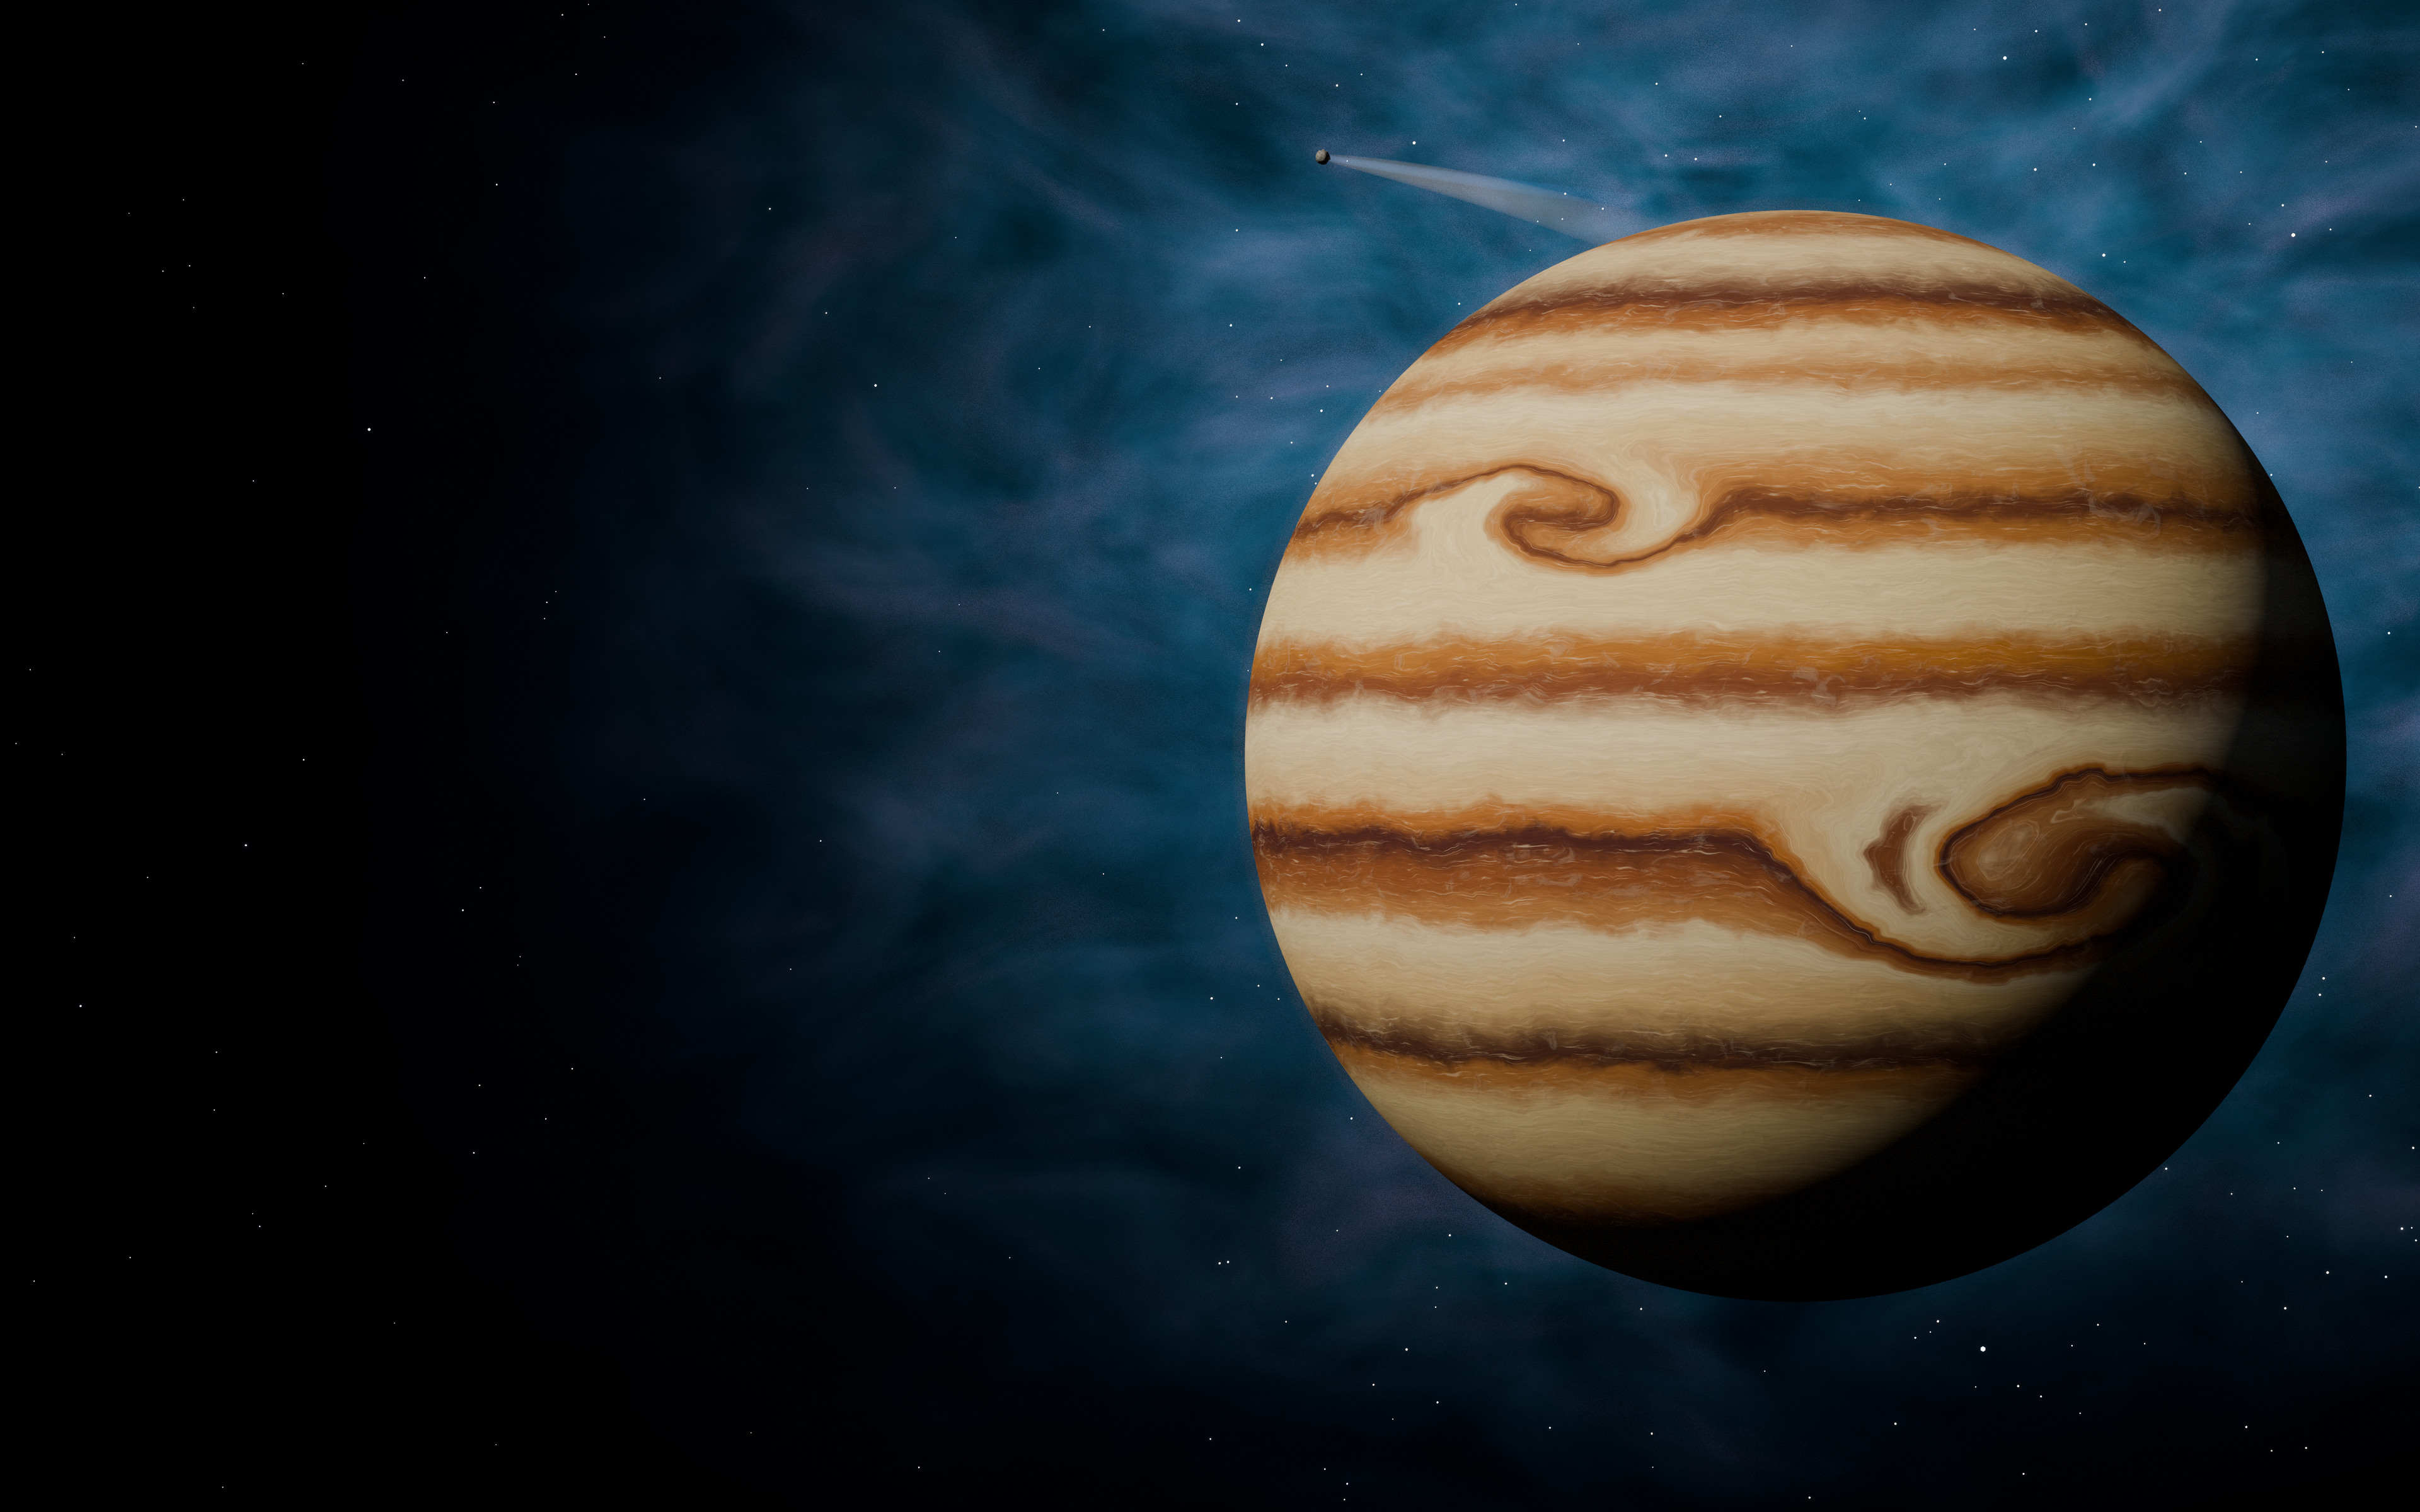
\includegraphics[width=\paperwidth,height=\paperheight]{Risorse/Copertine/M04_Aurea.jpg}};

\node[anchor=north west,inner sep=0,text width=9.2cm] at
 ([xshift=1.05cm,yshift=-1.10cm]current page.north west)
 {\color{Mint}\bfseries\fontsize{23}{27}\selectfont AUREA};
\node[anchor=north west,inner sep=0,text width=9.2cm] at
 ([xshift=1.07cm,yshift=-2.16cm]current page.north west)
 {\color{white}\fontsize{9.0}{12}\selectfont MODULO M04 · SCIENZE DELLA TERRA};
\draw[Mint,line width=1.4pt] ([xshift=1.05cm,yshift=-2.78cm]current page.north west)--
 ([xshift=2.60cm,yshift=-2.78cm]current page.north west);
\node[anchor=north west,inner sep=0] at
 ([xshift=1.05cm,yshift=-3.35cm]current page.north west)
 {\begin{minipage}{9.2cm}\raggedright\color{white}\bfseries
 \fontsize{30}{36}\selectfont Probabilità,\\variabilità e\\simulazione\end{minipage}};
\node[anchor=north west,inner sep=0] at
 ([xshift=1.07cm,yshift=-7.88cm]current page.north west)
 {\begin{minipage}{9.0cm}\raggedright\color{Lilac}
 \fontsize{12.2}{17}\selectfont Modelli probabilistici e propagazione\\dell’incertezza\end{minipage}};
\node[anchor=north west,inner sep=0,text width=9.2cm] at
 ([xshift=1.07cm,yshift=-10.52cm]current page.north west)
 {\color{white}\fontsize{11.5}{15}\selectfont Marzio De Corato};
\node[anchor=north west,inner sep=0,text width=9.2cm] at
 ([xshift=1.07cm,yshift=-11.17cm]current page.north west)
 {\color{Lilac}\fontsize{8.8}{11}\selectfont \href{https://creativecommons.org/licenses/by-nc-sa/4.0/}{\textcopyright{} 2026 · CC BY-NC-SA 4.0}};
\end{tikzpicture}
\end{frame}


\begin{frame}[plain]\hypertarget{slide2}{}
\bookmark[level=0,page=2]{Domanda centrale}
\begin{tikzpicture}[remember picture,overlay]
\node[anchor=north west,inner sep=0] at ([xshift=.95cm,yshift=-.67cm]current page.north west) {\color{Navy}\bfseries\fontsize{23}{27}\selectfont Come modellare la variabilità?};
\draw[Classical,line width=1.4pt] ([xshift=.95cm,yshift=-1.73cm]current page.north west)--([xshift=2.5cm,yshift=-1.73cm]current page.north west);
\node[anchor=north west,inner sep=0,fill=GeoTint,rounded corners=2mm,text width=17.7cm,inner sep=3.5mm] at ([xshift=1.0cm,yshift=-2.26cm]current page.north west) {\color{Navy}\fontsize{14.1}{19}\selectfont Quali ipotesi permettono di trasformare l’incertezza in probabilità?};
\node[draw=Rule,line width=.7pt,fill=GeoTint,rounded corners=2.5mm,minimum width=4.8cm,minimum height=2.15cm,text width=4.38cm,align=center,inner sep=3mm] (n0) at ([xshift=4cm,yshift=-6.15cm]current page.north west) {\color{Navy}\bfseries\fontsize{13}{16}\selectfont IPOTESI\\[2mm]\color{Ink}\normalfont\fontsize{10.5}{14}\selectfont Eventi e distribuzioni};
\node[draw=Rule,line width=.7pt,fill=Paper,rounded corners=2.5mm,minimum width=4.8cm,minimum height=2.15cm,text width=4.38cm,align=center,inner sep=3mm] (n1) at ([xshift=10cm,yshift=-6.15cm]current page.north west) {\color{Navy}\bfseries\fontsize{13}{16}\selectfont SIMULAZIONE\\[2mm]\color{Ink}\normalfont\fontsize{10.5}{14}\selectfont Repliche e Monte Carlo};
\node[draw=Rule,line width=.7pt,fill=GeoTint,rounded corners=2.5mm,minimum width=4.8cm,minimum height=2.15cm,text width=4.38cm,align=center,inner sep=3mm] (n2) at ([xshift=16cm,yshift=-6.15cm]current page.north west) {\color{Navy}\bfseries\fontsize{13}{16}\selectfont PROPAGAZIONE\\[2mm]\color{Ink}\normalfont\fontsize{10.5}{14}\selectfont Risultati e dipendenza};
\draw[-{Stealth[length=3.0mm]},draw=Classical,line width=1.45pt] ([xshift=6.65cm,yshift=-6.15cm]current page.north west)--([xshift=7.35cm,yshift=-6.15cm]current page.north west);
\draw[-{Stealth[length=3.0mm]},draw=Classical,line width=1.45pt] ([xshift=12.65cm,yshift=-6.15cm]current page.north west)--([xshift=13.35cm,yshift=-6.15cm]current page.north west);
\node[anchor=north west,inner sep=0,text width=17.9cm] at ([xshift=1.05cm,yshift=-8.25cm]current page.north west) {\color{Classical}\bfseries\fontsize{10.4}{13.4}\selectfont IDEA GUIDA};
\node[anchor=north west,inner sep=0,text width=17.85cm] at ([xshift=1.05cm,yshift=-8.71cm]current page.north west) {\color{Ink}\fontsize{11.9}{16.0}\selectfont La simulazione quantifica le conseguenze di un modello; non sostituisce la verifica delle sue ipotesi o della qualità degli ingressi.};
\draw[Rule,line width=.35pt] ([xshift=.95cm,yshift=-11.92cm]current page.north west)--([xshift=19.05cm,yshift=-11.92cm]current page.north west);
\node[anchor=north west,inner sep=0] at ([xshift=.95cm,yshift=-12.06cm]current page.north west) {\color{Muted}\fontsize{7.7}{9.3}\selectfont Aurea · Probabilità, variabilità e simulazione};
\node[anchor=north east,inner sep=0] at ([xshift=19.05cm,yshift=-12.06cm]current page.north west) {\color{Muted}\fontsize{7.7}{9.3}\selectfont 2/81};
\end{tikzpicture}
\end{frame}
% SLIDE 003 | Un modello per le ripetizioni possibili
\begin{lrbox}{\PilotLeftBox}%
\begin{minipage}[t]{10.05cm}\raggedright\color{Ink}\fontsize{11.3}{14.8}\selectfont

\PLabel{Dalla domanda alle conseguenze del modello}
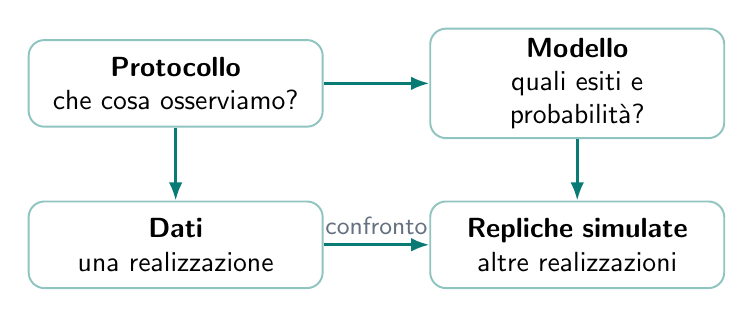
\begin{tikzpicture}[x=1cm,y=1cm]
\node[pFlow,text width=3.5cm] (p) at(2,3.3){\textbf{Protocollo}\\che cosa osserviamo?};
\node[pFlow,text width=3.5cm] (m) at(7.1,3.3){\textbf{Modello}\\quali esiti e probabilità?};
\node[pFlow,text width=3.5cm] (d) at(2,1.25){\textbf{Dati}\\una realizzazione};
\node[pFlow,text width=3.5cm] (r) at(7.1,1.25){\textbf{Repliche simulate}\\altre realizzazioni};
\draw[pEdge](p)--(m);\draw[pEdge](p)--(d);\draw[pEdge](m)--(r);
\draw[pEdge](d)--node[pNote,above]{confronto}(r);
\end{tikzpicture}
\PBody{Iride ha descritto le osservazioni. In Aurea assegniamo probabilità agli esiti e calcoliamo ciò che il modello prevede.}

\end{minipage}% 
\end{lrbox}
\typeout{FULLBOX:003:L:\the\ht\PilotLeftBox:\the\dp\PilotLeftBox}
\begin{lrbox}{\PilotRightBox}%
\begin{minipage}[t]{7.55cm}\raggedright\color{Ink}\fontsize{11.3}{14.8}\selectfont

\PCode{R · progetto della lezione}{03_avvio.R}
\PSmall{\texttt{setup.R} definisce le funzioni dei laboratori e legge i parametri di massa e volume. Non avvia simulazioni.}
\PInfo{Prerequisiti: vettori, selezioni logiche, media, deviazione standard e lettura dei grafici. Il codice completo è in \texttt{Lezione\_Aurea.R}.}

\end{minipage}% 
\end{lrbox}
\typeout{FULLBOX:003:R:\the\ht\PilotRightBox:\the\dp\PilotRightBox}
\begin{frame}[plain]\hypertarget{slide3}{}
\bookmark[level=1,page=3]{Un modello per le ripetizioni possibili}
\begin{tikzpicture}[remember picture,overlay]
\PilotChrome{Un modello per le ripetizioni possibili}{EVENTI E PROBABILITÀ}{3}{Un modello probabilistico rende espliciti gli esiti, le probabilità assegnate e le condizioni delle ripetizioni.}
\node[anchor=north west,inner sep=0] at ([xshift=0.96cm,yshift=-2.13cm]current page.north west) {\usebox{\PilotLeftBox}};
\node[anchor=north west,inner sep=0] at ([xshift=11.52cm,yshift=-2.13cm]current page.north west) {\usebox{\PilotRightBox}};

\end{tikzpicture}\end{frame}

% SLIDE 004 | Tre origini diverse della variabilità
\begin{lrbox}{\FullWideBox}%
\begin{minipage}[t]{18.1cm}\raggedright\color{Ink}\fontsize{11.3}{14.8}\selectfont

\PLabel{Che cosa varia e che cosa possiamo modificare}
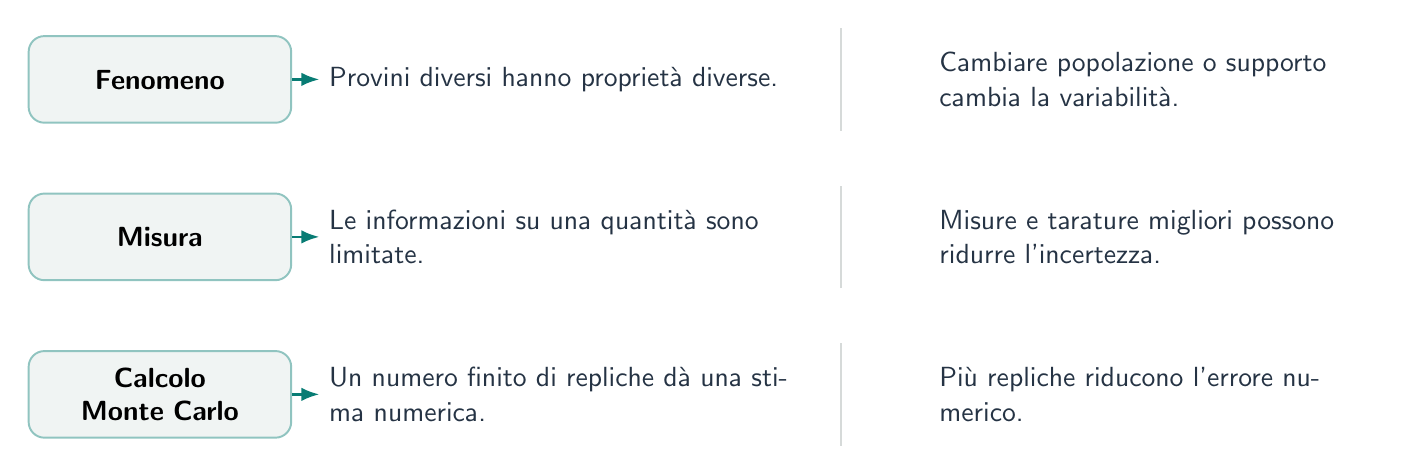
\begin{tikzpicture}[x=1cm,y=1cm]
\foreach \yy/\lab/\desc/\act in {
5/{Fenomeno}/{Provini diversi hanno proprietà diverse.}/{Cambiare popolazione o supporto cambia la variabilità.},
3/{Misura}/{Le informazioni su una quantità sono limitate.}/{Misure e tarature migliori possono ridurre l'incertezza.},
1/{Calcolo Monte Carlo}/{Un numero finito di repliche dà una stima numerica.}/{Più repliche riducono l'errore numerico.}}{
\node[pFlow,text width=3.1cm,fill=GeoTint] (a\yy) at(1.8,\yy){\textbf{\lab}};
\node[pLabel,text width=6.1cm,align=left] (b\yy) at(7,\yy){\desc};
\node[pLabel,text width=5.4cm,align=left] (c\yy) at(14.4,\yy){\act};
\draw[pEdge](a\yy)--(b\yy);
\draw[Rule](10.45,\yy-.65)--(10.45,\yy+.65);
}
\end{tikzpicture}
\PSmall{Il numero di repliche del computer non migliora da solo una misura, la rappresentatività dei dati o la scelta del modello.}

\end{minipage}% 
\end{lrbox}
\typeout{FULLBOX:004:W:\the\ht\FullWideBox:\the\dp\FullWideBox}
\begin{frame}[plain]\hypertarget{slide4}{}
\bookmark[level=1,page=4]{Tre origini diverse della variabilità}
\begin{tikzpicture}[remember picture,overlay]
\PilotChrome{Tre origini diverse della variabilità}{EVENTI E PROBABILITÀ}{4}{Prima di parlare di precisione, occorre identificare la quantità che varia e la fonte di quella variazione.}
\node[anchor=north west,inner sep=0] at ([xshift=0.96cm,yshift=-2.13cm]current page.north west) {\usebox{\FullWideBox}};

\end{tikzpicture}\end{frame}

% SLIDE 005 | Esiti ed eventi in un insieme finito
\begin{lrbox}{\PilotLeftBox}%
\begin{minipage}[t]{10.05cm}\raggedright\color{Ink}\fontsize{11.3}{14.8}\selectfont

\PLabel{Un provino scelto con probabilità uniforme}
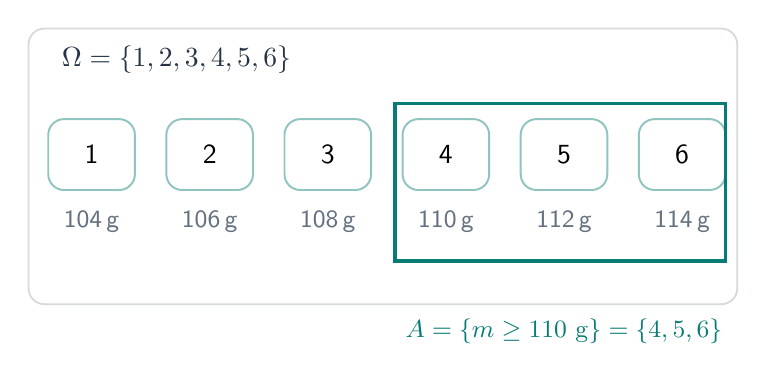
\begin{tikzpicture}[x=1cm,y=1cm]
\draw[pGroup](.2,0) rectangle(9.2,3.5);
\node[pLabel,anchor=west] at(.5,3.1){$\Omega=\{1,2,3,4,5,6\}$};
\foreach \x/\lab/\mass in {1/1/104,2.5/2/106,4/3/108,5.5/4/110,7/5/112,8.5/6/114}{
\node[pFlow,minimum width=1.1cm,minimum height=.9cm] at(\x,1.9){\lab};
\node[pNote] at(\x,1.05){\mass\,g};}
\draw[Classical,line width=1.3pt](4.85,.55) rectangle(9.05,2.55);
\node[pNote,text=Classical] at(7,-.35){$A=\{m\ge110\ \mathrm{g}\}=\{4,5,6\}$};
\end{tikzpicture}
\PBody{Un esito è il provino estratto. Un evento è un insieme di esiti che soddisfano una regola. Ogni provino ha probabilità $1/6$.}
\PSmall{La scelta uniforme è un'ipotesi esplicita di questo esempio costruito.}

\end{minipage}% 
\end{lrbox}
\typeout{FULLBOX:005:L:\the\ht\PilotLeftBox:\the\dp\PilotLeftBox}
\begin{lrbox}{\PilotRightBox}%
\begin{minipage}[t]{7.55cm}\raggedright\color{Ink}\fontsize{11.3}{14.8}\selectfont

\PCode{R · un evento come condizione}{05_eventi.R}
\PSmall{\texttt{A05} contiene valori \texttt{TRUE}/\texttt{FALSE}. La media conta i veri e divide per sei. Qui coincide con la probabilità perché tutti gli esiti sono equiprobabili.}
\PInfo{$0\le P(A)\le1,\quad P(\Omega)=1.$\\Il modello deve assegnare probabilità anche quando gli esiti hanno pesi diversi.}

\end{minipage}% 
\end{lrbox}
\typeout{FULLBOX:005:R:\the\ht\PilotRightBox:\the\dp\PilotRightBox}
\begin{frame}[plain]\hypertarget{slide5}{}
\bookmark[level=1,page=5]{Esiti ed eventi in un insieme finito}
\begin{tikzpicture}[remember picture,overlay]
\PilotChrome{Esiti ed eventi in un insieme finito}{EVENTI E PROBABILITÀ}{5}{La probabilità per conteggio richiede esiti equiprobabili e un evento definito senza ambiguità.}
\node[anchor=north west,inner sep=0] at ([xshift=0.96cm,yshift=-2.13cm]current page.north west) {\usebox{\PilotLeftBox}};
\node[anchor=north west,inner sep=0] at ([xshift=11.52cm,yshift=-2.13cm]current page.north west) {\usebox{\PilotRightBox}};

\end{tikzpicture}\end{frame}

% SLIDE 006 | Unione, intersezione e complemento
\begin{lrbox}{\PilotLeftBox}%
\begin{minipage}[t]{10.05cm}\raggedright\color{Ink}\fontsize{11.3}{14.8}\selectfont

\PLabel{Le operazioni sugli eventi}
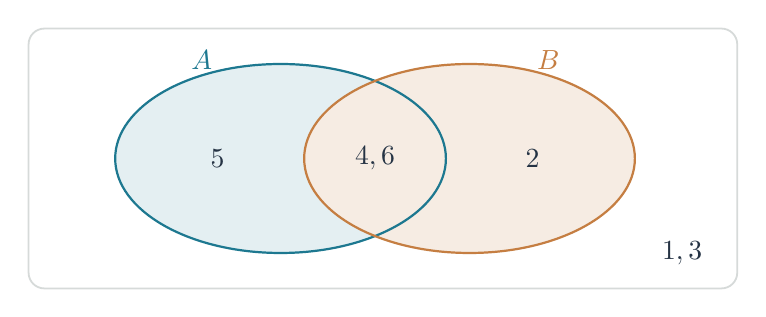
\begin{tikzpicture}[x=1cm,y=1cm]
\draw[pGroup](.2,.1) rectangle(9.2,3.4);
\fill[GeoA!12](3.4,1.75) ellipse(2.1cm and 1.2cm);
\fill[GeoB!15](5.8,1.75) ellipse(2.1cm and 1.2cm);
\draw[GeoA,line width=.8pt](3.4,1.75) ellipse(2.1cm and 1.2cm);
\draw[GeoB,line width=.8pt](5.8,1.75) ellipse(2.1cm and 1.2cm);
\node[pLabel] at(2.6,1.75){$5$};
\node[pLabel] at(4.6,1.75){$4,6$};
\node[pLabel] at(6.6,1.75){$2$};
\node[pLabel] at(8.5,.55){$1,3$};
\node[pLabel,text=GeoA] at(2.4,3){$A$};
\node[pLabel,text=GeoB] at(6.8,3){$B$};
\end{tikzpicture}
\[
P(A\cup B)=P(A)+P(B)-P(A\cap B)
\]
\PSmall{L'intersezione compare in entrambi i conteggi e va sottratta una volta. Il disegno rappresenta appartenenze, senza proporzionalità fra aree e probabilità.}

\end{minipage}% 
\end{lrbox}
\typeout{FULLBOX:006:L:\the\ht\PilotLeftBox:\the\dp\PilotLeftBox}
\begin{lrbox}{\PilotRightBox}%
\begin{minipage}[t]{7.55cm}\raggedright\color{Ink}\fontsize{11.3}{14.8}\selectfont

\PCode{R · operatori logici}{06_operazioni.R}
\PBody{\texttt{\&} richiede entrambe le condizioni. \texttt{|} richiede almeno una delle due. \texttt{!} inverte la condizione.}
\PInfo{Per il complemento:\\$P(A^c)=1-P(A)$.\\In questo esempio $P(A^c)=3/6$.}

\end{minipage}% 
\end{lrbox}
\typeout{FULLBOX:006:R:\the\ht\PilotRightBox:\the\dp\PilotRightBox}
\begin{frame}[plain]\hypertarget{slide6}{}
\bookmark[level=1,page=6]{Unione, intersezione e complemento}
\begin{tikzpicture}[remember picture,overlay]
\PilotChrome{Unione, intersezione e complemento}{EVENTI E PROBABILITÀ}{6}{Per l’unione si sottrae l’intersezione; per il complemento si sottrae la probabilità a uno.}
\node[anchor=north west,inner sep=0] at ([xshift=0.96cm,yshift=-2.13cm]current page.north west) {\usebox{\PilotLeftBox}};
\node[anchor=north west,inner sep=0] at ([xshift=11.52cm,yshift=-2.13cm]current page.north west) {\usebox{\PilotRightBox}};

\end{tikzpicture}\end{frame}

% SLIDE 007 | Probabilità e frequenza osservata
\begin{lrbox}{\PilotLeftBox}%
\begin{minipage}[t]{10.05cm}\raggedright\color{Ink}\fontsize{11.3}{14.8}\selectfont

\PLabel{Prove indipendenti con probabilità costante $p=0{,}3$}
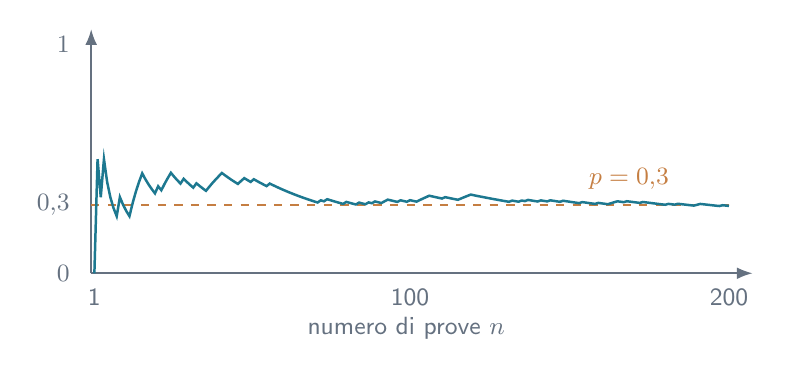
\begin{tikzpicture}[x=1cm,y=1cm]
\draw[pAxis](.5,.2)--(8.9,.2);\draw[pAxis](.5,.2)--(.5,3.3);
\foreach \y/\lab in {.2/0,1.07/{0{,}3},3.1/1}{\node[pNote,anchor=east] at(.35,\y){$\lab$};}
\foreach \x/\lab in {.54/1,4.55/100,8.6/200}{\node[pNote] at(\x,-.1){\lab};}
\draw[GeoB,dashed,line width=.8pt](.5,1.07)--(8.6,1.07);
\draw[GeoA,line width=.9pt] plot coordinates{(0.54050,0.20000) (0.58100,1.65000) (0.62150,1.16667) (0.66200,1.65000) (0.70250,1.36000) (0.74300,1.16667) (0.78350,1.02857) (0.82400,0.92500) (0.86450,1.16667) (0.90500,1.07000) (0.94550,0.99091) (0.98600,0.92500) (1.02650,1.09231) (1.06700,1.23571) (1.10750,1.36000) (1.14800,1.46875) (1.18850,1.39412) (1.22900,1.32778) (1.26950,1.26842) (1.31000,1.21500) (1.35050,1.30476) (1.39100,1.25455) (1.43150,1.33478) (1.47200,1.40833) (1.51250,1.47600) (1.55300,1.42692) (1.59350,1.38148) (1.63400,1.33929) (1.67450,1.40000) (1.71500,1.36000) (1.75550,1.32258) (1.79600,1.28750) (1.83650,1.34242) (1.87700,1.30882) (1.91750,1.27714) (1.95800,1.24722) (1.99850,1.29730) (2.03900,1.34474) (2.07950,1.38974) (2.12000,1.43250) (2.16050,1.47317) (2.20100,1.44286) (2.24150,1.41395) (2.28200,1.38636) (2.32250,1.36000) (2.36300,1.33478) (2.40350,1.37234) (2.44400,1.40833) (2.48450,1.38367) (2.52500,1.36000) (2.56550,1.39412) (2.60600,1.37115) (2.64650,1.34906) (2.68700,1.32778) (2.72750,1.30727) (2.76800,1.33929) (2.80850,1.31930) (2.84900,1.30000) (2.88950,1.28136) (2.93000,1.26333) (2.97050,1.24590) (3.01100,1.22903) (3.05150,1.21270) (3.09200,1.19687) (3.13250,1.18154) (3.17300,1.16667) (3.21350,1.15224) (3.25400,1.13824) (3.29450,1.12464) (3.33500,1.11143) (3.37550,1.09859) (3.41600,1.12639) (3.45650,1.11370) (3.49700,1.14054) (3.53750,1.12800) (3.57800,1.11579) (3.61850,1.10390) (3.65900,1.09231) (3.69950,1.08101) (3.74000,1.10625) (3.78050,1.09506) (3.82100,1.08415) (3.86150,1.07349) (3.90200,1.09762) (3.94250,1.08706) (3.98300,1.07674) (4.02350,1.10000) (4.06400,1.08977) (4.10450,1.11236) (4.14500,1.10222) (4.18550,1.09231) (4.22600,1.11413) (4.26650,1.13548) (4.30700,1.12553) (4.34750,1.11579) (4.38800,1.10625) (4.42850,1.12680) (4.46900,1.11735) (4.50950,1.10808) (4.55000,1.12800) (4.59050,1.11881) (4.63100,1.10980) (4.67150,1.12913) (4.71200,1.14808) (4.75250,1.16667) (4.79300,1.18491) (4.83350,1.17570) (4.87400,1.16667) (4.91450,1.15780) (4.95500,1.14909) (4.99550,1.16667) (5.03600,1.15804) (5.07650,1.14956) (5.11700,1.14123) (5.15750,1.13304) (5.19800,1.15000) (5.23850,1.16667) (5.27900,1.18305) (5.31950,1.19916) (5.36000,1.19083) (5.40050,1.18264) (5.44100,1.17459) (5.48150,1.16667) (5.52200,1.15887) (5.56250,1.15120) (5.60300,1.14365) (5.64350,1.13622) (5.68400,1.12891) (5.72450,1.12171) (5.76500,1.11462) (5.80550,1.10763) (5.84600,1.12273) (5.88650,1.11579) (5.92700,1.10896) (5.96750,1.12370) (6.00800,1.11691) (6.04850,1.13139) (6.08900,1.12464) (6.12950,1.11799) (6.17000,1.11143) (6.21050,1.12553) (6.25100,1.11901) (6.29150,1.11259) (6.33200,1.12639) (6.37250,1.12000) (6.41300,1.11370) (6.45350,1.10748) (6.49400,1.12095) (6.53450,1.11477) (6.57500,1.10867) (6.61550,1.10265) (6.65600,1.09671) (6.69650,1.09085) (6.73700,1.10390) (6.77750,1.09806) (6.81800,1.09231) (6.85850,1.08662) (6.89900,1.08101) (6.93950,1.09371) (6.98000,1.08813) (7.02050,1.08261) (7.06100,1.07716) (7.10150,1.08957) (7.14200,1.10183) (7.18250,1.11394) (7.22300,1.10843) (7.26350,1.10299) (7.30400,1.11488) (7.34450,1.10947) (7.38500,1.10412) (7.42550,1.09883) (7.46600,1.09360) (7.50650,1.10520) (7.54700,1.10000) (7.58750,1.09486) (7.62800,1.08977) (7.66850,1.08475) (7.70900,1.07978) (7.74950,1.07486) (7.79000,1.07000) (7.83050,1.08122) (7.87100,1.07637) (7.91150,1.07158) (7.95200,1.08261) (7.99250,1.07784) (8.03300,1.07312) (8.07350,1.06845) (8.11400,1.06383) (8.15450,1.05926) (8.19500,1.07000) (8.23550,1.08063) (8.27600,1.07604) (8.31650,1.07150) (8.35700,1.06701) (8.39750,1.06256) (8.43800,1.05816) (8.47850,1.05381) (8.51900,1.06414) (8.55950,1.05980) (8.60000,1.05550)};
\node[pNote,anchor=west,text=GeoB] at(6.7,1.4){$p=0{,}3$};
\node[pNote] at(4.5,-.5){numero di prove $n$};
\end{tikzpicture}
\[
\widehat p_n=\frac1n\sum_{i=1}^{n} I_i,\qquad I_i=\mathbf1_{\{A\text{ alla prova }i\}}.
\]
\PSmall{Le oscillazioni possono aumentare temporaneamente lo scarto da $p$.}

\end{minipage}% 
\end{lrbox}
\typeout{FULLBOX:007:L:\the\ht\PilotLeftBox:\the\dp\PilotLeftBox}
\begin{lrbox}{\PilotRightBox}%
\begin{minipage}[t]{7.55cm}\raggedright\color{Ink}\fontsize{11.3}{14.8}\selectfont

\PCode{R · frequenza cumulativa}{07_frequenza.R}
\PSmall{\texttt{rbinom(200,1,.3)} genera 200 esiti 0/1. \texttt{cumsum()} conta progressivamente gli eventi. Il denominatore cresce a ogni prova.}
\PInfo{$p$ resta fisso. La frequenza cambia con la sequenza e il numero di prove.}

\end{minipage}% 
\end{lrbox}
\typeout{FULLBOX:007:R:\the\ht\PilotRightBox:\the\dp\PilotRightBox}
\begin{frame}[plain]\hypertarget{slide7}{}
\bookmark[level=1,page=7]{Probabilità e frequenza osservata}
\begin{tikzpicture}[remember picture,overlay]
\PilotChrome{Probabilità e frequenza osservata}{EVENTI E PROBABILITÀ}{7}{La probabilità è un parametro del modello; la frequenza è una quantità calcolata da una realizzazione.}
\node[anchor=north west,inner sep=0] at ([xshift=0.96cm,yshift=-2.13cm]current page.north west) {\usebox{\PilotLeftBox}};
\node[anchor=north west,inner sep=0] at ([xshift=11.52cm,yshift=-2.13cm]current page.north west) {\usebox{\PilotRightBox}};

\end{tikzpicture}\end{frame}

% SLIDE 008 | Il valore atteso di un conteggio
\begin{lrbox}{\PilotLeftBox}%
\begin{minipage}[t]{10.05cm}\raggedright\color{Ink}\fontsize{11.3}{14.8}\selectfont

\PLabel{Un modello con tre esiti numerici}
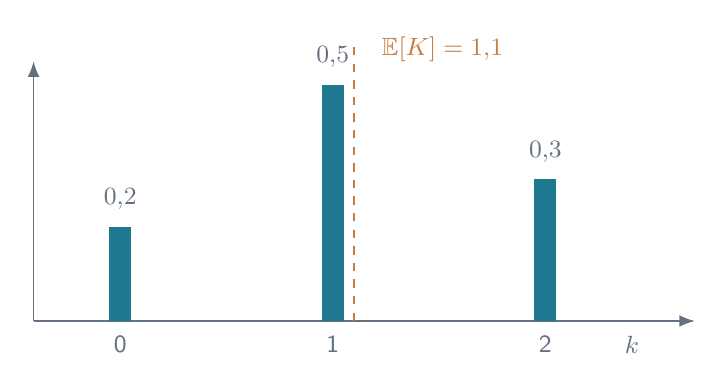
\begin{tikzpicture}[x=1cm,y=1cm]
\draw[pAxis](.4,.2)--(8.8,.2);\draw[pAxis](.4,.2)--(.4,3.5);
\foreach \x/\y/\lab in {1.5/1.4/{0{,}2},4.2/3.2/{0{,}5},6.9/2/{0{,}3}}{
\draw[GeoA,line width=8pt](\x,.2)--(\x,\y);\node[pNote] at(\x,\y+.35){$\lab$};}
\foreach \x/\lab in {1.5/0,4.2/1,6.9/2}{\node[pNote] at(\x,-.1){\lab};}
\draw[GeoB,dashed,line width=.9pt](4.47,.2)--(4.47,3.7);
\node[pNote,text=GeoB,anchor=west] at(4.7,3.65){$\mathbb E[K]=1{,}1$};
\node[pNote] at(8,-.1){$k$};
\end{tikzpicture}
\[
\mathbb E[K]=\sum_k kP(K=k)
=0\cdot0{,}2+1\cdot0{,}5+2\cdot0{,}3=1{,}1.
\]
\PSmall{L'atteso può essere diverso da tutti i valori ammessi per una singola osservazione.}

\end{minipage}% 
\end{lrbox}
\typeout{FULLBOX:008:L:\the\ht\PilotLeftBox:\the\dp\PilotLeftBox}
\begin{lrbox}{\PilotRightBox}%
\begin{minipage}[t]{7.55cm}\raggedright\color{Ink}\fontsize{11.3}{14.8}\selectfont

\PCode{R · media del modello}{08_atteso.R}
\PSmall{\texttt{sample()} estrae i valori $0,1,2$ con i pesi specificati. \texttt{replace=TRUE} permette estrazioni ripetute dallo stesso insieme.}
\PInfo{L'atteso descrive il centro delle ripetizioni. Il conteggio effettivo rimane un intero.}

\end{minipage}% 
\end{lrbox}
\typeout{FULLBOX:008:R:\the\ht\PilotRightBox:\the\dp\PilotRightBox}
\begin{frame}[plain]\hypertarget{slide8}{}
\bookmark[level=1,page=8]{Il valore atteso di un conteggio}
\begin{tikzpicture}[remember picture,overlay]
\PilotChrome{Il valore atteso di un conteggio}{EVENTI E PROBABILITÀ}{8}{Il valore atteso è una media pesata delle possibilità del modello; la singola prova conserva i propri esiti ammessi.}
\node[anchor=north west,inner sep=0] at ([xshift=0.96cm,yshift=-2.13cm]current page.north west) {\usebox{\PilotLeftBox}};
\node[anchor=north west,inner sep=0] at ([xshift=11.52cm,yshift=-2.13cm]current page.north west) {\usebox{\PilotRightBox}};

\end{tikzpicture}\end{frame}

% SLIDE 009 | Laboratorio: frequenze nelle ripetizioni
\begin{lrbox}{\PilotLeftBox}%
\begin{minipage}[t]{10.05cm}\raggedright\color{Ink}\fontsize{11.3}{14.8}\selectfont

\PLab{https://marzione00.github.io/Lab_Geo/\#laboratorio/m04-eventi}{Esperimento m04-eventi}
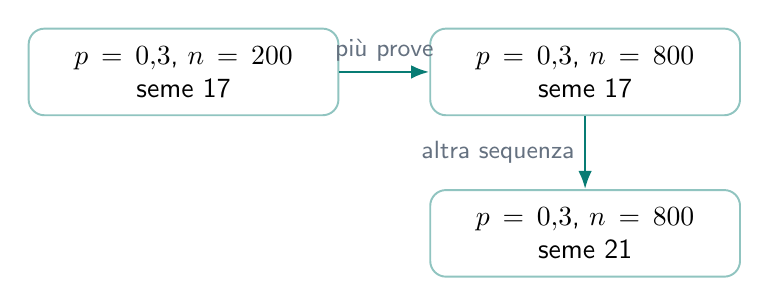
\begin{tikzpicture}[x=1cm,y=1cm]
\node[pFlow,text width=3.7cm] (a) at(2.1,3.3){$p=0{,}3$, $n=200$\\seme 17};
\node[pFlow,text width=3.7cm] (b) at(7.2,3.3){$p=0{,}3$, $n=800$\\seme 17};
\node[pFlow,text width=3.7cm] (c) at(7.2,1.25){$p=0{,}3$, $n=800$\\seme 21};
\draw[pEdge](a)--node[pNote,above]{più prove}(b);
\draw[pEdge](b)--node[pNote,left]{altra sequenza}(c);
\end{tikzpicture}
\PBody{Registrare la frequenza finale e il suo scarto da $p$. Cercare anche un tratto in cui lo scarto aumenta.}
\PSmall{Il sito consente da 20 a 2000 prove. L'esperimento mantiene indipendenza e probabilità costante.}

\end{minipage}% 
\end{lrbox}
\typeout{FULLBOX:009:L:\the\ht\PilotLeftBox:\the\dp\PilotLeftBox}
\begin{lrbox}{\PilotRightBox}%
\begin{minipage}[t]{7.55cm}\raggedright\color{Ink}\fontsize{11.3}{14.8}\selectfont

\PCode{R · confronti controllati}{09_lab_eventi.R}
\PSmall{Le funzioni del progetto riproducono i dati e gli indicatori degli esperimenti. \texttt{\$indicatori} estrae il riepilogo restituito dalla funzione.}
\PInfo{Domanda: una frequenza finale più vicina a $p$ dimostra che la convergenza è sempre monotona? Motivare dalla curva.}

\end{minipage}% 
\end{lrbox}
\typeout{FULLBOX:009:R:\the\ht\PilotRightBox:\the\dp\PilotRightBox}
\begin{frame}[plain]\hypertarget{slide9}{}
\bookmark[level=1,page=9]{Laboratorio: frequenze nelle ripetizioni}
\begin{tikzpicture}[remember picture,overlay]
\PilotChrome{Laboratorio: frequenze nelle ripetizioni}{LABORATORIO · EVENTI}{9}{Il numero di prove e il seme modificano la realizzazione; il parametro p definisce la probabilità dell’evento.}
\node[anchor=north west,inner sep=0] at ([xshift=0.96cm,yshift=-2.13cm]current page.north west) {\usebox{\PilotLeftBox}};
\node[anchor=north west,inner sep=0] at ([xshift=11.52cm,yshift=-2.13cm]current page.north west) {\usebox{\PilotRightBox}};

\end{tikzpicture}\end{frame}

% SLIDE 010 | Condizionare cambia il denominatore
\begin{lrbox}{\PilotLeftBox}%
\begin{minipage}[t]{10.05cm}\raggedright\color{Ink}\fontsize{11.3}{14.8}\selectfont

\PLabel{Modello di un segnale A e di un tipo B}
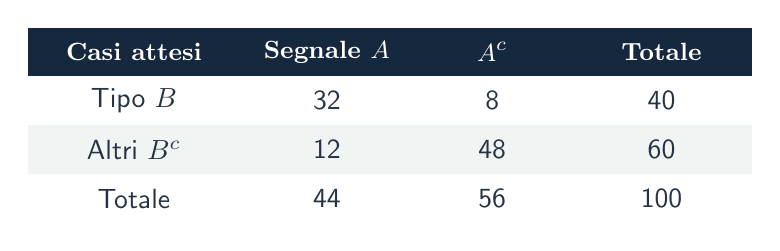
\begin{tikzpicture}[x=1cm,y=1cm]
\fill[Navy](0,0) rectangle(9.2,0.62);
\node[font=\bfseries\fontsize{9.5}{12}\selectfont,text=white] at(1.35,0.31){Casi attesi};
\node[font=\bfseries\fontsize{9.5}{12}\selectfont,text=white] at(3.8000000000000003,0.31){Segnale $A$};
\node[font=\bfseries\fontsize{9.5}{12}\selectfont,text=white] at(5.9,0.31){$A^c$};
\node[font=\bfseries\fontsize{9.5}{12}\selectfont,text=white] at(8.05,0.31){Totale};
\fill[white](0,-0.62) rectangle(9.2,0.0);
\node[pLabel] at(1.35,-0.31){Tipo $B$};
\node[pLabel] at(3.8000000000000003,-0.31){32};
\node[pLabel] at(5.9,-0.31){8};
\node[pLabel] at(8.05,-0.31){40};
\fill[GeoTint](0,-1.24) rectangle(9.2,-0.62);
\node[pLabel] at(1.35,-0.9299999999999999){Altri $B^c$};
\node[pLabel] at(3.8000000000000003,-0.9299999999999999){12};
\node[pLabel] at(5.9,-0.9299999999999999){48};
\node[pLabel] at(8.05,-0.9299999999999999){60};
\fill[white](0,-1.8599999999999999) rectangle(9.2,-1.2399999999999998);
\node[pLabel] at(1.35,-1.5499999999999998){Totale};
\node[pLabel] at(3.8000000000000003,-1.5499999999999998){44};
\node[pLabel] at(5.9,-1.5499999999999998){56};
\node[pLabel] at(8.05,-1.5499999999999998){100};
\end{tikzpicture}
\vspace{2mm}
\[
P(A\mid B)=\frac{P(A\cap B)}{P(B)}=\frac{32}{40}=0{,}8.
\]
\PSmall{I conteggi sono attesi, costruiti da probabilità assegnate. La popolazione di riferimento comprende entrambi i tipi.}
\PBody{Conoscere $B$ restringe l'insieme di riferimento alla prima riga.}

\end{minipage}% 
\end{lrbox}
\typeout{FULLBOX:010:L:\the\ht\PilotLeftBox:\the\dp\PilotLeftBox}
\begin{lrbox}{\PilotRightBox}%
\begin{minipage}[t]{7.55cm}\raggedright\color{Ink}\fontsize{11.3}{14.8}\selectfont

\PCode{R · selezionare il denominatore}{10_condizionata.R}
\PSmall{Le righe distinguono i tipi, le colonne il segnale. \texttt{sum(t10["B",])} conta tutti i casi del gruppo $B$.}
\PInfo{La definizione richiede $P(B)>0$. Una condizione impossibile non fornisce un denominatore utilizzabile.}

\end{minipage}% 
\end{lrbox}
\typeout{FULLBOX:010:R:\the\ht\PilotRightBox:\the\dp\PilotRightBox}
\begin{frame}[plain]\hypertarget{slide10}{}
\bookmark[level=1,page=10]{Condizionare cambia il denominatore}
\begin{tikzpicture}[remember picture,overlay]
\PilotChrome{Condizionare cambia il denominatore}{CONDIZIONAMENTO}{10}{Una probabilità condizionata deve sempre dichiarare il gruppo entro cui si calcola la quota.}
\node[anchor=north west,inner sep=0] at ([xshift=0.96cm,yshift=-2.13cm]current page.north west) {\usebox{\PilotLeftBox}};
\node[anchor=north west,inner sep=0] at ([xshift=11.52cm,yshift=-2.13cm]current page.north west) {\usebox{\PilotRightBox}};

\end{tikzpicture}\end{frame}

% SLIDE 011 | Probabilità congiunte e probabilità totale
\begin{lrbox}{\PilotLeftBox}%
\begin{minipage}[t]{10.05cm}\raggedright\color{Ink}\fontsize{11.3}{14.8}\selectfont

\PLabel{Prodotti lungo i percorsi, somme fra percorsi alternativi}
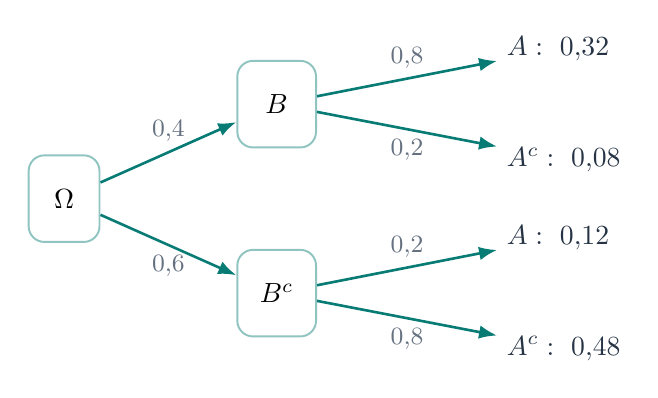
\begin{tikzpicture}[x=1cm,y=1cm]
\node[pFlow,minimum width=.9cm] (o) at(.7,2.1){$\Omega$};
\node[pFlow,minimum width=1cm] (b) at(3.4,3.3){$B$};
\node[pFlow,minimum width=1cm] (c) at(3.4,.9){$B^c$};
\node[pLabel,anchor=west] (a) at(6.2,4){$A:\ 0{,}32$};
\node[pLabel,anchor=west] (aa) at(6.2,2.6){$A^c:\ 0{,}08$};
\node[pLabel,anchor=west] (ac) at(6.2,1.6){$A:\ 0{,}12$};
\node[pLabel,anchor=west] (cc) at(6.2,.2){$A^c:\ 0{,}48$};
\draw[pEdge](o)--node[pNote,above]{$0{,}4$}(b);
\draw[pEdge](o)--node[pNote,below]{$0{,}6$}(c);
\draw[pEdge](b)--node[pNote,above]{$0{,}8$}(a);
\draw[pEdge](b)--node[pNote,below]{$0{,}2$}(aa);
\draw[pEdge](c)--node[pNote,above]{$0{,}2$}(ac);
\draw[pEdge](c)--node[pNote,below]{$0{,}8$}(cc);
\end{tikzpicture}
\[
P(A)=P(A\mid B)P(B)+P(A\mid B^c)P(B^c).
\]
\PSmall{$B$ e $B^c$ sono disgiunti e ricoprono tutti gli esiti.}

\end{minipage}% 
\end{lrbox}
\typeout{FULLBOX:011:L:\the\ht\PilotLeftBox:\the\dp\PilotLeftBox}
\begin{lrbox}{\PilotRightBox}%
\begin{minipage}[t]{7.55cm}\raggedright\color{Ink}\fontsize{11.3}{14.8}\selectfont

\PCode{R · sommare i contributi}{11_totale.R}
\PBody{Il primo contributo è $0{,}8\cdot0{,}4=0{,}32$. Il secondo è $0{,}2\cdot0{,}6=0{,}12$. La somma dà $P(A)=0{,}44$.}
\PInfo{La formula del prodotto $P(A\cap B)=P(A\mid B)P(B)$ vale anche quando gli eventi dipendono l'uno dall'altro.}

\end{minipage}% 
\end{lrbox}
\typeout{FULLBOX:011:R:\the\ht\PilotRightBox:\the\dp\PilotRightBox}
\begin{frame}[plain]\hypertarget{slide11}{}
\bookmark[level=1,page=11]{Probabilità congiunte e probabilità totale}
\begin{tikzpicture}[remember picture,overlay]
\PilotChrome{Probabilità congiunte e probabilità totale}{CONDIZIONAMENTO}{11}{La probabilità totale combina le probabilità interne ai gruppi usando i pesi dei gruppi.}
\node[anchor=north west,inner sep=0] at ([xshift=0.96cm,yshift=-2.13cm]current page.north west) {\usebox{\PilotLeftBox}};
\node[anchor=north west,inner sep=0] at ([xshift=11.52cm,yshift=-2.13cm]current page.north west) {\usebox{\PilotRightBox}};

\end{tikzpicture}\end{frame}

% SLIDE 012 | Indipendenza e incompatibilità
\begin{lrbox}{\PilotLeftBox}%
\begin{minipage}[t]{10.05cm}\raggedright\color{Ink}\fontsize{11.3}{14.8}\selectfont

\PLabel{Due relazioni con condizioni diverse}
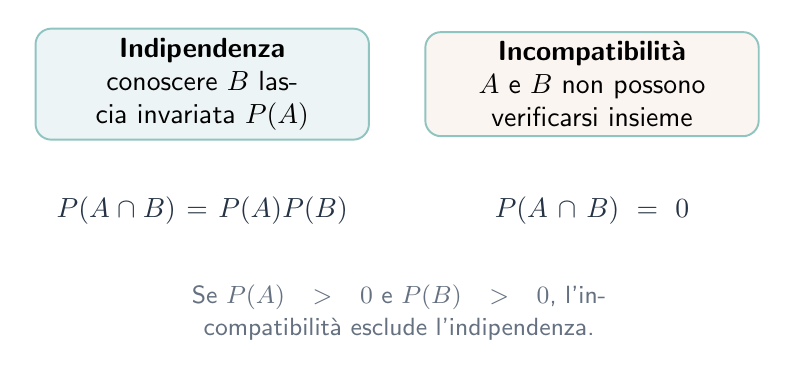
\begin{tikzpicture}[x=1cm,y=1cm]
\node[pFlow,text width=4cm,fill=GeoA!8] at(2.2,3.2){\textbf{Indipendenza}\\conoscere $B$ lascia invariata $P(A)$};
\node[pFlow,text width=4cm,fill=GeoB!8] at(7.15,3.2){\textbf{Incompatibilità}\\$A$ e $B$ non possono verificarsi insieme};
\node[pLabel,text width=4.2cm] at(2.2,1.6){$P(A\cap B)=P(A)P(B)$};
\node[pLabel,text width=4.2cm] at(7.15,1.6){$P(A\cap B)=0$};
\node[pNote,text width=9cm] at(4.7,.3){Se $P(A)>0$ e $P(B)>0$, l'incompatibilità esclude l'indipendenza.};
\end{tikzpicture}
\PBody{L'indipendenza è una proprietà del modello. Distanza fisica o assenza di una correlazione osservata non bastano a giustificarla.}

\end{minipage}% 
\end{lrbox}
\typeout{FULLBOX:012:L:\the\ht\PilotLeftBox:\the\dp\PilotLeftBox}
\begin{lrbox}{\PilotRightBox}%
\begin{minipage}[t]{7.55cm}\raggedright\color{Ink}\fontsize{11.3}{14.8}\selectfont

\PCode{R · una verifica numerica}{12_indipendenza.R}
\PSmall{\texttt{all.equal()} confronta valori numerici con tolleranza. \texttt{isTRUE()} converte l'esito della verifica in un singolo valore logico.}
\PInfo{Nel modello della pagina precedente, $P(A\mid B)=0{,}8$ e $P(A)=0{,}44$: gli eventi sono dipendenti.}

\end{minipage}% 
\end{lrbox}
\typeout{FULLBOX:012:R:\the\ht\PilotRightBox:\the\dp\PilotRightBox}
\begin{frame}[plain]\hypertarget{slide12}{}
\bookmark[level=1,page=12]{Indipendenza e incompatibilità}
\begin{tikzpicture}[remember picture,overlay]
\PilotChrome{Indipendenza e incompatibilità}{CONDIZIONAMENTO}{12}{L’indipendenza conserva la probabilità dopo il condizionamento; l’incompatibilità vieta il verificarsi congiunto.}
\node[anchor=north west,inner sep=0] at ([xshift=0.96cm,yshift=-2.13cm]current page.north west) {\usebox{\PilotLeftBox}};
\node[anchor=north west,inner sep=0] at ([xshift=11.52cm,yshift=-2.13cm]current page.north west) {\usebox{\PilotRightBox}};

\end{tikzpicture}\end{frame}

% SLIDE 013 | La probabilità inversa con Bayes
\begin{lrbox}{\PilotLeftBox}%
\begin{minipage}[t]{10.05cm}\raggedright\color{Ink}\fontsize{11.3}{14.8}\selectfont

\PLabel{Fra i casi con segnale A}
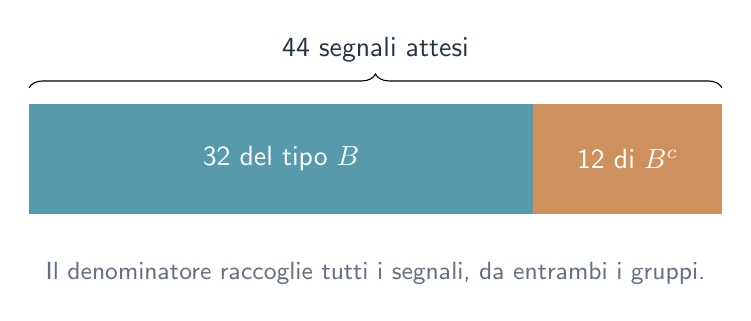
\begin{tikzpicture}[x=1cm,y=1cm]
\fill[GeoA!75](.4,1.3) rectangle(6.8,2.7);
\fill[GeoB!85](6.8,1.3) rectangle(9.2,2.7);
\node[pLabel,text=white] at(3.6,2){32 del tipo $B$};
\node[pLabel,text=white] at(8,2){12 di $B^c$};
\draw[decorate,decoration={brace,amplitude=5pt}](.4,2.9)--(9.2,2.9)
 node[midway,above=6pt,pLabel]{44 segnali attesi};
\node[pNote,text width=8.6cm] at(4.8,.55){Il denominatore raccoglie tutti i segnali, da entrambi i gruppi.};
\end{tikzpicture}
\[
P(B\mid A)=\frac{P(A\mid B)P(B)}{P(A)}
=\frac{0{,}32}{0{,}44}\simeq0{,}727.
\]
\PSmall{$P(A)>0$. La probabilità inversa usa la composizione iniziale oltre alle probabilità di segnale nei due gruppi.}

\end{minipage}% 
\end{lrbox}
\typeout{FULLBOX:013:L:\the\ht\PilotLeftBox:\the\dp\PilotLeftBox}
\begin{lrbox}{\PilotRightBox}%
\begin{minipage}[t]{7.55cm}\raggedright\color{Ink}\fontsize{11.3}{14.8}\selectfont

\PCode{R · invertire la condizione}{13_bayes.R}
\PBody{La quota di $B$ fra i segnali è circa il 72,7\%. La probabilità di segnale nel gruppo $B$ rimane 80\%.}
\PInfo{Le domande hanno denominatori diversi:\\$P(B\mid A)$ considera i segnali.\\$P(A\mid B)$ considera il tipo $B$.}

\end{minipage}% 
\end{lrbox}
\typeout{FULLBOX:013:R:\the\ht\PilotRightBox:\the\dp\PilotRightBox}
\begin{frame}[plain]\hypertarget{slide13}{}
\bookmark[level=1,page=13]{La probabilità inversa con Bayes}
\begin{tikzpicture}[remember picture,overlay]
\PilotChrome{La probabilità inversa con Bayes}{CONDIZIONAMENTO}{13}{Per invertire una condizione servono la probabilità del segnale nei gruppi e la composizione della popolazione.}
\node[anchor=north west,inner sep=0] at ([xshift=0.96cm,yshift=-2.13cm]current page.north west) {\usebox{\PilotLeftBox}};
\node[anchor=north west,inner sep=0] at ([xshift=11.52cm,yshift=-2.13cm]current page.north west) {\usebox{\PilotRightBox}};

\end{tikzpicture}\end{frame}

% SLIDE 014 | La composizione iniziale cambia il risultato
\begin{lrbox}{\PilotLeftBox}%
\begin{minipage}[t]{10.05cm}\raggedright\color{Ink}\fontsize{11.3}{14.8}\selectfont

\PLabel{$P(A\mid B)=0{,}8$ e $P(A\mid B^c)=0{,}2$ restano fisse}
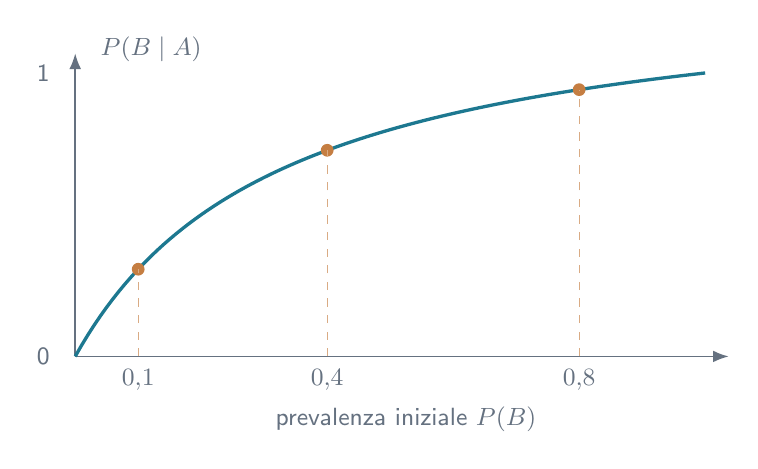
\begin{tikzpicture}[x=1cm,y=1cm]
\draw[pAxis](.6,.2)--(8.9,.2);\draw[pAxis](.6,.2)--(.6,4.05);
\draw[GeoA,line width=1.2pt] plot coordinates{(0.60000,0.20000) (0.68000,0.33981) (0.76000,0.47170) (0.84000,0.59633) (0.92000,0.71429) (1.00000,0.82609) (1.08000,0.93220) (1.16000,1.03306) (1.24000,1.12903) (1.32000,1.22047) (1.40000,1.30769) (1.48000,1.39098) (1.56000,1.47059) (1.64000,1.54676) (1.72000,1.61972) (1.80000,1.68966) (1.88000,1.75676) (1.96000,1.82119) (2.04000,1.88312) (2.12000,1.94268) (2.20000,2.00000) (2.28000,2.05521) (2.36000,2.10843) (2.44000,2.15976) (2.52000,2.20930) (2.60000,2.25714) (2.68000,2.30337) (2.76000,2.34807) (2.84000,2.39130) (2.92000,2.43316) (3.00000,2.47368) (3.08000,2.51295) (3.16000,2.55102) (3.24000,2.58794) (3.32000,2.62376) (3.40000,2.65854) (3.48000,2.69231) (3.56000,2.72512) (3.64000,2.75701) (3.72000,2.78802) (3.80000,2.81818) (3.88000,2.84753) (3.96000,2.87611) (4.04000,2.90393) (4.12000,2.93103) (4.20000,2.95745) (4.28000,2.98319) (4.36000,3.00830) (4.44000,3.03279) (4.52000,3.05668) (4.60000,3.08000) (4.68000,3.10277) (4.76000,3.12500) (4.84000,3.14672) (4.92000,3.16794) (5.00000,3.18868) (5.08000,3.20896) (5.16000,3.22878) (5.24000,3.24818) (5.32000,3.26715) (5.40000,3.28571) (5.48000,3.30389) (5.56000,3.32168) (5.64000,3.33910) (5.72000,3.35616) (5.80000,3.37288) (5.88000,3.38926) (5.96000,3.40532) (6.04000,3.42105) (6.12000,3.43648) (6.20000,3.45161) (6.28000,3.46645) (6.36000,3.48101) (6.44000,3.49530) (6.52000,3.50932) (6.60000,3.52308) (6.68000,3.53659) (6.76000,3.54985) (6.84000,3.56287) (6.92000,3.57567) (7.00000,3.58824) (7.08000,3.60058) (7.16000,3.61272) (7.24000,3.62464) (7.32000,3.63636) (7.40000,3.64789) (7.48000,3.65922) (7.56000,3.67036) (7.64000,3.68132) (7.72000,3.69210) (7.80000,3.70270) (7.88000,3.71314) (7.96000,3.72340) (8.04000,3.73351) (8.12000,3.74346) (8.20000,3.75325) (8.28000,3.76289) (8.36000,3.77238) (8.44000,3.78173) (8.52000,3.79093) (8.60000,3.80000)};
\foreach \x/\y/\lab in {1.4/1.30769/{0{,}1},3.8/2.81818/{0{,}4},7/3.58824/{0{,}8}}{
\fill[GeoB](\x,\y) circle(2.3pt);
\draw[GeoB!65,dashed](\x,.2)--(\x,\y);
\node[pNote] at(\x,-.1){$\lab$};}
\node[pNote,anchor=east] at(.4,.2){0};
\node[pNote,anchor=east] at(.4,3.8){1};
\node[pNote] at(4.8,-.6){prevalenza iniziale $P(B)$};
\node[pNote,anchor=west] at(.8,4.1){$P(B\mid A)$};
\end{tikzpicture}
\PSmall{La curva deriva direttamente da Bayes. I tre punti corrispondono ai valori calcolati nel codice.}

\end{minipage}% 
\end{lrbox}
\typeout{FULLBOX:014:L:\the\ht\PilotLeftBox:\the\dp\PilotLeftBox}
\begin{lrbox}{\PilotRightBox}%
\begin{minipage}[t]{7.55cm}\raggedright\color{Ink}\fontsize{11.3}{14.8}\selectfont

\PCode{R · modificare un solo parametro}{14_prevalenza.R}
\PBody{La quota $P(B\mid A)$ vale circa 0,308, 0,727 e 0,941 nei tre scenari.}
\PInfo{Trasferire un criterio di riconoscimento a un altro contesto richiede di riesaminare la composizione iniziale e la validità dei tassi condizionati.}

\end{minipage}% 
\end{lrbox}
\typeout{FULLBOX:014:R:\the\ht\PilotRightBox:\the\dp\PilotRightBox}
\begin{frame}[plain]\hypertarget{slide14}{}
\bookmark[level=1,page=14]{La composizione iniziale cambia il risultato}
\begin{tikzpicture}[remember picture,overlay]
\PilotChrome{La composizione iniziale cambia il risultato}{CONDIZIONAMENTO}{14}{A parità di probabilità condizionate, la quota del tipo B fra i segnali cambia con la prevalenza iniziale.}
\node[anchor=north west,inner sep=0] at ([xshift=0.96cm,yshift=-2.13cm]current page.north west) {\usebox{\PilotLeftBox}};
\node[anchor=north west,inner sep=0] at ([xshift=11.52cm,yshift=-2.13cm]current page.north west) {\usebox{\PilotRightBox}};

\end{tikzpicture}\end{frame}

% SLIDE 015 | Un classificatore su mille campioni
\begin{lrbox}{\PilotLeftBox}%
\begin{minipage}[t]{10.05cm}\raggedright\color{Ink}\fontsize{11.3}{14.8}\selectfont

\PLabel{Un secondo esempio costruito}
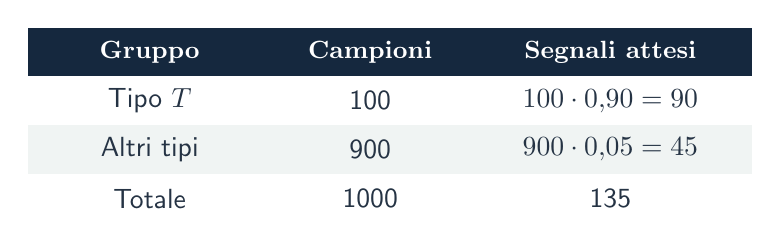
\begin{tikzpicture}[x=1cm,y=1cm]
\fill[Navy](0,0) rectangle(9.2,0.62);
\node[font=\bfseries\fontsize{9.5}{12}\selectfont,text=white] at(1.55,0.31){Gruppo};
\node[font=\bfseries\fontsize{9.5}{12}\selectfont,text=white] at(4.35,0.31){Campioni};
\node[font=\bfseries\fontsize{9.5}{12}\selectfont,text=white] at(7.3999999999999995,0.31){Segnali attesi};
\fill[white](0,-0.62) rectangle(9.2,0.0);
\node[pLabel] at(1.55,-0.31){Tipo $T$};
\node[pLabel] at(4.35,-0.31){100};
\node[pLabel] at(7.3999999999999995,-0.31){$100\cdot0{,}90=90$};
\fill[GeoTint](0,-1.24) rectangle(9.2,-0.62);
\node[pLabel] at(1.55,-0.9299999999999999){Altri tipi};
\node[pLabel] at(4.35,-0.9299999999999999){900};
\node[pLabel] at(7.3999999999999995,-0.9299999999999999){$900\cdot0{,}05=45$};
\fill[white](0,-1.8599999999999999) rectangle(9.2,-1.2399999999999998);
\node[pLabel] at(1.55,-1.5499999999999998){Totale};
\node[pLabel] at(4.35,-1.5499999999999998){1000};
\node[pLabel] at(7.3999999999999995,-1.5499999999999998){135};
\end{tikzpicture}
\vspace{4mm}
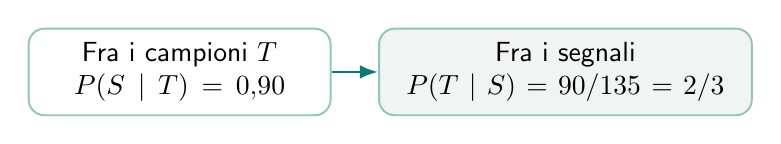
\begin{tikzpicture}[x=1cm,y=1cm]
\node[pFlow,text width=3.6cm] (a) at(2.05,.7){Fra i campioni $T$\\$P(S\mid T)=0{,}90$};
\node[pFlow,text width=4.5cm,fill=GeoTint] (b) at(6.95,.7){Fra i segnali\\$P(T\mid S)=90/135=2/3$};
\draw[pEdge](a)--(b);
\end{tikzpicture}
\PSmall{Il tipo $T$ e il segnale $S$ appartengono a questo nuovo scenario. I parametri differiscono da quelli predefiniti nel browser.}

\end{minipage}% 
\end{lrbox}
\typeout{FULLBOX:015:L:\the\ht\PilotLeftBox:\the\dp\PilotLeftBox}
\begin{lrbox}{\PilotRightBox}%
\begin{minipage}[t]{7.55cm}\raggedright\color{Ink}\fontsize{11.3}{14.8}\selectfont

\PCode{R · contare i segnali attesi}{15_mille_casi.R}
\PBody{Gli altri tipi sono nove volte più numerosi. La probabilità del 5\% produce 45 segnali attesi.}
\PInfo{I conteggi sono attesi. Un campione osservato può produrre numeri diversi.}

\end{minipage}% 
\end{lrbox}
\typeout{FULLBOX:015:R:\the\ht\PilotRightBox:\the\dp\PilotRightBox}
\begin{frame}[plain]\hypertarget{slide15}{}
\bookmark[level=1,page=15]{Un classificatore su mille campioni}
\begin{tikzpicture}[remember picture,overlay]
\PilotChrome{Un classificatore su mille campioni}{CONDIZIONAMENTO}{15}{Il significato di un segnale dipende anche dalla numerosità dei gruppi che possono produrlo.}
\node[anchor=north west,inner sep=0] at ([xshift=0.96cm,yshift=-2.13cm]current page.north west) {\usebox{\PilotLeftBox}};
\node[anchor=north west,inner sep=0] at ([xshift=11.52cm,yshift=-2.13cm]current page.north west) {\usebox{\PilotRightBox}};

\end{tikzpicture}\end{frame}

% SLIDE 016 | Laboratorio: marginali e condizionate
\begin{lrbox}{\PilotLeftBox}%
\begin{minipage}[t]{10.05cm}\raggedright\color{Ink}\fontsize{11.3}{14.8}\selectfont

\PLab{https://marzione00.github.io/Lab_Geo/\#laboratorio/m04-condizionamento}{Esperimento m04-condizionamento}
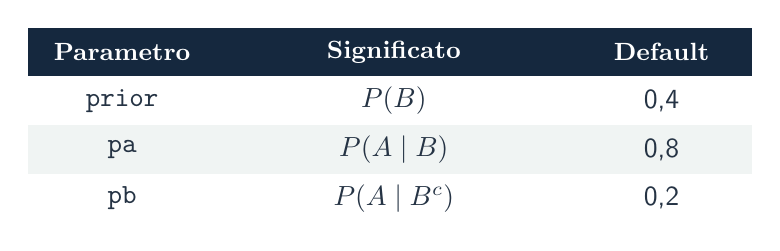
\begin{tikzpicture}[x=1cm,y=1cm]
\fill[Navy](0,0) rectangle(9.2,0.62);
\node[font=\bfseries\fontsize{9.5}{12}\selectfont,text=white] at(1.2,0.31){Parametro};
\node[font=\bfseries\fontsize{9.5}{12}\selectfont,text=white] at(4.65,0.31){Significato};
\node[font=\bfseries\fontsize{9.5}{12}\selectfont,text=white] at(8.05,0.31){Default};
\fill[white](0,-0.62) rectangle(9.2,0.0);
\node[pLabel] at(1.2,-0.31){\texttt{prior}};
\node[pLabel] at(4.65,-0.31){$P(B)$};
\node[pLabel] at(8.05,-0.31){0,4};
\fill[GeoTint](0,-1.24) rectangle(9.2,-0.62);
\node[pLabel] at(1.2,-0.9299999999999999){\texttt{pa}};
\node[pLabel] at(4.65,-0.9299999999999999){$P(A\mid B)$};
\node[pLabel] at(8.05,-0.9299999999999999){0,8};
\fill[white](0,-1.8599999999999999) rectangle(9.2,-1.2399999999999998);
\node[pLabel] at(1.2,-1.5499999999999998){\texttt{pb}};
\node[pLabel] at(4.65,-1.5499999999999998){$P(A\mid B^c)$};
\node[pLabel] at(8.05,-1.5499999999999998){0,2};
\end{tikzpicture}
\vspace{4mm}
\PBody{Prima diminuire \texttt{prior} mantenendo fissi gli altri parametri. Poi impostare \texttt{pa=pb} e controllare l'indipendenza.}
\PInfo{Annotare $P(A)$ e $P(B\mid A)$, spiegando perché rispondono in modo diverso al cambiamento dei parametri.}

\end{minipage}% 
\end{lrbox}
\typeout{FULLBOX:016:L:\the\ht\PilotLeftBox:\the\dp\PilotLeftBox}
\begin{lrbox}{\PilotRightBox}%
\begin{minipage}[t]{7.55cm}\raggedright\color{Ink}\fontsize{11.3}{14.8}\selectfont

\PCode{R · due confronti}{16_lab_condizionamento.R}
\PSmall{Il risultato è deterministico: deriva dalle formule. Il seme presente nell'interfaccia non modifica questo esperimento.}

\end{minipage}% 
\end{lrbox}
\typeout{FULLBOX:016:R:\the\ht\PilotRightBox:\the\dp\PilotRightBox}
\begin{frame}[plain]\hypertarget{slide16}{}
\bookmark[level=1,page=16]{Laboratorio: marginali e condizionate}
\begin{tikzpicture}[remember picture,overlay]
\PilotChrome{Laboratorio: marginali e condizionate}{LABORATORIO · CONDIZIONAMENTO}{16}{La marginale combina i gruppi; la probabilità inversa ripesa i gruppi fra i casi che soddisfano la condizione.}
\node[anchor=north west,inner sep=0] at ([xshift=0.96cm,yshift=-2.13cm]current page.north west) {\usebox{\PilotLeftBox}};
\node[anchor=north west,inner sep=0] at ([xshift=11.52cm,yshift=-2.13cm]current page.north west) {\usebox{\PilotRightBox}};

\end{tikzpicture}\end{frame}

% SLIDE 017 | Le condizioni della formula di Bayes
\begin{lrbox}{\PilotLeftBox}%
\begin{minipage}[t]{10.05cm}\raggedright\color{Ink}\fontsize{11.3}{14.8}\selectfont

\PLabel{Il calcolo richiede un modello coerente}
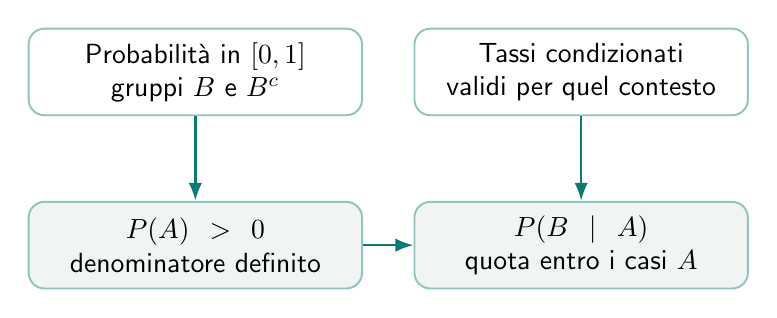
\begin{tikzpicture}[x=1cm,y=1cm]
\node[pFlow,text width=4cm] (a) at(2.2,3.3){Probabilità in $[0,1]$\\gruppi $B$ e $B^c$};
\node[pFlow,text width=4cm] (b) at(7.1,3.3){Tassi condizionati\\validi per quel contesto};
\node[pFlow,text width=4cm,fill=GeoTint] (c) at(2.2,1.1){$P(A)>0$\\denominatore definito};
\node[pFlow,text width=4cm,fill=GeoTint] (d) at(7.1,1.1){$P(B\mid A)$\\quota entro i casi $A$};
\draw[pEdge](a)--(c);\draw[pEdge](b)--(d);\draw[pEdge](c)--(d);
\end{tikzpicture}
\PBody{Se $A$ ha probabilità nulla, il rapporto usato qui non definisce $P(B\mid A)$. In R restituiamo \texttt{NA} per rendere visibile il problema.}

\end{minipage}% 
\end{lrbox}
\typeout{FULLBOX:017:L:\the\ht\PilotLeftBox:\the\dp\PilotLeftBox}
\begin{lrbox}{\PilotRightBox}%
\begin{minipage}[t]{7.55cm}\raggedright\color{Ink}\fontsize{11.3}{14.8}\selectfont

\PCode{R · una condizione non definita}{17_dominio.R}
\PSmall{La funzione è un esempio didattico con argomenti già validi in $[0,1]$. \texttt{NA\_real\_} rappresenta un valore numerico mancante.}
\PInfo{Il laboratorio limita i parametri a valori interni a $(0,1)$. Il caso con probabilità nulla serve a chiarire il dominio della formula.}

\end{minipage}% 
\end{lrbox}
\typeout{FULLBOX:017:R:\the\ht\PilotRightBox:\the\dp\PilotRightBox}
\begin{frame}[plain]\hypertarget{slide17}{}
\bookmark[level=1,page=17]{Le condizioni della formula di Bayes}
\begin{tikzpicture}[remember picture,overlay]
\PilotChrome{Le condizioni della formula di Bayes}{CONDIZIONAMENTO}{17}{Il valore numerico ha significato solo insieme al denominatore e alle ipotesi che definiscono il modello.}
\node[anchor=north west,inner sep=0] at ([xshift=0.96cm,yshift=-2.13cm]current page.north west) {\usebox{\PilotLeftBox}};
\node[anchor=north west,inner sep=0] at ([xshift=11.52cm,yshift=-2.13cm]current page.north west) {\usebox{\PilotRightBox}};

\end{tikzpicture}\end{frame}

% SLIDE 018 | Una variabile assegna numeri agli esiti
\begin{lrbox}{\PilotLeftBox}%
\begin{minipage}[t]{10.05cm}\raggedright\color{Ink}\fontsize{11.3}{14.8}\selectfont

\PLabel{$X:\Omega\longrightarrow\mathbb R$}
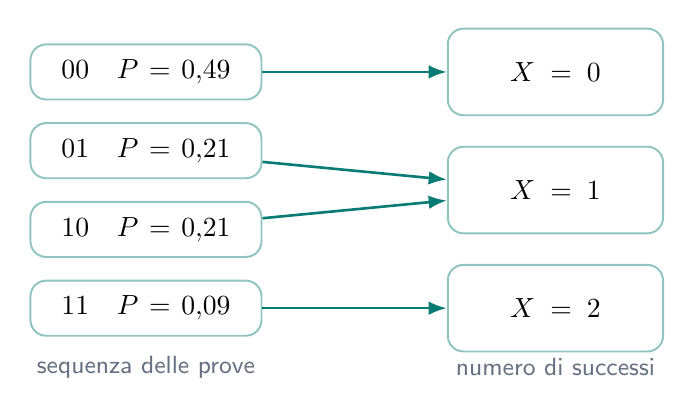
\begin{tikzpicture}[x=1cm,y=1cm]
\foreach \y/\lab/\p in {4/00/{0{,}49},3/01/{0{,}21},2/10/{0{,}21},1/11/{0{,}09}}{
\node[pFlow,minimum height=.7cm,text width=2.7cm] (s\lab) at(1.9,\y){$\lab\quad P=\p$};}
\node[pFlow,text width=2.5cm] (z) at(7.1,4){$X=0$};
\node[pFlow,text width=2.5cm] (u) at(7.1,2.5){$X=1$};
\node[pFlow,text width=2.5cm] (d) at(7.1,1){$X=2$};
\draw[pEdge](s00)--(z);\draw[pEdge](s01)--(u);\draw[pEdge](s10)--(u);\draw[pEdge](s11)--(d);
\node[pNote] at(1.9,.25){sequenza delle prove};
\node[pNote] at(7.1,.25){numero di successi};
\end{tikzpicture}
\PBody{Esiti diversi possono produrre lo stesso numero. La distribuzione di $X$ somma le probabilità degli esiti che portano a quel valore.}

\end{minipage}% 
\end{lrbox}
\typeout{FULLBOX:018:L:\the\ht\PilotLeftBox:\the\dp\PilotLeftBox}
\begin{lrbox}{\PilotRightBox}%
\begin{minipage}[t]{7.55cm}\raggedright\color{Ink}\fontsize{11.3}{14.8}\selectfont

\PCode{R · raggruppare gli esiti}{18_variabile.R}
\PSmall{Con prove indipendenti e $p=0{,}3$, la sequenza 01 pesa $0{,}7\cdot0{,}3=0{,}21$. Anche 10 pesa 0,21.}
\PInfo{Quindi $P(X=1)=0{,}21+0{,}21=0{,}42$. Il conteggio perde l'ordine delle due prove.}

\end{minipage}% 
\end{lrbox}
\typeout{FULLBOX:018:R:\the\ht\PilotRightBox:\the\dp\PilotRightBox}
\begin{frame}[plain]\hypertarget{slide18}{}
\bookmark[level=1,page=18]{Una variabile assegna numeri agli esiti}
\begin{tikzpicture}[remember picture,overlay]
\PilotChrome{Una variabile assegna numeri agli esiti}{VARIABILI E DISTRIBUZIONI}{18}{Una variabile casuale associa un numero a ciascun esito; la sua distribuzione trasferisce a quei numeri le probabilità.}
\node[anchor=north west,inner sep=0] at ([xshift=0.96cm,yshift=-2.13cm]current page.north west) {\usebox{\PilotLeftBox}};
\node[anchor=north west,inner sep=0] at ([xshift=11.52cm,yshift=-2.13cm]current page.north west) {\usebox{\PilotRightBox}};

\end{tikzpicture}\end{frame}

% SLIDE 019 | La massa di probabilità discreta
\begin{lrbox}{\PilotLeftBox}%
\begin{minipage}[t]{10.05cm}\raggedright\color{Ink}\fontsize{11.3}{14.8}\selectfont

\PLabel{$p_X(k)=P(X=k)$}
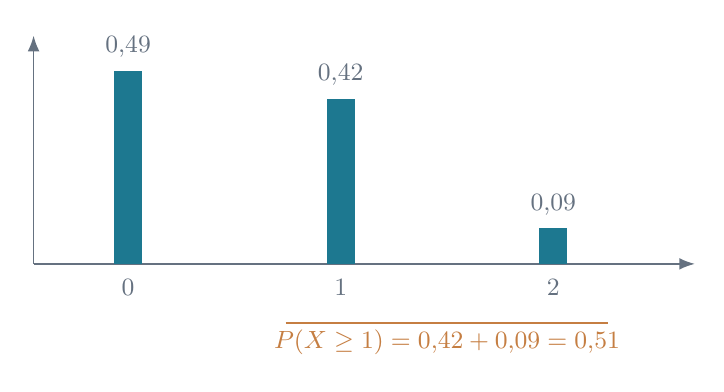
\begin{tikzpicture}[x=1cm,y=1cm]
\draw[pAxis](.4,.2)--(8.8,.2);\draw[pAxis](.4,.2)--(.4,3.1);
\foreach \x/\y/\p/\k in {1.6/2.65/{0{,}49}/0,4.3/2.3/{0{,}42}/1,7/.65/{0{,}09}/2}{
\draw[GeoA,line width=10pt](\x,.2)--(\x,\y);
\node[pNote] at(\x,\y+.3){$\p$};\node[pNote] at(\x,-.1){$\k$};}
\draw[GeoB,line width=1pt](3.6,-.55)--(7.7,-.55);
\node[pNote,text=GeoB] at(5.65,-.8){$P(X\ge1)=0{,}42+0{,}09=0{,}51$};
\end{tikzpicture}
\[
p_X(k)\ge0,\qquad \sum_k p_X(k)=1.
\]
\PSmall{Le barre rappresentano le masse sui valori possibili. Le probabilità degli eventi si ottengono sommando.}

\end{minipage}% 
\end{lrbox}
\typeout{FULLBOX:019:L:\the\ht\PilotLeftBox:\the\dp\PilotLeftBox}
\begin{lrbox}{\PilotRightBox}%
\begin{minipage}[t]{7.55cm}\raggedright\color{Ink}\fontsize{11.3}{14.8}\selectfont

\PCode{R · sommare le masse}{19_massa.R}
\PSmall{\texttt{k19>=1} seleziona i valori inclusi nell'evento. Le masse sono pesi del modello e sommano a uno.}
\PInfo{La media teorica vale 0,6 successi. Una singola osservazione di $X$ può valere solo 0, 1 o 2.}

\end{minipage}% 
\end{lrbox}
\typeout{FULLBOX:019:R:\the\ht\PilotRightBox:\the\dp\PilotRightBox}
\begin{frame}[plain]\hypertarget{slide19}{}
\bookmark[level=1,page=19]{La massa di probabilità discreta}
\begin{tikzpicture}[remember picture,overlay]
\PilotChrome{La massa di probabilità discreta}{VARIABILI E DISTRIBUZIONI}{19}{Per una variabile discreta, le probabilità dei singoli valori sono masse che si sommano.}
\node[anchor=north west,inner sep=0] at ([xshift=0.96cm,yshift=-2.13cm]current page.north west) {\usebox{\PilotLeftBox}};
\node[anchor=north west,inner sep=0] at ([xshift=11.52cm,yshift=-2.13cm]current page.north west) {\usebox{\PilotRightBox}};

\end{tikzpicture}\end{frame}

% SLIDE 020 | La probabilità continua è un’area
\begin{lrbox}{\PilotLeftBox}%
\begin{minipage}[t]{10.05cm}\raggedright\color{Ink}\fontsize{11.3}{14.8}\selectfont

\PLabel{Una variabile uniforme su $[0,2]$, adimensionale}
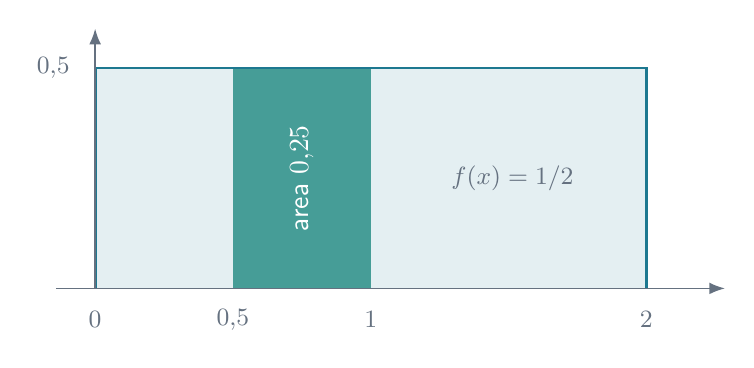
\begin{tikzpicture}[x=1cm,y=1cm]
\fill[GeoA!12](1,.3) rectangle(8,3.1);
\fill[Classical!75](2.75,.3) rectangle(4.5,3.1);
\draw[GeoA,line width=1pt](1,.3)--(1,3.1)--(8,3.1)--(8,.3);
\draw[pAxis](.5,.3)--(9,.3);\draw[pAxis](1,.3)--(1,3.6);
\foreach \x/\lab in {1/0,2.75/{0{,}5},4.5/1,8/2}{\node[pNote] at(\x,-.1){$\lab$};}
\node[pNote,anchor=east] at(.8,3.1){$0{,}5$};
\node[pLabel,text=white,rotate=90] at(3.625,1.7){area $0{,}25$};
\node[pNote] at(6.3,1.7){$f(x)=1/2$};
\end{tikzpicture}
\[
P(0{,}5<X\le1)=\int_{0{,}5}^{1}\tfrac12\,dx=0{,}25.
\]
\PSmall{La larghezza dell'intervallo è 0,5. L'altezza della densità è 0,5. Il prodotto restituisce la probabilità.}

\end{minipage}% 
\end{lrbox}
\typeout{FULLBOX:020:L:\the\ht\PilotLeftBox:\the\dp\PilotLeftBox}
\begin{lrbox}{\PilotRightBox}%
\begin{minipage}[t]{7.55cm}\raggedright\color{Ink}\fontsize{11.3}{14.8}\selectfont

\PCode{R · densità e cumulata}{20_densita.R}
\PSmall{\texttt{dunif()} restituisce l'altezza. \texttt{punif()} restituisce la probabilità cumulata fino alla soglia.}
\PInfo{Per una distribuzione con densità, $P(X=x)=0$ per ogni singolo punto. Le probabilità riguardano intervalli o insiemi di valori.}

\end{minipage}% 
\end{lrbox}
\typeout{FULLBOX:020:R:\the\ht\PilotRightBox:\the\dp\PilotRightBox}
\begin{frame}[plain]\hypertarget{slide20}{}
\bookmark[level=1,page=20]{La probabilità continua è un’area}
\begin{tikzpicture}[remember picture,overlay]
\PilotChrome{La probabilità continua è un’area}{VARIABILI E DISTRIBUZIONI}{20}{L’altezza della densità e la probabilità hanno significati diversi: la probabilità continua si calcola integrando.}
\node[anchor=north west,inner sep=0] at ([xshift=0.96cm,yshift=-2.13cm]current page.north west) {\usebox{\PilotLeftBox}};
\node[anchor=north west,inner sep=0] at ([xshift=11.52cm,yshift=-2.13cm]current page.north west) {\usebox{\PilotRightBox}};

\end{tikzpicture}\end{frame}

% SLIDE 021 | Una densità può superare uno
\begin{lrbox}{\PilotLeftBox}%
\begin{minipage}[t]{10.05cm}\raggedright\color{Ink}\fontsize{11.3}{14.8}\selectfont

\PLabel{Uniforme su un intervallo più stretto}
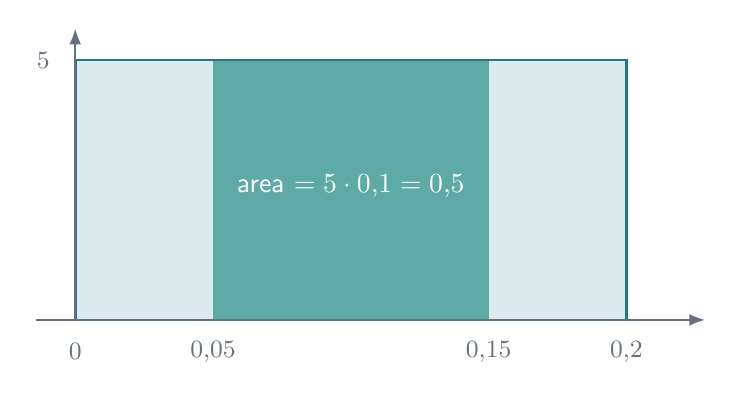
\begin{tikzpicture}[x=1cm,y=1cm]
\fill[GeoA!15](1,.3) rectangle(8,3.6);
\fill[Classical!65](2.75,.3) rectangle(6.25,3.6);
\draw[GeoA,line width=1pt](1,.3)--(1,3.6)--(8,3.6)--(8,.3);
\draw[pAxis](.5,.3)--(9,.3);\draw[pAxis](1,.3)--(1,4);
\foreach \x/\lab in {1/0,2.75/{0{,}05},6.25/{0{,}15},8/{0{,}2}}{\node[pNote] at(\x,-.1){$\lab$};}
\node[pNote,anchor=east] at(.8,3.6){$5$};
\node[pLabel,text=white] at(4.5,2){area $=5\cdot0{,}1=0{,}5$};
\end{tikzpicture}
\[
\int_0^{0{,}2}5\,dx=1.
\]
\PSmall{Il vincolo $[0,1]$ riguarda la probabilità. Se $X$ ha un'unità fisica, la densità ha l'unità inversa.}

\end{minipage}% 
\end{lrbox}
\typeout{FULLBOX:021:L:\the\ht\PilotLeftBox:\the\dp\PilotLeftBox}
\begin{lrbox}{\PilotRightBox}%
\begin{minipage}[t]{7.55cm}\raggedright\color{Ink}\fontsize{11.3}{14.8}\selectfont

\PCode{R · un’altezza pari a cinque}{21_altezza.R}
\PBody{Accorciare il supporto dell'uniforme aumenta l'altezza necessaria a conservare area totale uno.}
\PInfo{Il valore letto su un asse di densità richiede anche la scala e l'unità della variabile. La probabilità resta adimensionale.}

\end{minipage}% 
\end{lrbox}
\typeout{FULLBOX:021:R:\the\ht\PilotRightBox:\the\dp\PilotRightBox}
\begin{frame}[plain]\hypertarget{slide21}{}
\bookmark[level=1,page=21]{Una densità può superare uno}
\begin{tikzpicture}[remember picture,overlay]
\PilotChrome{Una densità può superare uno}{VARIABILI E DISTRIBUZIONI}{21}{Una densità alta è compatibile con una probabilità totale pari a uno quando il supporto è sufficientemente stretto.}
\node[anchor=north west,inner sep=0] at ([xshift=0.96cm,yshift=-2.13cm]current page.north west) {\usebox{\PilotLeftBox}};
\node[anchor=north west,inner sep=0] at ([xshift=11.52cm,yshift=-2.13cm]current page.north west) {\usebox{\PilotRightBox}};

\end{tikzpicture}\end{frame}

% SLIDE 022 | La funzione di distribuzione cumulativa
\begin{lrbox}{\PilotLeftBox}%
\begin{minipage}[t]{10.05cm}\raggedright\color{Ink}\fontsize{11.3}{14.8}\selectfont

\PLabel{$F_X(x)=P(X\le x)$}
\begin{tikzpicture}[x=1cm,y=1cm]
\draw[pAxis](.5,.2)--(9,.2);\draw[pAxis](.5,.2)--(.5,3.9);
\draw[GeoA,line width=1.1pt](.5,.2)--(1.5,.2);
\draw[GeoA,line width=1.1pt](1.5,1.866)--(4.2,1.866);
\draw[GeoA,line width=1.1pt](4.2,3.294)--(6.9,3.294);
\draw[GeoA,line width=1.1pt](6.9,3.6)--(8.7,3.6);
\foreach \x/\y in {1.5/1.866,4.2/3.294,6.9/3.6}{\fill[GeoA](\x,\y) circle(2.3pt);}
\foreach \x/\y in {1.5/.2,4.2/1.866,6.9/3.294}{\draw[GeoA,fill=Paper](\x,\y) circle(2.3pt);}
\foreach \x/\lab in {1.5/0,4.2/1,6.9/2}{\node[pNote] at(\x,-.1){\lab};}
\foreach \y/\lab in {1.866/{0{,}49},3.294/{0{,}91},3.6/1}{\node[pNote,anchor=east] at(.3,\y){$\lab$};}
\node[pNote] at(4.8,-.55){soglia $x$};
\end{tikzpicture}
\PSmall{Nel modello discreto, il salto in $k$ ha ampiezza $P(X=k)$. La cumulativa è non decrescente e comprende il valore alla soglia.}
\[
P(a<X\le b)=F_X(b)-F_X(a).
\]

\end{minipage}% 
\end{lrbox}
\typeout{FULLBOX:022:L:\the\ht\PilotLeftBox:\the\dp\PilotLeftBox}
\begin{lrbox}{\PilotRightBox}%
\begin{minipage}[t]{7.55cm}\raggedright\color{Ink}\fontsize{11.3}{14.8}\selectfont

\PCode{R · accumulare le probabilità}{22_cumulativa.R}
\PSmall{Per la variabile discreta delle pagine precedenti, $F(1)=0{,}49+0{,}42=0{,}91$.}
\PInfo{La differenza di cumulative vale anche nel continuo. Nel discreto occorre leggere con attenzione gli estremi inclusi ed esclusi.}

\end{minipage}% 
\end{lrbox}
\typeout{FULLBOX:022:R:\the\ht\PilotRightBox:\the\dp\PilotRightBox}
\begin{frame}[plain]\hypertarget{slide22}{}
\bookmark[level=1,page=22]{La funzione di distribuzione cumulativa}
\begin{tikzpicture}[remember picture,overlay]
\PilotChrome{La funzione di distribuzione cumulativa}{VARIABILI E DISTRIBUZIONI}{22}{La cumulativa raccoglie tutta la probabilità fino alla soglia, compresa la massa eventualmente presente sulla soglia.}
\node[anchor=north west,inner sep=0] at ([xshift=0.96cm,yshift=-2.13cm]current page.north west) {\usebox{\PilotLeftBox}};
\node[anchor=north west,inner sep=0] at ([xshift=11.52cm,yshift=-2.13cm]current page.north west) {\usebox{\PilotRightBox}};

\end{tikzpicture}\end{frame}

% SLIDE 023 | Media e varianza del modello
\begin{lrbox}{\PilotLeftBox}%
\begin{minipage}[t]{10.05cm}\raggedright\color{Ink}\fontsize{11.3}{14.8}\selectfont

\PLabel{Il centro e gli scarti pesati dalle probabilità}
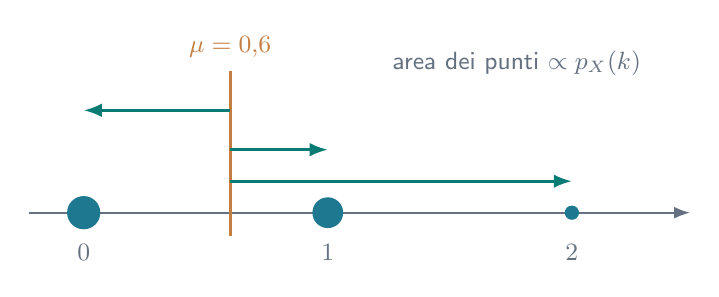
\begin{tikzpicture}[x=1cm,y=1cm]
\draw[pAxis](.6,1.2)--(9,1.2);
\foreach \x/\k/\sz in {1.3/0/6,4.4/1/5.555,7.5/2/2.5714}{
\fill[GeoA](\x,1.2) circle(\sz pt);\node[pNote] at(\x,.7){$\k$};}
\draw[GeoB,line width=1pt](3.16,.9)--(3.16,3);
\node[pNote,text=GeoB] at(3.16,3.3){$\mu=0{,}6$};
\draw[pEdge](3.16,2.5)--(1.3,2.5);
\draw[pEdge](3.16,2.0)--(4.4,2.0);
\draw[pEdge](3.16,1.6)--(7.5,1.6);
\node[pNote] at(6.8,3.1){area dei punti $\propto p_X(k)$};
\end{tikzpicture}
\[
\mu=\mathbb E[X],\qquad
\sigma^2=\mathbb E[(X-\mu)^2],\qquad
\sigma=\sqrt{\sigma^2}.
\]
\PSmall{Nel continuo, le somme pesate diventano integrali contro la densità. Queste quantità richiedono momenti finiti.}

\end{minipage}% 
\end{lrbox}
\typeout{FULLBOX:023:L:\the\ht\PilotLeftBox:\the\dp\PilotLeftBox}
\begin{lrbox}{\PilotRightBox}%
\begin{minipage}[t]{7.55cm}\raggedright\color{Ink}\fontsize{11.3}{14.8}\selectfont

\PCode{R · momenti teorici}{23_momenti.R}
\PSmall{I pesi sommano a uno. La formula è quella del modello e non usa il divisore campionario $n-1$.}
\PInfo{Se $X$ è una lunghezza in mm, $\sigma$ è in mm e $\sigma^2$ in mm$^2$. Media e deviazione standard conservano l'unità originale.}

\end{minipage}% 
\end{lrbox}
\typeout{FULLBOX:023:R:\the\ht\PilotRightBox:\the\dp\PilotRightBox}
\begin{frame}[plain]\hypertarget{slide23}{}
\bookmark[level=1,page=23]{Media e varianza del modello}
\begin{tikzpicture}[remember picture,overlay]
\PilotChrome{Media e varianza del modello}{VARIABILI E DISTRIBUZIONI}{23}{Media e varianza del modello usano le probabilità; le statistiche campionarie usano le osservazioni disponibili.}
\node[anchor=north west,inner sep=0] at ([xshift=0.96cm,yshift=-2.13cm]current page.north west) {\usebox{\PilotLeftBox}};
\node[anchor=north west,inner sep=0] at ([xshift=11.52cm,yshift=-2.13cm]current page.north west) {\usebox{\PilotRightBox}};

\end{tikzpicture}\end{frame}

% SLIDE 024 | Il quantile inverte la cumulativa
\begin{lrbox}{\PilotLeftBox}%
\begin{minipage}[t]{10.05cm}\raggedright\color{Ink}\fontsize{11.3}{14.8}\selectfont

\PLabel{La soglia che raggiunge una probabilità assegnata}
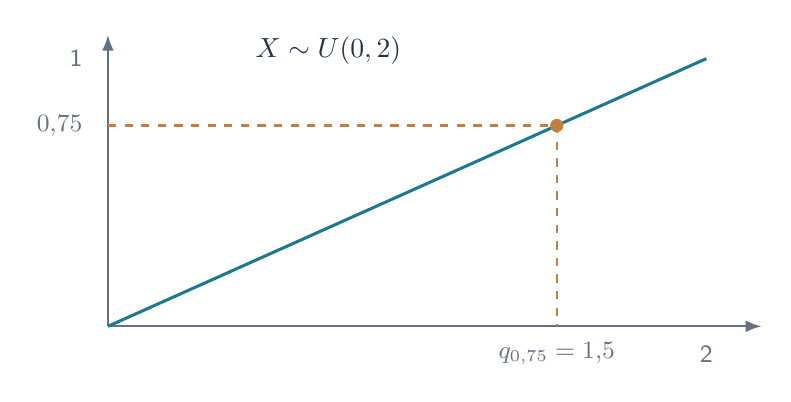
\begin{tikzpicture}[x=1cm,y=1cm]
\draw[pAxis](.7,.3)--(9,.3);\draw[pAxis](.7,.3)--(.7,4);
\draw[GeoA,line width=1.1pt](.7,.3)--(8.3,3.7);
\draw[GeoB,dashed,line width=.9pt](.7,2.85)--(6.4,2.85)--(6.4,.3);
\node[pNote,anchor=east] at(.5,2.85){$0{,}75$};
\node[pNote] at(6.4,-.05){$q_{0{,}75}=1{,}5$};
\node[pNote] at(8.3,-.05){2};
\node[pNote,anchor=east] at(.5,3.7){1};
\node[pLabel] at(3.5,3.8){$X\sim U(0,2)$};
\fill[GeoB](6.4,2.85) circle(2.4pt);
\end{tikzpicture}
\[
q_\alpha=\inf\{x:F_X(x)\ge\alpha\},\quad0<\alpha<1.
\]
\PSmall{Per il discreto, il quantile è il primo valore che raggiunge o supera $\alpha$. L'uguaglianza $F(q_\alpha)=\alpha$ può fallire.}

\end{minipage}% 
\end{lrbox}
\typeout{FULLBOX:024:L:\the\ht\PilotLeftBox:\the\dp\PilotLeftBox}
\begin{lrbox}{\PilotRightBox}%
\begin{minipage}[t]{7.55cm}\raggedright\color{Ink}\fontsize{11.3}{14.8}\selectfont

\PCode{R · dal livello alla soglia}{24_quantile.R}
\PSmall{\texttt{qunif()} lavora sul modello uniforme. \texttt{quantile(x)} calcola invece quantili da un vettore di dati, con una convenzione di interpolazione.}
\PInfo{Nel caso discreto, $q_{0{,}75}=1$ perché $F(0)=0{,}49<0{,}75$ e $F(1)=0{,}91\ge0{,}75$.}

\end{minipage}% 
\end{lrbox}
\typeout{FULLBOX:024:R:\the\ht\PilotRightBox:\the\dp\PilotRightBox}
\begin{frame}[plain]\hypertarget{slide24}{}
\bookmark[level=1,page=24]{Il quantile inverte la cumulativa}
\begin{tikzpicture}[remember picture,overlay]
\PilotChrome{Il quantile inverte la cumulativa}{VARIABILI E DISTRIBUZIONI}{24}{Il quantile risponde alla domanda inversa: quale soglia raccoglie almeno la probabilità richiesta?}
\node[anchor=north west,inner sep=0] at ([xshift=0.96cm,yshift=-2.13cm]current page.north west) {\usebox{\PilotLeftBox}};
\node[anchor=north west,inner sep=0] at ([xshift=11.52cm,yshift=-2.13cm]current page.north west) {\usebox{\PilotRightBox}};

\end{tikzpicture}\end{frame}

% SLIDE 025 | Laboratorio: soglia, area e cumulata
\begin{lrbox}{\PilotLeftBox}%
\begin{minipage}[t]{10.05cm}\raggedright\color{Ink}\fontsize{11.3}{14.8}\selectfont

\PLab{https://marzione00.github.io/Lab_Geo/\#laboratorio/m04-distribuzione}{Esperimento m04-distribuzione}
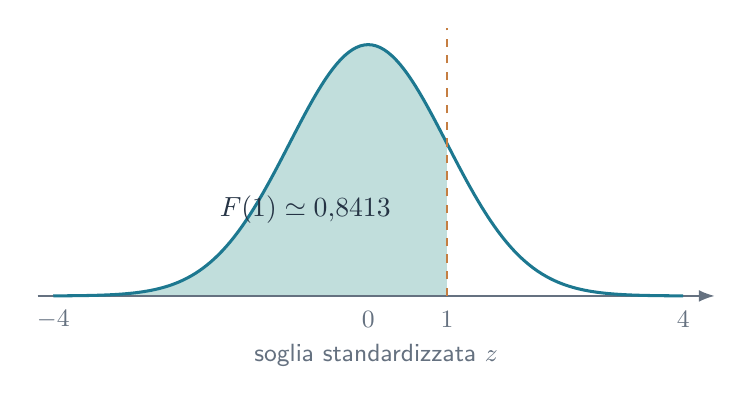
\begin{tikzpicture}[x=1cm,y=1cm]
\fill[Classical!25](.6,.2)--(0.60000,0.20107) -- (0.65000,0.20131) -- (0.70000,0.20159) -- (0.75000,0.20193) -- (0.80000,0.20234) -- (0.85000,0.20282) -- (0.90000,0.20340) -- (0.95000,0.20408) -- (1.00000,0.20490) -- (1.05000,0.20585) -- (1.10000,0.20698) -- (1.15000,0.20831) -- (1.20000,0.20986) -- (1.25000,0.21167) -- (1.30000,0.21378) -- (1.35000,0.21623) -- (1.40000,0.21907) -- (1.45000,0.22235) -- (1.50000,0.22613) -- (1.55000,0.23048) -- (1.60000,0.23545) -- (1.65000,0.24114) -- (1.70000,0.24762) -- (1.75000,0.25498) -- (1.80000,0.26332) -- (1.85000,0.27275) -- (1.90000,0.28337) -- (1.95000,0.29530) -- (2.00000,0.30866) -- (2.05000,0.32359) -- (2.10000,0.34023) -- (2.15000,0.35870) -- (2.20000,0.37916) -- (2.25000,0.40175) -- (2.30000,0.42662) -- (2.35000,0.45392) -- (2.40000,0.48380) -- (2.45000,0.51640) -- (2.50000,0.55187) -- (2.55000,0.59034) -- (2.60000,0.63193) -- (2.65000,0.67676) -- (2.70000,0.72493) -- (2.75000,0.77652) -- (2.80000,0.83160) -- (2.85000,0.89022) -- (2.90000,0.95239) -- (2.95000,1.01812) -- (3.00000,1.08737) -- (3.05000,1.16007) -- (3.10000,1.23614) -- (3.15000,1.31544) -- (3.20000,1.39782) -- (3.25000,1.48307) -- (3.30000,1.57095) -- (3.35000,1.66119) -- (3.40000,1.75349) -- (3.45000,1.84749) -- (3.50000,1.94282) -- (3.55000,2.03906) -- (3.60000,2.13577) -- (3.65000,2.23247) -- (3.70000,2.32868) -- (3.75000,2.42388) -- (3.80000,2.51753) -- (3.85000,2.60910) -- (3.90000,2.69803) -- (3.95000,2.78378) -- (4.00000,2.86580) -- (4.05000,2.94355) -- (4.10000,3.01652) -- (4.15000,3.08422) -- (4.20000,3.14616) -- (4.25000,3.20192) -- (4.30000,3.25110) -- (4.35000,3.29334) -- (4.40000,3.32834) -- (4.45000,3.35583) -- (4.50000,3.37562) -- (4.55000,3.38755) -- (4.60000,3.39154) -- (4.65000,3.38755) -- (4.70000,3.37562) -- (4.75000,3.35583) -- (4.80000,3.32834) -- (4.85000,3.29334) -- (4.90000,3.25110) -- (4.95000,3.20192) -- (5.00000,3.14616) -- (5.05000,3.08422) -- (5.10000,3.01652) -- (5.15000,2.94355) -- (5.20000,2.86580) -- (5.25000,2.78378) -- (5.30000,2.69803) -- (5.35000,2.60910) -- (5.40000,2.51753) -- (5.45000,2.42388) -- (5.50000,2.32868) -- (5.55000,2.23247) -- (5.60000,2.13577)--(5.6,.2)--cycle;
\draw[pAxis](.4,.2)--(9,.2);
\draw[GeoA,line width=1.1pt] plot coordinates{(0.60000,0.20107) (0.65000,0.20131) (0.70000,0.20159) (0.75000,0.20193) (0.80000,0.20234) (0.85000,0.20282) (0.90000,0.20340) (0.95000,0.20408) (1.00000,0.20490) (1.05000,0.20585) (1.10000,0.20698) (1.15000,0.20831) (1.20000,0.20986) (1.25000,0.21167) (1.30000,0.21378) (1.35000,0.21623) (1.40000,0.21907) (1.45000,0.22235) (1.50000,0.22613) (1.55000,0.23048) (1.60000,0.23545) (1.65000,0.24114) (1.70000,0.24762) (1.75000,0.25498) (1.80000,0.26332) (1.85000,0.27275) (1.90000,0.28337) (1.95000,0.29530) (2.00000,0.30866) (2.05000,0.32359) (2.10000,0.34023) (2.15000,0.35870) (2.20000,0.37916) (2.25000,0.40175) (2.30000,0.42662) (2.35000,0.45392) (2.40000,0.48380) (2.45000,0.51640) (2.50000,0.55187) (2.55000,0.59034) (2.60000,0.63193) (2.65000,0.67676) (2.70000,0.72493) (2.75000,0.77652) (2.80000,0.83160) (2.85000,0.89022) (2.90000,0.95239) (2.95000,1.01812) (3.00000,1.08737) (3.05000,1.16007) (3.10000,1.23614) (3.15000,1.31544) (3.20000,1.39782) (3.25000,1.48307) (3.30000,1.57095) (3.35000,1.66119) (3.40000,1.75349) (3.45000,1.84749) (3.50000,1.94282) (3.55000,2.03906) (3.60000,2.13577) (3.65000,2.23247) (3.70000,2.32868) (3.75000,2.42388) (3.80000,2.51753) (3.85000,2.60910) (3.90000,2.69803) (3.95000,2.78378) (4.00000,2.86580) (4.05000,2.94355) (4.10000,3.01652) (4.15000,3.08422) (4.20000,3.14616) (4.25000,3.20192) (4.30000,3.25110) (4.35000,3.29334) (4.40000,3.32834) (4.45000,3.35583) (4.50000,3.37562) (4.55000,3.38755) (4.60000,3.39154) (4.65000,3.38755) (4.70000,3.37562) (4.75000,3.35583) (4.80000,3.32834) (4.85000,3.29334) (4.90000,3.25110) (4.95000,3.20192) (5.00000,3.14616) (5.05000,3.08422) (5.10000,3.01652) (5.15000,2.94355) (5.20000,2.86580) (5.25000,2.78378) (5.30000,2.69803) (5.35000,2.60910) (5.40000,2.51753) (5.45000,2.42388) (5.50000,2.32868) (5.55000,2.23247) (5.60000,2.13577) (5.65000,2.03906) (5.70000,1.94282) (5.75000,1.84749) (5.80000,1.75349) (5.85000,1.66119) (5.90000,1.57095) (5.95000,1.48307) (6.00000,1.39782) (6.05000,1.31544) (6.10000,1.23614) (6.15000,1.16007) (6.20000,1.08737) (6.25000,1.01812) (6.30000,0.95239) (6.35000,0.89022) (6.40000,0.83160) (6.45000,0.77652) (6.50000,0.72493) (6.55000,0.67676) (6.60000,0.63193) (6.65000,0.59034) (6.70000,0.55187) (6.75000,0.51640) (6.80000,0.48380) (6.85000,0.45392) (6.90000,0.42662) (6.95000,0.40175) (7.00000,0.37916) (7.05000,0.35870) (7.10000,0.34023) (7.15000,0.32359) (7.20000,0.30866) (7.25000,0.29530) (7.30000,0.28337) (7.35000,0.27275) (7.40000,0.26332) (7.45000,0.25498) (7.50000,0.24762) (7.55000,0.24114) (7.60000,0.23545) (7.65000,0.23048) (7.70000,0.22613) (7.75000,0.22235) (7.80000,0.21907) (7.85000,0.21623) (7.90000,0.21378) (7.95000,0.21167) (8.00000,0.20986) (8.05000,0.20831) (8.10000,0.20698) (8.15000,0.20585) (8.20000,0.20490) (8.25000,0.20408) (8.30000,0.20340) (8.35000,0.20282) (8.40000,0.20234) (8.45000,0.20193) (8.50000,0.20159) (8.55000,0.20131) (8.60000,0.20107)};
\draw[GeoB,dashed](5.6,.2)--(5.6,3.6);
\foreach \x/\lab in {.6/{-4},4.6/0,5.6/1,8.6/4}{\node[pNote] at(\x,-.1){$\lab$};}
\node[pLabel] at(3.8,1.3){$F(1)\simeq0{,}8413$};
\node[pNote] at(4.7,-.55){soglia standardizzata $z$};
\end{tikzpicture}
\PBody{Spostare la soglia modifica l'area cumulata, mentre la curva della normale standard rimane la stessa.}
\PSmall{Il disegno mostra $[-4,4]$. Gli indicatori usano \texttt{pnorm()} sull'intera distribuzione, comprese le code esterne al grafico.}

\end{minipage}% 
\end{lrbox}
\typeout{FULLBOX:025:L:\the\ht\PilotLeftBox:\the\dp\PilotLeftBox}
\begin{lrbox}{\PilotRightBox}%
\begin{minipage}[t]{7.55cm}\raggedright\color{Ink}\fontsize{11.3}{14.8}\selectfont

\PCode{R · cumulata e superamento}{25_lab_distribuzione.R}
\PSmall{\texttt{lower.tail=FALSE} restituisce $P(Z>z)$. La cumulata e il superamento sommano a uno.}
\PInfo{Il calcolo è deterministico. La normale standard sarà studiata nel blocco dedicato a posizione, scala e quantili.}

\end{minipage}% 
\end{lrbox}
\typeout{FULLBOX:025:R:\the\ht\PilotRightBox:\the\dp\PilotRightBox}
\begin{frame}[plain]\hypertarget{slide25}{}
\bookmark[level=1,page=25]{Laboratorio: soglia, area e cumulata}
\begin{tikzpicture}[remember picture,overlay]
\PilotChrome{Laboratorio: soglia, area e cumulata}{LABORATORIO · DISTRIBUZIONE}{25}{La soglia determina una probabilità cumulata; il taglio grafico delle code non cambia il calcolo analitico.}
\node[anchor=north west,inner sep=0] at ([xshift=0.96cm,yshift=-2.13cm]current page.north west) {\usebox{\PilotLeftBox}};
\node[anchor=north west,inner sep=0] at ([xshift=11.52cm,yshift=-2.13cm]current page.north west) {\usebox{\PilotRightBox}};

\end{tikzpicture}\end{frame}

% SLIDE 026 | Una prova, due esiti: Bernoulli
\begin{lrbox}{\PilotLeftBox}%
\begin{minipage}[t]{10.05cm}\raggedright\color{Ink}\fontsize{11.3}{14.8}\selectfont

\PLabel{Un indicatore assegna 1 all'evento e 0 al complemento}
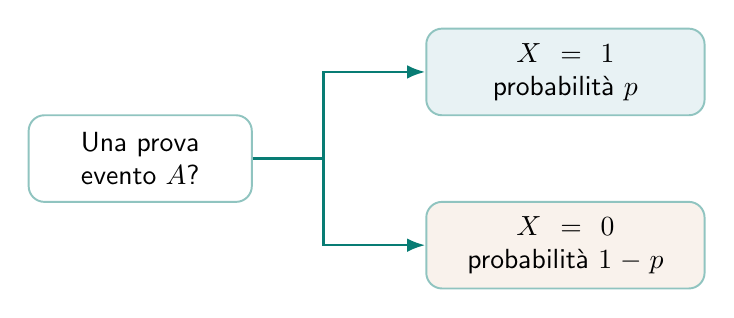
\begin{tikzpicture}[x=1cm,y=1cm]
\node[pFlow,text width=2.6cm] (a) at(1.6,1.65){Una prova\\evento $A$?};
\node[pFlow,text width=3.3cm,fill=GeoA!10] (b) at(7,2.75){$X=1$\\probabilità $p$};
\node[pFlow,text width=3.3cm,fill=GeoB!10] (c) at(7,.55){$X=0$\\probabilità $1-p$};
\draw[pEdge](a.east)--++(.9,0)|-(b.west);
\draw[pEdge](a.east)--++(.9,0)|-(c.west);
\end{tikzpicture}
\[
X\sim\operatorname{Bern}(p),\quad
\operatorname E[X]=p,\quad
\operatorname{Var}(X)=p(1-p).
\]
\PSmall{$0\le p\le1$. Un esempio: rilevare una frattura in un provino secondo un criterio fissato prima dell'osservazione.}

\end{minipage}% 
\end{lrbox}
\typeout{FULLBOX:026:L:\the\ht\PilotLeftBox:\the\dp\PilotLeftBox}
\begin{lrbox}{\PilotRightBox}%
\begin{minipage}[t]{7.55cm}\raggedright\color{Ink}\fontsize{11.3}{14.8}\selectfont

\PCode{R · simulare indicatori}{26_bernoulli.R}
\PSmall{In \texttt{rbinom()}, \texttt{size=1} indica una sola prova per valore. Il primo argomento chiede 12 valori simulati.}
\PInfo{La media del modello è $p$. La frequenza ottenuta in una breve simulazione può discostarsene.}

\end{minipage}% 
\end{lrbox}
\typeout{FULLBOX:026:R:\the\ht\PilotRightBox:\the\dp\PilotRightBox}
\begin{frame}[plain]\hypertarget{slide26}{}
\bookmark[level=1,page=26]{Una prova, due esiti: Bernoulli}
\begin{tikzpicture}[remember picture,overlay]
\PilotChrome{Una prova, due esiti: Bernoulli}{BERNOULLI E BINOMIALE}{26}{Bernoulli descrive un singolo evento binario. Il parametro p è la probabilità assegnata all’esito 1.}
\node[anchor=north west,inner sep=0] at ([xshift=0.96cm,yshift=-2.13cm]current page.north west) {\usebox{\PilotLeftBox}};
\node[anchor=north west,inner sep=0] at ([xshift=11.52cm,yshift=-2.13cm]current page.north west) {\usebox{\PilotRightBox}};

\end{tikzpicture}\end{frame}

% SLIDE 027 | Dalle prove al numero di successi
\begin{lrbox}{\PilotLeftBox}%
\begin{minipage}[t]{10.05cm}\raggedright\color{Ink}\fontsize{11.3}{14.8}\selectfont

\PLabel{Esempio costruito: 20 provini, 6 positivi}
\begin{tikzpicture}[x=1cm,y=1cm]
\foreach \i/\v in {0/1,1/0,2/0,3/1,4/0,5/0,6/1,7/0,8/0,9/0,
10/1,11/0,12/0,13/0,14/1,15/0,16/0,17/1,18/0,19/0}{
\pgfmathtruncatemacro{\row}{int(\i/10)}
\pgfmathtruncatemacro{\col}{mod(\i,10)}
\ifnum\v=1\relax
\node[draw=GeoA,fill=GeoA!16,minimum size=.65cm,pLabel] at(.5+.9*\col,2.3-1.0*\row){\v};
\else
\node[draw=Rule,fill=white,minimum size=.65cm,pLabel] at(.5+.9*\col,2.3-1.0*\row){\v};
\fi
}
\node[pNote] at(4.55,.35){Ogni casella è una prova; ogni 1 contribuisce al conteggio.};
\end{tikzpicture}
\[
K=\sum_{i=1}^{n}X_i,\qquad K\in\{0,1,\ldots,n\}.
\]
\PBody{Con $n$ prove indipendenti e la stessa probabilità $p$, il conteggio $K$ segue una distribuzione binomiale.}

\end{minipage}% 
\end{lrbox}
\typeout{FULLBOX:027:L:\the\ht\PilotLeftBox:\the\dp\PilotLeftBox}
\begin{lrbox}{\PilotRightBox}%
\begin{minipage}[t]{7.55cm}\raggedright\color{Ink}\fontsize{11.3}{14.8}\selectfont

\PCode{R · prove, conteggio, proporzione}{27_somma_prove.R}
\PInfo{Tre quantità: $n=20$ prove; $K=6$ successi nella sequenza; $K/n=0{,}30$ come proporzione osservata.}
\PSmall{Il numero di prove si fissa prima. Un campionamento senza reinserimento da una piccola popolazione richiede un modello diverso.}

\end{minipage}% 
\end{lrbox}
\typeout{FULLBOX:027:R:\the\ht\PilotRightBox:\the\dp\PilotRightBox}
\begin{frame}[plain]\hypertarget{slide27}{}
\bookmark[level=1,page=27]{Dalle prove al numero di successi}
\begin{tikzpicture}[remember picture,overlay]
\PilotChrome{Dalle prove al numero di successi}{BERNOULLI E BINOMIALE}{27}{La binomiale conta i successi in un numero fissato di prove indipendenti con probabilità comune.}
\node[anchor=north west,inner sep=0] at ([xshift=0.96cm,yshift=-2.13cm]current page.north west) {\usebox{\PilotLeftBox}};
\node[anchor=north west,inner sep=0] at ([xshift=11.52cm,yshift=-2.13cm]current page.north west) {\usebox{\PilotRightBox}};

\end{tikzpicture}\end{frame}

% SLIDE 028 | La formula conta tutte le sequenze possibili
\begin{lrbox}{\PilotLeftBox}%
\begin{minipage}[t]{10.05cm}\raggedright\color{Ink}\fontsize{11.3}{14.8}\selectfont

\PLabel{Tre modi per ottenere due successi su tre prove}
\begin{tikzpicture}[x=1cm,y=1cm]
\foreach \y/\a/\b/\c in {2.65/1/1/0,1.65/1/0/1,.65/0/1/1}{
\node[pFlow,minimum width=.8cm,minimum height=.65cm] at(.8,\y){\a};
\node[pFlow,minimum width=.8cm,minimum height=.65cm] at(2.1,\y){\b};
\node[pFlow,minimum width=.8cm,minimum height=.65cm] at(3.4,\y){\c};
\draw[pEdge](4,\y)--(5.2,\y);
\node[pLabel,anchor=west] at(5.4,\y){probabilità $p^2(1-p)$};
}
\end{tikzpicture}
\[
P(K=k)=\binom nk p^k(1-p)^{n-k}.
\]
\PSmall{$\binom nk$ conta le posizioni dei $k$ successi. L'indipendenza consente di moltiplicare le probabilità delle singole prove.}

\end{minipage}% 
\end{lrbox}
\typeout{FULLBOX:028:L:\the\ht\PilotLeftBox:\the\dp\PilotLeftBox}
\begin{lrbox}{\PilotRightBox}%
\begin{minipage}[t]{7.55cm}\raggedright\color{Ink}\fontsize{11.3}{14.8}\selectfont

\PCode{R · formula e funzione}{28_probabilita_binomiale.R}
\PSmall{\texttt{choose(n,k)} calcola il coefficiente binomiale. \texttt{dbinom()} restituisce la probabilità del singolo conteggio indicato.}
\PInfo{Per $n=20$, $p=0{,}3$: $P(K=8)\simeq0{,}1144$. La probabilità di \emph{almeno} 8 comprende altri conteggi.}

\end{minipage}% 
\end{lrbox}
\typeout{FULLBOX:028:R:\the\ht\PilotRightBox:\the\dp\PilotRightBox}
\begin{frame}[plain]\hypertarget{slide28}{}
\bookmark[level=1,page=28]{La formula conta tutte le sequenze possibili}
\begin{tikzpicture}[remember picture,overlay]
\PilotChrome{La formula conta tutte le sequenze possibili}{BERNOULLI E BINOMIALE}{28}{La probabilità di un conteggio somma quelle di tutte le sequenze che producono lo stesso numero di successi.}
\node[anchor=north west,inner sep=0] at ([xshift=0.96cm,yshift=-2.13cm]current page.north west) {\usebox{\PilotLeftBox}};
\node[anchor=north west,inner sep=0] at ([xshift=11.52cm,yshift=-2.13cm]current page.north west) {\usebox{\PilotRightBox}};

\end{tikzpicture}\end{frame}

% SLIDE 029 | Media e dispersione del conteggio
\begin{lrbox}{\PilotLeftBox}%
\begin{minipage}[t]{10.05cm}\raggedright\color{Ink}\fontsize{11.3}{14.8}\selectfont

\PLabel{Distribuzione teorica: $n=20$, $p=0{,}3$}
\begin{tikzpicture}[x=1cm,y=1cm]
\draw[Rule] (.85,0.0000)--(8.85,0.0000);
\node[pNote,anchor=east] at (.7,0.0000) {0};
\draw[Rule] (.85,1.1136)--(8.85,1.1136);
\node[pNote,anchor=east] at (.7,1.1136) {0{,}1};
\draw[Rule] (.85,2.2273)--(8.85,2.2273);
\node[pNote,anchor=east] at (.7,2.2273) {0{,}2};
\draw[pAxis] (.85,0)--(9.05,0);
\draw[pAxis] (.85,0)--(.85,2.6300000000000003);
\draw[Muted] (1.0764,0)--(1.0764,-.08);\node[pNote,below] at (1.0764,-.1) {0};
\draw[Muted] (2.9632,0)--(2.9632,-.08);\node[pNote,below] at (2.9632,-.1) {5};
\draw[Muted] (4.8500,0)--(4.8500,-.08);\node[pNote,below] at (4.8500,-.1) {10};
\draw[Muted] (6.7368,0)--(6.7368,-.08);\node[pNote,below] at (6.7368,-.1) {15};
\draw[Muted] (8.6236,0)--(8.6236,-.08);\node[pNote,below] at (8.6236,-.1) {20};
\node[pNote] at (4.85,-.65) {$k$: numero di eventi};
\node[pNote,rotate=90] at (-.18,1.225) {$P(K=k)$};
\draw[GeoA,line width=2pt] (1.0764,0)--(1.0764,0.0089);
\draw[GeoA,line width=2pt] (1.4538,0)--(1.4538,0.0762);
\draw[GeoA,line width=2pt] (1.8311,0)--(1.8311,0.3101);
\draw[GeoA,line width=2pt] (2.2085,0)--(2.2085,0.7974);
\draw[GeoA,line width=2pt] (2.5858,0)--(2.5858,1.4524);
\draw[GeoA,line width=2pt] (2.9632,0)--(2.9632,1.9919);
\draw[GeoA,line width=2pt] (3.3406,0)--(3.3406,2.1342);
\draw[GeoA,line width=2pt] (3.7179,0)--(3.7179,1.8293);
\draw[GeoA,line width=2pt] (4.0953,0)--(4.0953,1.2740);
\draw[GeoA,line width=2pt] (4.4726,0)--(4.4726,0.7280);
\draw[GeoA,line width=2pt] (4.8500,0)--(4.8500,0.3432);
\draw[GeoA,line width=2pt] (5.2274,0)--(5.2274,0.1337);
\draw[GeoA,line width=2pt] (5.6047,0)--(5.6047,0.0430);
\draw[GeoA,line width=2pt] (5.9821,0)--(5.9821,0.0113);
\draw[GeoA,line width=2pt] (6.3594,0)--(6.3594,0.0024);
\draw[GeoA,line width=2pt] (6.7368,0)--(6.7368,0.0004);
\draw[GeoA,line width=2pt] (7.1142,0)--(7.1142,0.0001);
\draw[GeoA,line width=2pt] (7.4915,0)--(7.4915,0.0000);
\draw[GeoA,line width=2pt] (7.8689,0)--(7.8689,0.0000);
\draw[GeoA,line width=2pt] (8.2462,0)--(8.2462,0.0000);
\draw[GeoA,line width=2pt] (8.6236,0)--(8.6236,0.0000);
\node[pNote,anchor=north east] at (8.9,2.5) {$E[K]=6$};
\end{tikzpicture}
\[
\operatorname E[K]=np=6,\qquad
\operatorname{Var}(K)=np(1-p)=4{,}2.
\]
\PSmall{La deviazione standard è $\sqrt{4{,}2}\simeq2{,}05$ successi. La media teorica può essere non intera anche se ogni conteggio è intero.}

\end{minipage}% 
\end{lrbox}
\typeout{FULLBOX:029:L:\the\ht\PilotLeftBox:\the\dp\PilotLeftBox}
\begin{lrbox}{\PilotRightBox}%
\begin{minipage}[t]{7.55cm}\raggedright\color{Ink}\fontsize{11.3}{14.8}\selectfont

\PCode{R · momenti del modello}{29_centro_dispersione.R}
\PSmall{Il prodotto \texttt{k29 * dbinom(...)} pesa ogni conteggio con la sua probabilità. La somma ricostruisce la media teorica.}

\end{minipage}% 
\end{lrbox}
\typeout{FULLBOX:029:R:\the\ht\PilotRightBox:\the\dp\PilotRightBox}
\begin{frame}[plain]\hypertarget{slide29}{}
\bookmark[level=1,page=29]{Media e dispersione del conteggio}
\begin{tikzpicture}[remember picture,overlay]
\PilotChrome{Media e dispersione del conteggio}{BERNOULLI E BINOMIALE}{29}{Per la binomiale la media vale np e la varianza np(1−p). Descrivono la distribuzione dei conteggi.}
\node[anchor=north west,inner sep=0] at ([xshift=0.96cm,yshift=-2.13cm]current page.north west) {\usebox{\PilotLeftBox}};
\node[anchor=north west,inner sep=0] at ([xshift=11.52cm,yshift=-2.13cm]current page.north west) {\usebox{\PilotRightBox}};

\end{tikzpicture}\end{frame}

% SLIDE 030 | «Almeno 8» comprende 8, 9, 10, …
\begin{lrbox}{\PilotLeftBox}%
\begin{minipage}[t]{10.05cm}\raggedright\color{Ink}\fontsize{11.3}{14.8}\selectfont

\PLabel{La coda discreta inizia dal valore incluso}
\begin{tikzpicture}[x=1cm,y=1cm]
\draw[Rule] (.85,0.0000)--(8.85,0.0000);
\node[pNote,anchor=east] at (.7,0.0000) {0};
\draw[Rule] (.85,1.1136)--(8.85,1.1136);
\node[pNote,anchor=east] at (.7,1.1136) {0{,}1};
\draw[Rule] (.85,2.2273)--(8.85,2.2273);
\node[pNote,anchor=east] at (.7,2.2273) {0{,}2};
\draw[pAxis] (.85,0)--(9.05,0);
\draw[pAxis] (.85,0)--(.85,2.6300000000000003);
\draw[Muted] (1.0764,0)--(1.0764,-.08);\node[pNote,below] at (1.0764,-.1) {0};
\draw[Muted] (2.9632,0)--(2.9632,-.08);\node[pNote,below] at (2.9632,-.1) {5};
\draw[Muted] (4.8500,0)--(4.8500,-.08);\node[pNote,below] at (4.8500,-.1) {10};
\draw[Muted] (6.7368,0)--(6.7368,-.08);\node[pNote,below] at (6.7368,-.1) {15};
\draw[Muted] (8.6236,0)--(8.6236,-.08);\node[pNote,below] at (8.6236,-.1) {20};
\node[pNote] at (4.85,-.65) {$k$: numero di eventi};
\node[pNote,rotate=90] at (-.18,1.225) {$P(K=k)$};
\draw[GeoA,line width=2pt] (1.0764,0)--(1.0764,0.0089);
\draw[GeoA,line width=2pt] (1.4538,0)--(1.4538,0.0762);
\draw[GeoA,line width=2pt] (1.8311,0)--(1.8311,0.3101);
\draw[GeoA,line width=2pt] (2.2085,0)--(2.2085,0.7974);
\draw[GeoA,line width=2pt] (2.5858,0)--(2.5858,1.4524);
\draw[GeoA,line width=2pt] (2.9632,0)--(2.9632,1.9919);
\draw[GeoA,line width=2pt] (3.3406,0)--(3.3406,2.1342);
\draw[GeoA,line width=2pt] (3.7179,0)--(3.7179,1.8293);
\draw[GeoB,line width=2pt] (4.0953,0)--(4.0953,1.2740);
\draw[GeoB,line width=2pt] (4.4726,0)--(4.4726,0.7280);
\draw[GeoB,line width=2pt] (4.8500,0)--(4.8500,0.3432);
\draw[GeoB,line width=2pt] (5.2274,0)--(5.2274,0.1337);
\draw[GeoB,line width=2pt] (5.6047,0)--(5.6047,0.0430);
\draw[GeoB,line width=2pt] (5.9821,0)--(5.9821,0.0113);
\draw[GeoB,line width=2pt] (6.3594,0)--(6.3594,0.0024);
\draw[GeoB,line width=2pt] (6.7368,0)--(6.7368,0.0004);
\draw[GeoB,line width=2pt] (7.1142,0)--(7.1142,0.0001);
\draw[GeoB,line width=2pt] (7.4915,0)--(7.4915,0.0000);
\draw[GeoB,line width=2pt] (7.8689,0)--(7.8689,0.0000);
\draw[GeoB,line width=2pt] (8.2462,0)--(8.2462,0.0000);
\draw[GeoB,line width=2pt] (8.6236,0)--(8.6236,0.0000);
\node[pNote,anchor=north east] at (8.9,2.5) {arancio: $K\ge8$};
\end{tikzpicture}
\[
P(K\ge8)=1-P(K\le7)\simeq0{,}2277.
\]
\PBody{Con conteggi interi, $K\ge8$ equivale a $K>7$. Scrivere prima l'evento evita di spostare la soglia di una unità.}

\end{minipage}% 
\end{lrbox}
\typeout{FULLBOX:030:L:\the\ht\PilotLeftBox:\the\dp\PilotLeftBox}
\begin{lrbox}{\PilotRightBox}%
\begin{minipage}[t]{7.55cm}\raggedright\color{Ink}\fontsize{11.3}{14.8}\selectfont

\PCode{R · due calcoli equivalenti}{30_coda_binomiale.R}
\PInfo{\texttt{pbinom(8,...,lower.tail=FALSE)} calcolerebbe $P(K>8)$, escludendo il caso $K=8$.}
\PSmall{Le barre rappresentano masse di probabilità su valori interi; la probabilità di un insieme è la loro somma.}

\end{minipage}% 
\end{lrbox}
\typeout{FULLBOX:030:R:\the\ht\PilotRightBox:\the\dp\PilotRightBox}
\begin{frame}[plain]\hypertarget{slide30}{}
\bookmark[level=1,page=30]{«Almeno 8» comprende 8, 9, 10, …}
\begin{tikzpicture}[remember picture,overlay]
\PilotChrome{«Almeno 8» comprende 8, 9, 10, …}{BERNOULLI E BINOMIALE}{30}{Le disuguaglianze strette e inclusive producono risultati diversi per una variabile discreta.}
\node[anchor=north west,inner sep=0] at ([xshift=0.96cm,yshift=-2.13cm]current page.north west) {\usebox{\PilotLeftBox}};
\node[anchor=north west,inner sep=0] at ([xshift=11.52cm,yshift=-2.13cm]current page.north west) {\usebox{\PilotRightBox}};

\end{tikzpicture}\end{frame}

% SLIDE 031 | Quattro prefissi, quattro domande
\begin{lrbox}{\PilotLeftBox}%
\begin{minipage}[t]{10.05cm}\raggedright\color{Ink}\fontsize{11.3}{14.8}\selectfont

\PLabel{Stessi prefissi nelle diverse distribuzioni}
\begin{tikzpicture}[x=1cm,y=1cm]
\fill[GeoTint] (0,0) rectangle (9.4,0.68);
\node[font=\fontsize{9.8}{12.1}\selectfont,text=Ink,anchor=west] at (0.12,0.34) {Prefisso};
\node[font=\fontsize{9.8}{12.1}\selectfont,text=Ink,anchor=west] at (1.7200000000000002,0.34) {Domanda};
\node[font=\fontsize{9.8}{12.1}\selectfont,text=Ink,anchor=west] at (6.420000000000001,0.34) {Risultato};
\draw[Rule] (0,0.0)--(9.4,0.0);
\node[font=\fontsize{9.8}{12.1}\selectfont,text=Ink,anchor=west] at (0.12,-0.34) {\texttt{d}};
\node[font=\fontsize{9.8}{12.1}\selectfont,text=Ink,anchor=west] at (1.7200000000000002,-0.34) {$P(K=8)$};
\node[font=\fontsize{9.8}{12.1}\selectfont,text=Ink,anchor=west] at (6.420000000000001,-0.34) {una probabilità};
\draw[Rule] (0,-0.68)--(9.4,-0.68);
\node[font=\fontsize{9.8}{12.1}\selectfont,text=Ink,anchor=west] at (0.12,-1.02) {\texttt{p}};
\node[font=\fontsize{9.8}{12.1}\selectfont,text=Ink,anchor=west] at (1.7200000000000002,-1.02) {$P(K\le8)$};
\node[font=\fontsize{9.8}{12.1}\selectfont,text=Ink,anchor=west] at (6.420000000000001,-1.02) {una cumulata};
\draw[Rule] (0,-1.36)--(9.4,-1.36);
\node[font=\fontsize{9.8}{12.1}\selectfont,text=Ink,anchor=west] at (0.12,-1.7) {\texttt{q}};
\node[font=\fontsize{9.8}{12.1}\selectfont,text=Ink,anchor=west] at (1.7200000000000002,-1.7) {quale soglia per $0{,}95$?};
\node[font=\fontsize{9.8}{12.1}\selectfont,text=Ink,anchor=west] at (6.420000000000001,-1.7) {un conteggio};
\draw[Rule] (0,-2.04)--(9.4,-2.04);
\node[font=\fontsize{9.8}{12.1}\selectfont,text=Ink,anchor=west] at (0.12,-2.3800000000000003) {\texttt{r}};
\node[font=\fontsize{9.8}{12.1}\selectfont,text=Ink,anchor=west] at (1.7200000000000002,-2.3800000000000003) {quali esiti simulati?};
\node[font=\fontsize{9.8}{12.1}\selectfont,text=Ink,anchor=west] at (6.420000000000001,-2.3800000000000003) {un vettore};
\draw[Rule] (0,-2.72)--(9.4,-2.72);
\end{tikzpicture}
\vspace{3mm}
\[
q_\alpha=\min\{k:F_K(k)\ge\alpha\}.
\]
\PSmall{Per $K\sim\operatorname{Bin}(20,0{,}3)$, $q_{0,95}=9$. La cumulata a 9 supera $0{,}95$: i salti discreti impediscono di ottenere ogni livello esatto.}

\end{minipage}% 
\end{lrbox}
\typeout{FULLBOX:031:L:\the\ht\PilotLeftBox:\the\dp\PilotLeftBox}
\begin{lrbox}{\PilotRightBox}%
\begin{minipage}[t]{7.55cm}\raggedright\color{Ink}\fontsize{11.3}{14.8}\selectfont

\PCode{R · d, p, q, r}{31_quattro_funzioni.R}
\PSmall{In \texttt{rbinom(5,size=20,...)}, 5 è il numero di conteggi richiesti; ogni conteggio deriva da 20 prove.}

\end{minipage}% 
\end{lrbox}
\typeout{FULLBOX:031:R:\the\ht\PilotRightBox:\the\dp\PilotRightBox}
\begin{frame}[plain]\hypertarget{slide31}{}
\bookmark[level=1,page=31]{Quattro prefissi, quattro domande}
\begin{tikzpicture}[remember picture,overlay]
\PilotChrome{Quattro prefissi, quattro domande}{BERNOULLI E BINOMIALE}{31}{d restituisce una massa o densità, p una cumulata, q una soglia e r valori simulati.}
\node[anchor=north west,inner sep=0] at ([xshift=0.96cm,yshift=-2.13cm]current page.north west) {\usebox{\PilotLeftBox}};
\node[anchor=north west,inner sep=0] at ([xshift=11.52cm,yshift=-2.13cm]current page.north west) {\usebox{\PilotRightBox}};

\end{tikzpicture}\end{frame}

% SLIDE 032 | 400 repliche approssimano la distribuzione
\begin{lrbox}{\PilotLeftBox}%
\begin{minipage}[t]{10.05cm}\raggedright\color{Ink}\fontsize{11.3}{14.8}\selectfont

\PLabel{Stesso modello, frequenze ottenute con seme 17}
\begin{tikzpicture}[x=1cm,y=1cm]
\draw[Rule] (.85,0.0000)--(8.85,0.0000);
\node[pNote,anchor=east] at (.7,0.0000) {0};
\draw[Rule] (.85,1.1136)--(8.85,1.1136);
\node[pNote,anchor=east] at (.7,1.1136) {0{,}1};
\draw[Rule] (.85,2.2273)--(8.85,2.2273);
\node[pNote,anchor=east] at (.7,2.2273) {0{,}2};
\draw[pAxis] (.85,0)--(9.05,0);
\draw[pAxis] (.85,0)--(.85,2.6300000000000003);
\draw[Muted] (1.0764,0)--(1.0764,-.08);\node[pNote,below] at (1.0764,-.1) {0};
\draw[Muted] (2.9632,0)--(2.9632,-.08);\node[pNote,below] at (2.9632,-.1) {5};
\draw[Muted] (4.8500,0)--(4.8500,-.08);\node[pNote,below] at (4.8500,-.1) {10};
\draw[Muted] (6.7368,0)--(6.7368,-.08);\node[pNote,below] at (6.7368,-.1) {15};
\draw[Muted] (8.6236,0)--(8.6236,-.08);\node[pNote,below] at (8.6236,-.1) {20};
\node[pNote] at (4.85,-.65) {$k$: numero di eventi};
\node[pNote,rotate=90] at (-.18,1.225) {$P(K=k)$};
\draw[GeoA,line width=2pt] (1.0764,0)--(1.0764,0.0089);
\draw[GeoA,line width=2pt] (1.4538,0)--(1.4538,0.0762);
\draw[GeoA,line width=2pt] (1.8311,0)--(1.8311,0.3101);
\draw[GeoA,line width=2pt] (2.2085,0)--(2.2085,0.7974);
\draw[GeoA,line width=2pt] (2.5858,0)--(2.5858,1.4524);
\draw[GeoA,line width=2pt] (2.9632,0)--(2.9632,1.9919);
\draw[GeoA,line width=2pt] (3.3406,0)--(3.3406,2.1342);
\draw[GeoA,line width=2pt] (3.7179,0)--(3.7179,1.8293);
\draw[GeoA,line width=2pt] (4.0953,0)--(4.0953,1.2740);
\draw[GeoA,line width=2pt] (4.4726,0)--(4.4726,0.7280);
\draw[GeoA,line width=2pt] (4.8500,0)--(4.8500,0.3432);
\draw[GeoA,line width=2pt] (5.2274,0)--(5.2274,0.1337);
\draw[GeoA,line width=2pt] (5.6047,0)--(5.6047,0.0430);
\draw[GeoA,line width=2pt] (5.9821,0)--(5.9821,0.0113);
\draw[GeoA,line width=2pt] (6.3594,0)--(6.3594,0.0024);
\draw[GeoA,line width=2pt] (6.7368,0)--(6.7368,0.0004);
\draw[GeoA,line width=2pt] (7.1142,0)--(7.1142,0.0001);
\draw[GeoA,line width=2pt] (7.4915,0)--(7.4915,0.0000);
\draw[GeoA,line width=2pt] (7.8689,0)--(7.8689,0.0000);
\draw[GeoA,line width=2pt] (8.2462,0)--(8.2462,0.0000);
\draw[GeoA,line width=2pt] (8.6236,0)--(8.6236,0.0000);
\fill[GeoB] (1.0764,0.0557) circle(2.3pt);
\fill[GeoB] (1.4538,0.0835) circle(2.3pt);
\fill[GeoB] (1.8311,0.3063) circle(2.3pt);
\fill[GeoB] (2.2085,0.7517) circle(2.3pt);
\fill[GeoB] (2.5858,1.6983) circle(2.3pt);
\fill[GeoB] (2.9632,1.8932) circle(2.3pt);
\fill[GeoB] (3.3406,1.9489) circle(2.3pt);
\fill[GeoB] (3.7179,1.8932) circle(2.3pt);
\fill[GeoB] (4.0953,1.3642) circle(2.3pt);
\fill[GeoB] (4.4726,0.5568) circle(2.3pt);
\fill[GeoB] (4.8500,0.4176) circle(2.3pt);
\fill[GeoB] (5.2274,0.1392) circle(2.3pt);
\fill[GeoB] (5.6047,0.0278) circle(2.3pt);
\fill[GeoB] (5.9821,0.0000) circle(2.3pt);
\fill[GeoB] (6.3594,0.0000) circle(2.3pt);
\fill[GeoB] (6.7368,0.0000) circle(2.3pt);
\fill[GeoB] (7.1142,0.0000) circle(2.3pt);
\fill[GeoB] (7.4915,0.0000) circle(2.3pt);
\fill[GeoB] (7.8689,0.0000) circle(2.3pt);
\fill[GeoB] (8.2462,0.0000) circle(2.3pt);
\fill[GeoB] (8.6236,0.0000) circle(2.3pt);
\node[pNote,anchor=north east] at (8.9,2.5) {barre: teoria\\punti: frequenze};
\end{tikzpicture}
\PBody{Ogni replica genera un conteggio su $n=20$ prove. Le $B=400$ repliche costruiscono la distribuzione empirica dei conteggi.}
\PSmall{Con questo seme la media simulata è $5{,}9375$; quella teorica è 6. Le differenze dipendono dalla simulazione finita.}

\end{minipage}% 
\end{lrbox}
\typeout{FULLBOX:032:L:\the\ht\PilotLeftBox:\the\dp\PilotLeftBox}
\begin{lrbox}{\PilotRightBox}%
\begin{minipage}[t]{7.55cm}\raggedright\color{Ink}\fontsize{11.3}{14.8}\selectfont

\PCode{R · teoria e frequenze}{32_teoria_simulazione.R}
\PSmall{\texttt{tabulate(s32+1)} conta gli esiti: lo spostamento di 1 permette di includere il conteggio zero nella prima posizione.}

\end{minipage}% 
\end{lrbox}
\typeout{FULLBOX:032:R:\the\ht\PilotRightBox:\the\dp\PilotRightBox}
\begin{frame}[plain]\hypertarget{slide32}{}
\bookmark[level=1,page=32]{400 repliche approssimano la distribuzione}
\begin{tikzpicture}[remember picture,overlay]
\PilotChrome{400 repliche approssimano la distribuzione}{BERNOULLI E BINOMIALE}{32}{n indica le prove di una replica; B indica quante volte si ripete l’esperimento completo.}
\node[anchor=north west,inner sep=0] at ([xshift=0.96cm,yshift=-2.13cm]current page.north west) {\usebox{\PilotLeftBox}};
\node[anchor=north west,inner sep=0] at ([xshift=11.52cm,yshift=-2.13cm]current page.north west) {\usebox{\PilotRightBox}};

\end{tikzpicture}\end{frame}

% SLIDE 033 | Laboratorio: aumentare il numero di prove
\begin{lrbox}{\PilotLeftBox}%
\begin{minipage}[t]{10.05cm}\raggedright\color{Ink}\fontsize{11.3}{14.8}\selectfont

\PLabel{Esperimento m04-binomiale}
\begin{tikzpicture}[x=1cm,y=1cm]
\node[pFlow,text width=3.75cm] (a) at(2.2,2.5){$n=20,\ p=0{,}3$\\$E[K]=6$\\$\operatorname{Var}(K)=4{,}2$};
\node[pFlow,text width=3.75cm] (b) at(7.2,2.5){$n=40,\ p=0{,}3$\\$E[K]=12$\\$\operatorname{Var}(K)=8{,}4$};
\draw[pEdge](a)--node[pNote,above] {$n\times2$}(b);
\node[pLabel,text width=8.6cm] at(4.7,.55){Per la proporzione: $\operatorname{Var}(K/n)=p(1-p)/n$.};
\end{tikzpicture}
\PBody{Confrontare posizione e dispersione dei conteggi. Poi ripetere il confronto sulla proporzione $K/n$.}
\PSmall{Nel sito il numero di repliche rimane 400. \href{https://marzione00.github.io/Lab_Geo/\#laboratorio/m04-binomiale}{Aprire l'esperimento}.}

\end{minipage}% 
\end{lrbox}
\typeout{FULLBOX:033:L:\the\ht\PilotLeftBox:\the\dp\PilotLeftBox}
\begin{lrbox}{\PilotRightBox}%
\begin{minipage}[t]{7.55cm}\raggedright\color{Ink}\fontsize{11.3}{14.8}\selectfont

\PCode{R · due valori di n}{33_lab_binomiale.R}
\PInfo{Prima di eseguire: prevedere che cosa accade a media e deviazione standard di $K$, poi a quelle di $K/n$.}
\PSmall{Registrare parametri, previsione e risultato. Uno scarto della media simulata dalla teoria è atteso con repliche finite.}

\end{minipage}% 
\end{lrbox}
\typeout{FULLBOX:033:R:\the\ht\PilotRightBox:\the\dp\PilotRightBox}
\begin{frame}[plain]\hypertarget{slide33}{}
\bookmark[level=1,page=33]{Laboratorio: aumentare il numero di prove}
\begin{tikzpicture}[remember picture,overlay]
\PilotChrome{Laboratorio: aumentare il numero di prove}{BERNOULLI E BINOMIALE}{33}{Aumentare n amplia i conteggi possibili e riduce la dispersione della proporzione K/n, a p fissata.}
\node[anchor=north west,inner sep=0] at ([xshift=0.96cm,yshift=-2.13cm]current page.north west) {\usebox{\PilotLeftBox}};
\node[anchor=north west,inner sep=0] at ([xshift=11.52cm,yshift=-2.13cm]current page.north west) {\usebox{\PilotRightBox}};

\end{tikzpicture}\end{frame}

% SLIDE 034 | Poisson: tasso ed esposizione
\begin{lrbox}{\PilotLeftBox}%
\begin{minipage}[t]{10.05cm}\raggedright\color{Ink}\fontsize{11.3}{14.8}\selectfont

\PLabel{Esempio dichiarato: eventi lungo una linea}
\begin{tikzpicture}[x=1cm,y=1cm]
\draw[GeoA,line width=2pt](.7,2.6)--(8.5,2.6);
\foreach \x/\lab in {.7/0,3.3/1,5.9/2,8.5/3}{
\draw[GeoA](\x,2.35)--(\x,2.85);
\node[pNote,above] at(\x,2.9){\lab\ m};}
\draw[decorate,decoration={brace,mirror,amplitude=5pt},Classical](.7,2.1)--(8.5,2.1);
\node[pLabel] at(4.6,1.55){Esposizione $L=3$ m};
\node[pFlow,text width=7.5cm] at(4.6,.35){Tasso $\lambda=2$ eventi/m $\quad\Rightarrow\quad\mu=\lambda L=6$};
\end{tikzpicture}
\[
K\sim\operatorname{Pois}(\mu),\qquad \mu=\lambda L.
\]
\PSmall{$\lambda$ è un tasso per unità di esposizione; $\mu$ è il conteggio atteso sull'intero supporto. L'esposizione può essere lunghezza, area o tempo.}

\end{minipage}% 
\end{lrbox}
\typeout{FULLBOX:034:L:\the\ht\PilotLeftBox:\the\dp\PilotLeftBox}
\begin{lrbox}{\PilotRightBox}%
\begin{minipage}[t]{7.55cm}\raggedright\color{Ink}\fontsize{11.3}{14.8}\selectfont

\PCode{R · costruire la media attesa}{34_tasso_esposizione.R}
\PInfo{In \texttt{dpois()}, l'argomento chiamato \texttt{lambda} è la media $\mu$ del conteggio, già moltiplicata per l'esposizione.}
\PSmall{Il modello omogeneo assume tasso costante e conteggi indipendenti in porzioni disgiunte del supporto.}

\end{minipage}% 
\end{lrbox}
\typeout{FULLBOX:034:R:\the\ht\PilotRightBox:\the\dp\PilotRightBox}
\begin{frame}[plain]\hypertarget{slide34}{}
\bookmark[level=1,page=34]{Poisson: tasso ed esposizione}
\begin{tikzpicture}[remember picture,overlay]
\PilotChrome{Poisson: tasso ed esposizione}{POISSON ED ESPOSIZIONE}{34}{Per ottenere il conteggio atteso si moltiplica il tasso per l’esposizione, con unità coerenti.}
\node[anchor=north west,inner sep=0] at ([xshift=0.96cm,yshift=-2.13cm]current page.north west) {\usebox{\PilotLeftBox}};
\node[anchor=north west,inner sep=0] at ([xshift=11.52cm,yshift=-2.13cm]current page.north west) {\usebox{\PilotRightBox}};

\end{tikzpicture}\end{frame}

% SLIDE 035 | La distribuzione di Poisson
\begin{lrbox}{\PilotLeftBox}%
\begin{minipage}[t]{10.05cm}\raggedright\color{Ink}\fontsize{11.3}{14.8}\selectfont

\PLabel{Conteggi non negativi: $\mu=6$}
\begin{tikzpicture}[x=1cm,y=1cm]
\draw[Rule] (.85,0.0000)--(8.85,0.0000);
\node[pNote,anchor=east] at (.7,0.0000) {0};
\draw[Rule] (.85,0.6806)--(8.85,0.6806);
\node[pNote,anchor=east] at (.7,0.6806) {0{,}05};
\draw[Rule] (.85,1.3611)--(8.85,1.3611);
\node[pNote,anchor=east] at (.7,1.3611) {0{,}1};
\draw[Rule] (.85,2.0417)--(8.85,2.0417);
\node[pNote,anchor=east] at (.7,2.0417) {0{,}15};
\draw[pAxis] (.85,0)--(9.05,0);
\draw[pAxis] (.85,0)--(.85,2.6300000000000003);
\draw[Muted] (1.1463,0)--(1.1463,-.08);\node[pNote,below] at (1.1463,-.1) {0};
\draw[Muted] (2.6278,0)--(2.6278,-.08);\node[pNote,below] at (2.6278,-.1) {3};
\draw[Muted] (4.1093,0)--(4.1093,-.08);\node[pNote,below] at (4.1093,-.1) {6};
\draw[Muted] (5.5907,0)--(5.5907,-.08);\node[pNote,below] at (5.5907,-.1) {9};
\draw[Muted] (7.0722,0)--(7.0722,-.08);\node[pNote,below] at (7.0722,-.1) {12};
\draw[Muted] (8.5537,0)--(8.5537,-.08);\node[pNote,below] at (8.5537,-.1) {15};
\node[pNote] at (4.85,-.65) {$k$: numero di eventi};
\node[pNote,rotate=90] at (-.18,1.225) {$P(K=k)$};
\draw[GeoA,line width=2pt] (1.1463,0)--(1.1463,0.0337);
\draw[GeoA,line width=2pt] (1.6401,0)--(1.6401,0.2024);
\draw[GeoA,line width=2pt] (2.1340,0)--(2.1340,0.6073);
\draw[GeoA,line width=2pt] (2.6278,0)--(2.6278,1.2146);
\draw[GeoA,line width=2pt] (3.1216,0)--(3.1216,1.8219);
\draw[GeoA,line width=2pt] (3.6154,0)--(3.6154,2.1863);
\draw[GeoA,line width=2pt] (4.1093,0)--(4.1093,2.1863);
\draw[GeoA,line width=2pt] (4.6031,0)--(4.6031,1.8739);
\draw[GeoA,line width=2pt] (5.0969,0)--(5.0969,1.4055);
\draw[GeoA,line width=2pt] (5.5907,0)--(5.5907,0.9370);
\draw[GeoA,line width=2pt] (6.0846,0)--(6.0846,0.5622);
\draw[GeoA,line width=2pt] (6.5784,0)--(6.5784,0.3066);
\draw[GeoA,line width=2pt] (7.0722,0)--(7.0722,0.1533);
\draw[GeoA,line width=2pt] (7.5660,0)--(7.5660,0.0708);
\draw[GeoA,line width=2pt] (8.0599,0)--(8.0599,0.0303);
\draw[GeoA,line width=2pt] (8.5537,0)--(8.5537,0.0121);
\end{tikzpicture}
\[
P(K=k)=e^{-\mu}\frac{\mu^k}{k!},\qquad k=0,1,\ldots
\]
\PSmall{$E[K]=\operatorname{Var}(K)=\mu$; $\operatorname{SD}(K)=\sqrt{\mu}$. L'uguaglianza fra media e varianza è una proprietà del modello.}

\end{minipage}% 
\end{lrbox}
\typeout{FULLBOX:035:L:\the\ht\PilotLeftBox:\the\dp\PilotLeftBox}
\begin{lrbox}{\PilotRightBox}%
\begin{minipage}[t]{7.55cm}\raggedright\color{Ink}\fontsize{11.3}{14.8}\selectfont

\PCode{R · masse di probabilità}{35_poisson_distribuzione.R}
\PSmall{Il grafico termina al quantile $0{,}999$, qui 15. La distribuzione continua oltre: la somma delle barre mostrate è lievemente inferiore a 1.}
\PInfo{La varianza di un campione finito non coincide necessariamente con la media, anche quando il modello di generazione è Poisson.}

\end{minipage}% 
\end{lrbox}
\typeout{FULLBOX:035:R:\the\ht\PilotRightBox:\the\dp\PilotRightBox}
\begin{frame}[plain]\hypertarget{slide35}{}
\bookmark[level=1,page=35]{La distribuzione di Poisson}
\begin{tikzpicture}[remember picture,overlay]
\PilotChrome{La distribuzione di Poisson}{POISSON ED ESPOSIZIONE}{35}{Nella Poisson media e varianza teoriche coincidono. Il supporto comprende tutti gli interi non negativi.}
\node[anchor=north west,inner sep=0] at ([xshift=0.96cm,yshift=-2.13cm]current page.north west) {\usebox{\PilotLeftBox}};
\node[anchor=north west,inner sep=0] at ([xshift=11.52cm,yshift=-2.13cm]current page.north west) {\usebox{\PilotRightBox}};

\end{tikzpicture}\end{frame}

% SLIDE 036 | Più esposizione, più eventi attesi
\begin{lrbox}{\PilotLeftBox}%
\begin{minipage}[t]{10.05cm}\raggedright\color{Ink}\fontsize{11.3}{14.8}\selectfont

\PLabel{Tasso costante: $\lambda=2$ eventi/m}
\begin{tikzpicture}[x=1cm,y=1cm]
\draw[Rule] (.85,0.0000)--(8.85,0.0000);
\node[pNote,anchor=east] at (.7,0.0000) {0};
\draw[Rule] (.85,0.6806)--(8.85,0.6806);
\node[pNote,anchor=east] at (.7,0.6806) {0{,}05};
\draw[Rule] (.85,1.3611)--(8.85,1.3611);
\node[pNote,anchor=east] at (.7,1.3611) {0{,}1};
\draw[Rule] (.85,2.0417)--(8.85,2.0417);
\node[pNote,anchor=east] at (.7,2.0417) {0{,}15};
\draw[pAxis] (.85,0)--(9.05,0);
\draw[pAxis] (.85,0)--(.85,2.6300000000000003);
\draw[Muted] (1.0483,0)--(1.0483,-.08);\node[pNote,below] at (1.0483,-.1) {0};
\draw[Muted] (3.0318,0)--(3.0318,-.08);\node[pNote,below] at (3.0318,-.1) {6};
\draw[Muted] (5.0153,0)--(5.0153,-.08);\node[pNote,below] at (5.0153,-.1) {12};
\draw[Muted] (6.9988,0)--(6.9988,-.08);\node[pNote,below] at (6.9988,-.1) {18};
\draw[Muted] (8.9822,0)--(8.9822,-.08);\node[pNote,below] at (8.9822,-.1) {24};
\node[pNote] at (4.85,-.65) {$k$: conteggio su ciascuna esposizione};
\node[pNote,rotate=90] at (-.18,1.225) {$P(K=k)$};
\draw[GeoA,line width=1.15pt,] plot coordinates {(1.0483,0.0337) (1.3789,0.2024) (1.7095,0.6073) (2.0401,1.2146) (2.3707,1.8219) (2.7012,2.1863) (3.0318,2.1863) (3.3624,1.8739) (3.6930,1.4055) (4.0236,0.9370) (4.3541,0.5622) (4.6847,0.3066) (5.0153,0.1533) (5.3459,0.0708) (5.6764,0.0303) (6.0070,0.0121) (6.3376,0.0045) (6.6682,0.0016) (6.9988,0.0005) (7.3293,0.0002) (7.6599,0.0001) (7.9905,0.0000) (8.3211,0.0000) (8.6517,0.0000) (8.9822,0.0000)};
\fill[GeoA] (1.0483,0.0337) circle(1.7pt);
\fill[GeoA] (1.3789,0.2024) circle(1.7pt);
\fill[GeoA] (1.7095,0.6073) circle(1.7pt);
\fill[GeoA] (2.0401,1.2146) circle(1.7pt);
\fill[GeoA] (2.3707,1.8219) circle(1.7pt);
\fill[GeoA] (2.7012,2.1863) circle(1.7pt);
\fill[GeoA] (3.0318,2.1863) circle(1.7pt);
\fill[GeoA] (3.3624,1.8739) circle(1.7pt);
\fill[GeoA] (3.6930,1.4055) circle(1.7pt);
\fill[GeoA] (4.0236,0.9370) circle(1.7pt);
\fill[GeoA] (4.3541,0.5622) circle(1.7pt);
\fill[GeoA] (4.6847,0.3066) circle(1.7pt);
\fill[GeoA] (5.0153,0.1533) circle(1.7pt);
\fill[GeoA] (5.3459,0.0708) circle(1.7pt);
\fill[GeoA] (5.6764,0.0303) circle(1.7pt);
\fill[GeoA] (6.0070,0.0121) circle(1.7pt);
\fill[GeoA] (6.3376,0.0045) circle(1.7pt);
\fill[GeoA] (6.6682,0.0016) circle(1.7pt);
\fill[GeoA] (6.9988,0.0005) circle(1.7pt);
\fill[GeoA] (7.3293,0.0002) circle(1.7pt);
\fill[GeoA] (7.6599,0.0001) circle(1.7pt);
\fill[GeoA] (7.9905,0.0000) circle(1.7pt);
\fill[GeoA] (8.3211,0.0000) circle(1.7pt);
\fill[GeoA] (8.6517,0.0000) circle(1.7pt);
\fill[GeoA] (8.9822,0.0000) circle(1.7pt);
\draw[GeoB,line width=1.15pt,] plot coordinates {(1.0483,0.0001) (1.3789,0.0010) (1.7095,0.0060) (2.0401,0.0241) (2.3707,0.0723) (2.7012,0.1734) (3.0318,0.3468) (3.3624,0.5946) (3.6930,0.8918) (4.0236,1.1891) (4.3541,1.4270) (4.6847,1.5567) (5.0153,1.5567) (5.3459,1.4369) (5.6764,1.2317) (6.0070,0.9853) (6.3376,0.7390) (6.6682,0.5216) (6.9988,0.3478) (7.3293,0.2196) (7.6599,0.1318) (7.9905,0.0753) (8.3211,0.0411) (8.6517,0.0214) (8.9822,0.0107)};
\fill[GeoB] (1.0483,0.0001) circle(1.7pt);
\fill[GeoB] (1.3789,0.0010) circle(1.7pt);
\fill[GeoB] (1.7095,0.0060) circle(1.7pt);
\fill[GeoB] (2.0401,0.0241) circle(1.7pt);
\fill[GeoB] (2.3707,0.0723) circle(1.7pt);
\fill[GeoB] (2.7012,0.1734) circle(1.7pt);
\fill[GeoB] (3.0318,0.3468) circle(1.7pt);
\fill[GeoB] (3.3624,0.5946) circle(1.7pt);
\fill[GeoB] (3.6930,0.8918) circle(1.7pt);
\fill[GeoB] (4.0236,1.1891) circle(1.7pt);
\fill[GeoB] (4.3541,1.4270) circle(1.7pt);
\fill[GeoB] (4.6847,1.5567) circle(1.7pt);
\fill[GeoB] (5.0153,1.5567) circle(1.7pt);
\fill[GeoB] (5.3459,1.4369) circle(1.7pt);
\fill[GeoB] (5.6764,1.2317) circle(1.7pt);
\fill[GeoB] (6.0070,0.9853) circle(1.7pt);
\fill[GeoB] (6.3376,0.7390) circle(1.7pt);
\fill[GeoB] (6.6682,0.5216) circle(1.7pt);
\fill[GeoB] (6.9988,0.3478) circle(1.7pt);
\fill[GeoB] (7.3293,0.2196) circle(1.7pt);
\fill[GeoB] (7.6599,0.1318) circle(1.7pt);
\fill[GeoB] (7.9905,0.0753) circle(1.7pt);
\fill[GeoB] (8.3211,0.0411) circle(1.7pt);
\fill[GeoB] (8.6517,0.0214) circle(1.7pt);
\fill[GeoB] (8.9822,0.0107) circle(1.7pt);
\node[pNote,anchor=north east] at(8.9,2.5){blu: $L=3$ m\\arancio: $L=6$ m};
\end{tikzpicture}
\[
E[K]=\lambda L,\qquad
\frac{\operatorname{SD}(K)}{E[K]}=\frac{1}{\sqrt{\lambda L}}.
\]
\PSmall{Raddoppiare $L$ raddoppia la media e moltiplica la deviazione standard per $\sqrt2$. La dispersione relativa diminuisce. Le linee uniscono masse discrete.}

\end{minipage}% 
\end{lrbox}
\typeout{FULLBOX:036:L:\the\ht\PilotLeftBox:\the\dp\PilotLeftBox}
\begin{lrbox}{\PilotRightBox}%
\begin{minipage}[t]{7.55cm}\raggedright\color{Ink}\fontsize{11.3}{14.8}\selectfont

\PCode{R · conteggi e dispersione relativa}{36_esposizioni.R}
\PInfo{Confrontare solo i conteggi di supporti diversi confonde tasso ed esposizione. Riportare sempre quanto spazio o tempo è stato osservato.}

\end{minipage}% 
\end{lrbox}
\typeout{FULLBOX:036:R:\the\ht\PilotRightBox:\the\dp\PilotRightBox}
\begin{frame}[plain]\hypertarget{slide36}{}
\bookmark[level=1,page=36]{Più esposizione, più eventi attesi}
\begin{tikzpicture}[remember picture,overlay]
\PilotChrome{Più esposizione, più eventi attesi}{POISSON ED ESPOSIZIONE}{36}{Nel modello omogeneo l’esposizione determina la media del conteggio e la sua dispersione relativa.}
\node[anchor=north west,inner sep=0] at ([xshift=0.96cm,yshift=-2.13cm]current page.north west) {\usebox{\PilotLeftBox}};
\node[anchor=north west,inner sep=0] at ([xshift=11.52cm,yshift=-2.13cm]current page.north west) {\usebox{\PilotRightBox}};

\end{tikzpicture}\end{frame}

% SLIDE 037 | Code e soglie per i conteggi Poisson
\begin{lrbox}{\PilotLeftBox}%
\begin{minipage}[t]{10.05cm}\raggedright\color{Ink}\fontsize{11.3}{14.8}\selectfont

\PLabel{Un evento raro è definito rispetto a una soglia}
\begin{tikzpicture}[x=1cm,y=1cm]
\draw[Rule] (.85,0.0000)--(8.85,0.0000);
\node[pNote,anchor=east] at (.7,0.0000) {0};
\draw[Rule] (.85,0.6806)--(8.85,0.6806);
\node[pNote,anchor=east] at (.7,0.6806) {0{,}05};
\draw[Rule] (.85,1.3611)--(8.85,1.3611);
\node[pNote,anchor=east] at (.7,1.3611) {0{,}1};
\draw[Rule] (.85,2.0417)--(8.85,2.0417);
\node[pNote,anchor=east] at (.7,2.0417) {0{,}15};
\draw[pAxis] (.85,0)--(9.05,0);
\draw[pAxis] (.85,0)--(.85,2.6300000000000003);
\draw[Muted] (1.1463,0)--(1.1463,-.08);\node[pNote,below] at (1.1463,-.1) {0};
\draw[Muted] (2.6278,0)--(2.6278,-.08);\node[pNote,below] at (2.6278,-.1) {3};
\draw[Muted] (4.1093,0)--(4.1093,-.08);\node[pNote,below] at (4.1093,-.1) {6};
\draw[Muted] (5.5907,0)--(5.5907,-.08);\node[pNote,below] at (5.5907,-.1) {9};
\draw[Muted] (7.0722,0)--(7.0722,-.08);\node[pNote,below] at (7.0722,-.1) {12};
\draw[Muted] (8.5537,0)--(8.5537,-.08);\node[pNote,below] at (8.5537,-.1) {15};
\node[pNote] at (4.85,-.65) {$k$: numero di eventi};
\node[pNote,rotate=90] at (-.18,1.225) {$P(K=k)$};
\draw[GeoA,line width=2pt] (1.1463,0)--(1.1463,0.0337);
\draw[GeoA,line width=2pt] (1.6401,0)--(1.6401,0.2024);
\draw[GeoA,line width=2pt] (2.1340,0)--(2.1340,0.6073);
\draw[GeoA,line width=2pt] (2.6278,0)--(2.6278,1.2146);
\draw[GeoA,line width=2pt] (3.1216,0)--(3.1216,1.8219);
\draw[GeoA,line width=2pt] (3.6154,0)--(3.6154,2.1863);
\draw[GeoA,line width=2pt] (4.1093,0)--(4.1093,2.1863);
\draw[GeoA,line width=2pt] (4.6031,0)--(4.6031,1.8739);
\draw[GeoA,line width=2pt] (5.0969,0)--(5.0969,1.4055);
\draw[GeoA,line width=2pt] (5.5907,0)--(5.5907,0.9370);
\draw[GeoB,line width=2pt] (6.0846,0)--(6.0846,0.5622);
\draw[GeoB,line width=2pt] (6.5784,0)--(6.5784,0.3066);
\draw[GeoB,line width=2pt] (7.0722,0)--(7.0722,0.1533);
\draw[GeoB,line width=2pt] (7.5660,0)--(7.5660,0.0708);
\draw[GeoB,line width=2pt] (8.0599,0)--(8.0599,0.0303);
\draw[GeoB,line width=2pt] (8.5537,0)--(8.5537,0.0121);
\node[pNote,anchor=north east] at (8.9,2.5) {arancio: $K\ge10$};
\end{tikzpicture}
\[
P(K\ge10)=P(K>9)\simeq0{,}0839.
\]
\PSmall{Il quantile $q_{0,95}=10$ è una domanda diversa: cerca il primo conteggio con probabilità cumulata almeno $0{,}95$.}

\end{minipage}% 
\end{lrbox}
\typeout{FULLBOX:037:L:\the\ht\PilotLeftBox:\the\dp\PilotLeftBox}
\begin{lrbox}{\PilotRightBox}%
\begin{minipage}[t]{7.55cm}\raggedright\color{Ink}\fontsize{11.3}{14.8}\selectfont

\PCode{R · probabilità e quantile}{37_coda_poisson.R}
\PSmall{\texttt{lower.tail=FALSE} calcola direttamente la coda superiore e migliora la precisione per probabilità molto piccole.}
\PInfo{Prima di scegliere una funzione, scrivere se si cerca una probabilità a soglia fissata o una soglia a probabilità fissata.}

\end{minipage}% 
\end{lrbox}
\typeout{FULLBOX:037:R:\the\ht\PilotRightBox:\the\dp\PilotRightBox}
\begin{frame}[plain]\hypertarget{slide37}{}
\bookmark[level=1,page=37]{Code e soglie per i conteggi Poisson}
\begin{tikzpicture}[remember picture,overlay]
\PilotChrome{Code e soglie per i conteggi Poisson}{POISSON ED ESPOSIZIONE}{37}{Una funzione di probabilità riceve una soglia; una funzione quantile riceve una probabilità.}
\node[anchor=north west,inner sep=0] at ([xshift=0.96cm,yshift=-2.13cm]current page.north west) {\usebox{\PilotLeftBox}};
\node[anchor=north west,inner sep=0] at ([xshift=11.52cm,yshift=-2.13cm]current page.north west) {\usebox{\PilotRightBox}};

\end{tikzpicture}\end{frame}

% SLIDE 038 | Eventi rari: dalla binomiale alla Poisson
\begin{lrbox}{\PilotLeftBox}%
\begin{minipage}[t]{10.05cm}\raggedright\color{Ink}\fontsize{11.3}{14.8}\selectfont

\PLabel{Confronto: $\operatorname{Bin}(200,0{,}03)$ e $\operatorname{Pois}(6)$}
\begin{tikzpicture}[x=1cm,y=1cm]
\draw[Rule] (.85,0.0000)--(8.85,0.0000);
\node[pNote,anchor=east] at (.7,0.0000) {0};
\draw[Rule] (.85,0.6806)--(8.85,0.6806);
\node[pNote,anchor=east] at (.7,0.6806) {0{,}05};
\draw[Rule] (.85,1.3611)--(8.85,1.3611);
\node[pNote,anchor=east] at (.7,1.3611) {0{,}1};
\draw[Rule] (.85,2.0417)--(8.85,2.0417);
\node[pNote,anchor=east] at (.7,2.0417) {0{,}15};
\draw[pAxis] (.85,0)--(9.05,0);
\draw[pAxis] (.85,0)--(.85,2.6300000000000003);
\draw[Muted] (1.0764,0)--(1.0764,-.08);\node[pNote,below] at (1.0764,-.1) {0};
\draw[Muted] (2.9632,0)--(2.9632,-.08);\node[pNote,below] at (2.9632,-.1) {5};
\draw[Muted] (4.8500,0)--(4.8500,-.08);\node[pNote,below] at (4.8500,-.1) {10};
\draw[Muted] (6.7368,0)--(6.7368,-.08);\node[pNote,below] at (6.7368,-.1) {15};
\draw[Muted] (8.6236,0)--(8.6236,-.08);\node[pNote,below] at (8.6236,-.1) {20};
\node[pNote] at (4.85,-.65) {$k$: numero di eventi};
\node[pNote,rotate=90] at (-.18,1.225) {$P(K=k)$};
\draw[GeoA,line width=2pt] (1.0764,0)--(1.0764,0.0308);
\draw[GeoA,line width=2pt] (1.4538,0)--(1.4538,0.1904);
\draw[GeoA,line width=2pt] (1.8311,0)--(1.8311,0.5859);
\draw[GeoA,line width=2pt] (2.2085,0)--(2.2085,1.1959);
\draw[GeoA,line width=2pt] (2.5858,0)--(2.5858,1.8216);
\draw[GeoA,line width=2pt] (2.9632,0)--(2.9632,2.2084);
\draw[GeoA,line width=2pt] (3.3406,0)--(3.3406,2.2198);
\draw[GeoA,line width=2pt] (3.7179,0)--(3.7179,1.9027);
\draw[GeoA,line width=2pt] (4.0953,0)--(4.0953,1.4196);
\draw[GeoA,line width=2pt] (4.4726,0)--(4.4726,0.9367);
\draw[GeoA,line width=2pt] (4.8500,0)--(4.8500,0.5533);
\draw[GeoA,line width=2pt] (5.2274,0)--(5.2274,0.2956);
\draw[GeoA,line width=2pt] (5.6047,0)--(5.6047,0.1440);
\draw[GeoA,line width=2pt] (5.9821,0)--(5.9821,0.0644);
\draw[GeoA,line width=2pt] (6.3594,0)--(6.3594,0.0266);
\draw[GeoA,line width=2pt] (6.7368,0)--(6.7368,0.0102);
\draw[GeoA,line width=2pt] (7.1142,0)--(7.1142,0.0036);
\draw[GeoA,line width=2pt] (7.4915,0)--(7.4915,0.0012);
\draw[GeoA,line width=2pt] (7.8689,0)--(7.8689,0.0004);
\draw[GeoA,line width=2pt] (8.2462,0)--(8.2462,0.0001);
\draw[GeoA,line width=2pt] (8.6236,0)--(8.6236,0.0000);
\fill[GeoB] (1.0764,0.0337) circle(2.3pt);
\fill[GeoB] (1.4538,0.2024) circle(2.3pt);
\fill[GeoB] (1.8311,0.6073) circle(2.3pt);
\fill[GeoB] (2.2085,1.2146) circle(2.3pt);
\fill[GeoB] (2.5858,1.8219) circle(2.3pt);
\fill[GeoB] (2.9632,2.1863) circle(2.3pt);
\fill[GeoB] (3.3406,2.1863) circle(2.3pt);
\fill[GeoB] (3.7179,1.8739) circle(2.3pt);
\fill[GeoB] (4.0953,1.4055) circle(2.3pt);
\fill[GeoB] (4.4726,0.9370) circle(2.3pt);
\fill[GeoB] (4.8500,0.5622) circle(2.3pt);
\fill[GeoB] (5.2274,0.3066) circle(2.3pt);
\fill[GeoB] (5.6047,0.1533) circle(2.3pt);
\fill[GeoB] (5.9821,0.0708) circle(2.3pt);
\fill[GeoB] (6.3594,0.0303) circle(2.3pt);
\fill[GeoB] (6.7368,0.0121) circle(2.3pt);
\fill[GeoB] (7.1142,0.0045) circle(2.3pt);
\fill[GeoB] (7.4915,0.0016) circle(2.3pt);
\fill[GeoB] (7.8689,0.0005) circle(2.3pt);
\fill[GeoB] (8.2462,0.0002) circle(2.3pt);
\fill[GeoB] (8.6236,0.0001) circle(2.3pt);
\node[pNote,anchor=north east] at (8.9,2.5) {barre: binomiale\\punti: Poisson};
\end{tikzpicture}
\[
n\to\infty,\quad p\to0,\quad np\to\mu
\quad\Longrightarrow\quad
\operatorname{Bin}(n,p)\ \to\ \operatorname{Pois}(\mu).
\]
\PSmall{Qui le varianze sono $5{,}82$ e 6. L'approssimazione va valutata per la probabilità richiesta, soprattutto nelle code.}

\end{minipage}% 
\end{lrbox}
\typeout{FULLBOX:038:L:\the\ht\PilotLeftBox:\the\dp\PilotLeftBox}
\begin{lrbox}{\PilotRightBox}%
\begin{minipage}[t]{7.55cm}\raggedright\color{Ink}\fontsize{11.3}{14.8}\selectfont

\PCode{R · confrontare le masse}{38_eventi_rari.R}
\PSmall{La massima differenza fra le masse controllate, da 0 a 25, è circa $0{,}00246$. Questa quantità non è l'errore relativo di una coda.}
\PInfo{Con $n=20$ e $p=0{,}3$, $np$ vale ancora 6 ma la varianza binomiale è $4{,}2$: conoscere soltanto la media non basta.}

\end{minipage}% 
\end{lrbox}
\typeout{FULLBOX:038:R:\the\ht\PilotRightBox:\the\dp\PilotRightBox}
\begin{frame}[plain]\hypertarget{slide38}{}
\bookmark[level=1,page=38]{Eventi rari: dalla binomiale alla Poisson}
\begin{tikzpicture}[remember picture,overlay]
\PilotChrome{Eventi rari: dalla binomiale alla Poisson}{POISSON ED ESPOSIZIONE}{38}{La Poisson approssima una binomiale quando le prove sono molte e la probabilità per prova è piccola.}
\node[anchor=north west,inner sep=0] at ([xshift=0.96cm,yshift=-2.13cm]current page.north west) {\usebox{\PilotLeftBox}};
\node[anchor=north west,inner sep=0] at ([xshift=11.52cm,yshift=-2.13cm]current page.north west) {\usebox{\PilotRightBox}};

\end{tikzpicture}\end{frame}

% SLIDE 039 | Sommare conteggi su supporti disgiunti
\begin{lrbox}{\PilotLeftBox}%
\begin{minipage}[t]{10.05cm}\raggedright\color{Ink}\fontsize{11.3}{14.8}\selectfont

\PLabel{L'indipendenza è un'ipotesi del risultato}
\begin{tikzpicture}[x=1cm,y=1cm]
\node[pFlow,text width=3.5cm] (a) at(2.1,3){$K_1\sim\operatorname{Pois}(2)$\\primo supporto};
\node[pFlow,text width=3.5cm] (b) at(7.1,3){$K_2\sim\operatorname{Pois}(4)$\\secondo supporto};
\node[pFlow,text width=5.6cm,fill=GeoTint] (c) at(4.6,1){$K_1+K_2\sim\operatorname{Pois}(6)$\\supporto complessivo};
\draw[pEdge](a.south)--++(0,-.35)-|(c.north);
\draw[pEdge](b.south)--++(0,-.35)-|(c.north);
\end{tikzpicture}
\[
\mu_{\mathrm{tot}}=\mu_1+\mu_2,\qquad
\operatorname{Var}(K_1+K_2)=\mu_1+\mu_2.
\]
\PSmall{L'additività delle medie vale sempre. La forma Poisson della somma qui richiede componenti Poisson indipendenti.}

\end{minipage}% 
\end{lrbox}
\typeout{FULLBOX:039:L:\the\ht\PilotLeftBox:\the\dp\PilotLeftBox}
\begin{lrbox}{\PilotRightBox}%
\begin{minipage}[t]{7.55cm}\raggedright\color{Ink}\fontsize{11.3}{14.8}\selectfont

\PCode{R · generare componenti indipendenti}{39_somma_poisson.R}
\PSmall{Ogni posizione dei due vettori forma una replica completa. La somma elemento per elemento produce 10\,000 conteggi totali.}
\PInfo{Un fattore comune che aumenta entrambi i conteggi introduce dipendenza e può cambiare la dispersione della somma.}

\end{minipage}% 
\end{lrbox}
\typeout{FULLBOX:039:R:\the\ht\PilotRightBox:\the\dp\PilotRightBox}
\begin{frame}[plain]\hypertarget{slide39}{}
\bookmark[level=1,page=39]{Sommare conteggi su supporti disgiunti}
\begin{tikzpicture}[remember picture,overlay]
\PilotChrome{Sommare conteggi su supporti disgiunti}{POISSON ED ESPOSIZIONE}{39}{La somma di conteggi Poisson indipendenti è Poisson, con media uguale alla somma delle medie.}
\node[anchor=north west,inner sep=0] at ([xshift=0.96cm,yshift=-2.13cm]current page.north west) {\usebox{\PilotLeftBox}};
\node[anchor=north west,inner sep=0] at ([xshift=11.52cm,yshift=-2.13cm]current page.north west) {\usebox{\PilotRightBox}};

\end{tikzpicture}\end{frame}

% SLIDE 040 | L’eterogeneità può aumentare la dispersione
\begin{lrbox}{\PilotLeftBox}%
\begin{minipage}[t]{10.05cm}\raggedright\color{Ink}\fontsize{11.3}{14.8}\selectfont

\PLabel{Stessa media 6: Poisson e miscela di due regimi}
\begin{tikzpicture}[x=1cm,y=1cm]
\draw[Rule] (.85,0.0000)--(8.85,0.0000);
\node[pNote,anchor=east] at (.7,0.0000) {0};
\draw[Rule] (.85,0.6806)--(8.85,0.6806);
\node[pNote,anchor=east] at (.7,0.6806) {0{,}05};
\draw[Rule] (.85,1.3611)--(8.85,1.3611);
\node[pNote,anchor=east] at (.7,1.3611) {0{,}1};
\draw[Rule] (.85,2.0417)--(8.85,2.0417);
\node[pNote,anchor=east] at (.7,2.0417) {0{,}15};
\draw[pAxis] (.85,0)--(9.05,0);
\draw[pAxis] (.85,0)--(.85,2.6300000000000003);
\draw[Muted] (1.0569,0)--(1.0569,-.08);\node[pNote,below] at (1.0569,-.1) {0};
\draw[Muted] (2.7810,0)--(2.7810,-.08);\node[pNote,below] at (2.7810,-.1) {5};
\draw[Muted] (4.5052,0)--(4.5052,-.08);\node[pNote,below] at (4.5052,-.1) {10};
\draw[Muted] (6.2293,0)--(6.2293,-.08);\node[pNote,below] at (6.2293,-.1) {15};
\draw[Muted] (7.9534,0)--(7.9534,-.08);\node[pNote,below] at (7.9534,-.1) {20};
\node[pNote] at (4.85,-.65) {$k$: numero di eventi};
\node[pNote,rotate=90] at (-.18,1.225) {$P(K=k)$};
\draw[GeoA,line width=2pt] (1.0569,0)--(1.0569,0.0337);
\draw[GeoA,line width=2pt] (1.4017,0)--(1.4017,0.2024);
\draw[GeoA,line width=2pt] (1.7466,0)--(1.7466,0.6073);
\draw[GeoA,line width=2pt] (2.0914,0)--(2.0914,1.2146);
\draw[GeoA,line width=2pt] (2.4362,0)--(2.4362,1.8219);
\draw[GeoA,line width=2pt] (2.7810,0)--(2.7810,2.1863);
\draw[GeoA,line width=2pt] (3.1259,0)--(3.1259,2.1863);
\draw[GeoA,line width=2pt] (3.4707,0)--(3.4707,1.8739);
\draw[GeoA,line width=2pt] (3.8155,0)--(3.8155,1.4055);
\draw[GeoA,line width=2pt] (4.1603,0)--(4.1603,0.9370);
\draw[GeoA,line width=2pt] (4.5052,0)--(4.5052,0.5622);
\draw[GeoA,line width=2pt] (4.8500,0)--(4.8500,0.3066);
\draw[GeoA,line width=2pt] (5.1948,0)--(5.1948,0.1533);
\draw[GeoA,line width=2pt] (5.5397,0)--(5.5397,0.0708);
\draw[GeoA,line width=2pt] (5.8845,0)--(5.8845,0.0303);
\draw[GeoA,line width=2pt] (6.2293,0)--(6.2293,0.0121);
\draw[GeoA,line width=2pt] (6.5741,0)--(6.5741,0.0045);
\draw[GeoA,line width=2pt] (6.9190,0)--(6.9190,0.0016);
\draw[GeoA,line width=2pt] (7.2638,0)--(7.2638,0.0005);
\draw[GeoA,line width=2pt] (7.6086,0)--(7.6086,0.0002);
\draw[GeoA,line width=2pt] (7.9534,0)--(7.9534,0.0001);
\draw[GeoA,line width=2pt] (8.2983,0)--(8.2983,0.0000);
\draw[GeoA,line width=2pt] (8.6431,0)--(8.6431,0.0000);
\fill[GeoB] (1.0569,0.9213) circle(2.3pt);
\fill[GeoB] (1.4017,1.8452) circle(2.3pt);
\fill[GeoB] (1.7466,1.8575) circle(2.3pt);
\fill[GeoB] (2.0914,1.2795) circle(2.3pt);
\fill[GeoB] (2.4362,0.7428) circle(2.3pt);
\fill[GeoB] (2.7810,0.5031) circle(2.3pt);
\fill[GeoB] (3.1259,0.5110) circle(2.3pt);
\fill[GeoB] (3.4707,0.6364) circle(2.3pt);
\fill[GeoB] (3.8155,0.7721) circle(2.3pt);
\fill[GeoB] (4.1603,0.8527) circle(2.3pt);
\fill[GeoB] (4.5052,0.8517) circle(2.3pt);
\fill[GeoB] (4.8500,0.7741) circle(2.3pt);
\fill[GeoB] (5.1948,0.6450) circle(2.3pt);
\fill[GeoB] (5.5397,0.4962) circle(2.3pt);
\fill[GeoB] (5.8845,0.3544) circle(2.3pt);
\fill[GeoB] (6.2293,0.2363) circle(2.3pt);
\fill[GeoB] (6.5741,0.1477) circle(2.3pt);
\fill[GeoB] (6.9190,0.0869) circle(2.3pt);
\fill[GeoB] (7.2638,0.0483) circle(2.3pt);
\fill[GeoB] (7.6086,0.0254) circle(2.3pt);
\fill[GeoB] (7.9534,0.0127) circle(2.3pt);
\fill[GeoB] (8.2983,0.0060) circle(2.3pt);
\fill[GeoB] (8.6431,0.0027) circle(2.3pt);
\node[pNote,anchor=north east] at (8.9,2.5) {barre: Poisson(6)\\punti: miscela};
\end{tikzpicture}
\[
\operatorname{Var}(K)=E[\Lambda]+\operatorname{Var}(\Lambda)
=6+16=22.
\]
\PSmall{Nella miscela costruita, $\Lambda=2$ o 10 con probabilità $1/2$; dato $\Lambda$, $K$ è Poisson. I regimi aumentano la varianza totale.}

\end{minipage}% 
\end{lrbox}
\typeout{FULLBOX:040:L:\the\ht\PilotLeftBox:\the\dp\PilotLeftBox}
\begin{lrbox}{\PilotRightBox}%
\begin{minipage}[t]{7.55cm}\raggedright\color{Ink}\fontsize{11.3}{14.8}\selectfont

\PCode{R · una Poisson con media variabile}{40_eterogeneita.R}
\PSmall{\texttt{sample()} sceglie un regime per replica. \texttt{rpois()} usa il corrispondente valore del vettore \texttt{mu40}.}
\PInfo{Una dispersione maggiore della media invita a esaminare esposizioni, gruppi e dipendenza. Da sola non identifica la causa.}

\end{minipage}% 
\end{lrbox}
\typeout{FULLBOX:040:R:\the\ht\PilotRightBox:\the\dp\PilotRightBox}
\begin{frame}[plain]\hypertarget{slide40}{}
\bookmark[level=1,page=40]{L’eterogeneità può aumentare la dispersione}
\begin{tikzpicture}[remember picture,overlay]
\PilotChrome{L’eterogeneità può aumentare la dispersione}{POISSON ED ESPOSIZIONE}{40}{L’uguaglianza fra media e varianza può fallire quando si mescolano conteggi con medie diverse.}
\node[anchor=north west,inner sep=0] at ([xshift=0.96cm,yshift=-2.13cm]current page.north west) {\usebox{\PilotLeftBox}};
\node[anchor=north west,inner sep=0] at ([xshift=11.52cm,yshift=-2.13cm]current page.north west) {\usebox{\PilotRightBox}};

\end{tikzpicture}\end{frame}

% SLIDE 041 | Laboratorio: due combinazioni, stessa media
\begin{lrbox}{\PilotLeftBox}%
\begin{minipage}[t]{10.05cm}\raggedright\color{Ink}\fontsize{11.3}{14.8}\selectfont

\PLabel{Esperimento m04-poisson}
\begin{tikzpicture}[x=1cm,y=1cm]
\node[pFlow,text width=3.9cm] (a) at(2.25,3){Tasso 2\\esposizione 3};
\node[pFlow,text width=3.9cm] (b) at(7.15,3){Tasso 1\\esposizione 6};
\node[pFlow,text width=6cm,fill=GeoTint] (c) at(4.7,1){$\mu=6$ in entrambi i casi\\stessa distribuzione dei conteggi};
\draw[pEdge](a.south)--++(0,-.25)-|(c.north);
\draw[pEdge](b.south)--++(0,-.25)-|(c.north);
\end{tikzpicture}
\PBody{Verificare che le barre coincidano. Poi mantenere fisso il tasso e raddoppiare l'esposizione: prevedere media e deviazione standard.}
\PSmall{Il sito mostra probabilità teoriche. \href{https://marzione00.github.io/Lab_Geo/\#laboratorio/m04-poisson}{Aprire l'esperimento}.}

\end{minipage}% 
\end{lrbox}
\typeout{FULLBOX:041:L:\the\ht\PilotLeftBox:\the\dp\PilotLeftBox}
\begin{lrbox}{\PilotRightBox}%
\begin{minipage}[t]{7.55cm}\raggedright\color{Ink}\fontsize{11.3}{14.8}\selectfont

\PCode{R · separare tasso ed esposizione}{41_lab_poisson.R}
\PInfo{Il tasso cambia; le probabilità del conteggio dipendono dal prodotto fra tasso ed esposizione.}
\PSmall{In questo esperimento il seme non modifica il risultato: non viene generato un campione casuale.}

\end{minipage}% 
\end{lrbox}
\typeout{FULLBOX:041:R:\the\ht\PilotRightBox:\the\dp\PilotRightBox}
\begin{frame}[plain]\hypertarget{slide41}{}
\bookmark[level=1,page=41]{Laboratorio: due combinazioni, stessa media}
\begin{tikzpicture}[remember picture,overlay]
\PilotChrome{Laboratorio: due combinazioni, stessa media}{POISSON ED ESPOSIZIONE}{41}{Uguali conteggi attesi possono derivare da tassi diversi se cambiano le esposizioni.}
\node[anchor=north west,inner sep=0] at ([xshift=0.96cm,yshift=-2.13cm]current page.north west) {\usebox{\PilotLeftBox}};
\node[anchor=north west,inner sep=0] at ([xshift=11.52cm,yshift=-2.13cm]current page.north west) {\usebox{\PilotRightBox}};

\end{tikzpicture}\end{frame}

% SLIDE 042 | La normale: posizione e scala
\begin{lrbox}{\PilotLeftBox}%
\begin{minipage}[t]{10.05cm}\raggedright\color{Ink}\fontsize{11.3}{14.8}\selectfont

\PLabel{Modello continuo: $X\sim\mathcal N(10,2^2)$}
\begin{tikzpicture}[x=1cm,y=1cm]
\draw[pAxis] (.85,0)--(9.05,0);
\draw[pAxis] (.85,0)--(.85,2.6300000000000003);
\draw[Muted] (0.8500,0)--(0.8500,-.08);\node[pNote,below] at (0.8500,-.1) {2};
\draw[Muted] (2.8500,0)--(2.8500,-.08);\node[pNote,below] at (2.8500,-.1) {6};
\draw[Muted] (4.8500,0)--(4.8500,-.08);\node[pNote,below] at (4.8500,-.1) {10};
\draw[Muted] (6.8500,0)--(6.8500,-.08);\node[pNote,below] at (6.8500,-.1) {14};
\draw[Muted] (8.8500,0)--(8.8500,-.08);\node[pNote,below] at (8.8500,-.1) {18};
\node[pNote] at (4.85,-.65) {$x$};
\node[pNote,rotate=90] at (-.18,1.225) {$f_X(x)$};
\draw[GeoA,line width=1.15pt,] plot coordinates {(0.8500,0.0007) (0.8900,0.0008) (0.9300,0.0010) (0.9700,0.0011) (1.0100,0.0013) (1.0500,0.0016) (1.0900,0.0018) (1.1300,0.0021) (1.1700,0.0024) (1.2100,0.0028) (1.2500,0.0033) (1.2900,0.0038) (1.3300,0.0043) (1.3700,0.0050) (1.4100,0.0057) (1.4500,0.0066) (1.4900,0.0075) (1.5300,0.0086) (1.5700,0.0098) (1.6100,0.0112) (1.6500,0.0127) (1.6900,0.0145) (1.7300,0.0164) (1.7700,0.0186) (1.8100,0.0210) (1.8500,0.0237) (1.8900,0.0267) (1.9300,0.0300) (1.9700,0.0337) (2.0100,0.0378) (2.0500,0.0423) (2.0900,0.0472) (2.1300,0.0527) (2.1700,0.0587) (2.2100,0.0653) (2.2500,0.0725) (2.2900,0.0804) (2.3300,0.0890) (2.3700,0.0984) (2.4100,0.1086) (2.4500,0.1196) (2.4900,0.1315) (2.5300,0.1444) (2.5700,0.1584) (2.6100,0.1733) (2.6500,0.1894) (2.6900,0.2067) (2.7300,0.2252) (2.7700,0.2449) (2.8100,0.2659) (2.8500,0.2883) (2.8900,0.3121) (2.9300,0.3373) (2.9700,0.3639) (3.0100,0.3920) (3.0500,0.4216) (3.0900,0.4527) (3.1300,0.4854) (3.1700,0.5195) (3.2100,0.5552) (3.2500,0.5923) (3.2900,0.6310) (3.3300,0.6711) (3.3700,0.7126) (3.4100,0.7554) (3.4500,0.7996) (3.4900,0.8450) (3.5300,0.8915) (3.5700,0.9391) (3.6100,0.9876) (3.6500,1.0370) (3.6900,1.0871) (3.7300,1.1378) (3.7700,1.1890) (3.8100,1.2405) (3.8500,1.2922) (3.8900,1.3438) (3.9300,1.3953) (3.9700,1.4465) (4.0100,1.4971) (4.0500,1.5470) (4.0900,1.5960) (4.1300,1.6440) (4.1700,1.6907) (4.2100,1.7359) (4.2500,1.7795) (4.2900,1.8213) (4.3300,1.8610) (4.3700,1.8986) (4.4100,1.9339) (4.4500,1.9666) (4.4900,1.9968) (4.5300,2.0241) (4.5700,2.0485) (4.6100,2.0700) (4.6500,2.0882) (4.6900,2.1033) (4.7300,2.1152) (4.7700,2.1236) (4.8100,2.1287) (4.8500,2.1304) (4.8900,2.1287) (4.9300,2.1236) (4.9700,2.1152) (5.0100,2.1033) (5.0500,2.0882) (5.0900,2.0700) (5.1300,2.0485) (5.1700,2.0241) (5.2100,1.9968) (5.2500,1.9666) (5.2900,1.9339) (5.3300,1.8986) (5.3700,1.8610) (5.4100,1.8213) (5.4500,1.7795) (5.4900,1.7359) (5.5300,1.6907) (5.5700,1.6440) (5.6100,1.5960) (5.6500,1.5470) (5.6900,1.4971) (5.7300,1.4465) (5.7700,1.3953) (5.8100,1.3438) (5.8500,1.2922) (5.8900,1.2405) (5.9300,1.1890) (5.9700,1.1378) (6.0100,1.0871) (6.0500,1.0370) (6.0900,0.9876) (6.1300,0.9391) (6.1700,0.8915) (6.2100,0.8450) (6.2500,0.7996) (6.2900,0.7554) (6.3300,0.7126) (6.3700,0.6711) (6.4100,0.6310) (6.4500,0.5923) (6.4900,0.5552) (6.5300,0.5195) (6.5700,0.4854) (6.6100,0.4527) (6.6500,0.4216) (6.6900,0.3920) (6.7300,0.3639) (6.7700,0.3373) (6.8100,0.3121) (6.8500,0.2883) (6.8900,0.2659) (6.9300,0.2449) (6.9700,0.2252) (7.0100,0.2067) (7.0500,0.1894) (7.0900,0.1733) (7.1300,0.1584) (7.1700,0.1444) (7.2100,0.1315) (7.2500,0.1196) (7.2900,0.1086) (7.3300,0.0984) (7.3700,0.0890) (7.4100,0.0804) (7.4500,0.0725) (7.4900,0.0653) (7.5300,0.0587) (7.5700,0.0527) (7.6100,0.0472) (7.6500,0.0423) (7.6900,0.0378) (7.7300,0.0337) (7.7700,0.0300) (7.8100,0.0267) (7.8500,0.0237) (7.8900,0.0210) (7.9300,0.0186) (7.9700,0.0164) (8.0100,0.0145) (8.0500,0.0127) (8.0900,0.0112) (8.1300,0.0098) (8.1700,0.0086) (8.2100,0.0075) (8.2500,0.0066) (8.2900,0.0057) (8.3300,0.0050) (8.3700,0.0043) (8.4100,0.0038) (8.4500,0.0033) (8.4900,0.0028) (8.5300,0.0024) (8.5700,0.0021) (8.6100,0.0018) (8.6500,0.0016) (8.6900,0.0013) (8.7300,0.0011) (8.7700,0.0010) (8.8100,0.0008) (8.8500,0.0007)};
\node[pNote,anchor=north east] at (8.9,2.5) {$\mu=10,\ \sigma=2$};
\end{tikzpicture}
\[
f_X(x)=\frac{1}{\sigma\sqrt{2\pi}}\,
e^{-\frac12((x-\mu)/\sigma)^2},\qquad \sigma>0.
\]
\PSmall{$\mu=E[X]$ fissa il centro; $\sigma$ è la deviazione standard. Il secondo parametro della notazione $\mathcal N(\mu,\sigma^2)$ è la varianza.}

\end{minipage}% 
\end{lrbox}
\typeout{FULLBOX:042:L:\the\ht\PilotLeftBox:\the\dp\PilotLeftBox}
\begin{lrbox}{\PilotRightBox}%
\begin{minipage}[t]{7.55cm}\raggedright\color{Ink}\fontsize{11.3}{14.8}\selectfont

\PCode{R · disegnare una densità}{42_normale.R}
\PSmall{In R l'argomento \texttt{sd=2} riceve la deviazione standard. Per questa curva la varianza vale $2^2=4$.}
\PInfo{La probabilità corrisponde a un'area sotto la curva. Il valore restituito da \texttt{dnorm()} è un'altezza di densità.}

\end{minipage}% 
\end{lrbox}
\typeout{FULLBOX:042:R:\the\ht\PilotRightBox:\the\dp\PilotRightBox}
\begin{frame}[plain]\hypertarget{slide42}{}
\bookmark[level=1,page=42]{La normale: posizione e scala}
\begin{tikzpicture}[remember picture,overlay]
\PilotChrome{La normale: posizione e scala}{DISTRIBUZIONE NORMALE}{42}{Nella normale μ indica la media e σ la deviazione standard; in R sd riceve σ.}
\node[anchor=north west,inner sep=0] at ([xshift=0.96cm,yshift=-2.13cm]current page.north west) {\usebox{\PilotLeftBox}};
\node[anchor=north west,inner sep=0] at ([xshift=11.52cm,yshift=-2.13cm]current page.north west) {\usebox{\PilotRightBox}};

\end{tikzpicture}\end{frame}

% SLIDE 043 | Spostare il centro o cambiare la dispersione
\begin{lrbox}{\PilotLeftBox}%
\begin{minipage}[t]{10.05cm}\raggedright\color{Ink}\fontsize{11.3}{14.8}\selectfont

\PLabel{Tre densità, ciascuna con area totale 1}
\begin{tikzpicture}[x=1cm,y=1cm]
\draw[pAxis] (.85,0)--(9.05,0);
\draw[pAxis] (.85,0)--(.85,2.68);
\draw[Muted] (0.8500,0)--(0.8500,-.08);\node[pNote,below] at (0.8500,-.1) {2};
\draw[Muted] (2.6278,0)--(2.6278,-.08);\node[pNote,below] at (2.6278,-.1) {6};
\draw[Muted] (4.4056,0)--(4.4056,-.08);\node[pNote,below] at (4.4056,-.1) {10};
\draw[Muted] (6.1833,0)--(6.1833,-.08);\node[pNote,below] at (6.1833,-.1) {14};
\draw[Muted] (7.9611,0)--(7.9611,-.08);\node[pNote,below] at (7.9611,-.1) {18};
\node[pNote] at (4.85,-.65) {$x$};
\node[pNote,rotate=90] at (-.18,1.25) {$f_X(x)$};
\draw[GeoA,line width=1.15pt,] plot coordinates {(0.8500,0.0000) (0.8864,0.0000) (0.9227,0.0000) (0.9591,0.0000) (0.9955,0.0000) (1.0318,0.0000) (1.0682,0.0000) (1.1045,0.0000) (1.1409,0.0000) (1.1773,0.0000) (1.2136,0.0000) (1.2500,0.0000) (1.2864,0.0000) (1.3227,0.0000) (1.3591,0.0000) (1.3955,0.0000) (1.4318,0.0000) (1.4682,0.0000) (1.5045,0.0000) (1.5409,0.0000) (1.5773,0.0000) (1.6136,0.0000) (1.6500,0.0000) (1.6864,0.0000) (1.7227,0.0000) (1.7591,0.0000) (1.7955,0.0000) (1.8318,0.0000) (1.8682,0.0000) (1.9045,0.0000) (1.9409,0.0000) (1.9773,0.0000) (2.0136,0.0000) (2.0500,0.0000) (2.0864,0.0000) (2.1227,0.0000) (2.1591,0.0000) (2.1955,0.0000) (2.2318,0.0000) (2.2682,0.0000) (2.3045,0.0000) (2.3409,0.0000) (2.3773,0.0001) (2.4136,0.0001) (2.4500,0.0001) (2.4864,0.0002) (2.5227,0.0003) (2.5591,0.0004) (2.5955,0.0005) (2.6318,0.0008) (2.6682,0.0010) (2.7045,0.0014) (2.7409,0.0019) (2.7773,0.0026) (2.8136,0.0035) (2.8500,0.0047) (2.8864,0.0063) (2.9227,0.0083) (2.9591,0.0109) (2.9955,0.0141) (3.0318,0.0183) (3.0682,0.0234) (3.1045,0.0299) (3.1409,0.0378) (3.1773,0.0476) (3.2136,0.0595) (3.2500,0.0738) (3.2864,0.0910) (3.3227,0.1115) (3.3591,0.1356) (3.3955,0.1639) (3.4318,0.1967) (3.4682,0.2345) (3.5045,0.2777) (3.5409,0.3268) (3.5773,0.3819) (3.6136,0.4433) (3.6500,0.5111) (3.6864,0.5854) (3.7227,0.6661) (3.7591,0.7528) (3.7955,0.8451) (3.8318,0.9424) (3.8682,1.0439) (3.9045,1.1486) (3.9409,1.2553) (3.9773,1.3629) (4.0136,1.4697) (4.0500,1.5744) (4.0864,1.6753) (4.1227,1.7707) (4.1591,1.8592) (4.1955,1.9389) (4.2318,2.0087) (4.2682,2.0670) (4.3045,2.1129) (4.3409,2.1453) (4.3773,2.1638) (4.4136,2.1678) (4.4500,2.1574) (4.4864,2.1326) (4.5227,2.0941) (4.5591,2.0426) (4.5955,1.9790) (4.6318,1.9046) (4.6682,1.8208) (4.7045,1.7291) (4.7409,1.6310) (4.7773,1.5283) (4.8136,1.4224) (4.8500,1.3151) (4.8864,1.2077) (4.9227,1.1017) (4.9591,0.9983) (4.9955,0.8986) (5.0318,0.8034) (5.0682,0.7135) (5.1045,0.6295) (5.1409,0.5516) (5.1773,0.4802) (5.2136,0.4152) (5.2500,0.3566) (5.2864,0.3042) (5.3227,0.2578) (5.3591,0.2171) (5.3955,0.1815) (5.4318,0.1508) (5.4682,0.1244) (5.5045,0.1019) (5.5409,0.0830) (5.5773,0.0671) (5.6136,0.0539) (5.6500,0.0430) (5.6864,0.0341) (5.7227,0.0268) (5.7591,0.0210) (5.7955,0.0163) (5.8318,0.0126) (5.8682,0.0096) (5.9045,0.0073) (5.9409,0.0056) (5.9773,0.0042) (6.0136,0.0031) (6.0500,0.0023) (6.0864,0.0017) (6.1227,0.0012) (6.1591,0.0009) (6.1955,0.0007) (6.2318,0.0005) (6.2682,0.0003) (6.3045,0.0002) (6.3409,0.0002) (6.3773,0.0001) (6.4136,0.0001) (6.4500,0.0001) (6.4864,0.0000) (6.5227,0.0000) (6.5591,0.0000) (6.5955,0.0000) (6.6318,0.0000) (6.6682,0.0000) (6.7045,0.0000) (6.7409,0.0000) (6.7773,0.0000) (6.8136,0.0000) (6.8500,0.0000) (6.8864,0.0000) (6.9227,0.0000) (6.9591,0.0000) (6.9955,0.0000) (7.0318,0.0000) (7.0682,0.0000) (7.1045,0.0000) (7.1409,0.0000) (7.1773,0.0000) (7.2136,0.0000) (7.2500,0.0000) (7.2864,0.0000) (7.3227,0.0000) (7.3591,0.0000) (7.3955,0.0000) (7.4318,0.0000) (7.4682,0.0000) (7.5045,0.0000) (7.5409,0.0000) (7.5773,0.0000) (7.6136,0.0000) (7.6500,0.0000) (7.6864,0.0000) (7.7227,0.0000) (7.7591,0.0000) (7.7955,0.0000) (7.8318,0.0000) (7.8682,0.0000) (7.9045,0.0000) (7.9409,0.0000) (7.9773,0.0000) (8.0136,0.0000) (8.0500,0.0000) (8.0864,0.0000) (8.1227,0.0000) (8.1591,0.0000) (8.1955,0.0000) (8.2318,0.0000) (8.2682,0.0000) (8.3045,0.0000) (8.3409,0.0000) (8.3773,0.0000) (8.4136,0.0000) (8.4500,0.0000) (8.4864,0.0000) (8.5227,0.0000) (8.5591,0.0000) (8.5955,0.0000) (8.6318,0.0000) (8.6682,0.0000) (8.7045,0.0000) (8.7409,0.0000) (8.7773,0.0000) (8.8136,0.0000) (8.8500,0.0000)};
\draw[GeoB,line width=1.15pt,] plot coordinates {(0.8500,0.0004) (0.8864,0.0004) (0.9227,0.0005) (0.9591,0.0006) (0.9955,0.0007) (1.0318,0.0008) (1.0682,0.0009) (1.1045,0.0011) (1.1409,0.0013) (1.1773,0.0015) (1.2136,0.0017) (1.2500,0.0020) (1.2864,0.0023) (1.3227,0.0026) (1.3591,0.0031) (1.3955,0.0035) (1.4318,0.0040) (1.4682,0.0046) (1.5045,0.0053) (1.5409,0.0060) (1.5773,0.0069) (1.6136,0.0078) (1.6500,0.0089) (1.6864,0.0101) (1.7227,0.0114) (1.7591,0.0129) (1.7955,0.0145) (1.8318,0.0164) (1.8682,0.0184) (1.9045,0.0207) (1.9409,0.0232) (1.9773,0.0260) (2.0136,0.0290) (2.0500,0.0324) (2.0864,0.0360) (2.1227,0.0401) (2.1591,0.0445) (2.1955,0.0493) (2.2318,0.0545) (2.2682,0.0602) (2.3045,0.0664) (2.3409,0.0730) (2.3773,0.0802) (2.4136,0.0880) (2.4500,0.0964) (2.4864,0.1054) (2.5227,0.1150) (2.5591,0.1253) (2.5955,0.1363) (2.6318,0.1481) (2.6682,0.1605) (2.7045,0.1737) (2.7409,0.1877) (2.7773,0.2025) (2.8136,0.2181) (2.8500,0.2344) (2.8864,0.2516) (2.9227,0.2696) (2.9591,0.2884) (2.9955,0.3080) (3.0318,0.3284) (3.0682,0.3496) (3.1045,0.3714) (3.1409,0.3940) (3.1773,0.4173) (3.2136,0.4412) (3.2500,0.4657) (3.2864,0.4907) (3.3227,0.5162) (3.3591,0.5421) (3.3955,0.5684) (3.4318,0.5950) (3.4682,0.6217) (3.5045,0.6486) (3.5409,0.6755) (3.5773,0.7023) (3.6136,0.7290) (3.6500,0.7554) (3.6864,0.7815) (3.7227,0.8071) (3.7591,0.8322) (3.7955,0.8566) (3.8318,0.8802) (3.8682,0.9030) (3.9045,0.9249) (3.9409,0.9456) (3.9773,0.9653) (4.0136,0.9837) (4.0500,1.0007) (4.0864,1.0164) (4.1227,1.0306) (4.1591,1.0432) (4.1955,1.0542) (4.2318,1.0636) (4.2682,1.0712) (4.3045,1.0771) (4.3409,1.0812) (4.3773,1.0835) (4.4136,1.0840) (4.4500,1.0827) (4.4864,1.0796) (4.5227,1.0747) (4.5591,1.0680) (4.5955,1.0596) (4.6318,1.0495) (4.6682,1.0378) (4.7045,1.0245) (4.7409,1.0096) (4.7773,0.9933) (4.8136,0.9757) (4.8500,0.9567) (4.8864,0.9365) (4.9227,0.9153) (4.9591,0.8930) (4.9955,0.8698) (5.0318,0.8458) (5.0682,0.8211) (5.1045,0.7958) (5.1409,0.7699) (5.1773,0.7437) (5.2136,0.7171) (5.2500,0.6904) (5.2864,0.6635) (5.3227,0.6366) (5.3591,0.6098) (5.3955,0.5831) (5.4318,0.5567) (5.4682,0.5306) (5.5045,0.5048) (5.5409,0.4795) (5.5773,0.4547) (5.6136,0.4305) (5.6500,0.4069) (5.6864,0.3839) (5.7227,0.3616) (5.7591,0.3401) (5.7955,0.3193) (5.8318,0.2992) (5.8682,0.2800) (5.9045,0.2615) (5.9409,0.2439) (5.9773,0.2271) (6.0136,0.2110) (6.0500,0.1958) (6.0864,0.1814) (6.1227,0.1678) (6.1591,0.1549) (6.1955,0.1428) (6.2318,0.1314) (6.2682,0.1207) (6.3045,0.1107) (6.3409,0.1013) (6.3773,0.0926) (6.4136,0.0845) (6.4500,0.0770) (6.4864,0.0700) (6.5227,0.0636) (6.5591,0.0576) (6.5955,0.0521) (6.6318,0.0471) (6.6682,0.0425) (6.7045,0.0382) (6.7409,0.0344) (6.7773,0.0308) (6.8136,0.0276) (6.8500,0.0247) (6.8864,0.0221) (6.9227,0.0197) (6.9591,0.0175) (6.9955,0.0155) (7.0318,0.0138) (7.0682,0.0122) (7.1045,0.0108) (7.1409,0.0095) (7.1773,0.0084) (7.2136,0.0074) (7.2500,0.0065) (7.2864,0.0057) (7.3227,0.0050) (7.3591,0.0043) (7.3955,0.0038) (7.4318,0.0033) (7.4682,0.0029) (7.5045,0.0025) (7.5409,0.0022) (7.5773,0.0019) (7.6136,0.0016) (7.6500,0.0014) (7.6864,0.0012) (7.7227,0.0010) (7.7591,0.0009) (7.7955,0.0008) (7.8318,0.0006) (7.8682,0.0005) (7.9045,0.0005) (7.9409,0.0004) (7.9773,0.0003) (8.0136,0.0003) (8.0500,0.0002) (8.0864,0.0002) (8.1227,0.0002) (8.1591,0.0001) (8.1955,0.0001) (8.2318,0.0001) (8.2682,0.0001) (8.3045,0.0001) (8.3409,0.0001) (8.3773,0.0001) (8.4136,0.0000) (8.4500,0.0000) (8.4864,0.0000) (8.5227,0.0000) (8.5591,0.0000) (8.5955,0.0000) (8.6318,0.0000) (8.6682,0.0000) (8.7045,0.0000) (8.7409,0.0000) (8.7773,0.0000) (8.8136,0.0000) (8.8500,0.0000)};
\draw[GeoC,line width=1.15pt,] plot coordinates {(0.8500,0.0000) (0.8864,0.0000) (0.9227,0.0000) (0.9591,0.0000) (0.9955,0.0000) (1.0318,0.0000) (1.0682,0.0000) (1.1045,0.0000) (1.1409,0.0000) (1.1773,0.0000) (1.2136,0.0000) (1.2500,0.0000) (1.2864,0.0000) (1.3227,0.0000) (1.3591,0.0000) (1.3955,0.0000) (1.4318,0.0000) (1.4682,0.0000) (1.5045,0.0000) (1.5409,0.0000) (1.5773,0.0000) (1.6136,0.0000) (1.6500,0.0000) (1.6864,0.0000) (1.7227,0.0000) (1.7591,0.0000) (1.7955,0.0000) (1.8318,0.0000) (1.8682,0.0000) (1.9045,0.0000) (1.9409,0.0000) (1.9773,0.0000) (2.0136,0.0000) (2.0500,0.0000) (2.0864,0.0000) (2.1227,0.0000) (2.1591,0.0000) (2.1955,0.0000) (2.2318,0.0001) (2.2682,0.0001) (2.3045,0.0001) (2.3409,0.0001) (2.3773,0.0001) (2.4136,0.0001) (2.4500,0.0002) (2.4864,0.0002) (2.5227,0.0002) (2.5591,0.0003) (2.5955,0.0003) (2.6318,0.0004) (2.6682,0.0004) (2.7045,0.0005) (2.7409,0.0006) (2.7773,0.0007) (2.8136,0.0008) (2.8500,0.0010) (2.8864,0.0011) (2.9227,0.0013) (2.9591,0.0015) (2.9955,0.0017) (3.0318,0.0020) (3.0682,0.0023) (3.1045,0.0027) (3.1409,0.0031) (3.1773,0.0036) (3.2136,0.0041) (3.2500,0.0047) (3.2864,0.0054) (3.3227,0.0061) (3.3591,0.0070) (3.3955,0.0079) (3.4318,0.0090) (3.4682,0.0102) (3.5045,0.0116) (3.5409,0.0131) (3.5773,0.0147) (3.6136,0.0166) (3.6500,0.0187) (3.6864,0.0210) (3.7227,0.0235) (3.7591,0.0263) (3.7955,0.0294) (3.8318,0.0328) (3.8682,0.0365) (3.9045,0.0405) (3.9409,0.0450) (3.9773,0.0498) (4.0136,0.0551) (4.0500,0.0609) (4.0864,0.0671) (4.1227,0.0738) (4.1591,0.0811) (4.1955,0.0889) (4.2318,0.0974) (4.2682,0.1064) (4.3045,0.1161) (4.3409,0.1265) (4.3773,0.1376) (4.4136,0.1494) (4.4500,0.1619) (4.4864,0.1752) (4.5227,0.1893) (4.5591,0.2042) (4.5955,0.2198) (4.6318,0.2363) (4.6682,0.2536) (4.7045,0.2717) (4.7409,0.2906) (4.7773,0.3103) (4.8136,0.3307) (4.8500,0.3519) (4.8864,0.3739) (4.9227,0.3966) (4.9591,0.4199) (4.9955,0.4439) (5.0318,0.4684) (5.0682,0.4935) (5.1045,0.5191) (5.1409,0.5450) (5.1773,0.5713) (5.2136,0.5979) (5.2500,0.6247) (5.2864,0.6516) (5.3227,0.6784) (5.3591,0.7053) (5.3955,0.7319) (5.4318,0.7583) (5.4682,0.7843) (5.5045,0.8099) (5.5409,0.8349) (5.5773,0.8592) (5.6136,0.8828) (5.6500,0.9055) (5.6864,0.9272) (5.7227,0.9479) (5.7591,0.9674) (5.7955,0.9856) (5.8318,1.0025) (5.8682,1.0180) (5.9045,1.0321) (5.9409,1.0445) (5.9773,1.0553) (6.0136,1.0645) (6.0500,1.0720) (6.0864,1.0777) (6.1227,1.0816) (6.1591,1.0837) (6.1955,1.0840) (6.2318,1.0825) (6.2682,1.0792) (6.3045,1.0740) (6.3409,1.0672) (6.3773,1.0586) (6.4136,1.0483) (6.4500,1.0364) (6.4864,1.0229) (6.5227,1.0079) (6.5591,0.9914) (6.5955,0.9736) (6.6318,0.9545) (6.6682,0.9342) (6.7045,0.9129) (6.7409,0.8905) (6.7773,0.8672) (6.8136,0.8431) (6.8500,0.8183) (6.8864,0.7929) (6.9227,0.7670) (6.9591,0.7407) (6.9955,0.7142) (7.0318,0.6874) (7.0682,0.6605) (7.1045,0.6336) (7.1409,0.6068) (7.1773,0.5802) (7.2136,0.5538) (7.2500,0.5277) (7.2864,0.5020) (7.3227,0.4767) (7.3591,0.4520) (7.3955,0.4278) (7.4318,0.4043) (7.4682,0.3814) (7.5045,0.3592) (7.5409,0.3377) (7.5773,0.3170) (7.6136,0.2971) (7.6500,0.2779) (7.6864,0.2595) (7.7227,0.2420) (7.7591,0.2252) (7.7955,0.2093) (7.8318,0.1942) (7.8682,0.1798) (7.9045,0.1663) (7.9409,0.1535) (7.9773,0.1415) (8.0136,0.1301) (8.0500,0.1195) (8.0864,0.1096) (8.1227,0.1003) (8.1591,0.0917) (8.1955,0.0836) (8.2318,0.0762) (8.2682,0.0693) (8.3045,0.0629) (8.3409,0.0570) (8.3773,0.0515) (8.4136,0.0466) (8.4500,0.0420) (8.4864,0.0378) (8.5227,0.0340) (8.5591,0.0305) (8.5955,0.0273) (8.6318,0.0244) (8.6682,0.0218) (8.7045,0.0194) (8.7409,0.0173) (8.7773,0.0153) (8.8136,0.0136) (8.8500,0.0120)};
\node[pNote,text=GeoA,anchor=north west] at(.9,2.6){$\mu=10,\ \sigma=1$};
\node[pNote,text=GeoB,anchor=north west] at(.9,2.15){$\mu=10,\ \sigma=2$};
\node[pNote,text=GeoC,anchor=north west] at(.9,1.7){$\mu=14,\ \sigma=2$};
\end{tikzpicture}
\[
Z\sim\mathcal N(0,1)\quad\Rightarrow\quad X=\mu+\sigma Z.
\]
\PBody{Aumentare $\mu$ trasla la distribuzione. Aumentare $\sigma$ dilata la scala e abbassa il picco, conservando l'area totale.}

\end{minipage}% 
\end{lrbox}
\typeout{FULLBOX:043:L:\the\ht\PilotLeftBox:\the\dp\PilotLeftBox}
\begin{lrbox}{\PilotRightBox}%
\begin{minipage}[t]{7.55cm}\raggedright\color{Ink}\fontsize{11.3}{14.8}\selectfont

\PCode{R · confrontare tre densità}{43_posizione_scala.R}
\PSmall{\texttt{cbind()} riunisce le tre colonne; \texttt{matplot()} le rappresenta sullo stesso asse orizzontale.}
\PInfo{La posizione del picco e la sua altezza descrivono aspetti differenti. Una curva più alta può semplicemente essere meno dispersa.}

\end{minipage}% 
\end{lrbox}
\typeout{FULLBOX:043:R:\the\ht\PilotRightBox:\the\dp\PilotRightBox}
\begin{frame}[plain]\hypertarget{slide43}{}
\bookmark[level=1,page=43]{Spostare il centro o cambiare la dispersione}
\begin{tikzpicture}[remember picture,overlay]
\PilotChrome{Spostare il centro o cambiare la dispersione}{DISTRIBUZIONE NORMALE}{43}{La media trasla la normale; la deviazione standard ne cambia la larghezza.}
\node[anchor=north west,inner sep=0] at ([xshift=0.96cm,yshift=-2.13cm]current page.north west) {\usebox{\PilotLeftBox}};
\node[anchor=north west,inner sep=0] at ([xshift=11.52cm,yshift=-2.13cm]current page.north west) {\usebox{\PilotRightBox}};

\end{tikzpicture}\end{frame}

% SLIDE 044 | Standardizzare rende confrontabili le distanze
\begin{lrbox}{\PilotLeftBox}%
\begin{minipage}[t]{10.05cm}\raggedright\color{Ink}\fontsize{11.3}{14.8}\selectfont

\PLabel{Un cambiamento di origine e unità}
\begin{tikzpicture}[x=1cm,y=1cm]
\draw[pAxis](.55,3.15)--(9,3.15);
\draw[pAxis](.55,.9)--(9,.9);
\foreach \x/\v in {1/6,3/8,5/10,7/12,9/14}{
\draw[GeoA](\x,3.03)--(\x,3.27);
\node[pLabel,above] at(\x,3.3){\v};
}
\foreach \x/\z in {1/-2,3/-1,5/0,7/1,9/2}{
\draw[GeoC](\x,.78)--(\x,1.02);
\node[pLabel,below] at(\x,.75){\z};
\draw[pEdge,draw=Rule](\x,2.8)--(\x,1.25);
}
\node[pNote,anchor=west] at(.6,4){Scala originale $X$: $\mu=10,\ \sigma=2$};
\node[pNote,anchor=west] at(.6,-.05){Scala standard $Z$: media 0, deviazione standard 1};
\end{tikzpicture}
\[
Z=\frac{X-\mu}{\sigma},\qquad
P(X\le x)=\Phi\!\left(\frac{x-\mu}{\sigma}\right).
\]

\end{minipage}% 
\end{lrbox}
\typeout{FULLBOX:044:L:\the\ht\PilotLeftBox:\the\dp\PilotLeftBox}
\begin{lrbox}{\PilotRightBox}%
\begin{minipage}[t]{7.55cm}\raggedright\color{Ink}\fontsize{11.3}{14.8}\selectfont

\PCode{R · la stessa area su due scale}{44_standardizzare.R}
\PSmall{$\Phi$ è la cumulata della normale standard. Il valore $z=2$ significa due deviazioni standard sopra la media.}
\PInfo{Questa equivalenza usa l'ipotesi normale. Standardizzare un insieme di dati ne cambia la scala, conservandone la forma.}

\end{minipage}% 
\end{lrbox}
\typeout{FULLBOX:044:R:\the\ht\PilotRightBox:\the\dp\PilotRightBox}
\begin{frame}[plain]\hypertarget{slide44}{}
\bookmark[level=1,page=44]{Standardizzare rende confrontabili le distanze}
\begin{tikzpicture}[remember picture,overlay]
\PilotChrome{Standardizzare rende confrontabili le distanze}{DISTRIBUZIONE NORMALE}{44}{Lo z-score misura la distanza dalla media in unità di deviazione standard.}
\node[anchor=north west,inner sep=0] at ([xshift=0.96cm,yshift=-2.13cm]current page.north west) {\usebox{\PilotLeftBox}};
\node[anchor=north west,inner sep=0] at ([xshift=11.52cm,yshift=-2.13cm]current page.north west) {\usebox{\PilotRightBox}};

\end{tikzpicture}\end{frame}

% SLIDE 045 | La probabilità di un intervallo è un’area
\begin{lrbox}{\PilotLeftBox}%
\begin{minipage}[t]{10.05cm}\raggedright\color{Ink}\fontsize{11.3}{14.8}\selectfont

\PLabel{Intervallo $[8,12]$ nel modello $\mathcal N(10,2^2)$}
\begin{tikzpicture}[x=1cm,y=1cm]
\draw[pAxis] (.85,0)--(9.05,0);
\draw[pAxis] (.85,0)--(.85,2.6300000000000003);
\draw[Muted] (0.8500,0)--(0.8500,-.08);\node[pNote,below] at (0.8500,-.1) {2};
\draw[Muted] (2.8500,0)--(2.8500,-.08);\node[pNote,below] at (2.8500,-.1) {6};
\draw[Muted] (4.8500,0)--(4.8500,-.08);\node[pNote,below] at (4.8500,-.1) {10};
\draw[Muted] (6.8500,0)--(6.8500,-.08);\node[pNote,below] at (6.8500,-.1) {14};
\draw[Muted] (8.8500,0)--(8.8500,-.08);\node[pNote,below] at (8.8500,-.1) {18};
\node[pNote] at (4.85,-.65) {$x$};
\node[pNote,rotate=90] at (-.18,1.225) {$f_X(x)$};
\fill[GeoA!22] (3.8500,0) -- (3.8500,1.2922) -- (3.8700,1.3180) -- (3.8900,1.3438) -- (3.9100,1.3696) -- (3.9300,1.3953) -- (3.9500,1.4210) -- (3.9700,1.4465) -- (3.9900,1.4719) -- (4.0100,1.4971) -- (4.0300,1.5222) -- (4.0500,1.5470) -- (4.0700,1.5717) -- (4.0900,1.5960) -- (4.1100,1.6202) -- (4.1300,1.6440) -- (4.1500,1.6675) -- (4.1700,1.6907) -- (4.1900,1.7135) -- (4.2100,1.7359) -- (4.2300,1.7579) -- (4.2500,1.7795) -- (4.2700,1.8006) -- (4.2900,1.8213) -- (4.3100,1.8414) -- (4.3300,1.8610) -- (4.3500,1.8801) -- (4.3700,1.8986) -- (4.3900,1.9165) -- (4.4100,1.9339) -- (4.4300,1.9506) -- (4.4500,1.9666) -- (4.4700,1.9820) -- (4.4900,1.9968) -- (4.5100,2.0108) -- (4.5300,2.0241) -- (4.5500,2.0367) -- (4.5700,2.0485) -- (4.5900,2.0596) -- (4.6100,2.0700) -- (4.6300,2.0795) -- (4.6500,2.0882) -- (4.6700,2.0962) -- (4.6900,2.1033) -- (4.7100,2.1097) -- (4.7300,2.1152) -- (4.7500,2.1198) -- (4.7700,2.1236) -- (4.7900,2.1266) -- (4.8100,2.1287) -- (4.8300,2.1300) -- (4.8500,2.1304) -- (4.8700,2.1300) -- (4.8900,2.1287) -- (4.9100,2.1266) -- (4.9300,2.1236) -- (4.9500,2.1198) -- (4.9700,2.1152) -- (4.9900,2.1097) -- (5.0100,2.1033) -- (5.0300,2.0962) -- (5.0500,2.0882) -- (5.0700,2.0795) -- (5.0900,2.0700) -- (5.1100,2.0596) -- (5.1300,2.0485) -- (5.1500,2.0367) -- (5.1700,2.0241) -- (5.1900,2.0108) -- (5.2100,1.9968) -- (5.2300,1.9820) -- (5.2500,1.9666) -- (5.2700,1.9506) -- (5.2900,1.9339) -- (5.3100,1.9165) -- (5.3300,1.8986) -- (5.3500,1.8801) -- (5.3700,1.8610) -- (5.3900,1.8414) -- (5.4100,1.8213) -- (5.4300,1.8006) -- (5.4500,1.7795) -- (5.4700,1.7579) -- (5.4900,1.7359) -- (5.5100,1.7135) -- (5.5300,1.6907) -- (5.5500,1.6675) -- (5.5700,1.6440) -- (5.5900,1.6202) -- (5.6100,1.5960) -- (5.6300,1.5717) -- (5.6500,1.5470) -- (5.6700,1.5222) -- (5.6900,1.4971) -- (5.7100,1.4719) -- (5.7300,1.4465) -- (5.7500,1.4210) -- (5.7700,1.3953) -- (5.7900,1.3696) -- (5.8100,1.3438) -- (5.8300,1.3180) -- (5.8500,1.2922) -- (5.8500,0) -- cycle;
\draw[GeoA,line width=1.15pt,] plot coordinates {(0.8500,0.0007) (0.8900,0.0008) (0.9300,0.0010) (0.9700,0.0011) (1.0100,0.0013) (1.0500,0.0016) (1.0900,0.0018) (1.1300,0.0021) (1.1700,0.0024) (1.2100,0.0028) (1.2500,0.0033) (1.2900,0.0038) (1.3300,0.0043) (1.3700,0.0050) (1.4100,0.0057) (1.4500,0.0066) (1.4900,0.0075) (1.5300,0.0086) (1.5700,0.0098) (1.6100,0.0112) (1.6500,0.0127) (1.6900,0.0145) (1.7300,0.0164) (1.7700,0.0186) (1.8100,0.0210) (1.8500,0.0237) (1.8900,0.0267) (1.9300,0.0300) (1.9700,0.0337) (2.0100,0.0378) (2.0500,0.0423) (2.0900,0.0472) (2.1300,0.0527) (2.1700,0.0587) (2.2100,0.0653) (2.2500,0.0725) (2.2900,0.0804) (2.3300,0.0890) (2.3700,0.0984) (2.4100,0.1086) (2.4500,0.1196) (2.4900,0.1315) (2.5300,0.1444) (2.5700,0.1584) (2.6100,0.1733) (2.6500,0.1894) (2.6900,0.2067) (2.7300,0.2252) (2.7700,0.2449) (2.8100,0.2659) (2.8500,0.2883) (2.8900,0.3121) (2.9300,0.3373) (2.9700,0.3639) (3.0100,0.3920) (3.0500,0.4216) (3.0900,0.4527) (3.1300,0.4854) (3.1700,0.5195) (3.2100,0.5552) (3.2500,0.5923) (3.2900,0.6310) (3.3300,0.6711) (3.3700,0.7126) (3.4100,0.7554) (3.4500,0.7996) (3.4900,0.8450) (3.5300,0.8915) (3.5700,0.9391) (3.6100,0.9876) (3.6500,1.0370) (3.6900,1.0871) (3.7300,1.1378) (3.7700,1.1890) (3.8100,1.2405) (3.8500,1.2922) (3.8900,1.3438) (3.9300,1.3953) (3.9700,1.4465) (4.0100,1.4971) (4.0500,1.5470) (4.0900,1.5960) (4.1300,1.6440) (4.1700,1.6907) (4.2100,1.7359) (4.2500,1.7795) (4.2900,1.8213) (4.3300,1.8610) (4.3700,1.8986) (4.4100,1.9339) (4.4500,1.9666) (4.4900,1.9968) (4.5300,2.0241) (4.5700,2.0485) (4.6100,2.0700) (4.6500,2.0882) (4.6900,2.1033) (4.7300,2.1152) (4.7700,2.1236) (4.8100,2.1287) (4.8500,2.1304) (4.8900,2.1287) (4.9300,2.1236) (4.9700,2.1152) (5.0100,2.1033) (5.0500,2.0882) (5.0900,2.0700) (5.1300,2.0485) (5.1700,2.0241) (5.2100,1.9968) (5.2500,1.9666) (5.2900,1.9339) (5.3300,1.8986) (5.3700,1.8610) (5.4100,1.8213) (5.4500,1.7795) (5.4900,1.7359) (5.5300,1.6907) (5.5700,1.6440) (5.6100,1.5960) (5.6500,1.5470) (5.6900,1.4971) (5.7300,1.4465) (5.7700,1.3953) (5.8100,1.3438) (5.8500,1.2922) (5.8900,1.2405) (5.9300,1.1890) (5.9700,1.1378) (6.0100,1.0871) (6.0500,1.0370) (6.0900,0.9876) (6.1300,0.9391) (6.1700,0.8915) (6.2100,0.8450) (6.2500,0.7996) (6.2900,0.7554) (6.3300,0.7126) (6.3700,0.6711) (6.4100,0.6310) (6.4500,0.5923) (6.4900,0.5552) (6.5300,0.5195) (6.5700,0.4854) (6.6100,0.4527) (6.6500,0.4216) (6.6900,0.3920) (6.7300,0.3639) (6.7700,0.3373) (6.8100,0.3121) (6.8500,0.2883) (6.8900,0.2659) (6.9300,0.2449) (6.9700,0.2252) (7.0100,0.2067) (7.0500,0.1894) (7.0900,0.1733) (7.1300,0.1584) (7.1700,0.1444) (7.2100,0.1315) (7.2500,0.1196) (7.2900,0.1086) (7.3300,0.0984) (7.3700,0.0890) (7.4100,0.0804) (7.4500,0.0725) (7.4900,0.0653) (7.5300,0.0587) (7.5700,0.0527) (7.6100,0.0472) (7.6500,0.0423) (7.6900,0.0378) (7.7300,0.0337) (7.7700,0.0300) (7.8100,0.0267) (7.8500,0.0237) (7.8900,0.0210) (7.9300,0.0186) (7.9700,0.0164) (8.0100,0.0145) (8.0500,0.0127) (8.0900,0.0112) (8.1300,0.0098) (8.1700,0.0086) (8.2100,0.0075) (8.2500,0.0066) (8.2900,0.0057) (8.3300,0.0050) (8.3700,0.0043) (8.4100,0.0038) (8.4500,0.0033) (8.4900,0.0028) (8.5300,0.0024) (8.5700,0.0021) (8.6100,0.0018) (8.6500,0.0016) (8.6900,0.0013) (8.7300,0.0011) (8.7700,0.0010) (8.8100,0.0008) (8.8500,0.0007)};
\draw[GeoB,dashed] (3.8500,0)--(3.8500,1.2922);
\node[pNote,anchor=south] at (3.8500,1.3722) {8};
\draw[GeoB,dashed] (5.8500,0)--(5.8500,1.2922);
\node[pNote,anchor=south] at (5.8500,1.3722) {12};
\node[pNote,anchor=north east] at (8.9,2.5) {area $\simeq0{,}6827$};
\end{tikzpicture}
\[
P(a<X\le b)=F_X(b)-F_X(a).
\]
\PSmall{Per una variabile continua, includere o escludere i singoli estremi non cambia la probabilità. Qui l'intervallo corrisponde a $\mu\pm\sigma$.}

\end{minipage}% 
\end{lrbox}
\typeout{FULLBOX:045:L:\the\ht\PilotLeftBox:\the\dp\PilotLeftBox}
\begin{lrbox}{\PilotRightBox}%
\begin{minipage}[t]{7.55cm}\raggedright\color{Ink}\fontsize{11.3}{14.8}\selectfont

\PCode{R · sottrarre due cumulate}{45_probabilita_intervallo.R}
\PBody{Circa il $68{,}27\%$ della probabilità del modello cade entro una deviazione standard dalla media.}
\PInfo{La percentuale descrive la distribuzione assunta. Non garantisce che un piccolo campione mostri esattamente la stessa quota.}

\end{minipage}% 
\end{lrbox}
\typeout{FULLBOX:045:R:\the\ht\PilotRightBox:\the\dp\PilotRightBox}
\begin{frame}[plain]\hypertarget{slide45}{}
\bookmark[level=1,page=45]{La probabilità di un intervallo è un’area}
\begin{tikzpicture}[remember picture,overlay]
\PilotChrome{La probabilità di un intervallo è un’area}{DISTRIBUZIONE NORMALE}{45}{La probabilità fra due soglie si calcola come differenza delle rispettive probabilità cumulate.}
\node[anchor=north west,inner sep=0] at ([xshift=0.96cm,yshift=-2.13cm]current page.north west) {\usebox{\PilotLeftBox}};
\node[anchor=north west,inner sep=0] at ([xshift=11.52cm,yshift=-2.13cm]current page.north west) {\usebox{\PilotRightBox}};

\end{tikzpicture}\end{frame}

% SLIDE 046 | Un quantile trasforma una probabilità in soglia
\begin{lrbox}{\PilotLeftBox}%
\begin{minipage}[t]{10.05cm}\raggedright\color{Ink}\fontsize{11.3}{14.8}\selectfont

\PLabel{Quantile $0{,}95$: una coda destra del $5\%$}
\begin{tikzpicture}[x=1cm,y=1cm]
\draw[pAxis] (.85,0)--(9.05,0);
\draw[pAxis] (.85,0)--(.85,2.6300000000000003);
\draw[Muted] (0.8500,0)--(0.8500,-.08);\node[pNote,below] at (0.8500,-.1) {2};
\draw[Muted] (2.8500,0)--(2.8500,-.08);\node[pNote,below] at (2.8500,-.1) {6};
\draw[Muted] (4.8500,0)--(4.8500,-.08);\node[pNote,below] at (4.8500,-.1) {10};
\draw[Muted] (6.8500,0)--(6.8500,-.08);\node[pNote,below] at (6.8500,-.1) {14};
\draw[Muted] (8.8500,0)--(8.8500,-.08);\node[pNote,below] at (8.8500,-.1) {18};
\node[pNote] at (4.85,-.65) {$x$};
\node[pNote,rotate=90] at (-.18,1.225) {$f_X(x)$};
\fill[GeoA!22] (0.8500,0) -- (0.8500,0.0007) -- (0.9064,0.0009) -- (0.9629,0.0011) -- (1.0193,0.0014) -- (1.0758,0.0017) -- (1.1322,0.0021) -- (1.1887,0.0026) -- (1.2451,0.0032) -- (1.3016,0.0039) -- (1.3580,0.0048) -- (1.4145,0.0058) -- (1.4709,0.0071) -- (1.5274,0.0085) -- (1.5838,0.0103) -- (1.6403,0.0123) -- (1.6967,0.0148) -- (1.7532,0.0176) -- (1.8096,0.0210) -- (1.8661,0.0248) -- (1.9225,0.0293) -- (1.9790,0.0346) -- (2.0354,0.0406) -- (2.0919,0.0475) -- (2.1483,0.0554) -- (2.2048,0.0644) -- (2.2612,0.0747) -- (2.3177,0.0863) -- (2.3741,0.0994) -- (2.4306,0.1141) -- (2.4870,0.1306) -- (2.5435,0.1490) -- (2.5999,0.1695) -- (2.6564,0.1921) -- (2.7128,0.2171) -- (2.7693,0.2445) -- (2.8257,0.2746) -- (2.8821,0.3073) -- (2.9386,0.3429) -- (2.9950,0.3813) -- (3.0515,0.4227) -- (3.1079,0.4672) -- (3.1644,0.5146) -- (3.2208,0.5651) -- (3.2773,0.6185) -- (3.3337,0.6749) -- (3.3902,0.7340) -- (3.4466,0.7958) -- (3.5031,0.8600) -- (3.5595,0.9265) -- (3.6160,0.9949) -- (3.6724,1.0650) -- (3.7289,1.1364) -- (3.7853,1.2087) -- (3.8418,1.2815) -- (3.8982,1.3544) -- (3.9547,1.4269) -- (4.0111,1.4985) -- (4.0676,1.5687) -- (4.1240,1.6369) -- (4.1805,1.7027) -- (4.2369,1.7654) -- (4.2934,1.8247) -- (4.3498,1.8799) -- (4.4063,1.9307) -- (4.4627,1.9765) -- (4.5192,2.0170) -- (4.5756,2.0517) -- (4.6321,2.0804) -- (4.6885,2.1028) -- (4.7449,2.1187) -- (4.8014,2.1279) -- (4.8578,2.1304) -- (4.9143,2.1260) -- (4.9707,2.1150) -- (5.0272,2.0973) -- (5.0836,2.0731) -- (5.1401,2.0427) -- (5.1965,2.0063) -- (5.2530,1.9643) -- (5.3094,1.9170) -- (5.3659,1.8650) -- (5.4223,1.8086) -- (5.4788,1.7483) -- (5.5352,1.6846) -- (5.5917,1.6182) -- (5.6481,1.5493) -- (5.7046,1.4787) -- (5.7610,1.4068) -- (5.8175,1.3342) -- (5.8739,1.2613) -- (5.9304,1.1885) -- (5.9868,1.1164) -- (6.0433,1.0454) -- (6.0997,0.9757) -- (6.1562,0.9078) -- (6.2126,0.8420) -- (6.2691,0.7784) -- (6.3255,0.7173) -- (6.3820,0.6589) -- (6.4384,0.6034) -- (6.4949,0.5508) -- (6.4949,0) -- cycle;
\draw[GeoA,line width=1.15pt,] plot coordinates {(0.8500,0.0007) (0.8900,0.0008) (0.9300,0.0010) (0.9700,0.0011) (1.0100,0.0013) (1.0500,0.0016) (1.0900,0.0018) (1.1300,0.0021) (1.1700,0.0024) (1.2100,0.0028) (1.2500,0.0033) (1.2900,0.0038) (1.3300,0.0043) (1.3700,0.0050) (1.4100,0.0057) (1.4500,0.0066) (1.4900,0.0075) (1.5300,0.0086) (1.5700,0.0098) (1.6100,0.0112) (1.6500,0.0127) (1.6900,0.0145) (1.7300,0.0164) (1.7700,0.0186) (1.8100,0.0210) (1.8500,0.0237) (1.8900,0.0267) (1.9300,0.0300) (1.9700,0.0337) (2.0100,0.0378) (2.0500,0.0423) (2.0900,0.0472) (2.1300,0.0527) (2.1700,0.0587) (2.2100,0.0653) (2.2500,0.0725) (2.2900,0.0804) (2.3300,0.0890) (2.3700,0.0984) (2.4100,0.1086) (2.4500,0.1196) (2.4900,0.1315) (2.5300,0.1444) (2.5700,0.1584) (2.6100,0.1733) (2.6500,0.1894) (2.6900,0.2067) (2.7300,0.2252) (2.7700,0.2449) (2.8100,0.2659) (2.8500,0.2883) (2.8900,0.3121) (2.9300,0.3373) (2.9700,0.3639) (3.0100,0.3920) (3.0500,0.4216) (3.0900,0.4527) (3.1300,0.4854) (3.1700,0.5195) (3.2100,0.5552) (3.2500,0.5923) (3.2900,0.6310) (3.3300,0.6711) (3.3700,0.7126) (3.4100,0.7554) (3.4500,0.7996) (3.4900,0.8450) (3.5300,0.8915) (3.5700,0.9391) (3.6100,0.9876) (3.6500,1.0370) (3.6900,1.0871) (3.7300,1.1378) (3.7700,1.1890) (3.8100,1.2405) (3.8500,1.2922) (3.8900,1.3438) (3.9300,1.3953) (3.9700,1.4465) (4.0100,1.4971) (4.0500,1.5470) (4.0900,1.5960) (4.1300,1.6440) (4.1700,1.6907) (4.2100,1.7359) (4.2500,1.7795) (4.2900,1.8213) (4.3300,1.8610) (4.3700,1.8986) (4.4100,1.9339) (4.4500,1.9666) (4.4900,1.9968) (4.5300,2.0241) (4.5700,2.0485) (4.6100,2.0700) (4.6500,2.0882) (4.6900,2.1033) (4.7300,2.1152) (4.7700,2.1236) (4.8100,2.1287) (4.8500,2.1304) (4.8900,2.1287) (4.9300,2.1236) (4.9700,2.1152) (5.0100,2.1033) (5.0500,2.0882) (5.0900,2.0700) (5.1300,2.0485) (5.1700,2.0241) (5.2100,1.9968) (5.2500,1.9666) (5.2900,1.9339) (5.3300,1.8986) (5.3700,1.8610) (5.4100,1.8213) (5.4500,1.7795) (5.4900,1.7359) (5.5300,1.6907) (5.5700,1.6440) (5.6100,1.5960) (5.6500,1.5470) (5.6900,1.4971) (5.7300,1.4465) (5.7700,1.3953) (5.8100,1.3438) (5.8500,1.2922) (5.8900,1.2405) (5.9300,1.1890) (5.9700,1.1378) (6.0100,1.0871) (6.0500,1.0370) (6.0900,0.9876) (6.1300,0.9391) (6.1700,0.8915) (6.2100,0.8450) (6.2500,0.7996) (6.2900,0.7554) (6.3300,0.7126) (6.3700,0.6711) (6.4100,0.6310) (6.4500,0.5923) (6.4900,0.5552) (6.5300,0.5195) (6.5700,0.4854) (6.6100,0.4527) (6.6500,0.4216) (6.6900,0.3920) (6.7300,0.3639) (6.7700,0.3373) (6.8100,0.3121) (6.8500,0.2883) (6.8900,0.2659) (6.9300,0.2449) (6.9700,0.2252) (7.0100,0.2067) (7.0500,0.1894) (7.0900,0.1733) (7.1300,0.1584) (7.1700,0.1444) (7.2100,0.1315) (7.2500,0.1196) (7.2900,0.1086) (7.3300,0.0984) (7.3700,0.0890) (7.4100,0.0804) (7.4500,0.0725) (7.4900,0.0653) (7.5300,0.0587) (7.5700,0.0527) (7.6100,0.0472) (7.6500,0.0423) (7.6900,0.0378) (7.7300,0.0337) (7.7700,0.0300) (7.8100,0.0267) (7.8500,0.0237) (7.8900,0.0210) (7.9300,0.0186) (7.9700,0.0164) (8.0100,0.0145) (8.0500,0.0127) (8.0900,0.0112) (8.1300,0.0098) (8.1700,0.0086) (8.2100,0.0075) (8.2500,0.0066) (8.2900,0.0057) (8.3300,0.0050) (8.3700,0.0043) (8.4100,0.0038) (8.4500,0.0033) (8.4900,0.0028) (8.5300,0.0024) (8.5700,0.0021) (8.6100,0.0018) (8.6500,0.0016) (8.6900,0.0013) (8.7300,0.0011) (8.7700,0.0010) (8.8100,0.0008) (8.8500,0.0007)};
\draw[GeoB,dashed] (6.4949,0)--(6.4949,0.5508);
\node[pNote,anchor=south] at (6.4949,0.6308) {$q_{0,95}$};
\node[pNote,anchor=north east] at (8.9,2.5) {$P(X\le q_{0,95})=0{,}95$};
\end{tikzpicture}
\[
q_\alpha=\mu+\sigma\,\Phi^{-1}(\alpha).
\]
\PSmall{Con $\mu=10$ e $\sigma=2$, $q_{0,95}=10+2(1{,}64485)\simeq13{,}2897$. I valori sotto la soglia hanno probabilità totale $0{,}95$.}

\end{minipage}% 
\end{lrbox}
\typeout{FULLBOX:046:L:\the\ht\PilotLeftBox:\the\dp\PilotLeftBox}
\begin{lrbox}{\PilotRightBox}%
\begin{minipage}[t]{7.55cm}\raggedright\color{Ink}\fontsize{11.3}{14.8}\selectfont

\PCode{R · calcolare e verificare la soglia}{46_quantile_normale.R}
\PSmall{\texttt{qnorm()} trova la soglia. Applicare \texttt{pnorm()} a quel valore restituisce la probabilità richiesta, entro l'errore numerico.}
\PInfo{Il livello $0{,}95$ in questa chiamata è una probabilità cumulata da sinistra.}

\end{minipage}% 
\end{lrbox}
\typeout{FULLBOX:046:R:\the\ht\PilotRightBox:\the\dp\PilotRightBox}
\begin{frame}[plain]\hypertarget{slide46}{}
\bookmark[level=1,page=46]{Un quantile trasforma una probabilità in soglia}
\begin{tikzpicture}[remember picture,overlay]
\PilotChrome{Un quantile trasforma una probabilità in soglia}{DISTRIBUZIONE NORMALE}{46}{Il quantile 0,95 lascia il 95\% della probabilità a sinistra e il 5\% a destra.}
\node[anchor=north west,inner sep=0] at ([xshift=0.96cm,yshift=-2.13cm]current page.north west) {\usebox{\PilotLeftBox}};
\node[anchor=north west,inner sep=0] at ([xshift=11.52cm,yshift=-2.13cm]current page.north west) {\usebox{\PilotRightBox}};

\end{tikzpicture}\end{frame}

% SLIDE 047 | Il 95\% centrale lascia due code uguali
\begin{lrbox}{\PilotLeftBox}%
\begin{minipage}[t]{10.05cm}\raggedright\color{Ink}\fontsize{11.3}{14.8}\selectfont

\PLabel{Due richieste di probabilità, due geometrie}
\begin{tikzpicture}[x=1cm,y=1cm]
\draw[pAxis](.8,2.5)--(9,2.5);
\fill[GeoA!22] (0.8000,2.5) -- (0.8000,2.5004) -- (0.8564,2.5004) -- (0.9129,2.5005) -- (0.9693,2.5007) -- (1.0258,2.5008) -- (1.0822,2.5010) -- (1.1387,2.5013) -- (1.1951,2.5016) -- (1.2516,2.5019) -- (1.3080,2.5024) -- (1.3645,2.5029) -- (1.4209,2.5035) -- (1.4774,2.5042) -- (1.5338,2.5051) -- (1.5903,2.5061) -- (1.6467,2.5073) -- (1.7032,2.5087) -- (1.7596,2.5103) -- (1.8161,2.5122) -- (1.8725,2.5145) -- (1.9290,2.5170) -- (1.9854,2.5200) -- (2.0419,2.5234) -- (2.0983,2.5273) -- (2.1548,2.5318) -- (2.2112,2.5368) -- (2.2677,2.5425) -- (2.3241,2.5490) -- (2.3806,2.5562) -- (2.4370,2.5644) -- (2.4935,2.5734) -- (2.5499,2.5835) -- (2.6064,2.5947) -- (2.6628,2.6070) -- (2.7193,2.6205) -- (2.7757,2.6353) -- (2.8321,2.6515) -- (2.8886,2.6690) -- (2.9450,2.6879) -- (3.0015,2.7084) -- (3.0579,2.7302) -- (3.1144,2.7536) -- (3.1708,2.7785) -- (3.2273,2.8049) -- (3.2837,2.8326) -- (3.3402,2.8618) -- (3.3966,2.8922) -- (3.4531,2.9239) -- (3.5095,2.9566) -- (3.5660,2.9904) -- (3.6224,3.0249) -- (3.6789,3.0601) -- (3.7353,3.0957) -- (3.7918,3.1316) -- (3.8482,3.1675) -- (3.9047,3.2033) -- (3.9611,3.2385) -- (4.0176,3.2731) -- (4.0740,3.3068) -- (4.1305,3.3392) -- (4.1869,3.3701) -- (4.2434,3.3993) -- (4.2998,3.4265) -- (4.3563,3.4515) -- (4.4127,3.4741) -- (4.4692,3.4941) -- (4.5256,3.5112) -- (4.5821,3.5254) -- (4.6385,3.5364) -- (4.6949,3.5442) -- (4.7514,3.5488) -- (4.8078,3.5500) -- (4.8643,3.5478) -- (4.9207,3.5424) -- (4.9772,3.5336) -- (5.0336,3.5217) -- (5.0901,3.5067) -- (5.1465,3.4888) -- (5.2030,3.4681) -- (5.2594,3.4448) -- (5.3159,3.4192) -- (5.3723,3.3914) -- (5.4288,3.3617) -- (5.4852,3.3303) -- (5.5417,3.2975) -- (5.5981,3.2636) -- (5.6546,3.2288) -- (5.7110,3.1934) -- (5.7675,3.1576) -- (5.8239,3.1216) -- (5.8804,3.0858) -- (5.9368,3.0502) -- (5.9933,3.0152) -- (6.0497,2.9809) -- (6.1062,2.9474) -- (6.1626,2.9150) -- (6.2191,2.8836) -- (6.2755,2.8535) -- (6.3320,2.8248) -- (6.3884,2.7974) -- (6.4449,2.7714) -- (6.4449,2.5) -- cycle;
\draw[GeoA,line width=1pt] plot coordinates {(0.8000,2.5004) (0.8500,2.5004) (0.9000,2.5005) (0.9500,2.5006) (1.0000,2.5008) (1.0500,2.5009) (1.1000,2.5011) (1.1500,2.5013) (1.2000,2.5016) (1.2500,2.5019) (1.3000,2.5023) (1.3500,2.5027) (1.4000,2.5032) (1.4500,2.5038) (1.5000,2.5045) (1.5500,2.5053) (1.6000,2.5063) (1.6500,2.5074) (1.7000,2.5086) (1.7500,2.5100) (1.8000,2.5117) (1.8500,2.5135) (1.9000,2.5157) (1.9500,2.5181) (2.0000,2.5208) (2.0500,2.5239) (2.1000,2.5274) (2.1500,2.5314) (2.2000,2.5357) (2.2500,2.5407) (2.3000,2.5461) (2.3500,2.5522) (2.4000,2.5589) (2.4500,2.5664) (2.5000,2.5746) (2.5500,2.5835) (2.6000,2.5934) (2.6500,2.6041) (2.7000,2.6158) (2.7500,2.6284) (2.8000,2.6421) (2.8500,2.6569) (2.9000,2.6727) (2.9500,2.6897) (3.0000,2.7078) (3.0500,2.7271) (3.1000,2.7475) (3.1500,2.7692) (3.2000,2.7919) (3.2500,2.8159) (3.3000,2.8409) (3.3500,2.8670) (3.4000,2.8941) (3.4500,2.9221) (3.5000,2.9510) (3.5500,2.9807) (3.6000,3.0111) (3.6500,3.0420) (3.7000,3.0734) (3.7500,3.1050) (3.8000,3.1369) (3.8500,3.1687) (3.9000,3.2003) (3.9500,3.2316) (4.0000,3.2625) (4.0500,3.2926) (4.1000,3.3218) (4.1500,3.3501) (4.2000,3.3770) (4.2500,3.4026) (4.3000,3.4266) (4.3500,3.4489) (4.4000,3.4693) (4.4500,3.4876) (4.5000,3.5038) (4.5500,3.5177) (4.6000,3.5292) (4.6500,3.5383) (4.7000,3.5448) (4.7500,3.5487) (4.8000,3.5500) (4.8500,3.5487) (4.9000,3.5448) (4.9500,3.5383) (5.0000,3.5292) (5.0500,3.5177) (5.1000,3.5038) (5.1500,3.4876) (5.2000,3.4693) (5.2500,3.4489) (5.3000,3.4266) (5.3500,3.4026) (5.4000,3.3770) (5.4500,3.3501) (5.5000,3.3218) (5.5500,3.2926) (5.6000,3.2625) (5.6500,3.2316) (5.7000,3.2003) (5.7500,3.1687) (5.8000,3.1369) (5.8500,3.1050) (5.9000,3.0734) (5.9500,3.0420) (6.0000,3.0111) (6.0500,2.9807) (6.1000,2.9510) (6.1500,2.9221) (6.2000,2.8941) (6.2500,2.8670) (6.3000,2.8409) (6.3500,2.8159) (6.4000,2.7919) (6.4500,2.7692) (6.5000,2.7475) (6.5500,2.7271) (6.6000,2.7078) (6.6500,2.6897) (6.7000,2.6727) (6.7500,2.6569) (6.8000,2.6421) (6.8500,2.6284) (6.9000,2.6158) (6.9500,2.6041) (7.0000,2.5934) (7.0500,2.5835) (7.1000,2.5746) (7.1500,2.5664) (7.2000,2.5589) (7.2500,2.5522) (7.3000,2.5461) (7.3500,2.5407) (7.4000,2.5357) (7.4500,2.5314) (7.5000,2.5274) (7.5500,2.5239) (7.6000,2.5208) (7.6500,2.5181) (7.7000,2.5157) (7.7500,2.5135) (7.8000,2.5117) (7.8500,2.5100) (7.9000,2.5086) (7.9500,2.5074) (8.0000,2.5063) (8.0500,2.5053) (8.1000,2.5045) (8.1500,2.5038) (8.2000,2.5032) (8.2500,2.5027) (8.3000,2.5023) (8.3500,2.5019) (8.4000,2.5016) (8.4500,2.5013) (8.5000,2.5011) (8.5500,2.5009) (8.6000,2.5008) (8.6500,2.5006) (8.7000,2.5005) (8.7500,2.5004) (8.8000,2.5004)};
\node[pNote,anchor=west] at(.8,3.75) {95\% a sinistra};
\draw[Muted](4.8000,2.5)--(4.8000,2.43);
\node[pNote,below] at(4.8000,2.42) {$ 0 $};
\draw[Muted](6.4449,2.5)--(6.4449,2.43);
\node[pNote,below] at(6.4449,2.42) {$ 1{,}645 $};
\draw[pAxis](.8,0.35)--(9,0.35);
\fill[GeoA!22] (2.8400,0.35) -- (2.8400,0.5038) -- (2.8792,0.5160) -- (2.9184,0.5288) -- (2.9576,0.5424) -- (2.9968,0.5566) -- (3.0360,0.5716) -- (3.0752,0.5873) -- (3.1144,0.6037) -- (3.1536,0.6208) -- (3.1928,0.6386) -- (3.2320,0.6571) -- (3.2712,0.6764) -- (3.3104,0.6962) -- (3.3496,0.7168) -- (3.3888,0.7379) -- (3.4280,0.7597) -- (3.4672,0.7820) -- (3.5064,0.8048) -- (3.5456,0.8281) -- (3.5848,0.8518) -- (3.6240,0.8759) -- (3.6632,0.9003) -- (3.7024,0.9249) -- (3.7416,0.9497) -- (3.7808,0.9746) -- (3.8200,0.9996) -- (3.8592,1.0245) -- (3.8984,1.0493) -- (3.9376,1.0739) -- (3.9768,1.0982) -- (4.0160,1.1222) -- (4.0552,1.1457) -- (4.0944,1.1686) -- (4.1336,1.1909) -- (4.1728,1.2125) -- (4.2120,1.2333) -- (4.2512,1.2532) -- (4.2904,1.2721) -- (4.3296,1.2900) -- (4.3688,1.3068) -- (4.4080,1.3224) -- (4.4472,1.3366) -- (4.4864,1.3496) -- (4.5256,1.3612) -- (4.5648,1.3714) -- (4.6040,1.3800) -- (4.6432,1.3872) -- (4.6824,1.3928) -- (4.7216,1.3968) -- (4.7608,1.3992) -- (4.8000,1.4000) -- (4.8392,1.3992) -- (4.8784,1.3968) -- (4.9176,1.3928) -- (4.9568,1.3872) -- (4.9960,1.3800) -- (5.0352,1.3714) -- (5.0744,1.3612) -- (5.1136,1.3496) -- (5.1528,1.3366) -- (5.1920,1.3224) -- (5.2312,1.3068) -- (5.2704,1.2900) -- (5.3096,1.2721) -- (5.3488,1.2532) -- (5.3880,1.2333) -- (5.4272,1.2125) -- (5.4664,1.1909) -- (5.5056,1.1686) -- (5.5448,1.1457) -- (5.5840,1.1222) -- (5.6232,1.0982) -- (5.6624,1.0739) -- (5.7016,1.0493) -- (5.7408,1.0245) -- (5.7800,0.9996) -- (5.8192,0.9746) -- (5.8584,0.9497) -- (5.8976,0.9249) -- (5.9368,0.9003) -- (5.9760,0.8759) -- (6.0152,0.8518) -- (6.0544,0.8281) -- (6.0936,0.8048) -- (6.1328,0.7820) -- (6.1720,0.7597) -- (6.2112,0.7379) -- (6.2504,0.7168) -- (6.2896,0.6962) -- (6.3288,0.6764) -- (6.3680,0.6571) -- (6.4072,0.6386) -- (6.4464,0.6208) -- (6.4856,0.6037) -- (6.5248,0.5873) -- (6.5640,0.5716) -- (6.6032,0.5566) -- (6.6424,0.5424) -- (6.6816,0.5288) -- (6.7208,0.5160) -- (6.7600,0.5038) -- (6.7600,0.35) -- cycle;
\draw[GeoA,line width=1pt] plot coordinates {(0.8000,0.3504) (0.8500,0.3504) (0.9000,0.3505) (0.9500,0.3506) (1.0000,0.3508) (1.0500,0.3509) (1.1000,0.3511) (1.1500,0.3513) (1.2000,0.3516) (1.2500,0.3519) (1.3000,0.3523) (1.3500,0.3527) (1.4000,0.3532) (1.4500,0.3538) (1.5000,0.3545) (1.5500,0.3553) (1.6000,0.3563) (1.6500,0.3574) (1.7000,0.3586) (1.7500,0.3600) (1.8000,0.3617) (1.8500,0.3635) (1.9000,0.3657) (1.9500,0.3681) (2.0000,0.3708) (2.0500,0.3739) (2.1000,0.3774) (2.1500,0.3814) (2.2000,0.3857) (2.2500,0.3907) (2.3000,0.3961) (2.3500,0.4022) (2.4000,0.4089) (2.4500,0.4164) (2.5000,0.4246) (2.5500,0.4335) (2.6000,0.4434) (2.6500,0.4541) (2.7000,0.4658) (2.7500,0.4784) (2.8000,0.4921) (2.8500,0.5069) (2.9000,0.5227) (2.9500,0.5397) (3.0000,0.5578) (3.0500,0.5771) (3.1000,0.5975) (3.1500,0.6192) (3.2000,0.6419) (3.2500,0.6659) (3.3000,0.6909) (3.3500,0.7170) (3.4000,0.7441) (3.4500,0.7721) (3.5000,0.8010) (3.5500,0.8307) (3.6000,0.8611) (3.6500,0.8920) (3.7000,0.9234) (3.7500,0.9550) (3.8000,0.9869) (3.8500,1.0187) (3.9000,1.0503) (3.9500,1.0816) (4.0000,1.1125) (4.0500,1.1426) (4.1000,1.1718) (4.1500,1.2001) (4.2000,1.2270) (4.2500,1.2526) (4.3000,1.2766) (4.3500,1.2989) (4.4000,1.3193) (4.4500,1.3376) (4.5000,1.3538) (4.5500,1.3677) (4.6000,1.3792) (4.6500,1.3883) (4.7000,1.3948) (4.7500,1.3987) (4.8000,1.4000) (4.8500,1.3987) (4.9000,1.3948) (4.9500,1.3883) (5.0000,1.3792) (5.0500,1.3677) (5.1000,1.3538) (5.1500,1.3376) (5.2000,1.3193) (5.2500,1.2989) (5.3000,1.2766) (5.3500,1.2526) (5.4000,1.2270) (5.4500,1.2001) (5.5000,1.1718) (5.5500,1.1426) (5.6000,1.1125) (5.6500,1.0816) (5.7000,1.0503) (5.7500,1.0187) (5.8000,0.9869) (5.8500,0.9550) (5.9000,0.9234) (5.9500,0.8920) (6.0000,0.8611) (6.0500,0.8307) (6.1000,0.8010) (6.1500,0.7721) (6.2000,0.7441) (6.2500,0.7170) (6.3000,0.6909) (6.3500,0.6659) (6.4000,0.6419) (6.4500,0.6192) (6.5000,0.5975) (6.5500,0.5771) (6.6000,0.5578) (6.6500,0.5397) (6.7000,0.5227) (6.7500,0.5069) (6.8000,0.4921) (6.8500,0.4784) (6.9000,0.4658) (6.9500,0.4541) (7.0000,0.4434) (7.0500,0.4335) (7.1000,0.4246) (7.1500,0.4164) (7.2000,0.4089) (7.2500,0.4022) (7.3000,0.3961) (7.3500,0.3907) (7.4000,0.3857) (7.4500,0.3814) (7.5000,0.3774) (7.5500,0.3739) (7.6000,0.3708) (7.6500,0.3681) (7.7000,0.3657) (7.7500,0.3635) (7.8000,0.3617) (7.8500,0.3600) (7.9000,0.3586) (7.9500,0.3574) (8.0000,0.3563) (8.0500,0.3553) (8.1000,0.3545) (8.1500,0.3538) (8.2000,0.3532) (8.2500,0.3527) (8.3000,0.3523) (8.3500,0.3519) (8.4000,0.3516) (8.4500,0.3513) (8.5000,0.3511) (8.5500,0.3509) (8.6000,0.3508) (8.6500,0.3506) (8.7000,0.3505) (8.7500,0.3504) (8.8000,0.3504)};
\node[pNote,anchor=west] at(.8,1.6) {95\% centrale};
\draw[Muted](2.8400,0.35)--(2.8400,0.27999999999999997);
\node[pNote,below] at(2.8400,0.26999999999999996) {$ -1{,}960 $};
\draw[Muted](4.8000,0.35)--(4.8000,0.27999999999999997);
\node[pNote,below] at(4.8000,0.26999999999999996) {$ 0 $};
\draw[Muted](6.7600,0.35)--(6.7600,0.27999999999999997);
\node[pNote,below] at(6.7600,0.26999999999999996) {$ 1{,}960 $};
\node[pNote,anchor=west] at(.8,-.4){Asse orizzontale: $z=(x-\mu)/\sigma$};
\end{tikzpicture}
\[
P\!\left(\mu-1{,}96\sigma\le X\le\mu+1{,}96\sigma\right)
\simeq0{,}95.
\]
\PSmall{I due estremi sono i quantili $0{,}025$ e $0{,}975$. Il quantile $0{,}95$ da solo definisce una soglia unilaterale.}

\end{minipage}% 
\end{lrbox}
\typeout{FULLBOX:047:L:\the\ht\PilotLeftBox:\the\dp\PilotLeftBox}
\begin{lrbox}{\PilotRightBox}%
\begin{minipage}[t]{7.55cm}\raggedright\color{Ink}\fontsize{11.3}{14.8}\selectfont

\PCode{R · due quantili per un intervallo}{47_intervallo_centrale.R}
\PInfo{Questo è un intervallo centrale dei valori del modello con $\mu$ e $\sigma$ fissati. Un intervallo di confidenza per un parametro richiede un problema di inferenza.}

\end{minipage}% 
\end{lrbox}
\typeout{FULLBOX:047:R:\the\ht\PilotRightBox:\the\dp\PilotRightBox}
\begin{frame}[plain]\hypertarget{slide47}{}
\bookmark[level=1,page=47]{Il 95\% centrale lascia due code uguali}
\begin{tikzpicture}[remember picture,overlay]
\PilotChrome{Il 95\% centrale lascia due code uguali}{DISTRIBUZIONE NORMALE}{47}{Un intervallo centrale al 95\% usa i quantili 0,025 e 0,975; il quantile 0,95 è una soglia unilaterale.}
\node[anchor=north west,inner sep=0] at ([xshift=0.96cm,yshift=-2.13cm]current page.north west) {\usebox{\PilotLeftBox}};
\node[anchor=north west,inner sep=0] at ([xshift=11.52cm,yshift=-2.13cm]current page.north west) {\usebox{\PilotRightBox}};

\end{tikzpicture}\end{frame}

% SLIDE 048 | Controllare il dominio fisico del modello
\begin{lrbox}{\PilotLeftBox}%
\begin{minipage}[t]{10.05cm}\raggedright\color{Ink}\fontsize{11.3}{14.8}\selectfont

\PLabel{Esempio: concentrazione non negativa, in mg/L}
\begin{tikzpicture}[x=1cm,y=1cm]
\draw[pAxis] (.85,0)--(9.05,0);
\draw[pAxis] (.85,0)--(.85,2.6300000000000003);
\draw[Muted] (0.8500,0)--(0.8500,-.08);\node[pNote,below] at (0.8500,-.1) {-2};
\draw[Muted] (2.1833,0)--(2.1833,-.08);\node[pNote,below] at (2.1833,-.1) {-1};
\draw[Muted] (3.5167,0)--(3.5167,-.08);\node[pNote,below] at (3.5167,-.1) {0};
\draw[Muted] (4.8500,0)--(4.8500,-.08);\node[pNote,below] at (4.8500,-.1) {1};
\draw[Muted] (6.1833,0)--(6.1833,-.08);\node[pNote,below] at (6.1833,-.1) {2};
\draw[Muted] (7.5167,0)--(7.5167,-.08);\node[pNote,below] at (7.5167,-.1) {3};
\draw[Muted] (8.8500,0)--(8.8500,-.08);\node[pNote,below] at (8.8500,-.1) {4};
\node[pNote] at (4.85,-.65) {$x$};
\node[pNote,rotate=90] at (-.18,1.225) {$f_X(x)$};
\fill[GeoB!22] (0.8500,0) -- (0.8500,0.0019) -- (0.8767,0.0021) -- (0.9033,0.0023) -- (0.9300,0.0025) -- (0.9567,0.0027) -- (0.9833,0.0030) -- (1.0100,0.0033) -- (1.0367,0.0036) -- (1.0633,0.0039) -- (1.0900,0.0043) -- (1.1167,0.0047) -- (1.1433,0.0051) -- (1.1700,0.0055) -- (1.1967,0.0060) -- (1.2233,0.0066) -- (1.2500,0.0072) -- (1.2767,0.0078) -- (1.3033,0.0085) -- (1.3300,0.0092) -- (1.3567,0.0100) -- (1.3833,0.0108) -- (1.4100,0.0117) -- (1.4367,0.0127) -- (1.4633,0.0138) -- (1.4900,0.0149) -- (1.5167,0.0161) -- (1.5433,0.0174) -- (1.5700,0.0188) -- (1.5967,0.0203) -- (1.6233,0.0220) -- (1.6500,0.0237) -- (1.6767,0.0255) -- (1.7033,0.0275) -- (1.7300,0.0296) -- (1.7567,0.0318) -- (1.7833,0.0342) -- (1.8100,0.0367) -- (1.8367,0.0394) -- (1.8633,0.0423) -- (1.8900,0.0453) -- (1.9167,0.0486) -- (1.9433,0.0520) -- (1.9700,0.0556) -- (1.9967,0.0595) -- (2.0233,0.0636) -- (2.0500,0.0679) -- (2.0767,0.0725) -- (2.1033,0.0774) -- (2.1300,0.0825) -- (2.1567,0.0879) -- (2.1833,0.0936) -- (2.2100,0.0996) -- (2.2367,0.1059) -- (2.2633,0.1126) -- (2.2900,0.1196) -- (2.3167,0.1269) -- (2.3433,0.1347) -- (2.3700,0.1428) -- (2.3967,0.1513) -- (2.4233,0.1602) -- (2.4500,0.1695) -- (2.4767,0.1792) -- (2.5033,0.1894) -- (2.5300,0.2001) -- (2.5567,0.2112) -- (2.5833,0.2228) -- (2.6100,0.2349) -- (2.6367,0.2475) -- (2.6633,0.2606) -- (2.6900,0.2742) -- (2.7167,0.2883) -- (2.7433,0.3030) -- (2.7700,0.3182) -- (2.7967,0.3340) -- (2.8233,0.3504) -- (2.8500,0.3673) -- (2.8767,0.3848) -- (2.9033,0.4029) -- (2.9300,0.4216) -- (2.9567,0.4409) -- (2.9833,0.4607) -- (3.0100,0.4812) -- (3.0367,0.5022) -- (3.0633,0.5239) -- (3.0900,0.5461) -- (3.1167,0.5689) -- (3.1433,0.5923) -- (3.1700,0.6163) -- (3.1967,0.6409) -- (3.2233,0.6660) -- (3.2500,0.6917) -- (3.2767,0.7179) -- (3.3033,0.7446) -- (3.3300,0.7718) -- (3.3567,0.7996) -- (3.3833,0.8278) -- (3.4100,0.8565) -- (3.4367,0.8856) -- (3.4633,0.9151) -- (3.4900,0.9451) -- (3.5167,0.9754) -- (3.5167,0) -- cycle;
\draw[GeoB,line width=1.15pt,] plot coordinates {(0.8500,0.0019) (0.8900,0.0022) (0.9300,0.0025) (0.9700,0.0029) (1.0100,0.0033) (1.0500,0.0037) (1.0900,0.0043) (1.1300,0.0049) (1.1700,0.0055) (1.2100,0.0063) (1.2500,0.0072) (1.2900,0.0081) (1.3300,0.0092) (1.3700,0.0104) (1.4100,0.0117) (1.4500,0.0133) (1.4900,0.0149) (1.5300,0.0168) (1.5700,0.0188) (1.6100,0.0211) (1.6500,0.0237) (1.6900,0.0265) (1.7300,0.0296) (1.7700,0.0330) (1.8100,0.0367) (1.8500,0.0408) (1.8900,0.0453) (1.9300,0.0503) (1.9700,0.0556) (2.0100,0.0615) (2.0500,0.0679) (2.0900,0.0749) (2.1300,0.0825) (2.1700,0.0907) (2.2100,0.0996) (2.2500,0.1092) (2.2900,0.1196) (2.3300,0.1308) (2.3700,0.1428) (2.4100,0.1557) (2.4500,0.1695) (2.4900,0.1843) (2.5300,0.2001) (2.5700,0.2169) (2.6100,0.2349) (2.6500,0.2539) (2.6900,0.2742) (2.7300,0.2956) (2.7700,0.3182) (2.8100,0.3422) (2.8500,0.3673) (2.8900,0.3938) (2.9300,0.4216) (2.9700,0.4507) (3.0100,0.4812) (3.0500,0.5130) (3.0900,0.5461) (3.1300,0.5806) (3.1700,0.6163) (3.2100,0.6534) (3.2500,0.6917) (3.2900,0.7312) (3.3300,0.7718) (3.3700,0.8136) (3.4100,0.8565) (3.4500,0.9003) (3.4900,0.9451) (3.5300,0.9907) (3.5700,1.0370) (3.6100,1.0840) (3.6500,1.1315) (3.6900,1.1794) (3.7300,1.2276) (3.7700,1.2760) (3.8100,1.3245) (3.8500,1.3728) (3.8900,1.4210) (3.9300,1.4687) (3.9700,1.5159) (4.0100,1.5624) (4.0500,1.6081) (4.0900,1.6528) (4.1300,1.6964) (4.1700,1.7387) (4.2100,1.7795) (4.2500,1.8187) (4.2900,1.8562) (4.3300,1.8917) (4.3700,1.9253) (4.4100,1.9567) (4.4500,1.9858) (4.4900,2.0125) (4.5300,2.0367) (4.5700,2.0583) (4.6100,2.0772) (4.6500,2.0933) (4.6900,2.1066) (4.7300,2.1170) (4.7700,2.1245) (4.8100,2.1289) (4.8500,2.1304) (4.8900,2.1289) (4.9300,2.1245) (4.9700,2.1170) (5.0100,2.1066) (5.0500,2.0933) (5.0900,2.0772) (5.1300,2.0583) (5.1700,2.0367) (5.2100,2.0125) (5.2500,1.9858) (5.2900,1.9567) (5.3300,1.9253) (5.3700,1.8917) (5.4100,1.8562) (5.4500,1.8187) (5.4900,1.7795) (5.5300,1.7387) (5.5700,1.6964) (5.6100,1.6528) (5.6500,1.6081) (5.6900,1.5624) (5.7300,1.5159) (5.7700,1.4687) (5.8100,1.4210) (5.8500,1.3728) (5.8900,1.3245) (5.9300,1.2760) (5.9700,1.2276) (6.0100,1.1794) (6.0500,1.1315) (6.0900,1.0840) (6.1300,1.0370) (6.1700,0.9907) (6.2100,0.9451) (6.2500,0.9003) (6.2900,0.8565) (6.3300,0.8136) (6.3700,0.7718) (6.4100,0.7312) (6.4500,0.6917) (6.4900,0.6534) (6.5300,0.6163) (6.5700,0.5806) (6.6100,0.5461) (6.6500,0.5130) (6.6900,0.4812) (6.7300,0.4507) (6.7700,0.4216) (6.8100,0.3938) (6.8500,0.3673) (6.8900,0.3422) (6.9300,0.3182) (6.9700,0.2956) (7.0100,0.2742) (7.0500,0.2539) (7.0900,0.2349) (7.1300,0.2169) (7.1700,0.2001) (7.2100,0.1843) (7.2500,0.1695) (7.2900,0.1557) (7.3300,0.1428) (7.3700,0.1308) (7.4100,0.1196) (7.4500,0.1092) (7.4900,0.0996) (7.5300,0.0907) (7.5700,0.0825) (7.6100,0.0749) (7.6500,0.0679) (7.6900,0.0615) (7.7300,0.0556) (7.7700,0.0503) (7.8100,0.0453) (7.8500,0.0408) (7.8900,0.0367) (7.9300,0.0330) (7.9700,0.0296) (8.0100,0.0265) (8.0500,0.0237) (8.0900,0.0211) (8.1300,0.0188) (8.1700,0.0168) (8.2100,0.0149) (8.2500,0.0133) (8.2900,0.0117) (8.3300,0.0104) (8.3700,0.0092) (8.4100,0.0081) (8.4500,0.0072) (8.4900,0.0063) (8.5300,0.0055) (8.5700,0.0049) (8.6100,0.0043) (8.6500,0.0037) (8.6900,0.0033) (8.7300,0.0029) (8.7700,0.0025) (8.8100,0.0022) (8.8500,0.0019)};
\node[pNote,anchor=north east] at (8.9,2.5) {$P(X<0)\simeq0{,}106$};
\end{tikzpicture}
\PBody{Una normale con media 1 e deviazione standard $0{,}8$ assegna circa il $10{,}6\%$ della probabilità a concentrazioni negative.}
\PSmall{Il supporto della normale è tutta la retta reale. Vicino a un limite fisico, occorre valutare un modello coerente con quel limite.}

\end{minipage}% 
\end{lrbox}
\typeout{FULLBOX:048:L:\the\ht\PilotLeftBox:\the\dp\PilotLeftBox}
\begin{lrbox}{\PilotRightBox}%
\begin{minipage}[t]{7.55cm}\raggedright\color{Ink}\fontsize{11.3}{14.8}\selectfont

\PCode{R · probabilità fuori dal dominio}{48_limite_normale.R}
\PInfo{La lognormale, introdotta nel blocco successivo, ha supporto positivo. La scelta richiede anche una spiegazione plausibile del processo e della variabilità.}
\PSmall{Eliminare dopo la simulazione i valori negativi cambia il modello: si ottiene una distribuzione condizionata, da dichiarare.}

\end{minipage}% 
\end{lrbox}
\typeout{FULLBOX:048:R:\the\ht\PilotRightBox:\the\dp\PilotRightBox}
\begin{frame}[plain]\hypertarget{slide48}{}
\bookmark[level=1,page=48]{Controllare il dominio fisico del modello}
\begin{tikzpicture}[remember picture,overlay]
\PilotChrome{Controllare il dominio fisico del modello}{DISTRIBUZIONE NORMALE}{48}{La scelta di una distribuzione deve rispettare il significato della variabile e le probabilità assegnate fuori dal suo dominio.}
\node[anchor=north west,inner sep=0] at ([xshift=0.96cm,yshift=-2.13cm]current page.north west) {\usebox{\PilotLeftBox}};
\node[anchor=north west,inner sep=0] at ([xshift=11.52cm,yshift=-2.13cm]current page.north west) {\usebox{\PilotRightBox}};

\end{tikzpicture}\end{frame}

% SLIDE 049 | Laboratorio: il quantile segue la scala
\begin{lrbox}{\PilotLeftBox}%
\begin{minipage}[t]{10.05cm}\raggedright\color{Ink}\fontsize{11.3}{14.8}\selectfont

\PLabel{Esperimento m04-normale}
\begin{tikzpicture}[x=1cm,y=1cm]
\node[pFlow,text width=3.75cm] (a) at(2.2,3){$\mu=10,\ \sigma=2$\\$q_{0,95}=13{,}2897$};
\node[pFlow,text width=3.75cm] (b) at(7.2,3){$\mu=20,\ \sigma=4$\\$q_{0,95}=26{,}5794$};
\node[pFlow,text width=6.2cm,fill=GeoTint] (c) at(4.7,.9){Distanza standard uguale\\$(q_{0,95}-\mu)/\sigma=1{,}64485$};
\draw[pEdge](a.south)--++(0,-.35)-|(c.north);
\draw[pEdge](b.south)--++(0,-.35)-|(c.north);
\end{tikzpicture}
\PBody{Prevedere il quantile prima di muovere i controlli. Variare poi il livello $q$: che cosa accade alla soglia?}
\PSmall{Il sito calcola una curva teorica. \href{https://marzione00.github.io/Lab_Geo/\#laboratorio/m04-normale}{Aprire l'esperimento}.}

\end{minipage}% 
\end{lrbox}
\typeout{FULLBOX:049:L:\the\ht\PilotLeftBox:\the\dp\PilotLeftBox}
\begin{lrbox}{\PilotRightBox}%
\begin{minipage}[t]{7.55cm}\raggedright\color{Ink}\fontsize{11.3}{14.8}\selectfont

\PCode{R · confrontare quantili}{49_lab_normale.R}
\PInfo{A livello fissato, il quantile standard rimane uguale. Cambia il quantile espresso sulla scala originale.}
\PSmall{Il seme non modifica questa curva. Separare nei commenti il livello $q$, il quantile originale e quello standard.}

\end{minipage}% 
\end{lrbox}
\typeout{FULLBOX:049:R:\the\ht\PilotRightBox:\the\dp\PilotRightBox}
\begin{frame}[plain]\hypertarget{slide49}{}
\bookmark[level=1,page=49]{Laboratorio: il quantile segue la scala}
\begin{tikzpicture}[remember picture,overlay]
\PilotChrome{Laboratorio: il quantile segue la scala}{DISTRIBUZIONE NORMALE}{49}{Il quantile normale sulla scala originale si ricava da μ + σz; il livello determina z.}
\node[anchor=north west,inner sep=0] at ([xshift=0.96cm,yshift=-2.13cm]current page.north west) {\usebox{\PilotLeftBox}};
\node[anchor=north west,inner sep=0] at ([xshift=11.52cm,yshift=-2.13cm]current page.north west) {\usebox{\PilotRightBox}};

\end{tikzpicture}\end{frame}

% SLIDE 050 | Variazioni che si moltiplicano
\begin{lrbox}{\PilotLeftBox}%
\begin{minipage}[t]{10.05cm}\raggedright\color{Ink}\fontsize{11.3}{14.8}\selectfont

\PLabel{Rapporti uguali, incrementi diversi}
\begin{tikzpicture}[x=1cm,y=1cm]
\draw[pAxis] (.4,2.8)--(9.2,2.8);
\foreach \xx/\lab in {.8/{1/4},2.8/{1/2},4.8/{1},6.8/{2},8.8/{4}}{
  \fill[GeoA] (\xx,2.8) circle(2.5pt);
  \node[pLabel,above] at(\xx,2.93){$\lab$};
}
\foreach \xx in {.8,2.8,4.8,6.8}{
  \draw[pEdge] (\xx,2.2)--node[pNote,below] {$\times2$} ++(2,0);
}
\node[pNote] at(4.8,1.15){Scala di $\log(X/x_0)$: passi uguali per rapporti uguali};
\end{tikzpicture}
\[
X=x_0\prod_{j=1}^{k}F_j
\quad\Longrightarrow\quad
\log(X/x_0)=\sum_{j=1}^{k}\log F_j.
\]
\PSmall{$x_0>0$: riferimento nella stessa unità di $X$; i fattori $F_j>0$ sono adimensionali. Il logaritmo è naturale.}

\end{minipage}% 
\end{lrbox}
\typeout{FULLBOX:050:L:\the\ht\PilotLeftBox:\the\dp\PilotLeftBox}
\begin{lrbox}{\PilotRightBox}%
\begin{minipage}[t]{7.55cm}\raggedright\color{Ink}\fontsize{11.3}{14.8}\selectfont

\PCode{R · prodotto e somma dei log}{50_prodotti.R}
\PBody{I logaritmi rendono additivi i contributi moltiplicativi di crescita o riduzione.}
\PInfo{Logaritmi normali indipendenti hanno somma normale. In altri casi l'approssimazione va giustificata.}

\end{minipage}% 
\end{lrbox}
\typeout{FULLBOX:050:R:\the\ht\PilotRightBox:\the\dp\PilotRightBox}
\begin{frame}[plain]\hypertarget{slide50}{}
\bookmark[level=1,page=50]{Variazioni che si moltiplicano}
\begin{tikzpicture}[remember picture,overlay]
\PilotChrome{Variazioni che si moltiplicano}{VARIABILITÀ MOLTIPLICATIVA}{50}{Un modello moltiplicativo richiede fattori positivi e un riferimento che renda adimensionale il logaritmo.}
\node[anchor=north west,inner sep=0] at ([xshift=0.96cm,yshift=-2.13cm]current page.north west) {\usebox{\PilotLeftBox}};
\node[anchor=north west,inner sep=0] at ([xshift=11.52cm,yshift=-2.13cm]current page.north west) {\usebox{\PilotRightBox}};

\end{tikzpicture}\end{frame}

% SLIDE 051 | La lognormale nasce sulla scala dei log
\begin{lrbox}{\PilotLeftBox}%
\begin{minipage}[t]{10.05cm}\raggedright\color{Ink}\fontsize{11.3}{14.8}\selectfont

\PLabel{Una trasformazione con supporto positivo}
\begin{tikzpicture}[x=1cm,y=1cm]
\node[pFlow,text width=3.7cm] (z) at(2.1,2.75)
  {$Z=\log(X/x_0)$\\$Z\sim\mathcal N(\mu_\ell,s^2)$};
\node[pFlow,text width=3.7cm] (x) at(7.1,2.75)
  {$X=x_0e^Z$\\$X>0$};
\draw[pEdge] (z.east)--node[pNote,above] {$\exp$} (x.west);
\node[pFlow,text width=3.7cm,fill=GeoTint] at(2.1,.9)
  {Scarti additivi\\sulla scala logaritmica};
\node[pFlow,text width=3.7cm,fill=GeoTint] at(7.1,.9)
  {Rapporti moltiplicativi\\sulla scala originale};
\end{tikzpicture}
\PBody{In R, \texttt{meanlog} e \texttt{sdlog} descrivono il logaritmo dei valori numerici. Non sono la media e la deviazione standard di $X$.}
\PSmall{Nel caso adimensionale $x_0=1$, \texttt{rlnorm(500,0,.6)} estrae 500 valori con $\mu_\ell=0$ e $s=0{,}6$.}

\end{minipage}% 
\end{lrbox}
\typeout{FULLBOX:051:L:\the\ht\PilotLeftBox:\the\dp\PilotLeftBox}
\begin{lrbox}{\PilotRightBox}%
\begin{minipage}[t]{7.55cm}\raggedright\color{Ink}\fontsize{11.3}{14.8}\selectfont

\PCode{R · generare valori positivi}{51_lognormale.R}
\PSmall{La densità di \texttt{log(x51)} è riferita alla variabile trasformata. Cambiare soltanto la scala dell'asse lascia diversa la quantità rappresentata.}

\end{minipage}% 
\end{lrbox}
\typeout{FULLBOX:051:R:\the\ht\PilotRightBox:\the\dp\PilotRightBox}
\begin{frame}[plain]\hypertarget{slide51}{}
\bookmark[level=1,page=51]{La lognormale nasce sulla scala dei log}
\begin{tikzpicture}[remember picture,overlay]
\PilotChrome{La lognormale nasce sulla scala dei log}{VARIABILITÀ MOLTIPLICATIVA}{51}{Una variabile lognormale ha logaritmo normale; i parametri di rlnorm appartengono alla scala logaritmica.}
\node[anchor=north west,inner sep=0] at ([xshift=0.96cm,yshift=-2.13cm]current page.north west) {\usebox{\PilotLeftBox}};
\node[anchor=north west,inner sep=0] at ([xshift=11.52cm,yshift=-2.13cm]current page.north west) {\usebox{\PilotRightBox}};

\end{tikzpicture}\end{frame}

% SLIDE 052 | Mediana e media della lognormale
\begin{lrbox}{\PilotLeftBox}%
\begin{minipage}[t]{10.05cm}\raggedright\color{Ink}\fontsize{11.3}{14.8}\selectfont

\PLabel{Caso adimensionale: $\mu_\ell=0$, $s=0{,}6$}
\begin{tikzpicture}[x=1cm,y=1cm]
\draw[Rule] (0.72,0.5800)--(8.870000000000001,0.5800);
\node[pNote,anchor=east] at (0.6,0.5800) {0};
\draw[Rule] (0.72,1.7589)--(8.870000000000001,1.7589);
\node[pNote,anchor=east] at (0.6,1.7589) {0,4};
\draw[Rule] (0.72,2.9379)--(8.870000000000001,2.9379);
\node[pNote,anchor=east] at (0.6,2.9379) {0,8};
\draw[pAxis] (0.72,0.58)--(9.07,0.58);
\draw[pAxis] (0.72,0.58)--(0.72,3.53);
\draw[Muted] (0.7200,0.58)--(0.7200,0.48);
\node[pNote,below] at (0.7200,0.45999999999999996) {0};
\draw[Muted] (2.7575,0.58)--(2.7575,0.48);
\node[pNote,below] at (2.7575,0.45999999999999996) {1};
\draw[Muted] (4.7950,0.58)--(4.7950,0.48);
\node[pNote,below] at (4.7950,0.45999999999999996) {2};
\draw[Muted] (6.8325,0.58)--(6.8325,0.48);
\node[pNote,below] at (6.8325,0.45999999999999996) {3};
\draw[Muted] (8.8700,0.58)--(8.8700,0.48);
\node[pNote,below] at (8.8700,0.45999999999999996) {4};
\draw[GeoA,line width=1.1pt] plot coordinates {(0.75056,0.58000) (0.80469,0.58004) (0.85882,0.58128) (0.91295,0.58922) (0.96708,0.61339) (1.02121,0.66281) (1.07534,0.74254) (1.12947,0.85289) (1.18360,0.99031) (1.23773,1.14888) (1.29186,1.32169) (1.34599,1.50180) (1.40012,1.68292) (1.45425,1.85972) (1.50838,2.02794) (1.56251,2.18441) (1.61664,2.32691) (1.67077,2.45407) (1.72490,2.56520) (1.77902,2.66016) (1.83315,2.73924) (1.88728,2.80304) (1.94141,2.85239) (1.99554,2.88826) (2.04967,2.91171) (2.10380,2.92385) (2.15793,2.92578) (2.21206,2.91857) (2.26619,2.90329) (2.32032,2.88091) (2.37445,2.85236) (2.42858,2.81851) (2.48271,2.78014) (2.53684,2.73799) (2.59097,2.69271) (2.64510,2.64488) (2.69923,2.59506) (2.75336,2.54370) (2.80749,2.49123) (2.86162,2.43802) (2.91575,2.38441) (2.96988,2.33066) (3.02400,2.27704) (3.07813,2.22376) (3.13226,2.17100) (3.18639,2.11892) (3.24052,2.06765) (3.29465,2.01730) (3.34878,1.96796) (3.40291,1.91970) (3.45704,1.87259) (3.51117,1.82667) (3.56530,1.78198) (3.61943,1.73852) (3.67356,1.69633) (3.72769,1.65541) (3.78182,1.61575) (3.83595,1.57735) (3.89008,1.54020) (3.94421,1.50429) (3.99834,1.46959) (4.05247,1.43609) (4.10660,1.40377) (4.16073,1.37259) (4.21486,1.34252) (4.26899,1.31355) (4.32311,1.28564) (4.37724,1.25877) (4.43137,1.23289) (4.48550,1.20799) (4.53963,1.18403) (4.59376,1.16097) (4.64789,1.13880) (4.70202,1.11748) (4.75615,1.09698) (4.81028,1.07727) (4.86441,1.05833) (4.91854,1.04013) (4.97267,1.02263) (5.02680,1.00582) (5.08093,0.98967) (5.13506,0.97414) (5.18919,0.95923) (5.24332,0.94491) (5.29745,0.93114) (5.35158,0.91792) (5.40571,0.90522) (5.45984,0.89302) (5.51397,0.88130) (5.56810,0.87004) (5.62223,0.85922) (5.67635,0.84883) (5.73048,0.83884) (5.78461,0.82925) (5.83874,0.82003) (5.89287,0.81118) (5.94700,0.80267) (6.00113,0.79449) (6.05526,0.78664) (6.10939,0.77908) (6.16352,0.77183) (6.21765,0.76485) (6.27178,0.75815) (6.32591,0.75170) (6.38004,0.74551) (6.43417,0.73955) (6.48830,0.73382) (6.54243,0.72831) (6.59656,0.72302) (6.65069,0.71792) (6.70482,0.71303) (6.75895,0.70831) (6.81308,0.70378) (6.86721,0.69942) (6.92134,0.69522) (6.97546,0.69119) (7.02959,0.68730) (7.08372,0.68356) (7.13785,0.67996) (7.19198,0.67650) (7.24611,0.67317) (7.30024,0.66996) (7.35437,0.66686) (7.40850,0.66389) (7.46263,0.66102) (7.51676,0.65826) (7.57089,0.65560) (7.62502,0.65304) (7.67915,0.65057) (7.73328,0.64820) (7.78741,0.64591) (7.84154,0.64370) (7.89567,0.64157) (7.94980,0.63952) (8.00393,0.63754) (8.05806,0.63564) (8.11219,0.63380) (8.16632,0.63203) (8.22044,0.63032) (8.27457,0.62867) (8.32870,0.62708) (8.38283,0.62555) (8.43696,0.62407) (8.49109,0.62264) (8.54522,0.62127) (8.59935,0.61994) (8.65348,0.61866) (8.70761,0.61742) (8.76174,0.61622) (8.81587,0.61507) (8.87000,0.61396)};
\draw[Classical,dashed] (2.75750,0.58)--(2.75750,1.46421);
\node[pNote,text=Classical,anchor=south] at (2.75750,1.49421) {mediana};
\draw[GeoB,dashed] (3.15933,0.58)--(3.15933,3.40947);
\node[pNote,text=GeoB,anchor=south] at (3.15933,3.43947) {media};
\node[pNote,anchor=west] at (0.72,3.78) {Densità};
\node[pNote] at (4.795,-.25) {$X$};
\end{tikzpicture}
\[
\operatorname{med}(X)=e^{\mu_\ell}=1,\qquad
E[X]=e^{\mu_\ell+s^2/2}\simeq1{,}197.
\]
\PSmall{La coda destra sposta la media. Le formule riguardano il modello; una simulazione finita produce stime variabili.}

\end{minipage}% 
\end{lrbox}
\typeout{FULLBOX:052:L:\the\ht\PilotLeftBox:\the\dp\PilotLeftBox}
\begin{lrbox}{\PilotRightBox}%
\begin{minipage}[t]{7.55cm}\raggedright\color{Ink}\fontsize{11.3}{14.8}\selectfont

\PCode{R · teoria e simulazione}{52_media_mediana.R}
\PSmall{\texttt{median()} e \texttt{mean()} operano sui 500 valori estratti. La mediana teorica resta 1 quando cambia soltanto $s$.}
\PInfo{La media geometrica teorica è $e^{E[\log X]}=1$. Corrisponde alla mediana in questo modello lognormale.}

\end{minipage}% 
\end{lrbox}
\typeout{FULLBOX:052:R:\the\ht\PilotRightBox:\the\dp\PilotRightBox}
\begin{frame}[plain]\hypertarget{slide52}{}
\bookmark[level=1,page=52]{Mediana e media della lognormale}
\begin{tikzpicture}[remember picture,overlay]
\PilotChrome{Mediana e media della lognormale}{VARIABILITÀ MOLTIPLICATIVA}{52}{Per una lognormale non degenere, la media supera la mediana; entrambe dipendono dai parametri sulla scala dei log.}
\node[anchor=north west,inner sep=0] at ([xshift=0.96cm,yshift=-2.13cm]current page.north west) {\usebox{\PilotLeftBox}};
\node[anchor=north west,inner sep=0] at ([xshift=11.52cm,yshift=-2.13cm]current page.north west) {\usebox{\PilotRightBox}};

\end{tikzpicture}\end{frame}

% SLIDE 053 | La dispersione relativa cambia scala
\begin{lrbox}{\PilotLeftBox}%
\begin{minipage}[t]{10.05cm}\raggedright\color{Ink}\fontsize{11.3}{14.8}\selectfont

\PLabel{Due quantità vicine solo per piccoli valori di $s$}
\[
\mathrm{CV}_X=\frac{\operatorname{SD}(X)}{E[X]}
            =\sqrt{e^{s^2}-1}.
\]
\begin{tikzpicture}[x=1cm,y=1cm]
\fill[Navy] (0,0.0) rectangle (9.4,0.62);
\node[pLabel,text=white] at (1.8,0.31) {$s=\operatorname{SD}(\log X)$};
\node[pLabel,text=white] at (4.8,0.31) {$\mathrm{CV}_X$};
\node[pLabel,text=white] at (7.7,0.31) {CV in percentuale};
\fill[white] (0,-0.62) rectangle (9.4,0.0);
\node[pLabel,text=Ink] at (1.8,-0.31) {0,10};
\node[pLabel,text=Ink] at (4.8,-0.31) {0,1003};
\node[pLabel,text=Ink] at (7.7,-0.31) {10,03\%};
\fill[GeoTint] (0,-1.24) rectangle (9.4,-0.62);
\node[pLabel,text=Ink] at (1.8,-0.9299999999999999) {0,30};
\node[pLabel,text=Ink] at (4.8,-0.9299999999999999) {0,3069};
\node[pLabel,text=Ink] at (7.7,-0.9299999999999999) {30,69\%};
\fill[white] (0,-1.8599999999999999) rectangle (9.4,-1.2399999999999998);
\node[pLabel,text=Ink] at (1.8,-1.5499999999999998) {0,60};
\node[pLabel,text=Ink] at (4.8,-1.5499999999999998) {0,6583};
\node[pLabel,text=Ink] at (7.7,-1.5499999999999998) {65,83\%};
\end{tikzpicture}
\vspace{2mm}
\PBody{L'approssimazione $\mathrm{CV}_X\simeq s$ deriva da $e^{s^2}-1\simeq s^2$. L'errore cresce con $s$.}
\PSmall{Per calcolare $e^a-1$ con $a$ piccolo, R mette a disposizione \texttt{expm1(a)}.}

\end{minipage}% 
\end{lrbox}
\typeout{FULLBOX:053:L:\the\ht\PilotLeftBox:\the\dp\PilotLeftBox}
\begin{lrbox}{\PilotRightBox}%
\begin{minipage}[t]{7.55cm}\raggedright\color{Ink}\fontsize{11.3}{14.8}\selectfont

\PCode{R · SD dei log e CV originale}{53_cv.R}
\PInfo{Nel laboratorio sulla propagazione il nome interno \texttt{cv} indica $s$. Il controllo dell'interfaccia lo descrive come SD dei logaritmi.}
\PSmall{I simboli della lezione esplicitano la scala: $s$ per la SD logaritmica, $\mathrm{CV}_X$ per il rapporto SD/media originale.}

\end{minipage}% 
\end{lrbox}
\typeout{FULLBOX:053:R:\the\ht\PilotRightBox:\the\dp\PilotRightBox}
\begin{frame}[plain]\hypertarget{slide53}{}
\bookmark[level=1,page=53]{La dispersione relativa cambia scala}
\begin{tikzpicture}[remember picture,overlay]
\PilotChrome{La dispersione relativa cambia scala}{VARIABILITÀ MOLTIPLICATIVA}{53}{La SD dei logaritmi e il coefficiente di variazione originale sono legati da una formula, ma hanno valori diversi.}
\node[anchor=north west,inner sep=0] at ([xshift=0.96cm,yshift=-2.13cm]current page.north west) {\usebox{\PilotLeftBox}};
\node[anchor=north west,inner sep=0] at ([xshift=11.52cm,yshift=-2.13cm]current page.north west) {\usebox{\PilotRightBox}};

\end{tikzpicture}\end{frame}

% SLIDE 054 | Mescolare popolazioni cambia la distribuzione
\begin{lrbox}{\PilotLeftBox}%
\begin{minipage}[t]{10.05cm}\raggedright\color{Ink}\fontsize{11.3}{14.8}\selectfont

\PLabel{Esempio costruito con due componenti normali}
\begin{tikzpicture}[x=1cm,y=1cm]
\draw[Rule] (0.72,0.5800)--(8.870000000000001,0.5800);
\node[pNote,anchor=east] at (0.6,0.5800) {0};
\draw[Rule] (0.72,1.9133)--(8.870000000000001,1.9133);
\node[pNote,anchor=east] at (0.6,1.9133) {0,2};
\draw[Rule] (0.72,3.2467)--(8.870000000000001,3.2467);
\node[pNote,anchor=east] at (0.6,3.2467) {0,4};
\draw[pAxis] (0.72,0.58)--(9.07,0.58);
\draw[pAxis] (0.72,0.58)--(0.72,3.53);
\draw[Muted] (1.1489,0.58)--(1.1489,0.48);
\node[pNote,below] at (1.1489,0.45999999999999996) {0};
\draw[Muted] (2.8647,0.58)--(2.8647,0.48);
\node[pNote,below] at (2.8647,0.45999999999999996) {2};
\draw[Muted] (4.5805,0.58)--(4.5805,0.48);
\node[pNote,below] at (4.5805,0.45999999999999996) {4};
\draw[Muted] (6.2963,0.58)--(6.2963,0.48);
\node[pNote,below] at (6.2963,0.45999999999999996) {6};
\draw[Muted] (8.0121,0.58)--(8.0121,0.48);
\node[pNote,below] at (8.0121,0.45999999999999996) {8};
\draw[Navy,line width=1.1pt] plot coordinates {(0.72000,0.58420) (0.77433,0.58577) (0.82867,0.58788) (0.88300,0.59066) (0.93733,0.59431) (0.99167,0.59906) (1.04600,0.60517) (1.10033,0.61297) (1.15467,0.62284) (1.20900,0.63520) (1.26333,0.65055) (1.31767,0.66943) (1.37200,0.69244) (1.42633,0.72022) (1.48067,0.75345) (1.53500,0.79279) (1.58933,0.83893) (1.64367,0.89250) (1.69800,0.95409) (1.75233,1.02415) (1.80667,1.10305) (1.86100,1.19094) (1.91533,1.28778) (1.96967,1.39328) (2.02400,1.50689) (2.07833,1.62776) (2.13267,1.75473) (2.18700,1.88636) (2.24133,2.02089) (2.29567,2.15632) (2.35000,2.29042) (2.40433,2.42080) (2.45867,2.54497) (2.51300,2.66042) (2.56733,2.76470) (2.62167,2.85550) (2.67600,2.93076) (2.73033,2.98872) (2.78467,3.02800) (2.83900,3.04765) (2.89333,3.04720) (2.94767,3.02666) (3.00200,2.98655) (3.05633,2.92784) (3.11067,2.85194) (3.16500,2.76064) (3.21933,2.65604) (3.27367,2.54047) (3.32800,2.41638) (3.38233,2.28632) (3.43667,2.15279) (3.49100,2.01819) (3.54533,1.88478) (3.59967,1.75457) (3.65400,1.62934) (3.70833,1.51055) (3.76267,1.39940) (3.81700,1.29675) (3.87133,1.20322) (3.92567,1.11913) (3.98000,1.04456) (4.03433,0.97943) (4.08867,0.92344) (4.14300,0.87621) (4.19733,0.83722) (4.25167,0.80593) (4.30600,0.78175) (4.36033,0.76407) (4.41467,0.75233) (4.46900,0.74597) (4.52333,0.74449) (4.57767,0.74740) (4.63200,0.75430) (4.68633,0.76481) (4.74067,0.77861) (4.79500,0.79541) (4.84933,0.81496) (4.90367,0.83702) (4.95800,0.86138) (5.01233,0.88785) (5.06667,0.91622) (5.12100,0.94631) (5.17533,0.97791) (5.22967,1.01080) (5.28400,1.04475) (5.33833,1.07953) (5.39267,1.11487) (5.44700,1.15048) (5.50133,1.18609) (5.55567,1.22137) (5.61000,1.25602) (5.66433,1.28970) (5.71867,1.32209) (5.77300,1.35285) (5.82733,1.38168) (5.88167,1.40825) (5.93600,1.43228) (5.99033,1.45350) (6.04467,1.47167) (6.09900,1.48657) (6.15333,1.49803) (6.20767,1.50591) (6.26200,1.51012) (6.31633,1.51061) (6.37067,1.50738) (6.42500,1.50045) (6.47933,1.48992) (6.53367,1.47591) (6.58800,1.45859) (6.64233,1.43815) (6.69667,1.41483) (6.75100,1.38889) (6.80533,1.36062) (6.85967,1.33033) (6.91400,1.29832) (6.96833,1.26492) (7.02267,1.23047) (7.07700,1.19527) (7.13133,1.15965) (7.18567,1.12391) (7.24000,1.08832) (7.29433,1.05316) (7.34867,1.01868) (7.40300,0.98507) (7.45733,0.95255) (7.51167,0.92126) (7.56600,0.89135) (7.62033,0.86292) (7.67467,0.83606) (7.72900,0.81083) (7.78333,0.78724) (7.83767,0.76532) (7.89200,0.74506) (7.94633,0.72642) (8.00067,0.70937) (8.05500,0.69385) (8.10933,0.67979) (8.16367,0.66711) (8.21800,0.65574) (8.27233,0.64559) (8.32667,0.63657) (8.38100,0.62860) (8.43533,0.62159) (8.48967,0.61544) (8.54400,0.61008) (8.59833,0.60543) (8.65267,0.60141) (8.70700,0.59796) (8.76133,0.59500) (8.81567,0.59248) (8.87000,0.59034)};
\draw[GeoA,dashed,line width=1.1pt] plot coordinates {(0.72000,0.58420) (0.77433,0.58577) (0.82867,0.58788) (0.88300,0.59066) (0.93733,0.59431) (0.99167,0.59906) (1.04600,0.60517) (1.10033,0.61297) (1.15467,0.62284) (1.20900,0.63520) (1.26333,0.65055) (1.31767,0.66943) (1.37200,0.69244) (1.42633,0.72022) (1.48067,0.75345) (1.53500,0.79279) (1.58933,0.83893) (1.64367,0.89250) (1.69800,0.95408) (1.75233,1.02415) (1.80667,1.10305) (1.86100,1.19094) (1.91533,1.28777) (1.96967,1.39327) (2.02400,1.50688) (2.07833,1.62775) (2.13267,1.75473) (2.18700,1.88635) (2.24133,2.02088) (2.29567,2.15630) (2.35000,2.29040) (2.40433,2.42077) (2.45867,2.54493) (2.51300,2.66036) (2.56733,2.76462) (2.62167,2.85540) (2.67600,2.93064) (2.73033,2.98856) (2.78467,3.02779) (2.83900,3.04738) (2.89333,3.04684) (2.94767,3.02621) (3.00200,2.98596) (3.05633,2.92709) (3.11067,2.85100) (3.16500,2.75945) (3.21933,2.65455) (3.27367,2.53859) (3.32800,2.41404) (3.38233,2.28341) (3.43667,2.14919) (3.49100,2.01376) (3.54533,1.87933) (3.59967,1.74791) (3.65400,1.62123) (3.70833,1.50072) (3.76267,1.38751) (3.81700,1.28246) (3.87133,1.18609) (3.92567,1.09867) (3.98000,1.02025) (4.03433,0.95064) (4.08867,0.88949) (4.14300,0.83632) (4.19733,0.79055) (4.25167,0.75155) (4.30600,0.71863) (4.36033,0.69112) (4.41467,0.66834) (4.46900,0.64966) (4.52333,0.63448) (4.57767,0.62226) (4.63200,0.61251) (4.68633,0.60481) (4.74067,0.59878) (4.79500,0.59410) (4.84933,0.59050) (4.90367,0.58775) (4.95800,0.58568) (5.01233,0.58413) (5.06667,0.58297) (5.12100,0.58212) (5.17533,0.58151) (5.22967,0.58106) (5.28400,0.58074) (5.33833,0.58051) (5.39267,0.58035) (5.44700,0.58024) (5.50133,0.58016) (5.55567,0.58011) (5.61000,0.58007) (5.66433,0.58005) (5.71867,0.58003) (5.77300,0.58002) (5.82733,0.58001) (5.88167,0.58001) (5.93600,0.58001) (5.99033,0.58000) (6.04467,0.58000) (6.09900,0.58000) (6.15333,0.58000) (6.20767,0.58000) (6.26200,0.58000) (6.31633,0.58000) (6.37067,0.58000) (6.42500,0.58000) (6.47933,0.58000) (6.53367,0.58000) (6.58800,0.58000) (6.64233,0.58000) (6.69667,0.58000) (6.75100,0.58000) (6.80533,0.58000) (6.85967,0.58000) (6.91400,0.58000) (6.96833,0.58000) (7.02267,0.58000) (7.07700,0.58000) (7.13133,0.58000) (7.18567,0.58000) (7.24000,0.58000) (7.29433,0.58000) (7.34867,0.58000) (7.40300,0.58000) (7.45733,0.58000) (7.51167,0.58000) (7.56600,0.58000) (7.62033,0.58000) (7.67467,0.58000) (7.72900,0.58000) (7.78333,0.58000) (7.83767,0.58000) (7.89200,0.58000) (7.94633,0.58000) (8.00067,0.58000) (8.05500,0.58000) (8.10933,0.58000) (8.16367,0.58000) (8.21800,0.58000) (8.27233,0.58000) (8.32667,0.58000) (8.38100,0.58000) (8.43533,0.58000) (8.48967,0.58000) (8.54400,0.58000) (8.59833,0.58000) (8.65267,0.58000) (8.70700,0.58000) (8.76133,0.58000) (8.81567,0.58000) (8.87000,0.58000)};
\draw[GeoB,dashed,line width=1.1pt] plot coordinates {(0.72000,0.58000) (0.77433,0.58000) (0.82867,0.58000) (0.88300,0.58000) (0.93733,0.58000) (0.99167,0.58000) (1.04600,0.58000) (1.10033,0.58000) (1.15467,0.58000) (1.20900,0.58000) (1.26333,0.58000) (1.31767,0.58000) (1.37200,0.58000) (1.42633,0.58000) (1.48067,0.58000) (1.53500,0.58000) (1.58933,0.58000) (1.64367,0.58000) (1.69800,0.58000) (1.75233,0.58000) (1.80667,0.58000) (1.86100,0.58000) (1.91533,0.58000) (1.96967,0.58000) (2.02400,0.58000) (2.07833,0.58001) (2.13267,0.58001) (2.18700,0.58001) (2.24133,0.58001) (2.29567,0.58002) (2.35000,0.58002) (2.40433,0.58003) (2.45867,0.58004) (2.51300,0.58006) (2.56733,0.58007) (2.62167,0.58010) (2.67600,0.58013) (2.73033,0.58016) (2.78467,0.58021) (2.83900,0.58028) (2.89333,0.58036) (2.94767,0.58046) (3.00200,0.58058) (3.05633,0.58074) (3.11067,0.58094) (3.16500,0.58119) (3.21933,0.58150) (3.27367,0.58188) (3.32800,0.58234) (3.38233,0.58291) (3.43667,0.58360) (3.49100,0.58444) (3.54533,0.58545) (3.59967,0.58666) (3.65400,0.58811) (3.70833,0.58984) (3.76267,0.59188) (3.81700,0.59430) (3.87133,0.59713) (3.92567,0.60045) (3.98000,0.60432) (4.03433,0.60879) (4.08867,0.61396) (4.14300,0.61989) (4.19733,0.62667) (4.25167,0.63438) (4.30600,0.64311) (4.36033,0.65295) (4.41467,0.66400) (4.46900,0.67632) (4.52333,0.69001) (4.57767,0.70514) (4.63200,0.72179) (4.68633,0.74000) (4.74067,0.75983) (4.79500,0.78131) (4.84933,0.80446) (4.90367,0.82926) (4.95800,0.85570) (5.01233,0.88372) (5.06667,0.91325) (5.12100,0.94419) (5.17533,0.97640) (5.22967,1.00974) (5.28400,1.04401) (5.33833,1.07902) (5.39267,1.11451) (5.44700,1.15024) (5.50133,1.18593) (5.55567,1.22126) (5.61000,1.25595) (5.66433,1.28965) (5.71867,1.32206) (5.77300,1.35283) (5.82733,1.38167) (5.88167,1.40825) (5.93600,1.43228) (5.99033,1.45350) (6.04467,1.47167) (6.09900,1.48657) (6.15333,1.49803) (6.20767,1.50591) (6.26200,1.51012) (6.31633,1.51061) (6.37067,1.50738) (6.42500,1.50045) (6.47933,1.48992) (6.53367,1.47591) (6.58800,1.45859) (6.64233,1.43815) (6.69667,1.41483) (6.75100,1.38889) (6.80533,1.36062) (6.85967,1.33033) (6.91400,1.29832) (6.96833,1.26492) (7.02267,1.23047) (7.07700,1.19527) (7.13133,1.15965) (7.18567,1.12391) (7.24000,1.08832) (7.29433,1.05316) (7.34867,1.01868) (7.40300,0.98507) (7.45733,0.95255) (7.51167,0.92126) (7.56600,0.89135) (7.62033,0.86292) (7.67467,0.83606) (7.72900,0.81083) (7.78333,0.78724) (7.83767,0.76532) (7.89200,0.74506) (7.94633,0.72642) (8.00067,0.70937) (8.05500,0.69385) (8.10933,0.67979) (8.16367,0.66711) (8.21800,0.65574) (8.27233,0.64559) (8.32667,0.63657) (8.38100,0.62860) (8.43533,0.62159) (8.48967,0.61544) (8.54400,0.61008) (8.59833,0.60543) (8.65267,0.60141) (8.70700,0.59796) (8.76133,0.59500) (8.81567,0.59248) (8.87000,0.59034)};
\node[pNote,anchor=west] at (0.72,3.78) {Densità};
\node[pNote] at (4.795,-.25) {$X$ adimensionale};
\end{tikzpicture}
\[
f_X(x)=0{,}65\,f_1(x)+0{,}35\,f_2(x).
\]
\PSmall{Blu: componente $N(2,0{,}7^2)$ pesata; ocra: $N(6,1)$ pesata; scuro: somma. I pesi descrivono le quote del modello.}

\end{minipage}% 
\end{lrbox}
\typeout{FULLBOX:054:L:\the\ht\PilotLeftBox:\the\dp\PilotLeftBox}
\begin{lrbox}{\PilotRightBox}%
\begin{minipage}[t]{7.55cm}\raggedright\color{Ink}\fontsize{11.3}{14.8}\selectfont

\PCode{R · scegliere gruppo e valore}{54_miscela.R}
\PSmall{Si estrae il gruppo, poi il valore. \texttt{ifelse()} assegna i parametri di ciascuna estrazione.}
\PInfo{Più componenti possono produrre un solo picco. I picchi non contano le popolazioni.}

\end{minipage}% 
\end{lrbox}
\typeout{FULLBOX:054:R:\the\ht\PilotRightBox:\the\dp\PilotRightBox}
\begin{frame}[plain]\hypertarget{slide54}{}
\bookmark[level=1,page=54]{Mescolare popolazioni cambia la distribuzione}
\begin{tikzpicture}[remember picture,overlay]
\PilotChrome{Mescolare popolazioni cambia la distribuzione}{VARIABILITÀ MOLTIPLICATIVA}{54}{Una miscela conserva il meccanismo di appartenenza ai gruppi; una singola famiglia può non descriverne la forma.}
\node[anchor=north west,inner sep=0] at ([xshift=0.96cm,yshift=-2.13cm]current page.north west) {\usebox{\PilotLeftBox}};
\node[anchor=north west,inner sep=0] at ([xshift=11.52cm,yshift=-2.13cm]current page.north west) {\usebox{\PilotRightBox}};

\end{tikzpicture}\end{frame}

% SLIDE 055 | Scegliere un modello coerente con la misura
\begin{lrbox}{\PilotLeftBox}%
\begin{minipage}[t]{10.05cm}\raggedright\color{Ink}\fontsize{11.3}{14.8}\selectfont

\PLabel{Supporto, meccanismo e forma osservata}
\begin{tikzpicture}[x=1cm,y=1cm]
\node[pFlow,text width=2.6cm] at(1.5,3.0){\textbf{Normale}\\valori reali};
\node[pFlow,text width=2.6cm] at(4.7,3.0){\textbf{Lognormale}\\valori positivi};
\node[pFlow,text width=2.6cm] at(7.9,3.0){\textbf{Miscela}\\componenti dichiarate};
\node[pNote,text width=2.6cm] at(1.5,1.45){Effetti additivi,\\simmetria plausibile};
\node[pNote,text width=2.6cm] at(4.7,1.45){Effetti moltiplicativi,\\coda destra plausibile};
\node[pNote,text width=2.6cm] at(7.9,1.45){Eterogeneità fra\\popolazioni};
\draw[Rule](3.1,.7)--(3.1,3.7);
\draw[Rule](6.3,.7)--(6.3,3.7);
\end{tikzpicture}
\PBody{Un modello assegna probabilità anche fuori dall'intervallo osservato. Il suo supporto deve essere compatibile con il significato delle misure.}
\PSmall{Un'approssimazione normale può essere utile per valori positivi se la probabilità di valori impossibili è trascurabile rispetto allo scopo.}

\end{minipage}% 
\end{lrbox}
\typeout{FULLBOX:055:L:\the\ht\PilotLeftBox:\the\dp\PilotLeftBox}
\begin{lrbox}{\PilotRightBox}%
\begin{minipage}[t]{7.55cm}\raggedright\color{Ink}\fontsize{11.3}{14.8}\selectfont

\PCode{R · controllare il supporto}{55_supporto_modello.R}
\PSmall{La prima probabilità riguarda una normale con media 1 e SD 0,6. La seconda riguarda una lognormale: il suo supporto è strettamente positivo.}
\PInfo{Eliminare a posteriori le estrazioni negative cambia il modello in una distribuzione condizionata. Tale scelta deve essere dichiarata.}

\end{minipage}% 
\end{lrbox}
\typeout{FULLBOX:055:R:\the\ht\PilotRightBox:\the\dp\PilotRightBox}
\begin{frame}[plain]\hypertarget{slide55}{}
\bookmark[level=1,page=55]{Scegliere un modello coerente con la misura}
\begin{tikzpicture}[remember picture,overlay]
\PilotChrome{Scegliere un modello coerente con la misura}{VARIABILITÀ MOLTIPLICATIVA}{55}{La scelta di una distribuzione richiede il controllo del supporto e delle ipotesi, oltre all'aspetto del grafico.}
\node[anchor=north west,inner sep=0] at ([xshift=0.96cm,yshift=-2.13cm]current page.north west) {\usebox{\PilotLeftBox}};
\node[anchor=north west,inner sep=0] at ([xshift=11.52cm,yshift=-2.13cm]current page.north west) {\usebox{\PilotRightBox}};

\end{tikzpicture}\end{frame}

% SLIDE 056 | Laboratorio: allargare la distribuzione dei log
\begin{lrbox}{\PilotLeftBox}%
\begin{minipage}[t]{10.05cm}\raggedright\color{Ink}\fontsize{11.3}{14.8}\selectfont

\PLabel{Esperimento m04-moltiplicazione}
\begin{tikzpicture}[x=1cm,y=1cm]
\draw[Rule] (0.72,0.5800)--(8.870000000000001,0.5800);
\node[pNote,anchor=east] at (0.6,0.5800) {0};
\draw[Rule] (0.72,1.5133)--(8.870000000000001,1.5133);
\node[pNote,anchor=east] at (0.6,1.5133) {0,5};
\draw[Rule] (0.72,2.4467)--(8.870000000000001,2.4467);
\node[pNote,anchor=east] at (0.6,2.4467) {1,0};
\draw[Rule] (0.72,3.3800)--(8.870000000000001,3.3800);
\node[pNote,anchor=east] at (0.6,3.3800) {1,5};
\draw[pAxis] (0.72,0.58)--(9.07,0.58);
\draw[pAxis] (0.72,0.58)--(0.72,3.53);
\draw[Muted] (0.7200,0.58)--(0.7200,0.48);
\node[pNote,below] at (0.7200,0.45999999999999996) {0};
\draw[Muted] (2.7575,0.58)--(2.7575,0.48);
\node[pNote,below] at (2.7575,0.45999999999999996) {1};
\draw[Muted] (4.7950,0.58)--(4.7950,0.48);
\node[pNote,below] at (4.7950,0.45999999999999996) {2};
\draw[Muted] (6.8325,0.58)--(6.8325,0.48);
\node[pNote,below] at (6.8325,0.45999999999999996) {3};
\draw[Muted] (8.8700,0.58)--(8.8700,0.48);
\node[pNote,below] at (8.8700,0.45999999999999996) {4};
\draw[GeoA,line width=1.1pt] plot coordinates {(0.76075,0.58000) (0.81481,0.58000) (0.86887,0.58000) (0.92293,0.58000) (0.97700,0.58000) (1.03106,0.58000) (1.08512,0.58000) (1.13918,0.58001) (1.19324,0.58008) (1.24731,0.58037) (1.30137,0.58140) (1.35543,0.58422) (1.40949,0.59078) (1.46355,0.60404) (1.51761,0.62786) (1.57167,0.66668) (1.62574,0.72491) (1.67980,0.80626) (1.73386,0.91313) (1.78792,1.04613) (1.84198,1.20391) (1.89605,1.38320) (1.95011,1.57912) (2.00417,1.78562) (2.05823,1.99596) (2.11229,2.20332) (2.16635,2.40118) (2.22042,2.58377) (2.27448,2.74629) (2.32854,2.88509) (2.38260,2.99771) (2.43666,3.08285) (2.49072,3.14027) (2.54479,3.17065) (2.59885,3.17541) (2.65291,3.15657) (2.70697,3.11653) (2.76103,3.05797) (2.81509,2.98367) (2.86916,2.89642) (2.92322,2.79893) (2.97728,2.69374) (3.03134,2.58319) (3.08540,2.46939) (3.13946,2.35420) (3.19353,2.23922) (3.24759,2.12581) (3.30165,2.01507) (3.35571,1.90789) (3.40977,1.80498) (3.46383,1.70684) (3.51790,1.61383) (3.57196,1.52616) (3.62602,1.44394) (3.68008,1.36719) (3.73414,1.29583) (3.78820,1.22973) (3.84227,1.16872) (3.89633,1.11258) (3.95039,1.06107) (4.00445,1.01394) (4.05851,0.97091) (4.11257,0.93172) (4.16664,0.89611) (4.22070,0.86380) (4.27476,0.83454) (4.32882,0.80810) (4.38288,0.78423) (4.43694,0.76271) (4.49101,0.74334) (4.54507,0.72593) (4.59913,0.71029) (4.65319,0.69626) (4.70725,0.68369) (4.76131,0.67243) (4.81537,0.66236) (4.86944,0.65335) (4.92350,0.64531) (4.97756,0.63812) (5.03162,0.63172) (5.08568,0.62600) (5.13974,0.62091) (5.19381,0.61637) (5.24787,0.61233) (5.30193,0.60873) (5.35599,0.60553) (5.41005,0.60268) (5.46411,0.60015) (5.51818,0.59790) (5.57224,0.59590) (5.62630,0.59412) (5.68036,0.59254) (5.73442,0.59114) (5.78848,0.58989) (5.84255,0.58879) (5.89661,0.58780) (5.95067,0.58693) (6.00473,0.58615) (6.05879,0.58547) (6.11285,0.58486) (6.16692,0.58431) (6.22098,0.58383) (6.27504,0.58340) (6.32910,0.58303) (6.38316,0.58269) (6.43722,0.58239) (6.49129,0.58212) (6.54535,0.58189) (6.59941,0.58168) (6.65347,0.58149) (6.70753,0.58133) (6.76159,0.58118) (6.81566,0.58105) (6.86972,0.58093) (6.92378,0.58083) (6.97784,0.58074) (7.03190,0.58066) (7.08596,0.58059) (7.14003,0.58052) (7.19409,0.58047) (7.24815,0.58041) (7.30221,0.58037) (7.35627,0.58033) (7.41034,0.58029) (7.46440,0.58026) (7.51846,0.58023) (7.57252,0.58021) (7.62658,0.58019) (7.68064,0.58017) (7.73470,0.58015) (7.78877,0.58013) (7.84283,0.58012) (7.89689,0.58011) (7.95095,0.58009) (8.00501,0.58008) (8.05907,0.58008) (8.11314,0.58007) (8.16720,0.58006) (8.22126,0.58005) (8.27532,0.58005) (8.32938,0.58004) (8.38345,0.58004) (8.43751,0.58003) (8.49157,0.58003) (8.54563,0.58003) (8.59969,0.58002) (8.65375,0.58002) (8.70782,0.58002) (8.76188,0.58002) (8.81594,0.58002) (8.87000,0.58001)};
\draw[GeoB,line width=1.1pt] plot coordinates {(0.76075,0.58030) (0.81481,0.59283) (0.86887,0.64061) (0.92293,0.72637) (0.97700,0.83920) (1.03106,0.96600) (1.08512,1.09601) (1.13918,1.22167) (1.19324,1.33822) (1.24731,1.44299) (1.30137,1.53479) (1.35543,1.61343) (1.40949,1.67930) (1.46355,1.73319) (1.51761,1.77608) (1.57167,1.80901) (1.62574,1.83306) (1.67980,1.84925) (1.73386,1.85856) (1.78792,1.86188) (1.84198,1.86004) (1.89605,1.85376) (1.95011,1.84370) (2.00417,1.83044) (2.05823,1.81451) (2.11229,1.79636) (2.16635,1.77638) (2.22042,1.75492) (2.27448,1.73228) (2.32854,1.70874) (2.38260,1.68451) (2.43666,1.65979) (2.49072,1.63476) (2.54479,1.60955) (2.59885,1.58430) (2.65291,1.55911) (2.70697,1.53407) (2.76103,1.50925) (2.81509,1.48473) (2.86916,1.46054) (2.92322,1.43675) (2.97728,1.41337) (3.03134,1.39045) (3.08540,1.36800) (3.13946,1.34603) (3.19353,1.32458) (3.24759,1.30363) (3.30165,1.28320) (3.35571,1.26329) (3.40977,1.24389) (3.46383,1.22502) (3.51790,1.20665) (3.57196,1.18880) (3.62602,1.17144) (3.68008,1.15458) (3.73414,1.13820) (3.78820,1.12230) (3.84227,1.10687) (3.89633,1.09188) (3.95039,1.07735) (4.00445,1.06325) (4.05851,1.04957) (4.11257,1.03630) (4.16664,1.02344) (4.22070,1.01096) (4.27476,0.99887) (4.32882,0.98714) (4.38288,0.97577) (4.43694,0.96475) (4.49101,0.95406) (4.54507,0.94370) (4.59913,0.93366) (4.65319,0.92392) (4.70725,0.91448) (4.76131,0.90533) (4.81537,0.89646) (4.86944,0.88786) (4.92350,0.87952) (4.97756,0.87144) (5.03162,0.86360) (5.08568,0.85599) (5.13974,0.84862) (5.19381,0.84147) (5.24787,0.83453) (5.30193,0.82780) (5.35599,0.82128) (5.41005,0.81495) (5.46411,0.80880) (5.51818,0.80284) (5.57224,0.79706) (5.62630,0.79145) (5.68036,0.78600) (5.73442,0.78071) (5.78848,0.77558) (5.84255,0.77060) (5.89661,0.76576) (5.95067,0.76106) (6.00473,0.75650) (6.05879,0.75207) (6.11285,0.74777) (6.16692,0.74359) (6.22098,0.73953) (6.27504,0.73559) (6.32910,0.73176) (6.38316,0.72803) (6.43722,0.72442) (6.49129,0.72090) (6.54535,0.71748) (6.59941,0.71416) (6.65347,0.71093) (6.70753,0.70779) (6.76159,0.70473) (6.81566,0.70176) (6.86972,0.69887) (6.92378,0.69606) (6.97784,0.69333) (7.03190,0.69067) (7.08596,0.68808) (7.14003,0.68557) (7.19409,0.68312) (7.24815,0.68073) (7.30221,0.67841) (7.35627,0.67615) (7.41034,0.67395) (7.46440,0.67181) (7.51846,0.66973) (7.57252,0.66770) (7.62658,0.66572) (7.68064,0.66380) (7.73470,0.66192) (7.78877,0.66009) (7.84283,0.65832) (7.89689,0.65658) (7.95095,0.65489) (8.00501,0.65324) (8.05907,0.65164) (8.11314,0.65008) (8.16720,0.64855) (8.22126,0.64706) (8.27532,0.64561) (8.32938,0.64420) (8.38345,0.64282) (8.43751,0.64148) (8.49157,0.64017) (8.54563,0.63889) (8.59969,0.63765) (8.65375,0.63643) (8.70782,0.63524) (8.76188,0.63408) (8.81594,0.63295) (8.87000,0.63185)};
\node[pNote,anchor=west] at (0.72,3.78) {Densità};
\node[pNote] at (4.795,-.25) {$X$};
\end{tikzpicture}
\PSmall{Curve teoriche: blu $s=0{,}3$, ocra $s=0{,}8$; $\mu_\ell=0$. Nel browser ciascun istogramma usa 500 estrazioni.}
\PBody{Confrontare mediana teorica, media teorica e media simulata. Spiegare quale cambia quando aumenta $s$.}

\end{minipage}% 
\end{lrbox}
\typeout{FULLBOX:056:L:\the\ht\PilotLeftBox:\the\dp\PilotLeftBox}
\begin{lrbox}{\PilotRightBox}%
\begin{minipage}[t]{7.55cm}\raggedright\color{Ink}\fontsize{11.3}{14.8}\selectfont

\PCode{R · confrontare due ampiezze}{56_lab_lognormale.R}
\PSmall{Con lo stesso seme, il confronto mantiene la stessa sequenza normale sottostante. La mediana teorica è 1 in entrambi i casi.}
\PInfo{\href{https://marzione00.github.io/Lab_Geo/\#laboratorio/m04-moltiplicazione}{Apri l'esperimento sul sito}. Annotare $s$, seme, media teorica e media simulata.}

\end{minipage}% 
\end{lrbox}
\typeout{FULLBOX:056:R:\the\ht\PilotRightBox:\the\dp\PilotRightBox}
\begin{frame}[plain]\hypertarget{slide56}{}
\bookmark[level=1,page=56]{Laboratorio: allargare la distribuzione dei log}
\begin{tikzpicture}[remember picture,overlay]
\PilotChrome{Laboratorio: allargare la distribuzione dei log}{VARIABILITÀ MOLTIPLICATIVA}{56}{A mediana fissata, aumentare la dispersione dei logaritmi allunga la coda destra e aumenta la media teorica.}
\node[anchor=north west,inner sep=0] at ([xshift=0.96cm,yshift=-2.13cm]current page.north west) {\usebox{\PilotLeftBox}};
\node[anchor=north west,inner sep=0] at ([xshift=11.52cm,yshift=-2.13cm]current page.north west) {\usebox{\PilotRightBox}};

\end{tikzpicture}\end{frame}

% SLIDE 057 | Monte Carlo: ripetere un procedimento definito
\begin{lrbox}{\PilotLeftBox}%
\begin{minipage}[t]{10.05cm}\raggedright\color{Ink}\fontsize{11.3}{14.8}\selectfont

\PLabel{Una quantità del modello diventa una media simulata}
\begin{tikzpicture}[x=1cm,y=1cm]
\node[pFlow,text width=3.3cm] (x) at(1.9,3.0){\textbf{Generare}\\$X_b$ dal modello};
\node[pFlow,text width=3.3cm] (g) at(7.3,3.0){\textbf{Calcolare}\\$Y_b=g(X_b)$};
\node[pFlow,text width=4.9cm,fill=GeoTint] (m) at(4.6,.95){\textbf{Riassumere $B$ repliche}\\$\widehat\theta_B=B^{-1}\sum_{b=1}^B Y_b$};
\draw[pEdge] (x)--(g);
\draw[pEdge] (g.south)--++(0,-.65)-|(m.north);
\end{tikzpicture}
\PBody{La quantità cercata è $\theta=E[g(X)]$. Ogni replica completa comprende tutti gli ingressi richiesti da $g$.}
\PSmall{Qui si usano repliche indipendenti e identicamente distribuite. Le proprietà dell'errore dipendono da questa ipotesi e dai momenti esistenti.}

\end{minipage}% 
\end{lrbox}
\typeout{FULLBOX:057:L:\the\ht\PilotLeftBox:\the\dp\PilotLeftBox}
\begin{lrbox}{\PilotRightBox}%
\begin{minipage}[t]{7.55cm}\raggedright\color{Ink}\fontsize{11.3}{14.8}\selectfont

\PCode{R · media di una funzione}{57_monte_carlo.R}
\PSmall{Con $X\sim N(0,1)$ e $g(X)=X^2$, il valore teorico è $E[X^2]=1$. Le 5000 estrazioni costituiscono $B=5000$ repliche.}
\PInfo{Il metodo calcola conseguenze del modello scelto. La qualità del modello richiede controlli separati.}

\end{minipage}% 
\end{lrbox}
\typeout{FULLBOX:057:R:\the\ht\PilotRightBox:\the\dp\PilotRightBox}
\begin{frame}[plain]\hypertarget{slide57}{}
\bookmark[level=1,page=57]{Monte Carlo: ripetere un procedimento definito}
\begin{tikzpicture}[remember picture,overlay]
\PilotChrome{Monte Carlo: ripetere un procedimento definito}{MONTE CARLO}{57}{Ogni replica applica l'intero procedimento a nuovi ingressi; la media delle repliche approssima un valore atteso.}
\node[anchor=north west,inner sep=0] at ([xshift=0.96cm,yshift=-2.13cm]current page.north west) {\usebox{\PilotLeftBox}};
\node[anchor=north west,inner sep=0] at ([xshift=11.52cm,yshift=-2.13cm]current page.north west) {\usebox{\PilotRightBox}};

\end{tikzpicture}\end{frame}

% SLIDE 058 | Prove in una replica e numero di repliche
\begin{lrbox}{\PilotLeftBox}%
\begin{minipage}[t]{10.05cm}\raggedright\color{Ink}\fontsize{11.3}{14.8}\selectfont

\PLabel{Obiettivo: $P(K\geq8)$ con $K\sim\mathrm{Bin}(20,0{,}3)$}
\begin{tikzpicture}[x=1cm,y=1cm]
\foreach \yy/\lab in {3.2/1,2.0/2,.8/B}{
 \node[pNote,anchor=east] at(.55,\yy){$\lab$};
 \node[pFlow,text width=2.6cm] (a\lab) at(2.2,\yy){20 prove Bernoulli};
 \node[pFlow,text width=1.8cm] (k\lab) at(5,\yy){$K_{\lab}$ successi};
 \node[pFlow,text width=1.9cm,fill=GeoTint] (i\lab) at(8,\yy){$I_{\lab}=\mathbf1_{\{K_{\lab}\geq8\}}$};
 \draw[pEdge](a\lab)--(k\lab);
 \draw[pEdge](k\lab)--(i\lab);
}
\end{tikzpicture}
\[
\widehat p_B=\frac1B\sum_{b=1}^B I_b,\qquad I_b\in\{0,1\}.
\]
\PSmall{$n=20$ definisce l'esperimento binomiale; $B=10000$ definisce la precisione della simulazione.}

\end{minipage}% 
\end{lrbox}
\typeout{FULLBOX:058:L:\the\ht\PilotLeftBox:\the\dp\PilotLeftBox}
\begin{lrbox}{\PilotRightBox}%
\begin{minipage}[t]{7.55cm}\raggedright\color{Ink}\fontsize{11.3}{14.8}\selectfont

\PCode{R · stimare una probabilità}{58_replica_completa.R}
\PSmall{\texttt{rbinom()} genera direttamente il conteggio di ogni replica. Il confronto \texttt{k58 >= 8} produce un vettore logico, la cui media è una frequenza.}
\PInfo{La coda esatta usa \texttt{pbinom(7,...,lower.tail=FALSE)}: l'evento è $K>7$.}

\end{minipage}% 
\end{lrbox}
\typeout{FULLBOX:058:R:\the\ht\PilotRightBox:\the\dp\PilotRightBox}
\begin{frame}[plain]\hypertarget{slide58}{}
\bookmark[level=1,page=58]{Prove in una replica e numero di repliche}
\begin{tikzpicture}[remember picture,overlay]
\PilotChrome{Prove in una replica e numero di repliche}{MONTE CARLO}{58}{Aumentare B ripete più volte lo stesso esperimento; aumentare n cambia l'esperimento e la probabilità cercata.}
\node[anchor=north west,inner sep=0] at ([xshift=0.96cm,yshift=-2.13cm]current page.north west) {\usebox{\PilotLeftBox}};
\node[anchor=north west,inner sep=0] at ([xshift=11.52cm,yshift=-2.13cm]current page.north west) {\usebox{\PilotRightBox}};

\end{tikzpicture}\end{frame}

% SLIDE 059 | L'errore numerico diminuisce come $1/\sqrt{B}$
\begin{lrbox}{\PilotLeftBox}%
\begin{minipage}[t]{10.05cm}\raggedright\color{Ink}\fontsize{11.3}{14.8}\selectfont

\PLabel{Repliche Bernoulli indipendenti con probabilità $p$}
\[
E[\widehat p_B]=p,\qquad
\operatorname{SE}_{MC}(\widehat p_B)
   =\sqrt{\frac{p(1-p)}{B}}.
\]
\begin{tikzpicture}[x=1cm,y=1cm]
\fill[Navy] (0,0.0) rectangle (9.3,0.62);
\node[pLabel,text=white] at (1.4,0.31) {Repliche $B$};
\node[pLabel,text=white] at (4.449999999999999,0.31) {SE per $p=0{,}1$};
\node[pLabel,text=white] at (7.7,0.31) {Confronto};
\fill[white] (0,-0.62) rectangle (9.3,0.0);
\node[pLabel,text=Ink] at (1.4,-0.31) {200};
\node[pLabel,text=Ink] at (4.449999999999999,-0.31) {0,0212};
\node[pLabel,text=Ink] at (7.7,-0.31) {riferimento};
\fill[GeoTint] (0,-1.24) rectangle (9.3,-0.62);
\node[pLabel,text=Ink] at (1.4,-0.9299999999999999) {800};
\node[pLabel,text=Ink] at (4.449999999999999,-0.9299999999999999) {0,0106};
\node[pLabel,text=Ink] at (7.7,-0.9299999999999999) {metà SE};
\fill[white] (0,-1.8599999999999999) rectangle (9.3,-1.2399999999999998);
\node[pLabel,text=Ink] at (1.4,-1.5499999999999998) {3200};
\node[pLabel,text=Ink] at (4.449999999999999,-1.5499999999999998) {0,0053};
\node[pLabel,text=Ink] at (7.7,-1.5499999999999998) {un quarto di SE};
\end{tikzpicture}
\vspace{2mm}
\PBody{Quadruplicare $B$ dimezza la deviazione standard della stima fra simulazioni ripetute. Il valore di una singola stima può comunque oscillare.}

\end{minipage}% 
\end{lrbox}
\typeout{FULLBOX:059:L:\the\ht\PilotLeftBox:\the\dp\PilotLeftBox}
\begin{lrbox}{\PilotRightBox}%
\begin{minipage}[t]{7.55cm}\raggedright\color{Ink}\fontsize{11.3}{14.8}\selectfont

\PCode{R · precisione teorica}{59_errore_mc.R}
\PSmall{Questa formula riguarda l'errore numerico nella stima di $p$. Il modello della Bernoulli e la probabilità assegnata restano gli stessi.}
\PInfo{Per eventi rari, zero successi simulati non dimostra che $p=0$. La stima di SE ottenuta sostituendo $\widehat p=0$ può essere fuorviante.}

\end{minipage}% 
\end{lrbox}
\typeout{FULLBOX:059:R:\the\ht\PilotRightBox:\the\dp\PilotRightBox}
\begin{frame}[plain]\hypertarget{slide59}{}
\bookmark[level=1,page=59]{L'errore numerico diminuisce come $1/\sqrt{B}$}
\begin{tikzpicture}[remember picture,overlay]
\PilotChrome{L'errore numerico diminuisce come $1/\sqrt{B}$}{MONTE CARLO}{59}{Quattro volte le repliche dimezzano l'errore standard Monte Carlo, senza modificare la variabilità descritta dal modello.}
\node[anchor=north west,inner sep=0] at ([xshift=0.96cm,yshift=-2.13cm]current page.north west) {\usebox{\PilotLeftBox}};
\node[anchor=north west,inner sep=0] at ([xshift=11.52cm,yshift=-2.13cm]current page.north west) {\usebox{\PilotRightBox}};

\end{tikzpicture}\end{frame}

% SLIDE 060 | La convergenza non segue una linea regolare
\begin{lrbox}{\PilotLeftBox}%
\begin{minipage}[t]{10.05cm}\raggedright\color{Ink}\fontsize{11.3}{14.8}\selectfont

\PLabel{Una sequenza simulata: $p=0{,}1$, seme 17}
\begin{tikzpicture}[x=1cm,y=1cm]
\draw[Rule] (0.72,0.5800)--(8.870000000000001,0.5800);
\node[pNote,anchor=east] at (0.6,0.5800) {0};
\draw[Rule] (0.72,1.9133)--(8.870000000000001,1.9133);
\node[pNote,anchor=east] at (0.6,1.9133) {0,1};
\draw[Rule] (0.72,3.2467)--(8.870000000000001,3.2467);
\node[pNote,anchor=east] at (0.6,3.2467) {0,2};
\draw[pAxis] (0.72,0.58)--(9.07,0.58);
\draw[pAxis] (0.72,0.58)--(0.72,3.53);
\draw[Muted] (0.7200,0.58)--(0.7200,0.48);
\node[pNote,below] at (0.7200,0.45999999999999996) {0};
\draw[Muted] (2.7575,0.58)--(2.7575,0.48);
\node[pNote,below] at (2.7575,0.45999999999999996) {500};
\draw[Muted] (4.7950,0.58)--(4.7950,0.48);
\node[pNote,below] at (4.7950,0.45999999999999996) {1000};
\draw[Muted] (6.8325,0.58)--(6.8325,0.48);
\node[pNote,below] at (6.8325,0.45999999999999996) {1500};
\draw[Muted] (8.8700,0.58)--(8.8700,0.48);
\node[pNote,below] at (8.8700,0.45999999999999996) {2000};
\draw[GeoA,line width=1.1pt] plot coordinates {(0.80150,2.58000) (0.80557,2.48476) (0.80965,2.39818) (0.81373,2.31913) (0.81780,2.24667) (0.82188,2.71333) (0.82595,2.63128) (0.83003,2.55531) (0.83410,2.48476) (0.83818,2.87885) (0.84225,2.80222) (0.84632,2.73054) (0.85040,2.66333) (0.85447,2.60020) (0.85855,2.54078) (0.86262,2.48476) (0.86670,2.43185) (0.87077,2.38180) (0.87485,2.33439) (0.87892,2.28940) (0.88300,2.24667) (0.88707,2.20602) (0.89115,2.16730) (0.89522,2.13039) (0.89930,2.09515) (0.90338,2.06148) (0.90745,2.02928) (0.91152,2.28213) (0.91560,2.24667) (0.91968,2.21265) (0.92375,2.18000) (0.92782,2.14863) (0.93190,2.11846) (0.93598,2.08943) (0.94005,2.06148) (0.94412,2.03455) (0.94820,2.00857) (0.95227,1.98351) (0.95635,1.95931) (0.96042,1.93593) (0.96450,1.91333) (0.96857,1.89148) (0.97265,1.87032) (0.97673,1.84984) (0.98080,1.83000) (0.98487,1.81077) (0.98895,1.79212) (0.99303,1.77403) (0.99710,1.75647) (1.00117,1.73942) (1.00525,1.72286) (1.00933,1.70676) (1.01340,1.69111) (1.01747,1.67589) (1.02155,1.66108) (1.02563,1.64667) (1.02970,1.63263) (1.03377,1.61896) (1.03785,1.60564) (1.04192,1.59266) (1.04600,1.58000) (1.05008,1.56765) (1.05415,1.55561) (1.05822,1.54386) (1.06230,1.53238) (1.06638,1.52118) (1.07045,1.51023) (1.07452,1.49954) (1.07860,1.48909) (1.08268,1.62869) (1.08675,1.61704) (1.09082,1.60564) (1.09490,1.59449) (1.09898,1.72695) (1.10305,1.71475) (1.10712,1.70281) (1.11120,1.69111) (1.11528,1.67966) (1.11935,1.66844) (1.12343,1.65744) (1.12750,1.64667) (1.13157,1.63611) (1.13565,1.62575) (1.13972,1.74505) (1.14380,1.73385) (1.14787,1.72286) (1.15195,1.71208) (1.15603,1.70150) (1.16010,1.69111) (1.16417,1.68092) (1.16825,1.67091) (1.17233,1.66108) (1.17640,1.65143) (1.18047,1.64195) (1.18455,1.63263) (1.18863,1.62348) (1.19270,1.61448) (1.19678,1.60564) (1.20085,1.59695) (1.20493,1.70045) (1.20900,1.69111) (1.21307,1.68193) (1.21715,1.67290) (1.22123,1.66401) (1.22530,1.65527) (1.22938,1.64667) (1.23345,1.63820) (1.23752,1.62987) (1.24160,1.62167) (1.24567,1.61359) (1.24975,1.60564) (1.25382,1.59781) (1.25790,1.59010) (1.26198,1.58251) (1.26605,1.57502) (1.27013,1.56765) (1.27420,1.56039) (1.27828,1.55324) (1.28235,1.54618) (1.28642,1.53923) (1.29050,1.53238) (1.29458,1.52563) (1.29865,1.51897) (1.30272,1.51240) (1.30680,1.50593) (1.31088,1.49954) (1.31495,1.49324) (1.31902,1.48703) (1.32310,1.48090) (1.32717,1.47485) (1.33125,1.46889) (1.33533,1.46300) (1.33940,1.45719) (1.34347,1.45146) (1.34755,1.53238) (1.35162,1.52624) (1.35570,1.52017) (1.35977,1.51418) (1.36385,1.50827) (1.36793,1.58629) (1.37200,1.58000) (1.37608,1.57379) (1.38015,1.56765) (1.38423,1.56160) (1.38830,1.63691) (1.39237,1.63051) (1.39645,1.62418) (1.40053,1.61792) (1.40460,1.61175) (1.40868,1.60564) (1.41275,1.59961) (1.41683,1.59365) (1.42090,1.58775) (1.42497,1.58193) (1.42905,1.57617) (1.43312,1.57048) (1.43720,1.56485) (1.44128,1.55928) (1.44535,1.55378) (1.44942,1.54834) (1.45350,1.54296) (1.45757,1.53764) (1.46165,1.53238) (1.46572,1.52718) (1.46980,1.59449) (1.47388,1.58901) (1.47795,1.58358) (1.48203,1.57822) (1.48610,1.57291) (1.49018,1.56765) (1.49425,1.56246) (1.49832,1.55731) (1.50240,1.55222) (1.50648,1.54718) (1.51055,1.54220) (1.51463,1.53726) (1.51870,1.53238) (1.52277,1.52755) (1.52685,1.59010) (1.53093,1.58503) (1.53500,1.58000) (1.53907,1.57502) (1.54315,1.57010) (1.54723,1.56522) (1.55130,1.56039) (1.55537,1.62065) (1.55945,1.61560) (1.56352,1.61060) (1.56760,1.60564) (1.57167,1.60073) (1.57575,1.59587) (1.57983,1.59106) (1.58390,1.58629) (1.58798,1.58156) (1.59205,1.57688) (1.59613,1.57225) (1.60020,1.62938) (1.60427,1.68599) (1.60835,1.68092) (1.61242,1.67589) (1.61650,1.67091) (1.62058,1.66597) (1.62465,1.66108) (1.62872,1.65623) (1.63280,1.71095) (1.63688,1.70593) (1.64095,1.70094) (1.64502,1.75474) (1.64910,1.74959) (1.65318,1.74448) (1.65725,1.73942) (1.66133,1.73440) (1.66540,1.72943) (1.66948,1.72449) (1.67355,1.71960) (1.67762,1.71475) (1.68170,1.70994) (1.68578,1.76143) (1.68985,1.81249) (1.69393,1.80734) (1.69800,1.80222) (1.70208,1.85248) (1.70615,1.84722) (1.71022,1.84200) (1.71430,1.83683) (1.71837,1.83170) (1.72245,1.88081) (1.72653,1.87555) (1.73060,1.87032) (1.73467,1.86514) (1.73875,1.86000) (1.74283,1.85490) (1.74690,1.84984) (1.75097,1.84482) (1.75505,1.83984) (1.75913,1.83490) (1.76320,1.83000) (1.76728,1.82514) (1.77135,1.82031) (1.77543,1.81552) (1.77950,1.81077) (1.78358,1.80605) (1.78765,1.80137) (1.79173,1.79673) (1.79580,1.79212) (1.79988,1.78755) (1.80395,1.78301) (1.80802,1.82844) (1.81210,1.82378) (1.81618,1.81916) (1.82025,1.81457) (1.82433,1.81001) (1.82840,1.80549) (1.83248,1.80100) (1.83655,1.79655) (1.84063,1.79212) (1.84470,1.78773) (1.84878,1.78337) (1.85285,1.77904) (1.85693,1.77474) (1.86100,1.77048) (1.86508,1.76624) (1.86915,1.76203) (1.87322,1.75786) (1.87730,1.75371) (1.88138,1.74959) (1.88545,1.74550) (1.88952,1.74144) (1.89360,1.73741) (1.89768,1.73340) (1.90175,1.72943) (1.90582,1.77129) (1.90990,1.76721) (1.91397,1.76316) (1.91805,1.75914) (1.92212,1.75514) (1.92620,1.79622) (1.93027,1.83701) (1.93435,1.87754) (1.93843,1.87320) (1.94250,1.86889) (1.94657,1.90890) (1.95065,1.90450) (1.95473,1.90013) (1.95880,1.89579) (1.96287,1.93519) (1.96695,1.93076) (1.97103,1.92636) (1.97510,1.92199) (1.97917,1.91765) (1.98325,1.91333) (1.98733,1.90905) (1.99140,1.94752) (1.99548,1.94315) (1.99955,1.93881) (2.00362,1.93450) (2.00770,1.93021) (2.01178,1.96801) (2.01585,1.96365) (2.01992,1.95931) (2.02400,1.95500) (2.02808,1.95072) (2.03215,1.94646) (2.03622,1.94223) (2.04030,1.93802) (2.04438,1.93385) (2.04845,1.92969) (2.05253,1.92557) (2.05660,1.92146) (2.06067,1.91739) (2.06475,1.91333) (2.06883,1.90931) (2.07290,1.90530) (2.07698,1.94136) (2.08105,1.93729) (2.08513,1.93323) (2.08920,1.92921) (2.09328,1.92520) (2.09735,1.92122) (2.10142,1.91727) (2.10550,1.91333) (2.10958,1.90942) (2.11365,1.90554) (2.11773,1.90167) (2.12180,1.89783) (2.12587,1.89401) (2.12995,1.89021) (2.13402,1.88644) (2.13810,1.88268) (2.14217,1.87895) (2.14625,1.87524) (2.15033,1.87155) (2.15440,1.86788) (2.15848,1.86423) (2.16255,1.86060) (2.16662,1.85700) (2.17070,1.85341) (2.17477,1.84984) (2.17885,1.84629) (2.18293,1.84277) (2.18700,1.83926) (2.19107,1.83577) (2.19515,1.86913) (2.19923,1.86558) (2.20330,1.86205) (2.20737,1.85854) (2.21145,1.85505) (2.21552,1.88790) (2.21960,1.88435) (2.22368,1.88081) (2.22775,1.87730) (2.23182,1.87380) (2.23590,1.87032) (2.23998,1.86686) (2.24405,1.86342) (2.24812,1.89556) (2.25220,1.92752) (2.25628,1.92394) (2.26035,1.92039) (2.26443,1.91685) (2.26850,1.91333) (2.27257,1.90983) (2.27665,1.90635) (2.28073,1.90289) (2.28480,1.89944) (2.28887,1.89602) (2.29295,1.89261) (2.29703,1.88922) (2.30110,1.88584) (2.30518,1.88249) (2.30925,1.87915) (2.31332,1.87582) (2.31740,1.87252) (2.32148,1.86923) (2.32555,1.86596) (2.32963,1.86270) (2.33370,1.85946) (2.33778,1.85624) (2.34185,1.85303) (2.34593,1.84984) (2.35000,1.84667) (2.35407,1.84351) (2.35815,1.84036) (2.36223,1.83724) (2.36630,1.83413) (2.37038,1.83103) (2.37445,1.82795) (2.37852,1.85764) (2.38260,1.85451) (2.38667,1.85139) (2.39075,1.84829) (2.39482,1.84521) (2.39890,1.84214) (2.40297,1.83908) (2.40705,1.86824) (2.41113,1.86514) (2.41520,1.86205) (2.41927,1.85898) (2.42335,1.85592) (2.42742,1.85287) (2.43150,1.84984) (2.43558,1.84683) (2.43965,1.84382) (2.44372,1.84084) (2.44780,1.86931) (2.45188,1.86627) (2.45595,1.86326) (2.46002,1.86025) (2.46410,1.85726) (2.46818,1.85428) (2.47225,1.85132) (2.47633,1.84837) (2.48040,1.84543) (2.48447,1.84251) (2.48855,1.83960) (2.49263,1.83670) (2.49670,1.83382) (2.50077,1.83095) (2.50485,1.85854) (2.50893,1.85563) (2.51300,1.85273) (2.51708,1.88008) (2.52115,1.87713) (2.52522,1.87421) (2.52930,1.87129) (2.53338,1.86839) (2.53745,1.86550) (2.54153,1.86262) (2.54560,1.85976) (2.54968,1.88661) (2.55375,1.88370) (2.55783,1.91038) (2.56190,1.90743) (2.56597,1.90450) (2.57005,1.90159) (2.57413,1.89868) (2.57820,1.89579) (2.58228,1.89291) (2.58635,1.89004) (2.59043,1.88719) (2.59450,1.88435) (2.59858,1.88152) (2.60265,1.87870) (2.60672,1.87590) (2.61080,1.90184) (2.61488,1.89900) (2.61895,1.89617) (2.62303,1.89335) (2.62710,1.89054) (2.63117,1.91618) (2.63525,1.91333) (2.63932,1.91050) (2.64340,1.90768) (2.64748,1.90488) (2.65155,1.90208) (2.65562,1.89930) (2.65970,1.89653) (2.66378,1.92172) (2.66785,1.91891) (2.67192,1.91612) (2.67600,1.91333) (2.68007,1.91056) (2.68415,1.93546) (2.68823,1.93266) (2.69230,1.92986) (2.69637,1.92708) (2.70045,1.92431) (2.70453,1.92155) (2.70860,1.91880) (2.71267,1.91606) (2.71675,1.91333) (2.72082,1.91062) (2.72490,1.90791) (2.72898,1.90522) (2.73305,1.90254) (2.73712,1.92680) (2.74120,1.92409) (2.74528,1.92138) (2.74935,1.94546) (2.75343,1.94273) (2.75750,1.94000) (2.76157,1.93729) (2.76565,1.93458) (2.76973,1.93189) (2.77380,1.92921) (2.77787,1.92653) (2.78195,1.92387) (2.78603,1.94752) (2.79010,1.94483) (2.79418,1.96834) (2.79825,1.96562) (2.80232,1.96291) (2.80640,1.96021) (2.81048,1.95752) (2.81455,1.95484) (2.81862,1.95217) (2.82270,1.97535) (2.82678,1.97265) (2.83085,1.96996) (2.83493,1.96728) (2.83900,1.96462) (2.84307,1.96196) (2.84715,1.95931) (2.85123,1.95667) (2.85530,1.95405) (2.85938,1.95143) (2.86345,1.94882) (2.86753,1.94622) (2.87160,1.94364) (2.87568,1.94106) (2.87975,1.93849) (2.88382,1.93593) (2.88790,1.93338) (2.89198,1.93084) (2.89605,1.92831) (2.90013,1.92579) (2.90420,1.92328) (2.90828,1.94561) (2.91235,1.94307) (2.91643,1.94054) (2.92050,1.93802) (2.92457,1.93551) (2.92865,1.93301) (2.93273,1.93052) (2.93680,1.92804) (2.94088,1.95003) (2.94495,1.94752) (2.94903,1.94502) (2.95310,1.94253) (2.95718,1.94005) (2.96125,1.93758) (2.96532,1.93511) (2.96940,1.93266) (2.97348,1.93021) (2.97755,1.92777) (2.98163,1.92535) (2.98570,1.92293) (2.98977,1.92051) (2.99385,1.91811) (2.99793,1.91572) (3.00200,1.91333) (3.00608,1.91096) (3.01015,1.90859) (3.01422,1.92991) (3.01830,1.92752) (3.02238,1.92513) (3.02645,1.92276) (3.03052,1.92039) (3.03460,1.91803) (3.03867,1.91568) (3.04275,1.91333) (3.04683,1.91100) (3.05090,1.90867) (3.05497,1.90635) (3.05905,1.90404) (3.06313,1.90174) (3.06720,1.89944) (3.07127,1.89716) (3.07535,1.89488) (3.07942,1.89261) (3.08350,1.89034) (3.08758,1.88809) (3.09165,1.88584) (3.09572,1.88360) (3.09980,1.88137) (3.10387,1.87915) (3.10795,1.87693) (3.11203,1.87472) (3.11610,1.87252) (3.12017,1.87032) (3.12425,1.86814) (3.12833,1.86596) (3.13240,1.86378) (3.13647,1.86162) (3.14055,1.85946) (3.14462,1.85731) (3.14870,1.85517) (3.15278,1.85303) (3.15685,1.85090) (3.16092,1.84878) (3.16500,1.84667) (3.16908,1.84456) (3.17315,1.84246) (3.17722,1.84036) (3.18130,1.83828) (3.18537,1.83620) (3.18945,1.83413) (3.19353,1.85403) (3.19760,1.85193) (3.20167,1.84984) (3.20575,1.84776) (3.20983,1.84568) (3.21390,1.84362) (3.21798,1.86331) (3.22205,1.86122) (3.22612,1.85913) (3.23020,1.85706) (3.23428,1.85499) (3.23835,1.85292) (3.24242,1.85087) (3.24650,1.87032) (3.25058,1.88972) (3.25465,1.88761) (3.25873,1.88551) (3.26280,1.88342) (3.26687,1.88133) (3.27095,1.87925) (3.27503,1.87718) (3.27910,1.87512) (3.28317,1.87306) (3.28725,1.87101) (3.29133,1.86896) (3.29540,1.86692) (3.29948,1.86489) (3.30355,1.86286) (3.30762,1.86084) (3.31170,1.85883) (3.31578,1.85682) (3.31985,1.85482) (3.32393,1.85282) (3.32800,1.85083) (3.33208,1.84885) (3.33615,1.86764) (3.34023,1.86564) (3.34430,1.86364) (3.34837,1.86165) (3.35245,1.85967) (3.35653,1.85769) (3.36060,1.85572) (3.36468,1.85375) (3.36875,1.85179) (3.37282,1.84984) (3.37690,1.84789) (3.38098,1.84595) (3.38505,1.84402) (3.38912,1.84209) (3.39320,1.84016) (3.39728,1.83824) (3.40135,1.83633) (3.40543,1.83443) (3.40950,1.85273) (3.41357,1.85080) (3.41765,1.84888) (3.42173,1.84697) (3.42580,1.84506) (3.42988,1.84316) (3.43395,1.84126) (3.43803,1.83937) (3.44210,1.83749) (3.44618,1.83561) (3.45025,1.83373) (3.45432,1.83186) (3.45840,1.83000) (3.46248,1.84795) (3.46655,1.84607) (3.47063,1.84420) (3.47470,1.84233) (3.47878,1.84046) (3.48285,1.83860) (3.48693,1.83675) (3.49100,1.83490) (3.49507,1.83306) (3.49915,1.83122) (3.50323,1.82939) (3.50730,1.82756) (3.51138,1.82574) (3.51545,1.84336) (3.51953,1.84152) (3.52360,1.85907) (3.52767,1.85721) (3.53175,1.85536) (3.53582,1.85352) (3.53990,1.85168) (3.54397,1.84984) (3.54805,1.84801) (3.55213,1.84619) (3.55620,1.84437) (3.56027,1.84255) (3.56435,1.84074) (3.56842,1.83894) (3.57250,1.83714) (3.57658,1.83535) (3.58065,1.83356) (3.58472,1.83178) (3.58880,1.83000) (3.59288,1.82823) (3.59695,1.84534) (3.60102,1.84355) (3.60510,1.84177) (3.60917,1.83999) (3.61325,1.83822) (3.61733,1.83645) (3.62140,1.83468) (3.62547,1.83292) (3.62955,1.83117) (3.63363,1.82942) (3.63770,1.84629) (3.64177,1.84453) (3.64585,1.84277) (3.64992,1.84101) (3.65400,1.83926) (3.65808,1.85601) (3.66215,1.85424) (3.66622,1.85248) (3.67030,1.85072) (3.67438,1.84897) (3.67845,1.86558) (3.68253,1.86381) (3.68660,1.86205) (3.69067,1.86029) (3.69475,1.85854) (3.69883,1.85679) (3.70290,1.87326) (3.70697,1.87150) (3.71105,1.86974) (3.71513,1.86798) (3.71920,1.88435) (3.72328,1.88258) (3.72735,1.88081) (3.73142,1.87905) (3.73550,1.87730) (3.73958,1.87555) (3.74365,1.87380) (3.74772,1.87206) (3.75180,1.88824) (3.75588,1.90438) (3.75995,1.90261) (3.76403,1.90084) (3.76810,1.89907) (3.77217,1.89731) (3.77625,1.89556) (3.78033,1.89380) (3.78440,1.89206) (3.78848,1.89031) (3.79255,1.88858) (3.79662,1.88684) (3.80070,1.88511) (3.80478,1.90100) (3.80885,1.89926) (3.81292,1.89752) (3.81700,1.89579) (3.82108,1.89406) (3.82515,1.89234) (3.82923,1.89062) (3.83330,1.88890) (3.83737,1.88719) (3.84145,1.88548) (3.84553,1.88378) (3.84960,1.88208) (3.85367,1.88039) (3.85775,1.87870) (3.86183,1.87702) (3.86590,1.87534) (3.86998,1.87366) (3.87405,1.87199) (3.87812,1.88753) (3.88220,1.88584) (3.88628,1.88416) (3.89035,1.88249) (3.89443,1.88081) (3.89850,1.87915) (3.90258,1.87748) (3.90665,1.87582) (3.91073,1.87417) (3.91480,1.87252) (3.91887,1.87087) (3.92295,1.86923) (3.92703,1.88453) (3.93110,1.88288) (3.93518,1.88123) (3.93925,1.87958) (3.94333,1.87794) (3.94740,1.87630) (3.95148,1.87466) (3.95555,1.87303) (3.95962,1.87140) (3.96370,1.86978) (3.96778,1.86816) (3.97185,1.86655) (3.97593,1.86494) (3.98000,1.86333) (3.98408,1.86173) (3.98815,1.86013) (3.99223,1.85854) (3.99630,1.85695) (4.00038,1.85536) (4.00445,1.85378) (4.00853,1.86872) (4.01260,1.86713) (4.01668,1.88202) (4.02075,1.88041) (4.02483,1.87881) (4.02890,1.87721) (4.03297,1.87561) (4.03705,1.87402) (4.04113,1.87243) (4.04520,1.87085) (4.04927,1.86927) (4.05335,1.86769) (4.05743,1.86612) (4.06150,1.86455) (4.06557,1.86299) (4.06965,1.86143) (4.07372,1.85987) (4.07780,1.85832) (4.08188,1.85677) (4.08595,1.85522) (4.09002,1.86980) (4.09410,1.86824) (4.09818,1.86669) (4.10225,1.86514) (4.10633,1.86359) (4.11040,1.86205) (4.11447,1.86051) (4.11855,1.85898) (4.12263,1.85745) (4.12670,1.85592) (4.13077,1.85439) (4.13485,1.86878) (4.13893,1.86725) (4.14300,1.86571) (4.14708,1.86419) (4.15115,1.86266) (4.15522,1.86114) (4.15930,1.85962) (4.16338,1.85811) (4.16745,1.85660) (4.17152,1.85509) (4.17560,1.85358) (4.17968,1.85208) (4.18375,1.85059) (4.18783,1.84910) (4.19190,1.84761) (4.19597,1.86175) (4.20005,1.86025) (4.20413,1.85875) (4.20820,1.85726) (4.21227,1.85577) (4.21635,1.85428) (4.22042,1.85280) (4.22450,1.85132) (4.22858,1.84984) (4.23265,1.84837) (4.23672,1.84690) (4.24080,1.84543) (4.24488,1.84397) (4.24895,1.84251) (4.25303,1.84105) (4.25710,1.83960) (4.26117,1.83815) (4.26525,1.83670) (4.26933,1.83526) (4.27340,1.83382) (4.27747,1.83239) (4.28155,1.83095) (4.28563,1.82952) (4.28970,1.82810) (4.29378,1.82667) (4.29785,1.82525) (4.30192,1.82384) (4.30600,1.82242) (4.31008,1.82101) (4.31415,1.83472) (4.31822,1.83330) (4.32230,1.83189) (4.32638,1.83047) (4.33045,1.82906) (4.33453,1.82765) (4.33860,1.84126) (4.34267,1.83984) (4.34675,1.83843) (4.35083,1.83701) (4.35490,1.83561) (4.35898,1.83420) (4.36305,1.83280) (4.36713,1.83140) (4.37120,1.83000) (4.37528,1.82861) (4.37935,1.82722) (4.38342,1.82583) (4.38750,1.83926) (4.39158,1.83786) (4.39565,1.83647) (4.39973,1.84984) (4.40380,1.84844) (4.40788,1.86177) (4.41195,1.86035) (4.41603,1.85894) (4.42010,1.87222) (4.42417,1.87080) (4.42825,1.86938) (4.43233,1.86796) (4.43640,1.86655) (4.44048,1.86514) (4.44455,1.86373) (4.44863,1.86233) (4.45270,1.86093) (4.45678,1.85953) (4.46085,1.85814) (4.46493,1.85675) (4.46900,1.85536) (4.47308,1.85398) (4.47715,1.85260) (4.48123,1.85122) (4.48530,1.84984) (4.48937,1.84847) (4.49345,1.84710) (4.49753,1.84573) (4.50160,1.84437) (4.50568,1.84301) (4.50975,1.84165) (4.51383,1.84029) (4.51790,1.83894) (4.52198,1.83759) (4.52605,1.85052) (4.53012,1.84916) (4.53420,1.84781) (4.53828,1.84645) (4.54235,1.84510) (4.54643,1.84376) (4.55050,1.84241) (4.55457,1.84107) (4.55865,1.83973) (4.56273,1.85253) (4.56680,1.85119) (4.57088,1.84984) (4.57495,1.86259) (4.57902,1.86124) (4.58310,1.85989) (4.58718,1.87259) (4.59125,1.87123) (4.59532,1.86987) (4.59940,1.88252) (4.60347,1.88115) (4.60755,1.87979) (4.61163,1.87843) (4.61570,1.89102) (4.61977,1.88965) (4.62385,1.88828) (4.62793,1.90082) (4.63200,1.91333) (4.63607,1.91195) (4.64015,1.91056) (4.64422,1.90918) (4.64830,1.90780) (4.65238,1.90642) (4.65645,1.90505) (4.66052,1.90368) (4.66460,1.90231) (4.66868,1.90095) (4.67275,1.89959) (4.67683,1.89823) (4.68090,1.89687) (4.68497,1.89552) (4.68905,1.89417) (4.69313,1.89282) (4.69720,1.89148) (4.70127,1.89013) (4.70535,1.88879) (4.70943,1.88746) (4.71350,1.89973) (4.71758,1.89838) (4.72165,1.89704) (4.72572,1.89570) (4.72980,1.89436) (4.73388,1.89303) (4.73795,1.89170) (4.74202,1.89037) (4.74610,1.88904) (4.75017,1.88772) (4.75425,1.88640) (4.75833,1.88508) (4.76240,1.88376) (4.76647,1.88245) (4.77055,1.88114) (4.77463,1.87983) (4.77870,1.87853) (4.78277,1.89060) (4.78685,1.88929) (4.79092,1.88797) (4.79500,1.88667) (4.79907,1.89868) (4.80315,1.89737) (4.80722,1.89605) (4.81130,1.89474) (4.81537,1.89343) (4.81945,1.89213) (4.82352,1.90406) (4.82760,1.91598) (4.83167,1.91465) (4.83575,1.91333) (4.83982,1.91201) (4.84390,1.91070) (4.84797,1.92255) (4.85205,1.92122) (4.85612,1.91990) (4.86020,1.91858) (4.86427,1.91727) (4.86835,1.91595) (4.87242,1.91464) (4.87650,1.91333) (4.88057,1.91203) (4.88465,1.91072) (4.88872,1.90942) (4.89280,1.90813) (4.89687,1.90683) (4.90095,1.90554) (4.90502,1.90425) (4.90910,1.90296) (4.91317,1.90167) (4.91725,1.90039) (4.92132,1.89911) (4.92540,1.89783) (4.92947,1.89655) (4.93355,1.89528) (4.93762,1.89401) (4.94170,1.89274) (4.94577,1.90433) (4.94985,1.90306) (4.95392,1.90178) (4.95800,1.90051) (4.96207,1.89924) (4.96615,1.89798) (4.97022,1.89671) (4.97430,1.89545) (4.97837,1.90695) (4.98245,1.90569) (4.98652,1.90442) (4.99060,1.90316) (4.99467,1.90189) (4.99875,1.90063) (5.00282,1.91206) (5.00690,1.91080) (5.01097,1.90953) (5.01505,1.92092) (5.01912,1.91965) (5.02320,1.91838) (5.02727,1.91712) (5.03135,1.91585) (5.03543,1.91459) (5.03950,1.91333) (5.04357,1.91208) (5.04765,1.91082) (5.05172,1.90957) (5.05580,1.90832) (5.05987,1.90707) (5.06395,1.90583) (5.06802,1.90459) (5.07210,1.90335) (5.07618,1.90211) (5.08025,1.90087) (5.08432,1.89964) (5.08840,1.89841) (5.09247,1.89718) (5.09655,1.89595) (5.10062,1.90713) (5.10470,1.90590) (5.10877,1.90467) (5.11285,1.90344) (5.11693,1.90221) (5.12100,1.90099) (5.12507,1.89977) (5.12915,1.89855) (5.13322,1.89733) (5.13730,1.89611) (5.14138,1.89490) (5.14545,1.89369) (5.14952,1.89248) (5.15360,1.89127) (5.15768,1.89007) (5.16175,1.88887) (5.16582,1.88767) (5.16990,1.88647) (5.17397,1.88528) (5.17805,1.88408) (5.18213,1.88289) (5.18620,1.88170) (5.19027,1.88052) (5.19435,1.89148) (5.19843,1.89028) (5.20250,1.88909) (5.20657,1.88790) (5.21065,1.88672) (5.21472,1.88553) (5.21880,1.88435) (5.22288,1.88317) (5.22695,1.88199) (5.23102,1.89286) (5.23510,1.89167) (5.23917,1.89049) (5.24325,1.88931) (5.24733,1.88813) (5.25140,1.88695) (5.25547,1.88578) (5.25955,1.88461) (5.26363,1.89540) (5.26770,1.89422) (5.27177,1.89304) (5.27585,1.89187) (5.27992,1.89069) (5.28400,1.88952) (5.28808,1.88836) (5.29215,1.88719) (5.29622,1.88603) (5.30030,1.88486) (5.30438,1.88370) (5.30845,1.88255) (5.31252,1.88139) (5.31660,1.88024) (5.32067,1.87908) (5.32475,1.87794) (5.32883,1.87679) (5.33290,1.87564) (5.33697,1.87450) (5.34105,1.87336) (5.34513,1.87222) (5.34920,1.87108) (5.35328,1.86994) (5.35735,1.86881) (5.36142,1.86768) (5.36550,1.86655) (5.36958,1.86542) (5.37365,1.86430) (5.37772,1.87484) (5.38180,1.87371) (5.38588,1.87258) (5.38995,1.87145) (5.39403,1.87032) (5.39810,1.88081) (5.40217,1.87968) (5.40625,1.87855) (5.41033,1.87742) (5.41440,1.87630) (5.41847,1.87517) (5.42255,1.87405) (5.42663,1.87293) (5.43070,1.87181) (5.43478,1.87069) (5.43885,1.86958) (5.44292,1.86847) (5.44700,1.86736) (5.45108,1.86625) (5.45515,1.86514) (5.45922,1.86404) (5.46330,1.86293) (5.46738,1.86183) (5.47145,1.86073) (5.47553,1.85963) (5.47960,1.85854) (5.48367,1.86885) (5.48775,1.86775) (5.49183,1.86665) (5.49590,1.86555) (5.49998,1.86446) (5.50405,1.86336) (5.50812,1.86227) (5.51220,1.86118) (5.51628,1.86009) (5.52035,1.85900) (5.52442,1.85792) (5.52850,1.85684) (5.53258,1.85576) (5.53665,1.85468) (5.54073,1.85360) (5.54480,1.85252) (5.54887,1.85145) (5.55295,1.85038) (5.55703,1.84931) (5.56110,1.84824) (5.56517,1.84717) (5.56925,1.84611) (5.57333,1.84504) (5.57740,1.84398) (5.58148,1.84292) (5.58555,1.84186) (5.58962,1.84081) (5.59370,1.83975) (5.59778,1.83870) (5.60185,1.83765) (5.60593,1.83660) (5.61000,1.83556) (5.61408,1.83451) (5.61815,1.83347) (5.62223,1.83242) (5.62630,1.83138) (5.63037,1.83035) (5.63445,1.82931) (5.63853,1.82827) (5.64260,1.82724) (5.64668,1.82621) (5.65075,1.82518) (5.65483,1.82415) (5.65890,1.82312) (5.66298,1.82210) (5.66705,1.82108) (5.67112,1.82005) (5.67520,1.81904) (5.67928,1.81802) (5.68335,1.81700) (5.68743,1.81599) (5.69150,1.82590) (5.69558,1.83580) (5.69965,1.83477) (5.70373,1.83375) (5.70780,1.83272) (5.71188,1.83170) (5.71595,1.83068) (5.72003,1.82966) (5.72410,1.82864) (5.72818,1.82763) (5.73225,1.82661) (5.73633,1.82560) (5.74040,1.82459) (5.74448,1.82358) (5.74855,1.82257) (5.75263,1.82157) (5.75670,1.82056) (5.76078,1.81956) (5.76485,1.81856) (5.76893,1.82832) (5.77300,1.82731) (5.77707,1.82631) (5.78115,1.82530) (5.78523,1.82430) (5.78930,1.82330) (5.79338,1.82230) (5.79745,1.82131) (5.80153,1.82031) (5.80560,1.81932) (5.80968,1.81832) (5.81375,1.81733) (5.81782,1.81634) (5.82190,1.81536) (5.82597,1.81437) (5.83005,1.81339) (5.83412,1.81240) (5.83820,1.81142) (5.84227,1.81044) (5.84635,1.80946) (5.85042,1.80849) (5.85450,1.80751) (5.85857,1.80654) (5.86265,1.80557) (5.86672,1.80460) (5.87080,1.80363) (5.87487,1.80266) (5.87895,1.80170) (5.88302,1.80073) (5.88710,1.79977) (5.89117,1.79881) (5.89525,1.79785) (5.89932,1.79689) (5.90340,1.79593) (5.90747,1.80545) (5.91155,1.80449) (5.91562,1.81399) (5.91970,1.81302) (5.92378,1.81205) (5.92785,1.82152) (5.93192,1.82055) (5.93600,1.81958) (5.94007,1.81862) (5.94415,1.82805) (5.94822,1.82708) (5.95230,1.82611) (5.95637,1.82514) (5.96045,1.83454) (5.96453,1.83356) (5.96860,1.83259) (5.97267,1.83162) (5.97675,1.83065) (5.98082,1.82968) (5.98490,1.82871) (5.98897,1.82774) (5.99305,1.83708) (5.99712,1.83611) (6.00120,1.83514) (6.00528,1.83418) (6.00935,1.83321) (6.01342,1.83225) (6.01750,1.83128) (6.02157,1.83032) (6.02565,1.82936) (6.02973,1.82840) (6.03380,1.82744) (6.03787,1.82649) (6.04195,1.82553) (6.04602,1.82458) (6.05010,1.82363) (6.05417,1.82268) (6.05825,1.82173) (6.06232,1.82078) (6.06640,1.81984) (6.07048,1.81889) (6.07455,1.81795) (6.07862,1.81701) (6.08270,1.81607) (6.08677,1.82525) (6.09085,1.82431) (6.09492,1.82337) (6.09900,1.82242) (6.10307,1.82148) (6.10715,1.82054) (6.11123,1.81961) (6.11530,1.81867) (6.11937,1.81774) (6.12345,1.81680) (6.12752,1.81587) (6.13160,1.81494) (6.13567,1.81401) (6.13975,1.81308) (6.14382,1.81216) (6.14790,1.81123) (6.15198,1.81031) (6.15605,1.80939) (6.16012,1.80846) (6.16420,1.80754) (6.16827,1.80663) (6.17235,1.81568) (6.17643,1.81475) (6.18050,1.81383) (6.18457,1.81291) (6.18865,1.81199) (6.19273,1.81107) (6.19680,1.81016) (6.20087,1.80924) (6.20495,1.80833) (6.20902,1.80742) (6.21310,1.80651) (6.21718,1.80560) (6.22125,1.80469) (6.22532,1.80378) (6.22940,1.80288) (6.23348,1.80198) (6.23755,1.80107) (6.24162,1.80017) (6.24570,1.79927) (6.24977,1.79837) (6.25385,1.79748) (6.25793,1.80639) (6.26200,1.80549) (6.26607,1.81439) (6.27015,1.81348) (6.27423,1.81258) (6.27830,1.81167) (6.28238,1.81077) (6.28645,1.80987) (6.29052,1.81872) (6.29460,1.81782) (6.29868,1.81691) (6.30275,1.81601) (6.30682,1.81511) (6.31090,1.81421) (6.31497,1.81331) (6.31905,1.81241) (6.32313,1.81152) (6.32720,1.82031) (6.33127,1.81941) (6.33535,1.81851) (6.33943,1.81761) (6.34350,1.81671) (6.34757,1.81582) (6.35165,1.81493) (6.35572,1.81403) (6.35980,1.81314) (6.36388,1.81225) (6.36795,1.81136) (6.37202,1.81047) (6.37610,1.80959) (6.38018,1.80870) (6.38425,1.80782) (6.38833,1.80694) (6.39240,1.80605) (6.39647,1.80517) (6.40055,1.80429) (6.40463,1.80342) (6.40870,1.81209) (6.41277,1.81121) (6.41685,1.81033) (6.42093,1.81898) (6.42500,1.81810) (6.42908,1.81721) (6.43315,1.81633) (6.43722,1.81545) (6.44130,1.81457) (6.44538,1.81369) (6.44945,1.81281) (6.45352,1.81194) (6.45760,1.81106) (6.46168,1.81019) (6.46575,1.80931) (6.46983,1.80844) (6.47390,1.80757) (6.47797,1.80670) (6.48205,1.80584) (6.48613,1.80497) (6.49020,1.80411) (6.49428,1.80324) (6.49835,1.80238) (6.50243,1.80152) (6.50650,1.80066) (6.51058,1.79980) (6.51465,1.79894) (6.51872,1.79808) (6.52280,1.79723) (6.52688,1.79637) (6.53095,1.79552) (6.53503,1.79467) (6.53910,1.79382) (6.54318,1.79297) (6.54725,1.80145) (6.55133,1.80059) (6.55540,1.79974) (6.55947,1.79889) (6.56355,1.79804) (6.56763,1.79719) (6.57170,1.79634) (6.57578,1.79550) (6.57985,1.79465) (6.58392,1.79381) (6.58800,1.79296) (6.59208,1.79212) (6.59615,1.79128) (6.60023,1.79044) (6.60430,1.78960) (6.60838,1.78877) (6.61245,1.78793) (6.61653,1.78710) (6.62060,1.78626) (6.62467,1.78543) (6.62875,1.78460) (6.63283,1.78377) (6.63690,1.78294) (6.64098,1.78211) (6.64505,1.78128) (6.64913,1.78046) (6.65320,1.78879) (6.65728,1.78796) (6.66135,1.78713) (6.66542,1.78631) (6.66950,1.78548) (6.67358,1.78465) (6.67765,1.78383) (6.68173,1.78301) (6.68580,1.78219) (6.68988,1.78137) (6.69395,1.78055) (6.69803,1.77973) (6.70210,1.77891) (6.70617,1.77809) (6.71025,1.77728) (6.71433,1.77646) (6.71840,1.77565) (6.72248,1.77484) (6.72655,1.77403) (6.73063,1.78226) (6.73470,1.78145) (6.73878,1.78063) (6.74285,1.77982) (6.74693,1.77901) (6.75100,1.77820) (6.75508,1.77739) (6.75915,1.78558) (6.76323,1.78477) (6.76730,1.78395) (6.77138,1.78314) (6.77545,1.78233) (6.77953,1.78152) (6.78360,1.78072) (6.78768,1.77991) (6.79175,1.77911) (6.79583,1.77830) (6.79990,1.77750) (6.80398,1.77670) (6.80805,1.77589) (6.81213,1.77509) (6.81620,1.77430) (6.82028,1.77350) (6.82435,1.77270) (6.82843,1.78080) (6.83250,1.78000) (6.83657,1.77920) (6.84065,1.77840) (6.84472,1.77760) (6.84880,1.77681) (6.85287,1.77601) (6.85695,1.77522) (6.86102,1.77443) (6.86510,1.77363) (6.86917,1.77284) (6.87325,1.77205) (6.87732,1.78009) (6.88140,1.77929) (6.88547,1.77850) (6.88955,1.77771) (6.89362,1.78572) (6.89770,1.78493) (6.90177,1.79292) (6.90585,1.79212) (6.90992,1.79132) (6.91400,1.79053) (6.91807,1.78973) (6.92215,1.78894) (6.92622,1.78814) (6.93030,1.78735) (6.93437,1.78656) (6.93845,1.78577) (6.94252,1.78498) (6.94660,1.79291) (6.95067,1.79212) (6.95475,1.79133) (6.95883,1.79054) (6.96290,1.78975) (6.96697,1.79766) (6.97105,1.79686) (6.97512,1.79607) (6.97920,1.79528) (6.98327,1.80316) (6.98735,1.80237) (6.99142,1.80157) (6.99550,1.80078) (6.99958,1.79999) (7.00365,1.79920) (7.00772,1.79841) (7.01180,1.79762) (7.01587,1.79683) (7.01995,1.79604) (7.02402,1.79526) (7.02810,1.79447) (7.03217,1.79369) (7.03625,1.79290) (7.04033,1.79212) (7.04440,1.79134) (7.04847,1.79056) (7.05255,1.78978) (7.05662,1.78900) (7.06070,1.78823) (7.06478,1.78745) (7.06885,1.78668) (7.07292,1.78590) (7.07700,1.78513) (7.08108,1.78436) (7.08515,1.79212) (7.08922,1.79135) (7.09330,1.79057) (7.09737,1.78980) (7.10145,1.78903) (7.10553,1.78825) (7.10960,1.78748) (7.11367,1.78671) (7.11775,1.78594) (7.12182,1.78518) (7.12590,1.78441) (7.12997,1.78364) (7.13405,1.78288) (7.13812,1.78212) (7.14220,1.78135) (7.14628,1.78059) (7.15035,1.77983) (7.15442,1.77907) (7.15850,1.77831) (7.16257,1.77755) (7.16665,1.77680) (7.17073,1.77604) (7.17480,1.78370) (7.17887,1.79136) (7.18295,1.79059) (7.18703,1.78983) (7.19110,1.78907) (7.19517,1.78831) (7.19925,1.78755) (7.20332,1.79517) (7.20740,1.79441) (7.21148,1.79364) (7.21555,1.79288) (7.21962,1.79212) (7.22370,1.79136) (7.22778,1.79060) (7.23185,1.78985) (7.23592,1.78909) (7.24000,1.78833) (7.24407,1.78758) (7.24815,1.78682) (7.25223,1.78607) (7.25630,1.78532) (7.26037,1.78457) (7.26445,1.78382) (7.26853,1.78307) (7.27260,1.78232) (7.27668,1.78986) (7.28075,1.78911) (7.28482,1.78836) (7.28890,1.78761) (7.29298,1.79513) (7.29705,1.79437) (7.30112,1.79362) (7.30520,1.79287) (7.30928,1.79212) (7.31335,1.79137) (7.31743,1.79062) (7.32150,1.78988) (7.32557,1.78913) (7.32965,1.78838) (7.33373,1.79586) (7.33780,1.79511) (7.34187,1.79436) (7.34595,1.79361) (7.35003,1.79287) (7.35410,1.79212) (7.35818,1.79138) (7.36225,1.79063) (7.36632,1.79807) (7.37040,1.79732) (7.37448,1.79657) (7.37855,1.79583) (7.38262,1.79509) (7.38670,1.79434) (7.39077,1.80175) (7.39485,1.80100) (7.39893,1.80026) (7.40300,1.79951) (7.40707,1.79877) (7.41115,1.79803) (7.41523,1.79729) (7.41930,1.79655) (7.42338,1.79581) (7.42745,1.79507) (7.43152,1.79433) (7.43560,1.79359) (7.43968,1.79286) (7.44375,1.79212) (7.44782,1.79139) (7.45190,1.79065) (7.45598,1.79799) (7.46005,1.79725) (7.46413,1.79652) (7.46820,1.79578) (7.47227,1.79505) (7.47635,1.79431) (7.48043,1.79358) (7.48450,1.79285) (7.48857,1.79212) (7.49265,1.79941) (7.49673,1.79868) (7.50080,1.79795) (7.50488,1.79722) (7.50895,1.79649) (7.51302,1.79576) (7.51710,1.79503) (7.52118,1.79430) (7.52525,1.80156) (7.52933,1.80083) (7.53340,1.80010) (7.53748,1.79937) (7.54155,1.79864) (7.54563,1.80587) (7.54970,1.80514) (7.55377,1.80441) (7.55785,1.80368) (7.56193,1.80295) (7.56600,1.80222) (7.57008,1.80150) (7.57415,1.80870) (7.57823,1.80797) (7.58230,1.80724) (7.58638,1.81442) (7.59045,1.81369) (7.59452,1.81296) (7.59860,1.81223) (7.60268,1.81150) (7.60675,1.81077) (7.61083,1.81793) (7.61490,1.81719) (7.61898,1.81646) (7.62305,1.81573) (7.62713,1.81500) (7.63120,1.81428) (7.63528,1.81355) (7.63935,1.81282) (7.64343,1.81210) (7.64750,1.81137) (7.65158,1.81065) (7.65565,1.80993) (7.65972,1.80920) (7.66380,1.80848) (7.66788,1.80776) (7.67195,1.80704) (7.67603,1.81413) (7.68010,1.81341) (7.68418,1.81269) (7.68825,1.81197) (7.69233,1.81125) (7.69640,1.81053) (7.70047,1.80981) (7.70455,1.80909) (7.70863,1.80838) (7.71270,1.80766) (7.71678,1.80695) (7.72085,1.80623) (7.72493,1.81328) (7.72900,1.81256) (7.73308,1.81184) (7.73715,1.81113) (7.74123,1.81041) (7.74530,1.80970) (7.74938,1.80899) (7.75345,1.80827) (7.75753,1.80756) (7.76160,1.80685) (7.76568,1.80614) (7.76975,1.80543) (7.77383,1.81243) (7.77790,1.81172) (7.78198,1.81101) (7.78605,1.81030) (7.79013,1.80959) (7.79420,1.80888) (7.79828,1.80817) (7.80235,1.80746) (7.80643,1.80676) (7.81050,1.80605) (7.81458,1.80535) (7.81865,1.80465) (7.82273,1.81159) (7.82680,1.81089) (7.83088,1.81018) (7.83495,1.80948) (7.83903,1.80877) (7.84310,1.80807) (7.84718,1.80737) (7.85125,1.81429) (7.85532,1.81358) (7.85940,1.82049) (7.86347,1.81978) (7.86755,1.81907) (7.87162,1.81837) (7.87570,1.82525) (7.87977,1.82455) (7.88385,1.82384) (7.88793,1.82313) (7.89200,1.82242) (7.89607,1.82172) (7.90015,1.82858) (7.90422,1.82787) (7.90830,1.82717) (7.91237,1.82646) (7.91645,1.82575) (7.92052,1.82505) (7.92460,1.82434) (7.92867,1.82364) (7.93275,1.82294) (7.93682,1.82224) (7.94090,1.82153) (7.94497,1.82083) (7.94905,1.82014) (7.95312,1.81944) (7.95720,1.81874) (7.96127,1.81804) (7.96535,1.81735) (7.96942,1.81665) (7.97350,1.81596) (7.97757,1.81526) (7.98165,1.81457) (7.98572,1.81388) (7.98980,1.81318) (7.99388,1.81249) (7.99795,1.81180) (8.00202,1.81111) (8.00610,1.81043) (8.01018,1.80974) (8.01425,1.81650) (8.01833,1.81581) (8.02240,1.82256) (8.02647,1.82187) (8.03055,1.82117) (8.03463,1.82048) (8.03870,1.81979) (8.04278,1.81910) (8.04685,1.81841) (8.05092,1.81772) (8.05500,1.81704) (8.05907,1.81635) (8.06315,1.81566) (8.06723,1.81498) (8.07130,1.81429) (8.07538,1.81361) (8.07945,1.81293) (8.08352,1.81224) (8.08760,1.81156) (8.09168,1.81088) (8.09575,1.81020) (8.09983,1.80952) (8.10390,1.80884) (8.10797,1.80817) (8.11205,1.80749) (8.11613,1.81416) (8.12020,1.81348) (8.12428,1.81280) (8.12835,1.81212) (8.13242,1.81145) (8.13650,1.81077) (8.14058,1.81009) (8.14465,1.80942) (8.14873,1.80874) (8.15280,1.80807) (8.15688,1.80740) (8.16095,1.80673) (8.16502,1.81335) (8.16910,1.81268) (8.17318,1.81200) (8.17725,1.81133) (8.18133,1.81066) (8.18540,1.80999) (8.18947,1.80931) (8.19355,1.80864) (8.19763,1.80797) (8.20170,1.80731) (8.20578,1.81390) (8.20985,1.81322) (8.21392,1.81255) (8.21800,1.81188) (8.22208,1.81121) (8.22615,1.81055) (8.23023,1.80988) (8.23430,1.80921) (8.23837,1.80855) (8.24245,1.80788) (8.24653,1.80722) (8.25060,1.80655) (8.25468,1.80589) (8.25875,1.80523) (8.26283,1.80456) (8.26690,1.80390) (8.27097,1.80324) (8.27505,1.80977) (8.27913,1.80911) (8.28320,1.80845) (8.28728,1.80779) (8.29135,1.80713) (8.29542,1.80647) (8.29950,1.80581) (8.30358,1.80515) (8.30765,1.81165) (8.31173,1.81099) (8.31580,1.81033) (8.31987,1.80967) (8.32395,1.80901) (8.32803,1.80835) (8.33210,1.81483) (8.33618,1.81417) (8.34025,1.81351) (8.34433,1.81285) (8.34840,1.81219) (8.35248,1.81154) (8.35655,1.81088) (8.36063,1.81022) (8.36470,1.80957) (8.36878,1.80891) (8.37285,1.80826) (8.37692,1.80760) (8.38100,1.80695) (8.38508,1.80630) (8.38915,1.80565) (8.39323,1.80500) (8.39730,1.80435) (8.40137,1.80370) (8.40545,1.80305) (8.40953,1.80240) (8.41360,1.80175) (8.41768,1.80110) (8.42175,1.80046) (8.42583,1.79981) (8.42990,1.79917) (8.43398,1.79852) (8.43805,1.79788) (8.44213,1.79724) (8.44620,1.79660) (8.45028,1.79596) (8.45435,1.79531) (8.45843,1.79467) (8.46250,1.79404) (8.46658,1.79340) (8.47065,1.79276) (8.47473,1.79212) (8.47880,1.79148) (8.48287,1.79785) (8.48695,1.80420) (8.49103,1.80356) (8.49510,1.80292) (8.49918,1.80228) (8.50325,1.80164) (8.50732,1.80100) (8.51140,1.80036) (8.51548,1.79972) (8.51955,1.79909) (8.52363,1.79845) (8.52770,1.79781) (8.53178,1.79718) (8.53585,1.79655) (8.53993,1.79591) (8.54400,1.79528) (8.54808,1.79465) (8.55215,1.79401) (8.55623,1.79338) (8.56030,1.79275) (8.56438,1.79212) (8.56845,1.79149) (8.57253,1.79086) (8.57660,1.79024) (8.58068,1.78961) (8.58475,1.78898) (8.58882,1.78835) (8.59290,1.78773) (8.59698,1.78710) (8.60105,1.78648) (8.60513,1.78586) (8.60920,1.78523) (8.61328,1.78461) (8.61735,1.78399) (8.62143,1.78337) (8.62550,1.78275) (8.62958,1.78213) (8.63365,1.78151) (8.63773,1.78089) (8.64180,1.78713) (8.64588,1.78651) (8.64995,1.78589) (8.65403,1.78527) (8.65810,1.78465) (8.66218,1.78404) (8.66625,1.78342) (8.67033,1.78280) (8.67440,1.78219) (8.67848,1.78840) (8.68255,1.78778) (8.68663,1.78716) (8.69070,1.78654) (8.69478,1.78593) (8.69885,1.78531) (8.70293,1.78470) (8.70700,1.78408) (8.71108,1.79027) (8.71515,1.78965) (8.71923,1.78903) (8.72330,1.78842) (8.72738,1.79459) (8.73145,1.79397) (8.73553,1.80013) (8.73960,1.79951) (8.74368,1.79889) (8.74775,1.79827) (8.75183,1.79766) (8.75590,1.79704) (8.75998,1.79642) (8.76405,1.80256) (8.76813,1.80194) (8.77220,1.80807) (8.77628,1.80745) (8.78035,1.80683) (8.78443,1.80621) (8.78850,1.80559) (8.79258,1.80497) (8.79665,1.80435) (8.80073,1.80374) (8.80480,1.80312) (8.80888,1.80250) (8.81295,1.80860) (8.81703,1.80798) (8.82110,1.80736) (8.82518,1.80675) (8.82925,1.80613) (8.83333,1.80551) (8.83740,1.80490) (8.84148,1.80428) (8.84555,1.80367) (8.84963,1.80306) (8.85370,1.80244) (8.85778,1.80183) (8.86185,1.80122) (8.86593,1.80061) (8.87000,1.80667)};
\draw[GeoB,line width=1.1pt] plot coordinates {(0.80150,1.91333) (8.87000,1.91333)};
\node[pNote,anchor=west] at (0.72,3.78) {Frequenza cumulativa};
\node[pNote] at (4.795,-.25) {$B$ repliche};
\end{tikzpicture}
\PBody{La linea blu usa i prefissi della stessa sequenza, dal ventesimo esito. La linea ocra indica la probabilità del modello.}
\PSmall{L'aumento di $B$ riduce la dispersione attesa della stima. Non impone che ogni passo sia più vicino a $p$ del precedente.}

\end{minipage}% 
\end{lrbox}
\typeout{FULLBOX:060:L:\the\ht\PilotLeftBox:\the\dp\PilotLeftBox}
\begin{lrbox}{\PilotRightBox}%
\begin{minipage}[t]{7.55cm}\raggedright\color{Ink}\fontsize{11.3}{14.8}\selectfont

\PCode{R · una frequenza progressiva}{60_convergenza.R}
\PSmall{\texttt{cumsum()} accumula i successi. Il denominatore cresce da 1 a 2000; il grafico mostra come cambia la stima durante una sola esecuzione.}

\end{minipage}% 
\end{lrbox}
\typeout{FULLBOX:060:R:\the\ht\PilotRightBox:\the\dp\PilotRightBox}
\begin{frame}[plain]\hypertarget{slide60}{}
\bookmark[level=1,page=60]{La convergenza non segue una linea regolare}
\begin{tikzpicture}[remember picture,overlay]
\PilotChrome{La convergenza non segue una linea regolare}{MONTE CARLO}{60}{La stabilizzazione è una proprietà del procedimento; singole oscillazioni restano compatibili con la convergenza.}
\node[anchor=north west,inner sep=0] at ([xshift=0.96cm,yshift=-2.13cm]current page.north west) {\usebox{\PilotLeftBox}};
\node[anchor=north west,inner sep=0] at ([xshift=11.52cm,yshift=-2.13cm]current page.north west) {\usebox{\PilotRightBox}};

\end{tikzpicture}\end{frame}

% SLIDE 061 | Quante repliche servono?
\begin{lrbox}{\PilotLeftBox}%
\begin{minipage}[t]{10.05cm}\raggedright\color{Ink}\fontsize{11.3}{14.8}\selectfont

\PLabel{Fissare un obiettivo per l'errore standard}
\[
\operatorname{SE}_{MC}\leq\varepsilon
\quad\Longrightarrow\quad
B\geq\frac{p(1-p)}{\varepsilon^2}.
\]
\begin{tikzpicture}[x=1cm,y=1cm]
\node[pFlow,text width=3.8cm] at(2.2,2.35){$p=0{,}1$ noto\\$\varepsilon=0{,}01$\\$B\geq900$};
\node[pFlow,text width=3.8cm,fill=GeoTint] at(7.1,2.35){Qualsiasi $p$\\$p(1-p)\leq1/4$\\$B\geq2500$};
\end{tikzpicture}
\PBody{Il limite riguarda una deviazione standard. Non garantisce che l'errore assoluto di ogni esecuzione sia inferiore a $\varepsilon$.}
\PSmall{Se $p$ è ignoto, un esperimento preliminare può orientare $B$; il limite $1/(4\varepsilon^2)$ evita di usare una stima iniziale troppo ottimistica.}

\end{minipage}% 
\end{lrbox}
\typeout{FULLBOX:061:L:\the\ht\PilotLeftBox:\the\dp\PilotLeftBox}
\begin{lrbox}{\PilotRightBox}%
\begin{minipage}[t]{7.55cm}\raggedright\color{Ink}\fontsize{11.3}{14.8}\selectfont

\PCode{R · progettare B}{61_numero_repliche.R}
\PSmall{\texttt{ceiling()} arrotonda all'intero superiore. Il numero di repliche è una scelta di precisione numerica, da dichiarare con il risultato.}
\PInfo{La formula vale per una probabilità stimata tramite indicatori indipendenti. Altre quantità richiedono una diversa valutazione dell'errore.}

\end{minipage}% 
\end{lrbox}
\typeout{FULLBOX:061:R:\the\ht\PilotRightBox:\the\dp\PilotRightBox}
\begin{frame}[plain]\hypertarget{slide61}{}
\bookmark[level=1,page=61]{Quante repliche servono?}
\begin{tikzpicture}[remember picture,overlay]
\PilotChrome{Quante repliche servono?}{MONTE CARLO}{61}{Scegliere B richiede una quantità obiettivo e una precisione numerica esplicita.}
\node[anchor=north west,inner sep=0] at ([xshift=0.96cm,yshift=-2.13cm]current page.north west) {\usebox{\PilotLeftBox}};
\node[anchor=north west,inner sep=0] at ([xshift=11.52cm,yshift=-2.13cm]current page.north west) {\usebox{\PilotRightBox}};

\end{tikzpicture}\end{frame}

% SLIDE 062 | Il seme rende ripetibile una sequenza
\begin{lrbox}{\PilotLeftBox}%
\begin{minipage}[t]{10.05cm}\raggedright\color{Ink}\fontsize{11.3}{14.8}\selectfont

\PLabel{Ripetibilità nello stesso ambiente di calcolo}
\begin{tikzpicture}[x=1cm,y=1cm]
\node[pFlow,text width=2.6cm] (s) at(1.5,3.0){Seme\\\texttt{17}};
\node[pFlow,text width=2.6cm] (g) at(4.7,3.0){Generatore\\e versione di R};
\node[pFlow,text width=2.6cm] (c) at(7.9,3.0){Codice\\e ordine delle chiamate};
\node[pFlow,text width=5.4cm,fill=GeoTint] (r) at(4.7,.9){Stessa sequenza pseudocasuale\\e stessi risultati};
\draw[pEdge](s.south)--++(0,-.5)-|(r.north);
\draw[pEdge](g.south)--(r.north);
\draw[pEdge](c.south)--++(0,-.5)-|(r.north);
\end{tikzpicture}
\PBody{Impostare il seme una volta all'inizio dell'esperimento. Ripristinarlo dentro ogni replica riprodurrebbe sempre la stessa estrazione iniziale.}

\end{minipage}% 
\end{lrbox}
\typeout{FULLBOX:062:L:\the\ht\PilotLeftBox:\the\dp\PilotLeftBox}
\begin{lrbox}{\PilotRightBox}%
\begin{minipage}[t]{7.55cm}\raggedright\color{Ink}\fontsize{11.3}{14.8}\selectfont

\PCode{R · verificare la ripetibilità}{62_seme.R}
\PSmall{\texttt{identical()} deve restituire \texttt{TRUE}. Per condividere un'analisi conservare anche script, parametri, versione di R e tipo di generatore.}
\PInfo{Un seme fissato facilita il confronto e la diagnosi degli errori. Non rende più corretto il modello scelto.}

\end{minipage}% 
\end{lrbox}
\typeout{FULLBOX:062:R:\the\ht\PilotRightBox:\the\dp\PilotRightBox}
\begin{frame}[plain]\hypertarget{slide62}{}
\bookmark[level=1,page=62]{Il seme rende ripetibile una sequenza}
\begin{tikzpicture}[remember picture,overlay]
\PilotChrome{Il seme rende ripetibile una sequenza}{MONTE CARLO}{62}{Il seme identifica una sequenza nel suo ambiente: riproducibilità e validità del modello richiedono controlli distinti.}
\node[anchor=north west,inner sep=0] at ([xshift=0.96cm,yshift=-2.13cm]current page.north west) {\usebox{\PilotLeftBox}};
\node[anchor=north west,inner sep=0] at ([xshift=11.52cm,yshift=-2.13cm]current page.north west) {\usebox{\PilotRightBox}};

\end{tikzpicture}\end{frame}

% SLIDE 063 | Dispersione dell'uscita ed errore della media
\begin{lrbox}{\PilotLeftBox}%
\begin{minipage}[t]{10.05cm}\raggedright\color{Ink}\fontsize{11.3}{14.8}\selectfont

\PLabel{Due domande diverse sugli stessi valori simulati}
\begin{tikzpicture}[x=1cm,y=1cm]
\node[pFlow,text width=8.3cm] (v) at(4.7,3.1){Valori simulati $Y_1,\ldots,Y_B$};
\node[pFlow,text width=3.8cm] (s) at(2.2,1.15){\textbf{Quanto varia $Y$?}\\$s_Y=\operatorname{sd}(Y_1,\ldots,Y_B)$};
\node[pFlow,text width=3.8cm,fill=GeoTint] (e) at(7.15,1.15){\textbf{Quanto è precisa $\bar Y$?}\\$\widehat{\operatorname{SE}}_{MC}=s_Y/\sqrt B$};
\draw[pEdge](v.south)--++(0,-.3)-|(s.north);
\draw[pEdge](v.south)--++(0,-.3)-|(e.north);
\end{tikzpicture}
\PBody{La prima quantità descrive la distribuzione dell'uscita. La seconda descrive la precisione numerica della sua media stimata.}
\PSmall{La formula del SE richiede repliche indipendenti e varianza finita; non è la formula dell'errore di un quantile.}

\end{minipage}% 
\end{lrbox}
\typeout{FULLBOX:063:L:\the\ht\PilotLeftBox:\the\dp\PilotLeftBox}
\begin{lrbox}{\PilotRightBox}%
\begin{minipage}[t]{7.55cm}\raggedright\color{Ink}\fontsize{11.3}{14.8}\selectfont

\PCode{R · due deviazioni da distinguere}{63_due_errori.R}
\PSmall{Con più repliche, la SD simulata tende alla SD del modello. L'errore Monte Carlo della media diminuisce come $1/\sqrt B$.}
\PInfo{Nella propagazione dell'incertezza, $s_Y$ può rappresentare l'incertezza standard dell'uscita; dividere per $\sqrt B$ ne cambierebbe il significato.}

\end{minipage}% 
\end{lrbox}
\typeout{FULLBOX:063:R:\the\ht\PilotRightBox:\the\dp\PilotRightBox}
\begin{frame}[plain]\hypertarget{slide63}{}
\bookmark[level=1,page=63]{Dispersione dell'uscita ed errore della media}
\begin{tikzpicture}[remember picture,overlay]
\PilotChrome{Dispersione dell'uscita ed errore della media}{MONTE CARLO}{63}{La SD delle uscite misura la dispersione del modello; la SD della loro media misura la precisione numerica.}
\node[anchor=north west,inner sep=0] at ([xshift=0.96cm,yshift=-2.13cm]current page.north west) {\usebox{\PilotLeftBox}};
\node[anchor=north west,inner sep=0] at ([xshift=11.52cm,yshift=-2.13cm]current page.north west) {\usebox{\PilotRightBox}};

\end{tikzpicture}\end{frame}

% SLIDE 064 | Aumentare B non corregge un errore sistematico
\begin{lrbox}{\PilotLeftBox}%
\begin{minipage}[t]{10.05cm}\raggedright\color{Ink}\fontsize{11.3}{14.8}\selectfont

\PLabel{Esempio: scostamento noto nella misura di massa}
\begin{tikzpicture}[x=1cm,y=1cm]
\node[pFlow,text width=3.6cm] (m) at(2.1,3){Massa del provino\\$m_0=106$ g};
\node[pFlow,text width=3.6cm] (b) at(7.1,3){Massa registrata\\$E[M]=108$ g};
\draw[pEdge](m)--node[pNote,above] {$+2$ g} (b);
\node[pFlow,text width=3.6cm,fill=GeoTint] at(2.1,1){$m_0/V_0=2{,}65$\\g/cm$^3$};
\node[pFlow,text width=3.6cm,fill=GeoTint] at(7.1,1){$E[M]/V_0=2{,}70$\\g/cm$^3$};
\end{tikzpicture}
\[
V_0=40\ \mathrm{cm^3}\ \text{fissato},\qquad
\Delta d=\frac{2\ \mathrm g}{40\ \mathrm{cm^3}}=0{,}05\ \mathrm{g/cm^3}.
\]
\PSmall{Lo scostamento è imposto per l'esempio. In un'analisi reale la correzione richiede informazioni di taratura e la sua incertezza.}

\end{minipage}% 
\end{lrbox}
\typeout{FULLBOX:064:L:\the\ht\PilotLeftBox:\the\dp\PilotLeftBox}
\begin{lrbox}{\PilotRightBox}%
\begin{minipage}[t]{7.55cm}\raggedright\color{Ink}\fontsize{11.3}{14.8}\selectfont

\PCode{R · simulare il centro sbagliato}{64_bias.R}
\PSmall{Le due serie usano la stessa massa simulata; nella seconda viene sottratto lo scostamento di 2 g, qui assunto noto esattamente.}
\PInfo{Aumentare le repliche rende più precisa la media del modello impostato, compreso un eventuale centro sbagliato.}

\end{minipage}% 
\end{lrbox}
\typeout{FULLBOX:064:R:\the\ht\PilotRightBox:\the\dp\PilotRightBox}
\begin{frame}[plain]\hypertarget{slide64}{}
\bookmark[level=1,page=64]{Aumentare B non corregge un errore sistematico}
\begin{tikzpicture}[remember picture,overlay]
\PilotChrome{Aumentare B non corregge un errore sistematico}{MONTE CARLO}{64}{Una simulazione più lunga riduce l'errore numerico; uno scostamento sistematico richiede una correzione fondata su informazioni esterne.}
\node[anchor=north west,inner sep=0] at ([xshift=0.96cm,yshift=-2.13cm]current page.north west) {\usebox{\PilotLeftBox}};
\node[anchor=north west,inner sep=0] at ([xshift=11.52cm,yshift=-2.13cm]current page.north west) {\usebox{\PilotRightBox}};

\end{tikzpicture}\end{frame}

% SLIDE 065 | Laboratorio: raddoppiare la precisione numerica
\begin{lrbox}{\PilotLeftBox}%
\begin{minipage}[t]{10.05cm}\raggedright\color{Ink}\fontsize{11.3}{14.8}\selectfont

\PLabel{Esperimento m04-monte-carlo}
\begin{tikzpicture}[x=1cm,y=1cm]
\node[pFlow,text width=3.6cm] (a) at(2.1,2.9){$p=0{,}1$\\$B=200$\\$\operatorname{SE}_{MC}\simeq0{,}0212$};
\node[pFlow,text width=3.6cm,fill=GeoTint] (b) at(7.1,2.9){$p=0{,}1$\\$B=800$\\$\operatorname{SE}_{MC}\simeq0{,}0106$};
\draw[pEdge](a)--node[pNote,above] {$B\times4$} (b);
\node[pNote,text width=8.6cm] at(4.6,.85){Probabilità, modello e seme restano fissati.\\Cambiano lunghezza della sequenza e precisione attesa.};
\end{tikzpicture}
\PBody{Confrontare la stima finale e il SE teorico. Poi cambiare solo il seme: il SE resta uguale, mentre la stima può cambiare.}

\end{minipage}% 
\end{lrbox}
\typeout{FULLBOX:065:L:\the\ht\PilotLeftBox:\the\dp\PilotLeftBox}
\begin{lrbox}{\PilotRightBox}%
\begin{minipage}[t]{7.55cm}\raggedright\color{Ink}\fontsize{11.3}{14.8}\selectfont

\PCode{R · stesso modello, più repliche}{65_lab_mc.R}
\PSmall{Il rapporto fra i due SE deve essere 2. Il rapporto fra i due errori assoluti osservati non è fissato.}
\PInfo{\href{https://marzione00.github.io/Lab_Geo/\#laboratorio/m04-monte-carlo}{Apri l'esperimento sul sito}. Annotare $B$, $p$, seme, stima e SE prima di trarre una conclusione.}

\end{minipage}% 
\end{lrbox}
\typeout{FULLBOX:065:R:\the\ht\PilotRightBox:\the\dp\PilotRightBox}
\begin{frame}[plain]\hypertarget{slide65}{}
\bookmark[level=1,page=65]{Laboratorio: raddoppiare la precisione numerica}
\begin{tikzpicture}[remember picture,overlay]
\PilotChrome{Laboratorio: raddoppiare la precisione numerica}{MONTE CARLO}{65}{Una singola esecuzione può migliorare o peggiorare; la precisione attesa si confronta attraverso l'errore standard.}
\node[anchor=north west,inner sep=0] at ([xshift=0.96cm,yshift=-2.13cm]current page.north west) {\usebox{\PilotLeftBox}};
\node[anchor=north west,inner sep=0] at ([xshift=11.52cm,yshift=-2.13cm]current page.north west) {\usebox{\PilotRightBox}};

\end{tikzpicture}\end{frame}

% SLIDE 066 | La densità dipende da due misure incerte
\begin{lrbox}{\PilotLeftBox}%
\begin{minipage}[t]{10.05cm}\raggedright\color{Ink}\fontsize{11.3}{14.8}\selectfont

\PLabel{Caso guida fisico · massa e volume di un provino}
\begin{tikzpicture}[x=1cm,y=1cm]
\node[pFlow,text width=3.8cm] (m) at(2.2,3.0){Massa $M$\\$m_0=106$ g,\quad $u_m=1$ g};
\node[pFlow,text width=3.8cm] (v) at(7.1,3.0){Volume $V$\\$V_0=40$ cm$^3$,\quad $u_V=0{,}6$ cm$^3$};
\node[pFlow,text width=5.1cm,fill=GeoTint] (d) at(4.65,1.0){Densità $D=M/V$\\valore di riferimento $d_0=2{,}65$ g/cm$^3$};
\draw[pEdge](m.south)--++(0,-.4)-|(d.north);
\draw[pEdge](v.south)--++(0,-.4)-|(d.north);
\end{tikzpicture}
\PBody{$m_0,V_0$ sono le medie assegnate agli ingressi; $u_m,u_V$ le rispettive deviazioni standard. Il rapporto dei valori centrali è $d_0=m_0/V_0$.}
\PSmall{La lettera $D$ evita di confondere la densità fisica con il parametro di correlazione \texttt{rho} del browser.}

\end{minipage}% 
\end{lrbox}
\typeout{FULLBOX:066:L:\the\ht\PilotLeftBox:\the\dp\PilotLeftBox}
\begin{lrbox}{\PilotRightBox}%
\begin{minipage}[t]{7.55cm}\raggedright\color{Ink}\fontsize{11.3}{14.8}\selectfont

\PCode{R · quantità e unità}{66_densita.R}
\PSmall{L'incertezza è attribuita alla conoscenza di questo provino. Una distribuzione fra provini diversi descriverebbe un'altra fonte di variabilità.}
\PInfo{Per propagare l'incertezza servono distribuzioni degli ingressi e loro dipendenza. Le sole medie non bastano.}

\end{minipage}% 
\end{lrbox}
\typeout{FULLBOX:066:R:\the\ht\PilotRightBox:\the\dp\PilotRightBox}
\begin{frame}[plain]\hypertarget{slide66}{}
\bookmark[level=1,page=66]{La densità dipende da due misure incerte}
\begin{tikzpicture}[remember picture,overlay]
\PilotChrome{La densità dipende da due misure incerte}{PROPAGAZIONE DELL'INCERTEZZA}{66}{La distribuzione della densità dipende dalle distribuzioni congiunte di massa e volume, oltre che dalla formula del rapporto.}
\node[anchor=north west,inner sep=0] at ([xshift=0.96cm,yshift=-2.13cm]current page.north west) {\usebox{\PilotLeftBox}};
\node[anchor=north west,inner sep=0] at ([xshift=11.52cm,yshift=-2.13cm]current page.north west) {\usebox{\PilotRightBox}};

\end{tikzpicture}\end{frame}

% SLIDE 067 | Attribuire agli ingressi un modello positivo
\begin{lrbox}{\PilotLeftBox}%
\begin{minipage}[t]{10.05cm}\raggedright\color{Ink}\fontsize{11.3}{14.8}\selectfont

\PLabel{Parametrizzare la lognormale con media e SD originali}
\[
s_\ell^2=\log\!\left[1+(u/\mu)^2\right],\qquad
\mu_\ell=\log\mu-\frac{s_\ell^2}{2}.
\]
\begin{tikzpicture}[x=1cm,y=1cm]
\node[pFlow,text width=3.5cm] (a) at(2.1,2.25){Valori originali\\media $\mu>0$ e SD $u$};
\node[pFlow,text width=3.5cm,fill=GeoTint] (b) at(7.1,2.25){Parametri R\\\texttt{meanlog} $=\mu_\ell$\\\texttt{sdlog} $=s_\ell$};
\draw[pEdge](a)--(b);
\end{tikzpicture}
\PBody{Le formule riproducono esattamente media $\mu$ e SD $u$ del modello lognormale. I valori simulati sono positivi.}
\PSmall{In R si usano valori numerici nelle unità dichiarate: massa in g, volume in cm$^3$. Formalmente i logaritmi sono di rapporti con 1 g o 1 cm$^3$.}

\end{minipage}% 
\end{lrbox}
\typeout{FULLBOX:067:L:\the\ht\PilotLeftBox:\the\dp\PilotLeftBox}
\begin{lrbox}{\PilotRightBox}%
\begin{minipage}[t]{7.55cm}\raggedright\color{Ink}\fontsize{11.3}{14.8}\selectfont

\PCode{R · una funzione riutilizzabile}{67_rpos.R}
\PSmall{\texttt{rpos()} è inclusa nel progetto; qui ne è mostrata la definizione. \texttt{log1p(a)} calcola $\log(1+a)$ con buona precisione per $a$ piccolo.}
\PInfo{La positività è una proprietà del modello. La scelta lognormale resta un'ipotesi didattica da motivare per misure reali.}

\end{minipage}% 
\end{lrbox}
\typeout{FULLBOX:067:R:\the\ht\PilotRightBox:\the\dp\PilotRightBox}
\begin{frame}[plain]\hypertarget{slide67}{}
\bookmark[level=1,page=67]{Attribuire agli ingressi un modello positivo}
\begin{tikzpicture}[remember picture,overlay]
\PilotChrome{Attribuire agli ingressi un modello positivo}{PROPAGAZIONE DELL'INCERTEZZA}{67}{Parametrizzare correttamente un generatore richiede distinguere media e SD originali dai parametri della scala logaritmica.}
\node[anchor=north west,inner sep=0] at ([xshift=0.96cm,yshift=-2.13cm]current page.north west) {\usebox{\PilotLeftBox}};
\node[anchor=north west,inner sep=0] at ([xshift=11.52cm,yshift=-2.13cm]current page.north west) {\usebox{\PilotRightBox}};

\end{tikzpicture}\end{frame}

% SLIDE 068 | Propagare le due misure con Monte Carlo
\begin{lrbox}{\PilotLeftBox}%
\begin{minipage}[t]{10.05cm}\raggedright\color{Ink}\fontsize{11.3}{14.8}\selectfont

\PLabel{20000 coppie indipendenti · seme 17}
\begin{tikzpicture}[x=1cm,y=1cm]
\draw[Rule] (0.72,0.5800)--(8.870000000000001,0.5800);
\node[pNote,anchor=east] at (0.6,0.5800) {0};
\draw[Rule] (0.72,1.7589)--(8.870000000000001,1.7589);
\node[pNote,anchor=east] at (0.6,1.7589) {4};
\draw[Rule] (0.72,2.9379)--(8.870000000000001,2.9379);
\node[pNote,anchor=east] at (0.6,2.9379) {8};
\filldraw[fill=GeoA!32,draw=Paper] (1.60909,0.58) rectangle (1.90545,0.58147);
\filldraw[fill=GeoA!32,draw=Paper] (1.90545,0.58) rectangle (2.20182,0.58663);
\filldraw[fill=GeoA!32,draw=Paper] (2.20182,0.58) rectangle (2.49818,0.60358);
\filldraw[fill=GeoA!32,draw=Paper] (2.49818,0.58) rectangle (2.79455,0.66400);
\filldraw[fill=GeoA!32,draw=Paper] (2.79455,0.58) rectangle (3.09091,0.82021);
\filldraw[fill=GeoA!32,draw=Paper] (3.09091,0.58) rectangle (3.38727,1.14000);
\filldraw[fill=GeoA!32,draw=Paper] (3.38727,0.58) rectangle (3.68364,1.73979);
\filldraw[fill=GeoA!32,draw=Paper] (3.68364,0.58) rectangle (3.98000,2.27768);
\filldraw[fill=GeoA!32,draw=Paper] (3.98000,0.58) rectangle (4.27636,2.86863);
\filldraw[fill=GeoA!32,draw=Paper] (4.27636,0.58) rectangle (4.57273,3.04916);
\filldraw[fill=GeoA!32,draw=Paper] (4.57273,0.58) rectangle (4.86909,2.83179);
\filldraw[fill=GeoA!32,draw=Paper] (4.86909,0.58) rectangle (5.16545,2.34400);
\filldraw[fill=GeoA!32,draw=Paper] (5.16545,0.58) rectangle (5.46182,1.71768);
\filldraw[fill=GeoA!32,draw=Paper] (5.46182,0.58) rectangle (5.75818,1.17832);
\filldraw[fill=GeoA!32,draw=Paper] (5.75818,0.58) rectangle (6.05455,0.86442);
\filldraw[fill=GeoA!32,draw=Paper] (6.05455,0.58) rectangle (6.35091,0.69421);
\filldraw[fill=GeoA!32,draw=Paper] (6.35091,0.58) rectangle (6.64727,0.61979);
\filldraw[fill=GeoA!32,draw=Paper] (6.64727,0.58) rectangle (6.94364,0.59326);
\filldraw[fill=GeoA!32,draw=Paper] (6.94364,0.58) rectangle (7.24000,0.58074);
\filldraw[fill=GeoA!32,draw=Paper] (7.24000,0.58) rectangle (7.53636,0.58147);
\node[pNote,below] at (0.7200,0.45999999999999996) {2,4};
\node[pNote,below] at (2.2018,0.45999999999999996) {2,5};
\node[pNote,below] at (3.6836,0.45999999999999996) {2,6};
\node[pNote,below] at (5.1655,0.45999999999999996) {2,7};
\node[pNote,below] at (6.6473,0.45999999999999996) {2,8};
\node[pNote,below] at (8.1291,0.45999999999999996) {2,9};
\draw[pAxis] (0.72,0.58)--(9.020000000000001,0.58);
\draw[pAxis] (0.72,0.58)--(0.72,3.53);
\draw[GeoB,dashed,line width=1pt] (4.42455,0.58)--(4.42455,3.38);
\node[pNote,anchor=west] at (0.72,3.78) {Densità di probabilità};
\node[pNote] at (4.795,-.25) {$D$ [g/cm$^3$]};
\end{tikzpicture}
\PSmall{Istogramma di $D_b=M_b/V_b$, classi di 0,02 g/cm$^3$. La linea ocra indica $d_0=2{,}65$ g/cm$^3$.}
\PBody{Risultati simulati: media $2{,}6510$, SD $0{,}0470$ e quantili 2,5\%--97,5\% pari a $[2{,}5606;\,2{,}7442]$ g/cm$^3$.}

\end{minipage}% 
\end{lrbox}
\typeout{FULLBOX:068:L:\the\ht\PilotLeftBox:\the\dp\PilotLeftBox}
\begin{lrbox}{\PilotRightBox}%
\begin{minipage}[t]{7.55cm}\raggedright\color{Ink}\fontsize{11.3}{14.8}\selectfont

\PCode{R · una coppia per replica}{68_simula_densita.R}
\PSmall{\texttt{m68} e \texttt{v68} hanno la stessa lunghezza: la divisione calcola un rapporto per riga. L'indipendenza è una scelta esplicita del caso iniziale.}
\PInfo{I quantili delimitano un intervallo centrale del modello propagato. Non descrivono l'errore Monte Carlo della media.}

\end{minipage}% 
\end{lrbox}
\typeout{FULLBOX:068:R:\the\ht\PilotRightBox:\the\dp\PilotRightBox}
\begin{frame}[plain]\hypertarget{slide68}{}
\bookmark[level=1,page=68]{Propagare le due misure con Monte Carlo}
\begin{tikzpicture}[remember picture,overlay]
\PilotChrome{Propagare le due misure con Monte Carlo}{PROPAGAZIONE DELL'INCERTEZZA}{68}{La simulazione deve propagare coppie complete di ingressi e conservare le dipendenze previste dal modello.}
\node[anchor=north west,inner sep=0] at ([xshift=0.96cm,yshift=-2.13cm]current page.north west) {\usebox{\PilotLeftBox}};
\node[anchor=north west,inner sep=0] at ([xshift=11.52cm,yshift=-2.13cm]current page.north west) {\usebox{\PilotRightBox}};

\end{tikzpicture}\end{frame}

% SLIDE 069 | La sensibilità locale del rapporto
\begin{lrbox}{\PilotLeftBox}%
\begin{minipage}[t]{10.05cm}\raggedright\color{Ink}\fontsize{11.3}{14.8}\selectfont

\PLabel{Variare il volume vicino a 40 cm$^3$, con massa 106 g}
\begin{tikzpicture}[x=1cm,y=1cm]
\draw[Rule] (0.72,0.7415)--(8.870000000000001,0.7415);
\node[pNote,anchor=east] at (0.6,0.7415) {2,4};
\draw[Rule] (0.72,1.5492)--(8.870000000000001,1.5492);
\node[pNote,anchor=east] at (0.6,1.5492) {2,65};
\draw[Rule] (0.72,2.3569)--(8.870000000000001,2.3569);
\node[pNote,anchor=east] at (0.6,2.3569) {2,9};
\draw[pAxis] (0.72,0.58)--(9.07,0.58);
\draw[pAxis] (0.72,0.58)--(0.72,2.83);
\draw[Muted] (0.7200,0.58)--(0.7200,0.48);
\node[pNote,below] at (0.7200,0.45999999999999996) {36};
\draw[Muted] (4.7950,0.58)--(4.7950,0.48);
\node[pNote,below] at (4.7950,0.45999999999999996) {40};
\draw[Muted] (8.8700,0.58)--(8.8700,0.48);
\node[pNote,below] at (8.8700,0.45999999999999996) {44};
\draw[GeoA,line width=1.1pt] plot coordinates {(0.72000,2.50051) (0.77433,2.48644) (0.82867,2.47241) (0.88300,2.45842) (0.93733,2.44447) (0.99167,2.43057) (1.04600,2.41670) (1.10033,2.40287) (1.15467,2.38909) (1.20900,2.37534) (1.26333,2.36164) (1.31767,2.34797) (1.37200,2.33435) (1.42633,2.32076) (1.48067,2.30722) (1.53500,2.29371) (1.58933,2.28024) (1.64367,2.26682) (1.69800,2.25343) (1.75233,2.24008) (1.80667,2.22676) (1.86100,2.21349) (1.91533,2.20025) (1.96967,2.18705) (2.02400,2.17389) (2.07833,2.16077) (2.13267,2.14768) (2.18700,2.13464) (2.24133,2.12162) (2.29567,2.10865) (2.35000,2.09571) (2.40433,2.08281) (2.45867,2.06995) (2.51300,2.05712) (2.56733,2.04433) (2.62167,2.03157) (2.67600,2.01885) (2.73033,2.00617) (2.78467,1.99352) (2.83900,1.98090) (2.89333,1.96833) (2.94767,1.95578) (3.00200,1.94328) (3.05633,1.93080) (3.11067,1.91837) (3.16500,1.90596) (3.21933,1.89359) (3.27367,1.88126) (3.32800,1.86896) (3.38233,1.85669) (3.43667,1.84446) (3.49100,1.83226) (3.54533,1.82009) (3.59967,1.80796) (3.65400,1.79586) (3.70833,1.78379) (3.76267,1.77176) (3.81700,1.75976) (3.87133,1.74779) (3.92567,1.73586) (3.98000,1.72396) (4.03433,1.71209) (4.08867,1.70025) (4.14300,1.68844) (4.19733,1.67667) (4.25167,1.66493) (4.30600,1.65322) (4.36033,1.64154) (4.41467,1.62989) (4.46900,1.61828) (4.52333,1.60669) (4.57767,1.59514) (4.63200,1.58361) (4.68633,1.57212) (4.74067,1.56066) (4.79500,1.54923) (4.84933,1.53783) (4.90367,1.52646) (4.95800,1.51512) (5.01233,1.50381) (5.06667,1.49253) (5.12100,1.48128) (5.17533,1.47006) (5.22967,1.45887) (5.28400,1.44771) (5.33833,1.43658) (5.39267,1.42548) (5.44700,1.41440) (5.50133,1.40336) (5.55567,1.39234) (5.61000,1.38136) (5.66433,1.37040) (5.71867,1.35947) (5.77300,1.34857) (5.82733,1.33770) (5.88167,1.32685) (5.93600,1.31604) (5.99033,1.30525) (6.04467,1.29449) (6.09900,1.28376) (6.15333,1.27305) (6.20767,1.26238) (6.26200,1.25173) (6.31633,1.24110) (6.37067,1.23051) (6.42500,1.21994) (6.47933,1.20940) (6.53367,1.19889) (6.58800,1.18840) (6.64233,1.17794) (6.69667,1.16751) (6.75100,1.15710) (6.80533,1.14672) (6.85967,1.13636) (6.91400,1.12604) (6.96833,1.11574) (7.02267,1.10546) (7.07700,1.09521) (7.13133,1.08499) (7.18567,1.07479) (7.24000,1.06462) (7.29433,1.05447) (7.34867,1.04435) (7.40300,1.03425) (7.45733,1.02418) (7.51167,1.01413) (7.56600,1.00411) (7.62033,0.99412) (7.67467,0.98415) (7.72900,0.97420) (7.78333,0.96428) (7.83767,0.95438) (7.89200,0.94451) (7.94633,0.93466) (8.00067,0.92484) (8.05500,0.91504) (8.10933,0.90527) (8.16367,0.89552) (8.21800,0.88579) (8.27233,0.87609) (8.32667,0.86641) (8.38100,0.85675) (8.43533,0.84712) (8.48967,0.83751) (8.54400,0.82793) (8.59833,0.81837) (8.65267,0.80883) (8.70700,0.79931) (8.76133,0.78982) (8.81567,0.78035) (8.87000,0.77091)};
\draw[GeoB,line width=1.1pt] plot coordinates {(0.72000,2.40538) (0.77433,2.39397) (0.82867,2.38255) (0.88300,2.37114) (0.93733,2.35972) (0.99167,2.34831) (1.04600,2.33689) (1.10033,2.32548) (1.15467,2.31406) (1.20900,2.30265) (1.26333,2.29123) (1.31767,2.27982) (1.37200,2.26840) (1.42633,2.25698) (1.48067,2.24557) (1.53500,2.23415) (1.58933,2.22274) (1.64367,2.21132) (1.69800,2.19991) (1.75233,2.18849) (1.80667,2.17708) (1.86100,2.16566) (1.91533,2.15425) (1.96967,2.14283) (2.02400,2.13142) (2.07833,2.12000) (2.13267,2.10858) (2.18700,2.09717) (2.24133,2.08575) (2.29567,2.07434) (2.35000,2.06292) (2.40433,2.05151) (2.45867,2.04009) (2.51300,2.02868) (2.56733,2.01726) (2.62167,2.00585) (2.67600,1.99443) (2.73033,1.98302) (2.78467,1.97160) (2.83900,1.96018) (2.89333,1.94877) (2.94767,1.93735) (3.00200,1.92594) (3.05633,1.91452) (3.11067,1.90311) (3.16500,1.89169) (3.21933,1.88028) (3.27367,1.86886) (3.32800,1.85745) (3.38233,1.84603) (3.43667,1.83462) (3.49100,1.82320) (3.54533,1.81178) (3.59967,1.80037) (3.65400,1.78895) (3.70833,1.77754) (3.76267,1.76612) (3.81700,1.75471) (3.87133,1.74329) (3.92567,1.73188) (3.98000,1.72046) (4.03433,1.70905) (4.08867,1.69763) (4.14300,1.68622) (4.19733,1.67480) (4.25167,1.66338) (4.30600,1.65197) (4.36033,1.64055) (4.41467,1.62914) (4.46900,1.61772) (4.52333,1.60631) (4.57767,1.59489) (4.63200,1.58348) (4.68633,1.57206) (4.74067,1.56065) (4.79500,1.54923) (4.84933,1.53782) (4.90367,1.52640) (4.95800,1.51498) (5.01233,1.50357) (5.06667,1.49215) (5.12100,1.48074) (5.17533,1.46932) (5.22967,1.45791) (5.28400,1.44649) (5.33833,1.43508) (5.39267,1.42366) (5.44700,1.41225) (5.50133,1.40083) (5.55567,1.38942) (5.61000,1.37800) (5.66433,1.36658) (5.71867,1.35517) (5.77300,1.34375) (5.82733,1.33234) (5.88167,1.32092) (5.93600,1.30951) (5.99033,1.29809) (6.04467,1.28668) (6.09900,1.27526) (6.15333,1.26385) (6.20767,1.25243) (6.26200,1.24102) (6.31633,1.22960) (6.37067,1.21818) (6.42500,1.20677) (6.47933,1.19535) (6.53367,1.18394) (6.58800,1.17252) (6.64233,1.16111) (6.69667,1.14969) (6.75100,1.13828) (6.80533,1.12686) (6.85967,1.11545) (6.91400,1.10403) (6.96833,1.09262) (7.02267,1.08120) (7.07700,1.06978) (7.13133,1.05837) (7.18567,1.04695) (7.24000,1.03554) (7.29433,1.02412) (7.34867,1.01271) (7.40300,1.00129) (7.45733,0.98988) (7.51167,0.97846) (7.56600,0.96705) (7.62033,0.95563) (7.67467,0.94422) (7.72900,0.93280) (7.78333,0.92138) (7.83767,0.90997) (7.89200,0.89855) (7.94633,0.88714) (8.00067,0.87572) (8.05500,0.86431) (8.10933,0.85289) (8.16367,0.84148) (8.21800,0.83006) (8.27233,0.81865) (8.32667,0.80723) (8.38100,0.79582) (8.43533,0.78440) (8.48967,0.77298) (8.54400,0.76157) (8.59833,0.75015) (8.65267,0.73874) (8.70700,0.72732) (8.76133,0.71591) (8.81567,0.70449) (8.87000,0.69308)};
\node[pNote,anchor=west] at (0.72,3.08) {$D$ [g/cm$^3$] · asse verticale ingrandito};
\node[pNote] at (4.795,-.25) {$V$ [cm$^3$]};
\end{tikzpicture}
\[
\Delta D\simeq\frac{1}{V_0}\Delta M
               -\frac{m_0}{V_0^2}\Delta V.
\]
\PSmall{Blu: rapporto esatto; ocra: retta tangente. Un aumento di massa fa crescere $D$; un aumento di volume la riduce.}

\end{minipage}% 
\end{lrbox}
\typeout{FULLBOX:069:L:\the\ht\PilotLeftBox:\the\dp\PilotLeftBox}
\begin{lrbox}{\PilotRightBox}%
\begin{minipage}[t]{7.55cm}\raggedright\color{Ink}\fontsize{11.3}{14.8}\selectfont

\PCode{R · coefficienti di sensibilità}{69_sensibilita.R}
\PSmall{Le derivate sono valutate in $(m_0,V_0)$. I coefficienti moltiplicano scarti con unità g e cm$^3$, producendo scarti in g/cm$^3$.}
\PInfo{L'approssimazione è locale: occorre che la curvatura conti poco nell'intervallo di valori plausibili degli ingressi.}

\end{minipage}% 
\end{lrbox}
\typeout{FULLBOX:069:R:\the\ht\PilotRightBox:\the\dp\PilotRightBox}
\begin{frame}[plain]\hypertarget{slide69}{}
\bookmark[level=1,page=69]{La sensibilità locale del rapporto}
\begin{tikzpicture}[remember picture,overlay]
\PilotChrome{La sensibilità locale del rapporto}{PROPAGAZIONE DELL'INCERTEZZA}{69}{Le derivate traducono piccoli scarti degli ingressi in variazioni dell'uscita; il segno è essenziale per la dipendenza.}
\node[anchor=north west,inner sep=0] at ([xshift=0.96cm,yshift=-2.13cm]current page.north west) {\usebox{\PilotLeftBox}};
\node[anchor=north west,inner sep=0] at ([xshift=11.52cm,yshift=-2.13cm]current page.north west) {\usebox{\PilotRightBox}};

\end{tikzpicture}\end{frame}

% SLIDE 070 | Somma dei contributi per ingressi indipendenti
\begin{lrbox}{\PilotLeftBox}%
\begin{minipage}[t]{10.05cm}\raggedright\color{Ink}\fontsize{11.3}{14.8}\selectfont

\PLabel{Approssimazione lineare nel caso guida}
\[
u_D^2\simeq
\left(\frac{u_m}{V_0}\right)^2+
\left(\frac{m_0u_V}{V_0^2}\right)^2.
\]
\begin{tikzpicture}[x=1cm,y=1cm]
\fill[GeoA] (.45,1.6) rectangle (2.97,2.55);
\fill[GeoB] (2.97,1.6) rectangle (9.35,2.55);
\node[pLabel,text=white] at(1.71,2.08){28,3\%};
\node[pLabel,text=white] at(6.16,2.08){71,7\%};
\node[pNote] at(1.71,1.1){Massa};
\node[pNote] at(6.16,1.1){Volume};
\node[pNote] at(4.9,3.0){Quote della varianza approssimata $u_D^2$};
\end{tikzpicture}
\PBody{$u_D\simeq0{,}04696$ g/cm$^3$. Nel caso indipendente, il volume fornisce il contributo maggiore alla varianza propagata.}
\PSmall{Le quote si riferiscono alla varianza, non alla deviazione standard.}

\end{minipage}% 
\end{lrbox}
\typeout{FULLBOX:070:L:\the\ht\PilotLeftBox:\the\dp\PilotLeftBox}
\begin{lrbox}{\PilotRightBox}%
\begin{minipage}[t]{7.55cm}\raggedright\color{Ink}\fontsize{11.3}{14.8}\selectfont

\PCode{R · contributi e totale}{70_contributi.R}
\PSmall{La radice si applica dopo aver sommato i contributi quadratici. Sommare direttamente le SD darebbe un'altra quantità.}
\PInfo{Il risultato approssimato è vicino alla SD simulata, $0{,}04697$ g/cm$^3$, per le piccole incertezze scelte qui.}

\end{minipage}% 
\end{lrbox}
\typeout{FULLBOX:070:R:\the\ht\PilotRightBox:\the\dp\PilotRightBox}
\begin{frame}[plain]\hypertarget{slide70}{}
\bookmark[level=1,page=70]{Somma dei contributi per ingressi indipendenti}
\begin{tikzpicture}[remember picture,overlay]
\PilotChrome{Somma dei contributi per ingressi indipendenti}{PROPAGAZIONE DELL'INCERTEZZA}{70}{Per ingressi indipendenti la propagazione lineare somma contributi alla varianza, pesati dalle sensibilità.}
\node[anchor=north west,inner sep=0] at ([xshift=0.96cm,yshift=-2.13cm]current page.north west) {\usebox{\PilotLeftBox}};
\node[anchor=north west,inner sep=0] at ([xshift=11.52cm,yshift=-2.13cm]current page.north west) {\usebox{\PilotRightBox}};

\end{tikzpicture}\end{frame}

% SLIDE 071 | La dipendenza modifica l'incertezza del rapporto
\begin{lrbox}{\PilotLeftBox}%
\begin{minipage}[t]{10.05cm}\raggedright\color{Ink}\fontsize{11.3}{14.8}\selectfont

\PLabel{Tre esempi di dipendenza · coordinate standardizzate}
\begin{tikzpicture}[x=1cm,y=1cm]
\draw[pAxis] (0.4,.4)--(3.15,.4);
\draw[pAxis] (0.4,.4)--(0.4,2.6);
\node[pNote] at (1.7000000000000002,2.96) {$c=-0,7$};
\fill[GeoA,opacity=.6] (1.26016,1.19723) circle(1.1pt);
\fill[GeoA,opacity=.6] (1.66549,1.57134) circle(1.1pt);
\fill[GeoA,opacity=.6] (1.59904,1.73658) circle(1.1pt);
\fill[GeoA,opacity=.6] (1.34585,1.54840) circle(1.1pt);
\fill[GeoA,opacity=.6] (2.03457,0.91369) circle(1.1pt);
\fill[GeoA,opacity=.6] (1.62823,1.54897) circle(1.1pt);
\fill[GeoA,opacity=.6] (2.12158,1.38264) circle(1.1pt);
\fill[GeoA,opacity=.6] (2.44383,1.03266) circle(1.1pt);
\fill[GeoA,opacity=.6] (1.81060,1.25116) circle(1.1pt);
\fill[GeoA,opacity=.6] (1.85885,1.32459) circle(1.1pt);
\fill[GeoA,opacity=.6] (2.21168,1.27538) circle(1.1pt);
\fill[GeoA,opacity=.6] (1.97872,0.84346) circle(1.1pt);
\fill[GeoA,opacity=.6] (2.26131,1.10244) circle(1.1pt);
\fill[GeoA,opacity=.6] (1.78143,1.28502) circle(1.1pt);
\fill[GeoA,opacity=.6] (2.38952,0.92356) circle(1.1pt);
\fill[GeoA,opacity=.6] (1.67609,1.55356) circle(1.1pt);
\fill[GeoA,opacity=.6] (2.06334,0.93433) circle(1.1pt);
\fill[GeoA,opacity=.6] (1.76906,1.25837) circle(1.1pt);
\fill[GeoA,opacity=.6] (1.97125,1.33605) circle(1.1pt);
\fill[GeoA,opacity=.6] (1.97455,1.14518) circle(1.1pt);
\fill[GeoA,opacity=.6] (1.99511,1.25152) circle(1.1pt);
\fill[GeoA,opacity=.6] (1.40445,1.42393) circle(1.1pt);
\fill[GeoA,opacity=.6] (1.38659,2.00316) circle(1.1pt);
\fill[GeoA,opacity=.6] (2.42519,1.11259) circle(1.1pt);
\fill[GeoA,opacity=.6] (1.44184,1.21670) circle(1.1pt);
\fill[GeoA,opacity=.6] (2.20260,1.40419) circle(1.1pt);
\fill[GeoA,opacity=.6] (1.75088,1.59178) circle(1.1pt);
\fill[GeoA,opacity=.6] (1.81233,1.23271) circle(1.1pt);
\fill[GeoA,opacity=.6] (1.86569,1.80368) circle(1.1pt);
\fill[GeoA,opacity=.6] (1.39169,1.51851) circle(1.1pt);
\fill[GeoA,opacity=.6] (1.18972,1.40598) circle(1.1pt);
\fill[GeoA,opacity=.6] (1.28393,1.31564) circle(1.1pt);
\fill[GeoA,opacity=.6] (1.31912,1.90037) circle(1.1pt);
\fill[GeoA,opacity=.6] (0.15901,2.63327) circle(1.1pt);
\fill[GeoA,opacity=.6] (1.08608,1.85015) circle(1.1pt);
\fill[GeoA,opacity=.6] (1.50553,1.58413) circle(1.1pt);
\fill[GeoA,opacity=.6] (1.36375,1.46008) circle(1.1pt);
\fill[GeoA,opacity=.6] (1.33954,1.50587) circle(1.1pt);
\fill[GeoA,opacity=.6] (1.72246,1.74704) circle(1.1pt);
\fill[GeoA,opacity=.6] (1.43283,1.53205) circle(1.1pt);
\fill[GeoA,opacity=.6] (1.81024,1.66956) circle(1.1pt);
\fill[GeoA,opacity=.6] (1.55634,1.58422) circle(1.1pt);
\fill[GeoA,opacity=.6] (1.61059,1.41188) circle(1.1pt);
\fill[GeoA,opacity=.6] (2.22665,1.17815) circle(1.1pt);
\fill[GeoA,opacity=.6] (2.51989,0.57493) circle(1.1pt);
\fill[GeoA,opacity=.6] (1.73215,0.90446) circle(1.1pt);
\fill[GeoA,opacity=.6] (2.45907,0.51533) circle(1.1pt);
\fill[GeoA,opacity=.6] (1.59969,1.48283) circle(1.1pt);
\fill[GeoA,opacity=.6] (1.93550,1.21844) circle(1.1pt);
\fill[GeoA,opacity=.6] (1.27143,1.10728) circle(1.1pt);
\fill[GeoA,opacity=.6] (1.83673,0.91922) circle(1.1pt);
\fill[GeoA,opacity=.6] (2.75834,0.88398) circle(1.1pt);
\fill[GeoA,opacity=.6] (1.93820,1.49809) circle(1.1pt);
\fill[GeoA,opacity=.6] (1.68733,1.90873) circle(1.1pt);
\fill[GeoA,opacity=.6] (1.33999,1.44597) circle(1.1pt);
\fill[GeoA,opacity=.6] (2.24012,1.36022) circle(1.1pt);
\fill[GeoA,opacity=.6] (1.10384,1.33085) circle(1.1pt);
\fill[GeoA,opacity=.6] (1.55652,1.67745) circle(1.1pt);
\fill[GeoA,opacity=.6] (2.12506,1.04603) circle(1.1pt);
\fill[GeoA,opacity=.6] (2.64933,0.90402) circle(1.1pt);
\fill[GeoA,opacity=.6] (1.71324,1.28250) circle(1.1pt);
\fill[GeoA,opacity=.6] (1.35961,1.74065) circle(1.1pt);
\fill[GeoA,opacity=.6] (1.84102,1.21933) circle(1.1pt);
\fill[GeoA,opacity=.6] (1.31830,1.53693) circle(1.1pt);
\fill[GeoA,opacity=.6] (1.79071,1.03790) circle(1.1pt);
\fill[GeoA,opacity=.6] (1.76545,1.77187) circle(1.1pt);
\fill[GeoA,opacity=.6] (1.55116,1.40217) circle(1.1pt);
\fill[GeoA,opacity=.6] (2.09255,0.75099) circle(1.1pt);
\fill[GeoA,opacity=.6] (2.09821,1.49966) circle(1.1pt);
\fill[GeoA,opacity=.6] (1.45907,1.61278) circle(1.1pt);
\fill[GeoA,opacity=.6] (1.94277,1.96344) circle(1.1pt);
\fill[GeoA,opacity=.6] (0.92329,1.84202) circle(1.1pt);
\fill[GeoA,opacity=.6] (1.02165,2.07786) circle(1.1pt);
\fill[GeoA,opacity=.6] (0.26120,2.33886) circle(1.1pt);
\fill[GeoA,opacity=.6] (1.76705,1.26827) circle(1.1pt);
\fill[GeoA,opacity=.6] (1.54200,1.73177) circle(1.1pt);
\fill[GeoA,opacity=.6] (0.64540,1.70357) circle(1.1pt);
\fill[GeoA,opacity=.6] (1.84580,1.28395) circle(1.1pt);
\fill[GeoA,opacity=.6] (1.42247,1.92475) circle(1.1pt);
\fill[GeoA,opacity=.6] (2.48915,0.69398) circle(1.1pt);
\draw[pAxis] (3.55,.4)--(6.3,.4);
\draw[pAxis] (3.55,.4)--(3.55,2.6);
\node[pNote] at (4.85,2.96) {$c=0$};
\fill[GeoA,opacity=.6] (4.41016,0.78443) circle(1.1pt);
\fill[GeoA,opacity=.6] (4.81549,1.61391) circle(1.1pt);
\fill[GeoA,opacity=.6] (4.74904,1.79517) circle(1.1pt);
\fill[GeoA,opacity=.6] (4.49585,1.34077) circle(1.1pt);
\fill[GeoA,opacity=.6] (5.18457,0.97129) circle(1.1pt);
\fill[GeoA,opacity=.6] (4.77823,1.55448) circle(1.1pt);
\fill[GeoA,opacity=.6] (5.27158,1.69356) circle(1.1pt);
\fill[GeoA,opacity=.6] (5.59383,1.44647) circle(1.1pt);
\fill[GeoA,opacity=.6] (4.96060,1.27498) circle(1.1pt);
\fill[GeoA,opacity=.6] (5.00885,1.41418) circle(1.1pt);
\fill[GeoA,opacity=.6] (5.36168,1.61129) circle(1.1pt);
\fill[GeoA,opacity=.6] (5.12872,0.83084) circle(1.1pt);
\fill[GeoA,opacity=.6] (5.41131,1.40656) circle(1.1pt);
\fill[GeoA,opacity=.6] (4.93143,1.30040) circle(1.1pt);
\fill[GeoA,opacity=.6] (5.53952,1.25275) circle(1.1pt);
\fill[GeoA,opacity=.6] (4.82609,1.59699) circle(1.1pt);
\fill[GeoA,opacity=.6] (5.21334,1.02189) circle(1.1pt);
\fill[GeoA,opacity=.6] (4.91906,1.25375) circle(1.1pt);
\fill[GeoA,opacity=.6] (5.12125,1.51497) circle(1.1pt);
\fill[GeoA,opacity=.6] (5.12455,1.25020) circle(1.1pt);
\fill[GeoA,opacity=.6] (5.14511,1.41461) circle(1.1pt);
\fill[GeoA,opacity=.6] (4.55445,1.21067) circle(1.1pt);
\fill[GeoA,opacity=.6] (4.53659,2.00829) circle(1.1pt);
\fill[GeoA,opacity=.6] (5.57519,1.54433) circle(1.1pt);
\fill[GeoA,opacity=.6] (4.59184,0.94868) circle(1.1pt);
\fill[GeoA,opacity=.6] (5.35260,1.78482) circle(1.1pt);
\fill[GeoA,opacity=.6] (4.90088,1.70691) circle(1.1pt);
\fill[GeoA,opacity=.6] (4.96233,1.25045) circle(1.1pt);
\fill[GeoA,opacity=.6] (5.01569,2.09019) circle(1.1pt);
\fill[GeoA,opacity=.6] (4.54169,1.33348) circle(1.1pt);
\fill[GeoA,opacity=.6] (4.33972,1.02362) circle(1.1pt);
\fill[GeoA,opacity=.6] (4.43393,0.96815) circle(1.1pt);
\fill[GeoA,opacity=.6] (4.46912,1.81347) circle(1.1pt);
\fill[GeoA,opacity=.6] (3.30901,1.96502) circle(1.1pt);
\fill[GeoA,opacity=.6] (4.23608,1.56743) circle(1.1pt);
\fill[GeoA,opacity=.6] (4.65553,1.51121) circle(1.1pt);
\fill[GeoA,opacity=.6] (4.51375,1.23060) circle(1.1pt);
\fill[GeoA,opacity=.6] (4.48954,1.27646) circle(1.1pt);
\fill[GeoA,opacity=.6] (4.87246,1.90288) circle(1.1pt);
\fill[GeoA,opacity=.6] (4.58283,1.38346) circle(1.1pt);
\fill[GeoA,opacity=.6] (4.96024,1.86059) circle(1.1pt);
\fill[GeoA,opacity=.6] (4.70634,1.54964) circle(1.1pt);
\fill[GeoA,opacity=.6] (4.76059,1.34923) circle(1.1pt);
\fill[GeoA,opacity=.6] (5.37665,1.48643) circle(1.1pt);
\fill[GeoA,opacity=.6] (5.66989,0.86287) circle(1.1pt);
\fill[GeoA,opacity=.6] (4.88215,0.73035) circle(1.1pt);
\fill[GeoA,opacity=.6] (5.60907,0.73354) circle(1.1pt);
\fill[GeoA,opacity=.6] (4.74969,1.44035) circle(1.1pt);
\fill[GeoA,opacity=.6] (5.08550,1.32334) circle(1.1pt);
\fill[GeoA,opacity=.6] (4.42143,0.66697) circle(1.1pt);
\fill[GeoA,opacity=.6] (4.98673,0.82986) circle(1.1pt);
\fill[GeoA,opacity=.6] (5.90834,1.47542) circle(1.1pt);
\fill[GeoA,opacity=.6] (5.08820,1.71695) circle(1.1pt);
\fill[GeoA,opacity=.6] (4.83733,2.10281) circle(1.1pt);
\fill[GeoA,opacity=.6] (4.48999,1.19292) circle(1.1pt);
\fill[GeoA,opacity=.6] (5.39012,1.75155) circle(1.1pt);
\fill[GeoA,opacity=.6] (4.25384,0.85366) circle(1.1pt);
\fill[GeoA,opacity=.6] (4.70652,1.68033) circle(1.1pt);
\fill[GeoA,opacity=.6] (5.27506,1.22484) circle(1.1pt);
\fill[GeoA,opacity=.6] (5.79933,1.42129) circle(1.1pt);
\fill[GeoA,opacity=.6] (4.86324,1.24545) circle(1.1pt);
\fill[GeoA,opacity=.6] (4.50961,1.62035) circle(1.1pt);
\fill[GeoA,opacity=.6] (4.99102,1.25334) circle(1.1pt);
\fill[GeoA,opacity=.6] (4.46830,1.30395) circle(1.1pt);
\fill[GeoA,opacity=.6] (4.94071,0.96135) circle(1.1pt);
\fill[GeoA,opacity=.6] (4.91545,1.97008) circle(1.1pt);
\fill[GeoA,opacity=.6] (4.70116,1.29082) circle(1.1pt);
\fill[GeoA,opacity=.6] (5.24255,0.78718) circle(1.1pt);
\fill[GeoA,opacity=.6] (5.24821,1.83980) circle(1.1pt);
\fill[GeoA,opacity=.6] (4.60907,1.51629) circle(1.1pt);
\fill[GeoA,opacity=.6] (5.09277,2.37202) circle(1.1pt);
\fill[GeoA,opacity=.6] (4.07329,1.43331) circle(1.1pt);
\fill[GeoA,opacity=.6] (4.17165,1.83772) circle(1.1pt);
\fill[GeoA,opacity=.6] (3.41120,1.62981) circle(1.1pt);
\fill[GeoA,opacity=.6] (4.91705,1.26609) circle(1.1pt);
\fill[GeoA,opacity=.6] (4.69200,1.74544) circle(1.1pt);
\fill[GeoA,opacity=.6] (3.79540,1.02992) circle(1.1pt);
\fill[GeoA,opacity=.6] (4.99580,1.34742) circle(1.1pt);
\fill[GeoA,opacity=.6] (4.57247,1.92554) circle(1.1pt);
\fill[GeoA,opacity=.6] (5.63915,1.00639) circle(1.1pt);
\draw[pAxis] (6.7,.4)--(9.45,.4);
\draw[pAxis] (6.7,.4)--(6.7,2.6);
\node[pNote] at (8.0,2.96) {$c=0,7$};
\fill[GeoA,opacity=.6] (7.56016,0.72356) circle(1.1pt);
\fill[GeoA,opacity=.6] (7.96549,1.53418) circle(1.1pt);
\fill[GeoA,opacity=.6] (7.89904,1.62785) circle(1.1pt);
\fill[GeoA,opacity=.6] (7.64585,1.16701) circle(1.1pt);
\fill[GeoA,opacity=.6] (8.33457,1.27400) circle(1.1pt);
\fill[GeoA,opacity=.6] (7.92823,1.47168) circle(1.1pt);
\fill[GeoA,opacity=.6] (8.42158,1.83664) circle(1.1pt);
\fill[GeoA,opacity=.6] (8.74383,1.83371) circle(1.1pt);
\fill[GeoA,opacity=.6] (8.11060,1.37027) circle(1.1pt);
\fill[GeoA,opacity=.6] (8.15885,1.49566) circle(1.1pt);
\fill[GeoA,opacity=.6] (8.51168,1.82641) circle(1.1pt);
\fill[GeoA,opacity=.6] (8.27872,1.14361) circle(1.1pt);
\fill[GeoA,opacity=.6] (8.56131,1.70693) circle(1.1pt);
\fill[GeoA,opacity=.6] (8.08143,1.37272) circle(1.1pt);
\fill[GeoA,opacity=.6] (8.68952,1.66612) circle(1.1pt);
\fill[GeoA,opacity=.6] (7.97609,1.52781) circle(1.1pt);
\fill[GeoA,opacity=.6] (8.36334,1.32562) circle(1.1pt);
\fill[GeoA,opacity=.6] (8.06906,1.33274) circle(1.1pt);
\fill[GeoA,opacity=.6] (8.27125,1.62816) circle(1.1pt);
\fill[GeoA,opacity=.6] (8.27455,1.44086) circle(1.1pt);
\fill[GeoA,opacity=.6] (8.29511,1.56934) circle(1.1pt);
\fill[GeoA,opacity=.6] (7.70445,1.10565) circle(1.1pt);
\fill[GeoA,opacity=.6] (7.68659,1.66564) circle(1.1pt);
\fill[GeoA,opacity=.6] (8.72519,1.89356) circle(1.1pt);
\fill[GeoA,opacity=.6] (7.74184,0.93868) circle(1.1pt);
\fill[GeoA,opacity=.6] (8.50260,1.94545) circle(1.1pt);
\fill[GeoA,opacity=.6] (8.05088,1.64658) circle(1.1pt);
\fill[GeoA,opacity=.6] (8.11233,1.35368) circle(1.1pt);
\fill[GeoA,opacity=.6] (8.16569,1.98211) circle(1.1pt);
\fill[GeoA,opacity=.6] (7.69169,1.18648) circle(1.1pt);
\fill[GeoA,opacity=.6] (7.48972,0.85645) circle(1.1pt);
\fill[GeoA,opacity=.6] (7.58393,0.86756) circle(1.1pt);
\fill[GeoA,opacity=.6] (7.61912,1.49019) circle(1.1pt);
\fill[GeoA,opacity=.6] (6.45901,0.97374) circle(1.1pt);
\fill[GeoA,opacity=.6] (7.38608,1.18900) circle(1.1pt);
\fill[GeoA,opacity=.6] (7.80553,1.37471) circle(1.1pt);
\fill[GeoA,opacity=.6] (7.66375,1.09796) circle(1.1pt);
\fill[GeoA,opacity=.6] (7.63954,1.11768) circle(1.1pt);
\fill[GeoA,opacity=.6] (8.02246,1.77122) circle(1.1pt);
\fill[GeoA,opacity=.6] (7.73283,1.24432) circle(1.1pt);
\fill[GeoA,opacity=.6] (8.11024,1.78828) circle(1.1pt);
\fill[GeoA,opacity=.6] (7.85634,1.42951) circle(1.1pt);
\fill[GeoA,opacity=.6] (7.91059,1.31560) circle(1.1pt);
\fill[GeoA,opacity=.6] (8.52665,1.74530) circle(1.1pt);
\fill[GeoA,opacity=.6] (8.81989,1.45789) circle(1.1pt);
\fill[GeoA,opacity=.6] (8.03215,0.93908) circle(1.1pt);
\fill[GeoA,opacity=.6] (8.75907,1.33278) circle(1.1pt);
\fill[GeoA,opacity=.6] (7.89969,1.37480) circle(1.1pt);
\fill[GeoA,opacity=.6] (8.23550,1.47206) circle(1.1pt);
\fill[GeoA,opacity=.6] (7.57143,0.64574) circle(1.1pt);
\fill[GeoA,opacity=.6] (8.13673,1.06647) circle(1.1pt);
\fill[GeoA,opacity=.6] (9.05834,2.02374) circle(1.1pt);
\fill[GeoA,opacity=.6] (8.23820,1.75461) circle(1.1pt);
\fill[GeoA,opacity=.6] (7.98733,1.89508) circle(1.1pt);
\fill[GeoA,opacity=.6] (7.63999,1.05827) circle(1.1pt);
\fill[GeoA,opacity=.6] (8.54012,1.94189) circle(1.1pt);
\fill[GeoA,opacity=.6] (7.40384,0.68883) circle(1.1pt);
\fill[GeoA,opacity=.6] (7.85652,1.52294) circle(1.1pt);
\fill[GeoA,opacity=.6] (8.42506,1.50379) circle(1.1pt);
\fill[GeoA,opacity=.6] (8.94933,1.92638) circle(1.1pt);
\fill[GeoA,opacity=.6] (8.01324,1.29676) circle(1.1pt);
\fill[GeoA,opacity=.6] (7.65961,1.37407) circle(1.1pt);
\fill[GeoA,opacity=.6] (8.14102,1.37120) circle(1.1pt);
\fill[GeoA,opacity=.6] (7.61830,1.12587) circle(1.1pt);
\fill[GeoA,opacity=.6] (8.09071,1.13558) circle(1.1pt);
\fill[GeoA,opacity=.6] (8.06545,1.84236) circle(1.1pt);
\fill[GeoA,opacity=.6] (7.85116,1.24188) circle(1.1pt);
\fill[GeoA,opacity=.6] (8.39255,1.17373) circle(1.1pt);
\fill[GeoA,opacity=.6] (8.39821,1.92851) circle(1.1pt);
\fill[GeoA,opacity=.6] (7.75907,1.35332) circle(1.1pt);
\fill[GeoA,opacity=.6] (8.24277,2.22489) circle(1.1pt);
\fill[GeoA,opacity=.6] (7.22329,1.00555) circle(1.1pt);
\fill[GeoA,opacity=.6] (7.32165,1.34733) circle(1.1pt);
\fill[GeoA,opacity=.6] (6.56120,0.78937) circle(1.1pt);
\fill[GeoA,opacity=.6] (8.06705,1.34047) circle(1.1pt);
\fill[GeoA,opacity=.6] (7.84200,1.56161) circle(1.1pt);
\fill[GeoA,opacity=.6] (6.94540,0.56785) circle(1.1pt);
\fill[GeoA,opacity=.6] (8.14580,1.44096) circle(1.1pt);
\fill[GeoA,opacity=.6] (7.72247,1.62587) circle(1.1pt);
\fill[GeoA,opacity=.6] (8.78915,1.54383) circle(1.1pt);
\end{tikzpicture}
\[
\frac{u_D}{d_0}\simeq
\sqrt{\alpha^2+\beta^2-2c\alpha\beta},
\quad \alpha=\frac{u_m}{m_0},\quad \beta=\frac{u_V}{V_0}.
\]
\PSmall{$c=\operatorname{Corr}(M,V)$ sulla scala originale. La covarianza è $c\,u_m u_V$. Le nubi gaussiane illustrano solo la direzione della dipendenza.}

\end{minipage}% 
\end{lrbox}
\typeout{FULLBOX:071:L:\the\ht\PilotLeftBox:\the\dp\PilotLeftBox}
\begin{lrbox}{\PilotRightBox}%
\begin{minipage}[t]{7.55cm}\raggedright\color{Ink}\fontsize{11.3}{14.8}\selectfont

\PCode{R · cambiare la correlazione}{71_covarianza.R}
\PSmall{Nel rapporto, sensibilità di massa e volume hanno segni opposti. Una correlazione positiva riduce l'incertezza lineare, a marginali fissate.}
\PInfo{La correlazione deve essere stimata o motivata dalle condizioni di misura. Porla uguale a zero è un'ipotesi da esplicitare.}

\end{minipage}% 
\end{lrbox}
\typeout{FULLBOX:071:R:\the\ht\PilotRightBox:\the\dp\PilotRightBox}
\begin{frame}[plain]\hypertarget{slide71}{}
\bookmark[level=1,page=71]{La dipendenza modifica l'incertezza del rapporto}
\begin{tikzpicture}[remember picture,overlay]
\PilotChrome{La dipendenza modifica l'incertezza del rapporto}{PROPAGAZIONE DELL'INCERTEZZA}{71}{Nella propagazione di un rapporto, covarianza e segni delle sensibilità determinano quanto gli scarti si compensano.}
\node[anchor=north west,inner sep=0] at ([xshift=0.96cm,yshift=-2.13cm]current page.north west) {\usebox{\PilotLeftBox}};
\node[anchor=north west,inner sep=0] at ([xshift=11.52cm,yshift=-2.13cm]current page.north west) {\usebox{\PilotRightBox}};

\end{tikzpicture}\end{frame}

% SLIDE 072 | Generare due ingressi positivi dipendenti
\begin{lrbox}{\PilotLeftBox}%
\begin{minipage}[t]{10.05cm}\raggedright\color{Ink}\fontsize{11.3}{14.8}\selectfont

\PLabel{Il modello adimensionale del laboratorio}
\begin{tikzpicture}[x=1cm,y=1cm]
\node[pFlow,text width=3.2cm] (u) at(1.9,3.0){$U,Z$ normali standard\\indipendenti};
\node[pFlow,text width=4.4cm] (v) at(7,3.0){$W=c_\ell U+\sqrt{1-c_\ell^2}\,Z$\\$\operatorname{Corr}(U,W)=c_\ell$};
\node[pFlow,text width=3.3cm,fill=GeoTint] (x) at(1.9,1){$X=10\,e^{sU}$};
\node[pFlow,text width=3.3cm,fill=GeoTint] (y) at(7,1){$Y=5\,e^{sW}$};
\draw[pEdge](u)--(v);
\draw[pEdge](u.south)--(x.north);
\draw[pEdge](v.south)--(y.north);
\end{tikzpicture}
\PBody{Le mediane degli ingressi sono 10 e 5. Il parametro $s$ è la SD dei logaritmi; $c_\ell$ è la loro correlazione.}
\PSmall{È un caso adimensionale distinto dal provino fisico. Il codice usa $B=2000$ coppie e $c_\ell=0{,}7$.}

\end{minipage}% 
\end{lrbox}
\typeout{FULLBOX:072:L:\the\ht\PilotLeftBox:\the\dp\PilotLeftBox}
\begin{lrbox}{\PilotRightBox}%
\begin{minipage}[t]{7.55cm}\raggedright\color{Ink}\fontsize{11.3}{14.8}\selectfont

\PCode{R · mantenere la dipendenza}{72_ingressi_correlati.R}
\PSmall{Ogni riga di \texttt{z72} fornisce due normali indipendenti. La stessa componente \texttt{u72} entra in entrambi gli ingressi e ne crea la dipendenza.}

\end{minipage}% 
\end{lrbox}
\typeout{FULLBOX:072:R:\the\ht\PilotRightBox:\the\dp\PilotRightBox}
\begin{frame}[plain]\hypertarget{slide72}{}
\bookmark[level=1,page=72]{Generare due ingressi positivi dipendenti}
\begin{tikzpicture}[remember picture,overlay]
\PilotChrome{Generare due ingressi positivi dipendenti}{PROPAGAZIONE DELL'INCERTEZZA}{72}{Un modello congiunto specifica sia le distribuzioni marginali sia il modo in cui gli ingressi variano insieme.}
\node[anchor=north west,inner sep=0] at ([xshift=0.96cm,yshift=-2.13cm]current page.north west) {\usebox{\PilotLeftBox}};
\node[anchor=north west,inner sep=0] at ([xshift=11.52cm,yshift=-2.13cm]current page.north west) {\usebox{\PilotRightBox}};

\end{tikzpicture}\end{frame}

% SLIDE 073 | Il rapporto lognormale si può calcolare esattamente
\begin{lrbox}{\PilotLeftBox}%
\begin{minipage}[t]{10.05cm}\raggedright\color{Ink}\fontsize{11.3}{14.8}\selectfont

\PLabel{Rapporto $R=X/Y$ nel modello del laboratorio}
\[
\log R=\log2+s(U-W),\qquad
\tau^2=2s^2(1-c_\ell).
\]
\begin{tikzpicture}[x=1cm,y=1cm]
\node[pFlow,text width=3.7cm] (l) at(2.15,2.1){$\log R\sim N(\log2,\tau^2)$\\varianza dei log nota};
\node[pFlow,text width=3.7cm,fill=GeoTint] (r) at(7.1,2.1){$R$ lognormale\\mediana $=2$};
\draw[pEdge](l)--node[pNote,above] {$\exp$}(r);
\end{tikzpicture}
\[
E[R]=2e^{\tau^2/2},\qquad
u_R=2\sqrt{(e^{\tau^2}-1)e^{\tau^2}}.
\]
\PSmall{Il valore esatto fornisce un riferimento con cui verificare simulazione e approssimazione differenziale.}

\end{minipage}% 
\end{lrbox}
\typeout{FULLBOX:073:L:\the\ht\PilotLeftBox:\the\dp\PilotLeftBox}
\begin{lrbox}{\PilotRightBox}%
\begin{minipage}[t]{7.55cm}\raggedright\color{Ink}\fontsize{11.3}{14.8}\selectfont

\PCode{R · momenti esatti del rapporto}{73_rapporto_esatto.R}
\PSmall{Per $s=0{,}1$ e $c_\ell=0{,}7$, $\tau^2=0{,}006$. La mediana è 2; la media è leggermente maggiore.}
\PInfo{Per $c_\ell=1$ gli stessi fattori moltiplicano $X$ e $Y$: il rapporto è sempre 2 e la sua SD è zero.}

\end{minipage}% 
\end{lrbox}
\typeout{FULLBOX:073:R:\the\ht\PilotRightBox:\the\dp\PilotRightBox}
\begin{frame}[plain]\hypertarget{slide73}{}
\bookmark[level=1,page=73]{Il rapporto lognormale si può calcolare esattamente}
\begin{tikzpicture}[remember picture,overlay]
\PilotChrome{Il rapporto lognormale si può calcolare esattamente}{PROPAGAZIONE DELL'INCERTEZZA}{73}{La differenza di logaritmi normali congiunti permette di ricavare la distribuzione esatta del rapporto positivo.}
\node[anchor=north west,inner sep=0] at ([xshift=0.96cm,yshift=-2.13cm]current page.north west) {\usebox{\PilotLeftBox}};
\node[anchor=north west,inner sep=0] at ([xshift=11.52cm,yshift=-2.13cm]current page.north west) {\usebox{\PilotRightBox}};

\end{tikzpicture}\end{frame}

% SLIDE 074 | Leggere i parametri sulla scala corretta
\begin{lrbox}{\PilotLeftBox}%
\begin{minipage}[t]{10.05cm}\raggedright\color{Ink}\fontsize{11.3}{14.8}\selectfont

\PLabel{Nomi del codice e significato matematico}
\begin{tikzpicture}[x=1cm,y=1cm]
\fill[Navy] (0,0.0) rectangle (9.4,0.62);
\node[pLabel,text=white] at (1.75,0.31) {Nel codice del sito};
\node[pLabel,text=white] at (4.65,0.31) {Nella lezione};
\node[pLabel,text=white] at (7.6,0.31) {Significato};
\fill[white] (0,-0.62) rectangle (9.4,0.0);
\node[pLabel,text=Ink] at (1.75,-0.31) {\texttt{cv}};
\node[pLabel,text=Ink] at (4.65,-0.31) {$s$};
\node[pLabel,text=Ink] at (7.6,-0.31) {SD dei log};
\fill[GeoTint] (0,-1.24) rectangle (9.4,-0.62);
\node[pLabel,text=Ink] at (1.75,-0.9299999999999999) {\texttt{rho}};
\node[pLabel,text=Ink] at (4.65,-0.9299999999999999) {$c_\ell$};
\node[pLabel,text=Ink] at (7.6,-0.9299999999999999) {correlazione dei log};
\end{tikzpicture}
\[
\mathrm{CV}_X=\sqrt{e^{s^2}-1},\qquad
\operatorname{Corr}(X,Y)=
\frac{e^{c_\ell s^2}-1}{e^{s^2}-1}\quad(s>0).
\]
\PBody{Per $s=0{,}3$ e $c_\ell=0{,}7$, le quantità sulla scala originale si ottengono dalle formule. Le due coppie di parametri sono distinte.}
\PSmall{La formula della correlazione vale per il modello con la stessa SD logaritmica $s$ in entrambi gli ingressi.}

\end{minipage}% 
\end{lrbox}
\typeout{FULLBOX:074:L:\the\ht\PilotLeftBox:\the\dp\PilotLeftBox}
\begin{lrbox}{\PilotRightBox}%
\begin{minipage}[t]{7.55cm}\raggedright\color{Ink}\fontsize{11.3}{14.8}\selectfont

\PCode{R · convertire i parametri}{74_scale_parametri.R}
\PSmall{L'interfaccia del laboratorio indica già SD e correlazione dei logaritmi. I nomi interni \texttt{cv} e \texttt{rho} vanno letti con questa definizione.}
\PInfo{La formula lineare della slide 71 usa correlazione e SD sulla scala originale. Inserire direttamente $c_\ell$ introdurrebbe un'approssimazione aggiuntiva.}

\end{minipage}% 
\end{lrbox}
\typeout{FULLBOX:074:R:\the\ht\PilotRightBox:\the\dp\PilotRightBox}
\begin{frame}[plain]\hypertarget{slide74}{}
\bookmark[level=1,page=74]{Leggere i parametri sulla scala corretta}
\begin{tikzpicture}[remember picture,overlay]
\PilotChrome{Leggere i parametri sulla scala corretta}{PROPAGAZIONE DELL'INCERTEZZA}{74}{La scala fa parte della definizione di un parametro; correlazione e dispersione cambiano sotto trasformazioni non lineari.}
\node[anchor=north west,inner sep=0] at ([xshift=0.96cm,yshift=-2.13cm]current page.north west) {\usebox{\PilotLeftBox}};
\node[anchor=north west,inner sep=0] at ([xshift=11.52cm,yshift=-2.13cm]current page.north west) {\usebox{\PilotRightBox}};

\end{tikzpicture}\end{frame}

% SLIDE 075 | Quando la linearizzazione perde precisione
\begin{lrbox}{\PilotLeftBox}%
\begin{minipage}[t]{10.05cm}\raggedright\color{Ink}\fontsize{11.3}{14.8}\selectfont

\PLabel{Rapporto del laboratorio con $c_\ell=0$}
\begin{tikzpicture}[x=1cm,y=1cm]
\draw[Rule] (0.72,0.5800)--(8.870000000000001,0.5800);
\node[pNote,anchor=east] at (0.6,0.5800) {0};
\draw[Rule] (0.72,1.7800)--(8.870000000000001,1.7800);
\node[pNote,anchor=east] at (0.6,1.7800) {0,5};
\draw[Rule] (0.72,2.9800)--(8.870000000000001,2.9800);
\node[pNote,anchor=east] at (0.6,2.9800) {1};
\draw[pAxis] (0.72,0.58)--(9.07,0.58);
\draw[pAxis] (0.72,0.58)--(0.72,3.13);
\draw[Muted] (0.7200,0.58)--(0.7200,0.48);
\node[pNote,below] at (0.7200,0.45999999999999996) {0};
\draw[Muted] (3.4367,0.58)--(3.4367,0.48);
\node[pNote,below] at (3.4367,0.45999999999999996) {0,1};
\draw[Muted] (6.1533,0.58)--(6.1533,0.48);
\node[pNote,below] at (6.1533,0.45999999999999996) {0,2};
\draw[Muted] (8.8700,0.58)--(8.8700,0.48);
\node[pNote,below] at (8.8700,0.45999999999999996) {0,3};
\draw[GeoA,line width=1.1pt] plot coordinates {(0.72000,0.58000) (0.77433,0.59358) (0.82867,0.60715) (0.88300,0.62073) (0.93733,0.63431) (0.99167,0.64789) (1.04600,0.66148) (1.10033,0.67506) (1.15467,0.68865) (1.20900,0.70225) (1.26333,0.71585) (1.31767,0.72945) (1.37200,0.74306) (1.42633,0.75667) (1.48067,0.77029) (1.53500,0.78392) (1.58933,0.79756) (1.64367,0.81120) (1.69800,0.82485) (1.75233,0.83851) (1.80667,0.85218) (1.86100,0.86586) (1.91533,0.87955) (1.96967,0.89325) (2.02400,0.90696) (2.07833,0.92069) (2.13267,0.93442) (2.18700,0.94817) (2.24133,0.96193) (2.29567,0.97571) (2.35000,0.98950) (2.40433,1.00330) (2.45867,1.01712) (2.51300,1.03096) (2.56733,1.04481) (2.62167,1.05868) (2.67600,1.07257) (2.73033,1.08647) (2.78467,1.10040) (2.83900,1.11434) (2.89333,1.12830) (2.94767,1.14228) (3.00200,1.15628) (3.05633,1.17030) (3.11067,1.18435) (3.16500,1.19841) (3.21933,1.21250) (3.27367,1.22661) (3.32800,1.24075) (3.38233,1.25490) (3.43667,1.26909) (3.49100,1.28330) (3.54533,1.29753) (3.59967,1.31179) (3.65400,1.32608) (3.70833,1.34039) (3.76267,1.35473) (3.81700,1.36910) (3.87133,1.38350) (3.92567,1.39793) (3.98000,1.41239) (4.03433,1.42688) (4.08867,1.44140) (4.14300,1.45595) (4.19733,1.47053) (4.25167,1.48515) (4.30600,1.49980) (4.36033,1.51448) (4.41467,1.52920) (4.46900,1.54395) (4.52333,1.55874) (4.57767,1.57356) (4.63200,1.58842) (4.68633,1.60332) (4.74067,1.61826) (4.79500,1.63323) (4.84933,1.64824) (4.90367,1.66330) (4.95800,1.67839) (5.01233,1.69352) (5.06667,1.70870) (5.12100,1.72391) (5.17533,1.73917) (5.22967,1.75447) (5.28400,1.76982) (5.33833,1.78521) (5.39267,1.80064) (5.44700,1.81612) (5.50133,1.83165) (5.55567,1.84722) (5.61000,1.86284) (5.66433,1.87851) (5.71867,1.89423) (5.77300,1.90999) (5.82733,1.92581) (5.88167,1.94168) (5.93600,1.95759) (5.99033,1.97356) (6.04467,1.98959) (6.09900,2.00566) (6.15333,2.02179) (6.20767,2.03797) (6.26200,2.05421) (6.31633,2.07050) (6.37067,2.08685) (6.42500,2.10326) (6.47933,2.11973) (6.53367,2.13625) (6.58800,2.15283) (6.64233,2.16947) (6.69667,2.18618) (6.75100,2.20294) (6.80533,2.21977) (6.85967,2.23666) (6.91400,2.25361) (6.96833,2.27062) (7.02267,2.28770) (7.07700,2.30485) (7.13133,2.32206) (7.18567,2.33934) (7.24000,2.35669) (7.29433,2.37410) (7.34867,2.39158) (7.40300,2.40914) (7.45733,2.42676) (7.51167,2.44446) (7.56600,2.46223) (7.62033,2.48007) (7.67467,2.49798) (7.72900,2.51597) (7.78333,2.53404) (7.83767,2.55218) (7.89200,2.57039) (7.94633,2.58869) (8.00067,2.60706) (8.05500,2.62551) (8.10933,2.64405) (8.16367,2.66266) (8.21800,2.68136) (8.27233,2.70013) (8.32667,2.71899) (8.38100,2.73794) (8.43533,2.75697) (8.48967,2.77609) (8.54400,2.79529) (8.59833,2.81458) (8.65267,2.83396) (8.70700,2.85343) (8.76133,2.87299) (8.81567,2.89264) (8.87000,2.91239)};
\draw[GeoB,line width=1.1pt] plot coordinates {(0.72000,0.58000) (0.77433,0.59358) (0.82867,0.60715) (0.88300,0.62073) (0.93733,0.63431) (0.99167,0.64788) (1.04600,0.66146) (1.10033,0.67504) (1.15467,0.68861) (1.20900,0.70219) (1.26333,0.71576) (1.31767,0.72934) (1.37200,0.74292) (1.42633,0.75649) (1.48067,0.77007) (1.53500,0.78365) (1.58933,0.79722) (1.64367,0.81080) (1.69800,0.82438) (1.75233,0.83795) (1.80667,0.85153) (1.86100,0.86511) (1.91533,0.87868) (1.96967,0.89226) (2.02400,0.90583) (2.07833,0.91941) (2.13267,0.93299) (2.18700,0.94656) (2.24133,0.96014) (2.29567,0.97372) (2.35000,0.98729) (2.40433,1.00087) (2.45867,1.01445) (2.51300,1.02802) (2.56733,1.04160) (2.62167,1.05518) (2.67600,1.06875) (2.73033,1.08233) (2.78467,1.09591) (2.83900,1.10948) (2.89333,1.12306) (2.94767,1.13663) (3.00200,1.15021) (3.05633,1.16379) (3.11067,1.17736) (3.16500,1.19094) (3.21933,1.20452) (3.27367,1.21809) (3.32800,1.23167) (3.38233,1.24525) (3.43667,1.25882) (3.49100,1.27240) (3.54533,1.28598) (3.59967,1.29955) (3.65400,1.31313) (3.70833,1.32670) (3.76267,1.34028) (3.81700,1.35386) (3.87133,1.36743) (3.92567,1.38101) (3.98000,1.39459) (4.03433,1.40816) (4.08867,1.42174) (4.14300,1.43532) (4.19733,1.44889) (4.25167,1.46247) (4.30600,1.47605) (4.36033,1.48962) (4.41467,1.50320) (4.46900,1.51678) (4.52333,1.53035) (4.57767,1.54393) (4.63200,1.55750) (4.68633,1.57108) (4.74067,1.58466) (4.79500,1.59823) (4.84933,1.61181) (4.90367,1.62539) (4.95800,1.63896) (5.01233,1.65254) (5.06667,1.66612) (5.12100,1.67969) (5.17533,1.69327) (5.22967,1.70685) (5.28400,1.72042) (5.33833,1.73400) (5.39267,1.74757) (5.44700,1.76115) (5.50133,1.77473) (5.55567,1.78830) (5.61000,1.80188) (5.66433,1.81546) (5.71867,1.82903) (5.77300,1.84261) (5.82733,1.85619) (5.88167,1.86976) (5.93600,1.88334) (5.99033,1.89692) (6.04467,1.91049) (6.09900,1.92407) (6.15333,1.93765) (6.20767,1.95122) (6.26200,1.96480) (6.31633,1.97837) (6.37067,1.99195) (6.42500,2.00553) (6.47933,2.01910) (6.53367,2.03268) (6.58800,2.04626) (6.64233,2.05983) (6.69667,2.07341) (6.75100,2.08699) (6.80533,2.10056) (6.85967,2.11414) (6.91400,2.12772) (6.96833,2.14129) (7.02267,2.15487) (7.07700,2.16844) (7.13133,2.18202) (7.18567,2.19560) (7.24000,2.20917) (7.29433,2.22275) (7.34867,2.23633) (7.40300,2.24990) (7.45733,2.26348) (7.51167,2.27706) (7.56600,2.29063) (7.62033,2.30421) (7.67467,2.31779) (7.72900,2.33136) (7.78333,2.34494) (7.83767,2.35851) (7.89200,2.37209) (7.94633,2.38567) (8.00067,2.39924) (8.05500,2.41282) (8.10933,2.42640) (8.16367,2.43997) (8.21800,2.45355) (8.27233,2.46713) (8.32667,2.48070) (8.38100,2.49428) (8.43533,2.50786) (8.48967,2.52143) (8.54400,2.53501) (8.59833,2.54859) (8.65267,2.56216) (8.70700,2.57574) (8.76133,2.58931) (8.81567,2.60289) (8.87000,2.61647)};
\node[pNote,anchor=west] at (0.72,3.38) {SD del rapporto};
\node[pNote] at (4.795,-.25) {$s$: SD dei log};
\end{tikzpicture}
\[
u_{R,\mathrm{lin}}\simeq2s\sqrt{2(1-c_\ell)}.
\]
\PSmall{Blu: SD esatta; ocra: approssimazione differenziale sui log. Lo scarto cresce con la dispersione degli ingressi.}

\end{minipage}% 
\end{lrbox}
\typeout{FULLBOX:075:L:\the\ht\PilotLeftBox:\the\dp\PilotLeftBox}
\begin{lrbox}{\PilotRightBox}%
\begin{minipage}[t]{7.55cm}\raggedright\color{Ink}\fontsize{11.3}{14.8}\selectfont

\PCode{R · confrontare i due calcoli}{75_confronto_approssimazione.R}
\PSmall{Nel browser questo confronto usa $s$ fra 0,02 e 0,30. La simulazione aggiunge errore numerico a una SD esatta che qui è disponibile.}
\PInfo{Un accordo fra due metodi con ingressi identici verifica il calcolo; non convalida da solo le distribuzioni assegnate agli ingressi.}

\end{minipage}% 
\end{lrbox}
\typeout{FULLBOX:075:R:\the\ht\PilotRightBox:\the\dp\PilotRightBox}
\begin{frame}[plain]\hypertarget{slide75}{}
\bookmark[level=1,page=75]{Quando la linearizzazione perde precisione}
\begin{tikzpicture}[remember picture,overlay]
\PilotChrome{Quando la linearizzazione perde precisione}{PROPAGAZIONE DELL'INCERTEZZA}{75}{La linearizzazione deve essere confrontata con la curvatura del modello e con l'ampiezza degli ingressi plausibili.}
\node[anchor=north west,inner sep=0] at ([xshift=0.96cm,yshift=-2.13cm]current page.north west) {\usebox{\PilotLeftBox}};
\node[anchor=north west,inner sep=0] at ([xshift=11.52cm,yshift=-2.13cm]current page.north west) {\usebox{\PilotRightBox}};

\end{tikzpicture}\end{frame}

% SLIDE 076 | Laboratorio: dipendenza e incertezza del rapporto
\begin{lrbox}{\PilotLeftBox}%
\begin{minipage}[t]{10.05cm}\raggedright\color{Ink}\fontsize{11.3}{14.8}\selectfont

\PLabel{Esperimento m04-propagazione · 2000 coppie}
\begin{tikzpicture}[x=1cm,y=1cm]
\fill[Navy] (0,0.0) rectangle (9.3,0.62);
\node[pLabel,text=white] at (0.85,0.31) {Scenario};
\node[pLabel,text=white] at (2.4,0.31) {$s$};
\node[pLabel,text=white] at (3.8,0.31) {$c_\ell$};
\node[pLabel,text=white] at (6.9,0.31) {Che cosa cambia};
\fill[white] (0,-0.62) rectangle (9.3,0.0);
\node[pLabel,text=Ink] at (0.85,-0.31) {A};
\node[pLabel,text=Ink] at (2.4,-0.31) {0,10};
\node[pLabel,text=Ink] at (3.8,-0.31) {0};
\node[pLabel,text=Ink] at (6.9,-0.31) {riferimento};
\fill[GeoTint] (0,-1.24) rectangle (9.3,-0.62);
\node[pLabel,text=Ink] at (0.85,-0.9299999999999999) {B};
\node[pLabel,text=Ink] at (2.4,-0.9299999999999999) {0,10};
\node[pLabel,text=Ink] at (3.8,-0.9299999999999999) {0,70};
\node[pLabel,text=Ink] at (6.9,-0.9299999999999999) {dipendenza};
\fill[white] (0,-1.8599999999999999) rectangle (9.3,-1.2399999999999998);
\node[pLabel,text=Ink] at (0.85,-1.5499999999999998) {C};
\node[pLabel,text=Ink] at (2.4,-1.5499999999999998) {0,30};
\node[pLabel,text=Ink] at (3.8,-1.5499999999999998) {0};
\node[pLabel,text=Ink] at (6.9,-1.5499999999999998) {dispersione};
\end{tikzpicture}
\vspace{3mm}
\PBody{Confrontare SD simulata, SD differenziale sui log e SD esatta. Motivare il verso del cambiamento prima di eseguire il calcolo.}
\PSmall{A/B modifica solo la dipendenza; A/C modifica solo la dispersione. Il seme rimane 17. Cambiare poi il seme distingue lo scarto numerico da quello dell'approssimazione.}

\end{minipage}% 
\end{lrbox}
\typeout{FULLBOX:076:L:\the\ht\PilotLeftBox:\the\dp\PilotLeftBox}
\begin{lrbox}{\PilotRightBox}%
\begin{minipage}[t]{7.55cm}\raggedright\color{Ink}\fontsize{11.3}{14.8}\selectfont

\PCode{R · tre scenari confrontabili}{76_lab_propagazione.R}
\PSmall{Il primo argomento nominato è la correlazione dei log; \texttt{cv} è la loro SD. Le mediane restano 10 e 5.}
\PInfo{\href{https://marzione00.github.io/Lab_Geo/\#laboratorio/m04-propagazione}{Apri l'esperimento sul sito}. Il rapporto è adimensionale; non usare le unità del caso fisico.}

\end{minipage}% 
\end{lrbox}
\typeout{FULLBOX:076:R:\the\ht\PilotRightBox:\the\dp\PilotRightBox}
\begin{frame}[plain]\hypertarget{slide76}{}
\bookmark[level=1,page=76]{Laboratorio: dipendenza e incertezza del rapporto}
\begin{tikzpicture}[remember picture,overlay]
\PilotChrome{Laboratorio: dipendenza e incertezza del rapporto}{PROPAGAZIONE DELL'INCERTEZZA}{76}{Un confronto informativo cambia un parametro alla volta e distingue errore Monte Carlo, approssimazione e ipotesi del modello.}
\node[anchor=north west,inner sep=0] at ([xshift=0.96cm,yshift=-2.13cm]current page.north west) {\usebox{\PilotLeftBox}};
\node[anchor=north west,inner sep=0] at ([xshift=11.52cm,yshift=-2.13cm]current page.north west) {\usebox{\PilotRightBox}};

\end{tikzpicture}\end{frame}

% SLIDE 077 | La scelta del modello parte dal processo
\begin{lrbox}{\PilotLeftBox}%
\begin{minipage}[t]{10.05cm}\raggedright\color{Ink}\fontsize{11.3}{14.8}\selectfont

\PLabel{Domande diverse richiedono variabili diverse}
\begin{tikzpicture}[x=1cm,y=1cm]
\fill[Navy](0,0.0) rectangle(9.45,0.68);
\node[pLabel,text=white] at(2.725,0.34){Situazione};
\node[pLabel,text=white] at(7.45,0.34){Modello candidato};
\fill[white](0,-0.68) rectangle(9.45,0.0);
\node[pLabel,text=Ink] at(2.725,-0.34){Esito binario};
\node[pLabel,text=Ink] at(7.45,-0.34){Bernoulli};
\fill[GeoTint](0,-1.36) rectangle(9.45,-0.68);
\node[pLabel,text=Ink] at(2.725,-1.02){Successi su $n$ prove};
\node[pLabel,text=Ink] at(7.45,-1.02){Binomiale};
\fill[white](0,-2.04) rectangle(9.45,-1.3599999999999999);
\node[pLabel,text=Ink] at(2.725,-1.7){Eventi per esposizione};
\node[pLabel,text=Ink] at(7.45,-1.7){Poisson};
\fill[GeoTint](0,-2.72) rectangle(9.45,-2.04);
\node[pLabel,text=Ink] at(2.725,-2.3800000000000003){Scarti additivi simmetrici};
\node[pLabel,text=Ink] at(7.45,-2.3800000000000003){Normale};
\fill[white](0,-3.4000000000000004) rectangle(9.45,-2.72);
\node[pLabel,text=Ink] at(2.725,-3.0600000000000005){Fattori positivi moltiplicativi};
\node[pLabel,text=Ink] at(7.45,-3.0600000000000005){Lognormale};
\end{tikzpicture}
\vspace{3mm}
\PSmall{Il modello candidato va confrontato con dominio, protocollo, dipendenza e variabilità osservata. La forma di un istogramma da sola non decide.}

\end{minipage}% 
\end{lrbox}
\typeout{FULLBOX:077:L:\the\ht\PilotLeftBox:\the\dp\PilotLeftBox}
\begin{lrbox}{\PilotRightBox}%
\begin{minipage}[t]{7.55cm}\raggedright\color{Ink}\fontsize{11.3}{14.8}\selectfont

\PLabel{Controlli prima del calcolo}
\PBody{Le prove sono indipendenti? La probabilità resta costante? Le esposizioni sono confrontabili? I valori devono essere positivi?}
\vspace{3mm}
\begin{tikzpicture}[x=1cm,y=1cm]
\node[pFlow,text width=3cm] (a) at(1.8,2.7){Ipotesi\\sul processo};
\node[pFlow,text width=2.8cm] (b) at(5.5,2.7){Conseguenze\\calcolabili};
\node[pFlow,text width=5.8cm,fill=GeoTint] (c) at(3.6,.8){Confronto con dati e protocollo\\eventuale revisione del modello};
\draw[pEdge](a)--(b);
\draw[pEdge](b.south)--++(0,-.25)-|(c.north);
\draw[pEdge](c.west)-|(-.15,2.7)--(a.west);
\end{tikzpicture}

\end{minipage}% 
\end{lrbox}
\typeout{FULLBOX:077:R:\the\ht\PilotRightBox:\the\dp\PilotRightBox}
\begin{frame}[plain]\hypertarget{slide77}{}
\bookmark[level=1,page=77]{La scelta del modello parte dal processo}
\begin{tikzpicture}[remember picture,overlay]
\PilotChrome{La scelta del modello parte dal processo}{APPLICAZIONI E CONSEGNA}{77}{La scelta di una distribuzione deve riflettere il processo e le sue condizioni, oltre alla forma dei dati.}
\node[anchor=north west,inner sep=0] at ([xshift=0.96cm,yshift=-2.13cm]current page.north west) {\usebox{\PilotLeftBox}};
\node[anchor=north west,inner sep=0] at ([xshift=11.52cm,yshift=-2.13cm]current page.north west) {\usebox{\PilotRightBox}};

\end{tikzpicture}\end{frame}

% SLIDE 078 | Quale strumento conviene migliorare?
\begin{lrbox}{\PilotLeftBox}%
\begin{minipage}[t]{10.05cm}\raggedright\color{Ink}\fontsize{11.3}{14.8}\selectfont

\PLabel{Confronto a parità di quantità centrali e indipendenza}
\begin{tikzpicture}[x=1cm,y=1cm]
\fill[GeoB](3,2.93) rectangle(7.789725487958573,3.47);
\node[pLabel,anchor=east] at(2.8,3.2){Iniziale};
\node[pNote,anchor=west] at(7.8897254879585725,3.2){0.0470};
\fill[GeoA](3,1.83) rectangle(7.250246492851917,2.37);
\node[pLabel,anchor=east] at(2.8,2.1){Massa: $u_m/2$};
\node[pNote,anchor=west] at(7.350246492851917,2.1){0.0417};
\fill[GeoA](3,0.73) rectangle(6.257643713253488,1.27);
\node[pLabel,anchor=east] at(2.8,1){Volume: $u_V/2$};
\node[pNote,anchor=west] at(6.357643713253488,1){0.0319};

\draw[pAxis](3,.4)--(8.9,.4);
\node[pNote] at(5.8,0){incertezza standard della densità [g/cm$^3$]};
\end{tikzpicture}
\[
u_{\rho_m}\simeq2{,}65
\sqrt{\left(\frac{u_m}{106}\right)^2+
      \left(\frac{u_V}{40}\right)^2}.
\]
\PSmall{$u_m=1$ g e $u_V=0{,}6$ cm$^3$ all'inizio. Dimezzare $u_V$ riduce maggiormente l'incertezza del rapporto in questo caso.}

\end{minipage}% 
\end{lrbox}
\typeout{FULLBOX:078:L:\the\ht\PilotLeftBox:\the\dp\PilotLeftBox}
\begin{lrbox}{\PilotRightBox}%
\begin{minipage}[t]{7.55cm}\raggedright\color{Ink}\fontsize{11.3}{14.8}\selectfont

\PCode{R · confronto dei contributi}{78_strumenti.R}
\PBody{La massa contribuisce per circa il 28,3\% alla varianza linearizzata; il volume per il 71,7\%.}
\PInfo{La scelta strumentale richiede anche una valutazione di costi, taratura e bias.}

\end{minipage}% 
\end{lrbox}
\typeout{FULLBOX:078:R:\the\ht\PilotRightBox:\the\dp\PilotRightBox}
\begin{frame}[plain]\hypertarget{slide78}{}
\bookmark[level=1,page=78]{Quale strumento conviene migliorare?}
\begin{tikzpicture}[remember picture,overlay]
\PilotChrome{Quale strumento conviene migliorare?}{APPLICAZIONI E CONSEGNA}{78}{Il contributo relativo alla varianza indica quale miglioramento strumentale può ridurre maggiormente l’incertezza del risultato.}
\node[anchor=north west,inner sep=0] at ([xshift=0.96cm,yshift=-2.13cm]current page.north west) {\usebox{\PilotLeftBox}};
\node[anchor=north west,inner sep=0] at ([xshift=11.52cm,yshift=-2.13cm]current page.north west) {\usebox{\PilotRightBox}};

\end{tikzpicture}\end{frame}

% SLIDE 079 | I nove esperimenti e i loro prerequisiti
\begin{lrbox}{\FullWideBox}%
\begin{minipage}[t]{18.1cm}\raggedright\color{Ink}\fontsize{11.3}{14.8}\selectfont

\PLabel{Collegamenti fra lezione e laboratorio}
\begin{tikzpicture}[x=1cm,y=1cm]
\fill[Navy](0,0.0) rectangle(17.6,0.68);
\node[pLabel,text=white] at(2.65,0.34){Esperimento del sito};
\node[pLabel,text=white] at(10.2,0.34){Domanda di lavoro};
\node[pLabel,text=white] at(16.35,0.34){Slide};
\fill[white](0,-0.68) rectangle(17.6,0.0);
\node[pLabel,text=Ink] at(2.65,-0.34){\href{https://marzione00.github.io/Lab_Geo/\#laboratorio/m04-eventi}{Eventi}};
\node[pLabel,text=Ink] at(10.2,-0.34){Probabilità e frequenza cumulativa};
\node[pLabel,text=Ink] at(16.35,-0.34){5–9};
\fill[GeoTint](0,-1.36) rectangle(17.6,-0.68);
\node[pLabel,text=Ink] at(2.65,-1.02){\href{https://marzione00.github.io/Lab_Geo/\#laboratorio/m04-condizionamento}{Condizionamento}};
\node[pLabel,text=Ink] at(10.2,-1.02){Marginali, gruppi e Bayes};
\node[pLabel,text=Ink] at(16.35,-1.02){10–17};
\fill[white](0,-2.04) rectangle(17.6,-1.3599999999999999);
\node[pLabel,text=Ink] at(2.65,-1.7){\href{https://marzione00.github.io/Lab_Geo/\#laboratorio/m04-distribuzione}{Distribuzione}};
\node[pLabel,text=Ink] at(10.2,-1.7){Densità, cumulata e soglia};
\node[pLabel,text=Ink] at(16.35,-1.7){18–25};
\fill[GeoTint](0,-2.72) rectangle(17.6,-2.04);
\node[pLabel,text=Ink] at(2.65,-2.3800000000000003){\href{https://marzione00.github.io/Lab_Geo/\#laboratorio/m04-binomiale}{Binomiale}};
\node[pLabel,text=Ink] at(10.2,-2.3800000000000003){Prove, conteggi e ripetizioni};
\node[pLabel,text=Ink] at(16.35,-2.3800000000000003){26–33};
\fill[white](0,-3.4000000000000004) rectangle(17.6,-2.72);
\node[pLabel,text=Ink] at(2.65,-3.0600000000000005){\href{https://marzione00.github.io/Lab_Geo/\#laboratorio/m04-poisson}{Poisson}};
\node[pLabel,text=Ink] at(10.2,-3.0600000000000005){Tasso ed esposizione};
\node[pLabel,text=Ink] at(16.35,-3.0600000000000005){34–41};
\fill[GeoTint](0,-4.08) rectangle(17.6,-3.4);
\node[pLabel,text=Ink] at(2.65,-3.74){\href{https://marzione00.github.io/Lab_Geo/\#laboratorio/m04-normale}{Normale}};
\node[pLabel,text=Ink] at(10.2,-3.74){Standardizzazione e quantili};
\node[pLabel,text=Ink] at(16.35,-3.74){42–49};
\fill[white](0,-4.760000000000001) rectangle(17.6,-4.080000000000001);
\node[pLabel,text=Ink] at(2.65,-4.420000000000001){\href{https://marzione00.github.io/Lab_Geo/\#laboratorio/m04-moltiplicazione}{Moltiplicazione}};
\node[pLabel,text=Ink] at(10.2,-4.420000000000001){Scala logaritmica e asimmetria};
\node[pLabel,text=Ink] at(16.35,-4.420000000000001){50–56};
\fill[GeoTint](0,-5.44) rectangle(17.6,-4.760000000000001);
\node[pLabel,text=Ink] at(2.65,-5.1000000000000005){\href{https://marzione00.github.io/Lab_Geo/\#laboratorio/m04-monte-carlo}{Monte Carlo}};
\node[pLabel,text=Ink] at(10.2,-5.1000000000000005){Stima e precisione numerica};
\node[pLabel,text=Ink] at(16.35,-5.1000000000000005){57–65};
\fill[white](0,-6.12) rectangle(17.6,-5.44);
\node[pLabel,text=Ink] at(2.65,-5.78){\href{https://marzione00.github.io/Lab_Geo/\#laboratorio/m04-propagazione}{Propagazione}};
\node[pLabel,text=Ink] at(10.2,-5.78){Dipendenza e rapporto positivo};
\node[pLabel,text=Ink] at(16.35,-5.78){66–76};
\end{tikzpicture}
\PSmall{Il quaderno segue questi nove esperimenti. La mappa nel progetto collega separatamente i venti laboratori R del modulo.}

\end{minipage}% 
\end{lrbox}
\typeout{FULLBOX:079:W:\the\ht\FullWideBox:\the\dp\FullWideBox}
\begin{frame}[plain]\hypertarget{slide79}{}
\bookmark[level=1,page=79]{I nove esperimenti e i loro prerequisiti}
\begin{tikzpicture}[remember picture,overlay]
\PilotChrome{I nove esperimenti e i loro prerequisiti}{APPLICAZIONI E CONSEGNA}{79}{Ogni esperimento richiede una previsione, un confronto fra scenari e una spiegazione del risultato.}
\node[anchor=north west,inner sep=0] at ([xshift=0.96cm,yshift=-2.13cm]current page.north west) {\usebox{\FullWideBox}};

\end{tikzpicture}\end{frame}

% SLIDE 080 | Consegna: una relazione riproducibile
\begin{lrbox}{\PilotLeftBox}%
\begin{minipage}[t]{10.05cm}\raggedright\color{Ink}\fontsize{11.3}{14.8}\selectfont

\PLabel{Il caso della densità come esercizio conclusivo}
\begin{tikzpicture}[x=1cm,y=1cm]
\node[pFlow,text width=4cm] (a) at(2.2,3.3){\textbf{Modello}\\input positivi, unità e dipendenza};
\node[pFlow,text width=4cm] (b) at(7.1,3.3){\textbf{Calcolo}\\simulazione e approssimazione};
\node[pFlow,text width=4cm] (c) at(2.2,1.2){\textbf{Risultato}\\distribuzione, intervallo e precisione};
\node[pFlow,text width=4cm] (d) at(7.1,1.2){\textbf{Discussione}\\sensibilità e miglioramento strumentale};
\draw[pEdge](a)--(b);\draw[pEdge](a)--(c);\draw[pEdge](b)--(d);\draw[pEdge](c)--(d);
\end{tikzpicture}
\PBody{Consegnare uno script R eseguibile e una relazione di due pagine con due figure. Indicare seme, numero di repliche e parametri.}
\PSmall{Confrontare lo scenario iniziale con un volume misurato meglio. Spiegare quali risultati cambiano se aumenta soltanto $B$.}

\end{minipage}% 
\end{lrbox}
\typeout{FULLBOX:080:L:\the\ht\PilotLeftBox:\the\dp\PilotLeftBox}
\begin{lrbox}{\PilotRightBox}%
\begin{minipage}[t]{7.55cm}\raggedright\color{Ink}\fontsize{11.3}{14.8}\selectfont

\PCode{R · salvare le repliche}{80_consegna.R}
\PSmall{\texttt{rpos()} usa media e SD originali. Il modello mantiene gli input positivi.}


\end{minipage}% 
\end{lrbox}
\typeout{FULLBOX:080:R:\the\ht\PilotRightBox:\the\dp\PilotRightBox}
\begin{frame}[plain]\hypertarget{slide80}{}
\bookmark[level=1,page=80]{Consegna: una relazione riproducibile}
\begin{tikzpicture}[remember picture,overlay]
\PilotChrome{Consegna: una relazione riproducibile}{APPLICAZIONI E CONSEGNA}{80}{Un risultato riproducibile richiede modello dichiarato, codice eseguibile, unità e una lettura corretta della variabilità.}
\node[anchor=north west,inner sep=0] at ([xshift=0.96cm,yshift=-2.13cm]current page.north west) {\usebox{\PilotLeftBox}};
\node[anchor=north west,inner sep=0] at ([xshift=11.52cm,yshift=-2.13cm]current page.north west) {\usebox{\PilotRightBox}};

\end{tikzpicture}\end{frame}

% SLIDE 081 | Domande per controllare la comprensione
\begin{lrbox}{\PilotLeftBox}%
\begin{minipage}[t]{10.05cm}\raggedright\color{Ink}\fontsize{11.3}{14.8}\selectfont

\PLabel{Quattro situazioni da spiegare}
\begin{tikzpicture}[x=1cm,y=1cm]
\fill[Navy](0,0.0) rectangle(9.5,0.68);
\node[pLabel,text=white] at(2.35,0.34){Situazione};
\node[pLabel,text=white] at(7.1,0.34){Controllo necessario};
\fill[white](0,-0.68) rectangle(9.5,0.0);
\node[pLabel,text=Ink] at(2.35,-0.34){Densità pari a 5};
\node[pLabel,text=Ink] at(7.1,-0.34){Area e unità della variabile};
\fill[GeoTint](0,-1.36) rectangle(9.5,-0.68);
\node[pLabel,text=Ink] at(2.35,-1.02){Nessun evento simulato};
\node[pLabel,text=Ink] at(7.1,-1.02){Probabilità e repliche};
\fill[white](0,-2.04) rectangle(9.5,-1.3599999999999999);
\node[pLabel,text=Ink] at(2.35,-1.7){Media uguale, SD diversa};
\node[pLabel,text=Ink] at(7.1,-1.7){Parametri di scala};
\fill[GeoTint](0,-2.72) rectangle(9.5,-2.04);
\node[pLabel,text=Ink] at(2.35,-2.3800000000000003){Rapporto meno variabile};
\node[pLabel,text=Ink] at(7.1,-2.3800000000000003){Dipendenza degli ingressi};
\end{tikzpicture}
\vspace{3mm}
\PBody{Per ogni situazione scrivere una spiegazione e un controllo in R. Una risposta deve indicare quale quantità si sta calcolando.}

\end{minipage}% 
\end{lrbox}
\typeout{FULLBOX:081:L:\the\ht\PilotLeftBox:\the\dp\PilotLeftBox}
\begin{lrbox}{\PilotRightBox}%
\begin{minipage}[t]{7.55cm}\raggedright\color{Ink}\fontsize{11.3}{14.8}\selectfont

\PLabel{Tre risultati da tenere distinti}
\begin{tikzpicture}[x=1cm,y=1cm]
\node[pFlow,text width=6.3cm] at(3.6,4.3){$\operatorname{sd}(Y_1,\ldots,Y_B)$\\dispersione dell'output simulato};
\node[pFlow,text width=6.3cm] at(3.6,2.6){$[q_{0,025},q_{0,975}]$\\intervallo centrale del modello};
\node[pFlow,text width=6.3cm,fill=GeoTint] at(3.6,.9){$\operatorname{sd}(Y)/\sqrt B$\\stima dell’errore standard MC della media};
\end{tikzpicture}
\PSmall{L'ultima espressione richiede repliche indipendenti e varianza finita. I tre risultati rispondono a domande diverse.}

\end{minipage}% 
\end{lrbox}
\typeout{FULLBOX:081:R:\the\ht\PilotRightBox:\the\dp\PilotRightBox}
\begin{frame}[plain]\hypertarget{slide81}{}
\bookmark[level=1,page=81]{Domande per controllare la comprensione}
\begin{tikzpicture}[remember picture,overlay]
\PilotChrome{Domande per controllare la comprensione}{APPLICAZIONI E CONSEGNA}{81}{Il nome della quantità, le ipotesi e l’unità devono accompagnare ogni numero riportato.}
\node[anchor=north west,inner sep=0] at ([xshift=0.96cm,yshift=-2.13cm]current page.north west) {\usebox{\PilotLeftBox}};
\node[anchor=north west,inner sep=0] at ([xshift=11.52cm,yshift=-2.13cm]current page.north west) {\usebox{\PilotRightBox}};

\end{tikzpicture}\end{frame}

% SLIDE 082 | Fonti e materiali per il laboratorio
\begin{lrbox}{\PilotLeftBox}%
\begin{minipage}[t]{10.05cm}\raggedright\color{Ink}\fontsize{11.3}{14.8}\selectfont

\PLabel{Il percorso del corso}
\PBody{\href{https://marzione00.github.io/Lab_Geo/}{Lab\_Geo, modulo M04}\\Probabilità, variabilità e simulazione.}
\vspace{2mm}
\PSmall{Materiali del modulo: nove esperimenti nel browser e venti laboratori R. Collegamenti e corrispondenze sono nei sorgenti.}
\vspace{4mm}
\PLabel{Documentazione R}
\PBody{\href{https://stat.ethz.ch/R-manual/R-devel/library/stats/html/Distributions.html}{R Core Team, distribuzioni nel pacchetto stats}.}
\PSmall{\texttt{Binomial}, \texttt{Poisson}, \texttt{Normal}, \texttt{Lognormal}, \texttt{Uniform} e documentazione dei generatori casuali.}
\vspace{4mm}
\PLabel{Propagazione delle distribuzioni}
\PSmall{\href{https://www.bipm.org/documents/20126/2071204/JCGM_101_2008_E.pdf}{JCGM 101:2008, Supplement 1 to the GUM}. Principi di propagazione delle distribuzioni mediante Monte Carlo.}

\end{minipage}% 
\end{lrbox}
\typeout{FULLBOX:082:L:\the\ht\PilotLeftBox:\the\dp\PilotLeftBox}
\begin{lrbox}{\PilotRightBox}%
\begin{minipage}[t]{7.55cm}\raggedright\color{Ink}\fontsize{11.3}{14.8}\selectfont

\PLabel{Nel progetto Aurea}
\begin{tikzpicture}[x=1cm,y=1cm]
\node[pFlow,text width=6.1cm] at(3.4,4.5){\textbf{Lezione}\\PDF, sorgente LaTeX e frammenti R};
\node[pFlow,text width=6.1cm] at(3.4,2.8){\textbf{Esercitazioni}\\quaderno, nove script e dati};
\node[pFlow,text width=6.1cm] at(3.4,1.1){\textbf{Approfondimento}\\note docente e mappa dei venti esercizi};
\end{tikzpicture}
\PSmall{I dati didattici e le simulazioni non rappresentano una campagna di misura reale. Parametri e provenienza sono dichiarati nei materiali.}

\end{minipage}% 
\end{lrbox}
\typeout{FULLBOX:082:R:\the\ht\PilotRightBox:\the\dp\PilotRightBox}



\end{document}
